% The model report: one source, two versions.
%   supervisor version (default):  pdflatex -jobname=report_supervisor report
%   full version:                  pdflatex -jobname=report_full "\def\FULL{1}% The model report: one source, two versions.
%   supervisor version (default):  pdflatex -jobname=report_supervisor report
%   full version:                  pdflatex -jobname=report_full "\def\FULL{1}% The model report: one source, two versions.
%   supervisor version (default):  pdflatex -jobname=report_supervisor report
%   full version:                  pdflatex -jobname=report_full "\def\FULL{1}% The model report: one source, two versions.
%   supervisor version (default):  pdflatex -jobname=report_supervisor report
%   full version:                  pdflatex -jobname=report_full "\def\FULL{1}\input{report}"
% build.sh builds both. Every result comes from numbers.tex or tables/ (analysis/report_numbers.py);
% every figure from analysis/report_figures.py; every symbol from notation.tex.
\documentclass[11pt,a4paper]{article}
\usepackage[T1]{fontenc}
\usepackage{lmodern}
\usepackage{textcomp}
\usepackage[margin=2.3cm]{geometry}
\usepackage{amsmath,amssymb}
\usepackage{booktabs,tabularx,array,longtable}
\usepackage{graphicx}
\usepackage[table]{xcolor}
\usepackage{tikz}
\usetikzlibrary{arrows.meta,positioning}
\usepackage{enumitem}
\usepackage[font=small,labelfont=bf]{caption}
\usepackage[hidelinks]{hyperref}
\usepackage{cleveref}
\usepackage{placeins}
\setlength{\parindent}{0pt}
\setlength{\parskip}{0.5em}
\setlist{itemsep=0.15em,topsep=0.3em}
\newif\iffull
\ifdefined\FULL\fulltrue\fi
\input{notation}
\input{numbers}
\graphicspath{{figures/}}
\newcolumntype{L}{>{\raggedright\arraybackslash}X}
\newcommand{\plain}[1]{\par\smallskip\noindent\fcolorbox{black!20}{black!3}{\parbox{\dimexpr\linewidth-2\fboxsep-2\fboxrule}{\small\textbf{In plain words.} #1}}\par\smallskip}
\renewcommand{\topfraction}{0.9}
\renewcommand{\bottomfraction}{0.8}
\renewcommand{\textfraction}{0.07}
\renewcommand{\floatpagefraction}{0.8}
\crefname{equation}{}{}

\title{\textbf{A Closed-Form Capacity Model for Authenticated, Batched UAV Telemetry over 802.11}\\[0.4em]
\large The model, its sources, and its validation in simulation and on hardware\\[0.2em]
\normalsize\iffull Full version\else Report for the supervisor\fi}
\author{Mohamed A. Farouk}
\date{27 November 2026}

\begin{document}
\maketitle

\iffull\tableofcontents\newpage\fi

% ==================================================================================================
\section{Summary}
% ==================================================================================================

\textbf{The question.} A swarm of UAVs shares one 802.11 channel. Each UAV sends telemetry
\emph{records} at a rate $\Lam$, packs $b$ of them into one \emph{frame}, signs the frame once, and
must deliver it before a freshness deadline $\Dmax$. How many UAVs, $\Nmax$, can share the channel
before the share of frames lost exceeds a target $\eps$ (for example 5\,\%)?

\textbf{The model in one paragraph.} Every shared resource is charged a fixed cost per frame, $\Phi$,
and a cost per record, $\Psi$, against a budget $\Bud$. For the 802.11 channel, the budget and the
per-frame cost are computed, not fitted, from the standard's timing (slot, DIFS, contention window)
and the loss target. The capacity is then one closed form, \eqref{eq:G1}. Three extensions bring it
closer to real swarms: \emph{capture} (a receiver can still decode the stronger of two overlapping
frames), the \emph{sending pattern} (telemetry timers are periodic, not random), and the
\emph{half-duplex} effect (a station that is sending cannot receive).

\textbf{What is validated, and what is not.} Every test below was registered before it ran: the
prediction and its tolerance were committed and tagged first (\cref{sec:method}).

\begin{table}[htbp]
\centering\small
\begin{tabularx}{\textwidth}{>{\raggedright\arraybackslash}p{3.3cm}LL}
\toprule
Part of the model & In simulation (ns-3) & On hardware (Raspberry Pis, 802.11b) \\
\midrule
Loss \eqref{eq:G5} and capacity \eqref{eq:G9} &
\textbf{held}: the root of \eqref{eq:G5} within $\pm5\,\%$ at \scRootIn{} of \scRows{} stored
capacities; on the safe side for every jittered or drifting timer (UJ: \ujSHeld{} of \ujScored{} new
cells); frozen phases excluded &
\textbf{failed as stated} (V1a, 3 radios): the radios lose \vaFacMin--\vaFacMax{} times the
few-station form's loss; ns-3 with the standard rule misses alike, so the access rule is what differs
(C1). The event simulation of the standard rule had held at \weHeld{} of \wePoints{} points (W1e) \\
Small swarms at 802.11b &
Poisson model \textbf{failed} $\pm5\,\%$ at \udDRootFailed{} of \udDCells{} cells (safe side);
\eqref{eq:G25} then \textbf{held} at \udQHeld{} of \udQCrossings{} new crossings (UD2, windows 8--32,
targets 2--10\,\%) & -- \\
Gain of batching \eqref{eq:G12} &
\textbf{matched} ns-3 within \gainMaxAbs\,\% (802.11a) and \gainBMaxAbs\,\% (802.11b), reported beside capacity tests that held &
capacity ratio of the design over per-record signing \ratioJ{} and \ratioK{} against
\ratioModel{} (W1j, W1k) \\
Sending pattern \eqref{eq:G25} and the few-station form &
\textbf{held}: \ugHeld{} of \ugCells{} and \fsHeld{} of \fsCells{} new cells; optimistic by \uhMin{}
to \uhMax\,\% past occupancy 0.78 & not separately tested \\
Capture \eqref{eq:G22}--\eqref{eq:G24a} &
first test \textbf{failed}; the corrected test \textbf{held} \ufTwoHeld{} of \ufTwoClaims, all on
the safe side &
\textbf{partly}: \wqHeld{} of \wqScored{} held; the radio captures gradually, not at ns-3's 4\,dB
step (W1q) \\
The radios' access timing (inputs) & the standard's values &
\textbf{measured} (C1, calibration): slot 20\,\us, DIFS 50\,\us; about half the Pi 4s' frames are
sent with no backoff, which the model does not include \\
\bottomrule
\end{tabularx}
\caption{The validation status in one table. \Cref{sec:sim,sec:hw} explain each entry;
\cref{tab:coverage} gives the full map.}
\label{tab:status}
\end{table}

\textbf{What remains.} The closed form, tested on the radios as stated (V1a), fails because the
radios do not follow the standard's access rule (C1). The next test gives the model the radios'
measured rule (a hardware-matched form, V1b). That needs the rule under contention (C2), and the one
sniffer available misses \snifMissMin--\snifMissMax\,\% of frames, so C2 waits for a better one (on
order). The model holds only where every station hears every other (one collision domain).
\Cref{sec:next} lists every open test.

\iffull\else
\textbf{How to read this report.} \Cref{sec:system} defines the terms; \cref{sec:model} states the
model, each equation followed by its source; \cref{sec:refs} lists the sources with their dates;
\cref{sec:method} says how the tests were run; \cref{sec:sim,sec:hw} give the results in simulation
and on hardware; \cref{sec:side} puts model, simulation and hardware side by side;
\cref{sec:next} lists what remains. A full version adds the derivations, every test's table and the
source of every number.
\fi

% ==================================================================================================
\section{The system and the terms used}\label{sec:system}
% ==================================================================================================

A \emph{station} is one UAV's radio. It produces telemetry \emph{records} at $\Lam$ records per
second. A \emph{frame} carries a batch of $b$ records, one header, one hash link to the previous
frame, and one signature, so the authenticator is paid once per frame, not once per record. The
frame must arrive within the deadline $\Dmax$, which caps the batch.

All stations share one channel and use the 802.11 distributed coordination function (DCF) in
broadcast mode: no acknowledgements and no retransmissions \cite{ieee80211std2020}. Before sending,
a station senses the channel; if it is busy, the station waits a random number of \emph{slots}
(its \emph{backoff}) drawn from its \emph{contention window}. Two stations whose backoffs end in the
same slot send at the same time, and both frames are lost unless the receiver \emph{captures} the
stronger one.

\begin{figure}[htbp]
\centering
\begin{tikzpicture}[node distance=0.55cm and 0.9cm, font=\small,
  box/.style={draw, rounded corners=2pt, align=center, minimum height=1.05cm, text width=2.55cm, fill=black!3},
  inp/.style={align=center, text width=2.7cm, font=\footnotesize},
  >={Stealth[length=2mm]}]
\node[box] (bytes) {Frame bytes\\ $\Phi_B+\Psi_B b$};
\node[box, right=of bytes] (air) {Airtime\\ $\Tf=\Phi_T+\Psi_T b$};
\node[box, right=of air] (loss) {Loss on the channel\\ $p(\nu)$, \eqref{eq:G5}};
\node[box, right=of loss] (cap) {Capacity\\ $\Nmax$, \eqref{eq:G1}};
\draw[->] (bytes) -- (air); \draw[->] (air) -- (loss); \draw[->] (loss) -- (cap);
\node[inp, above=of bytes] (i1) {encoding, signature,\\ batch $b$};
\node[inp, above=of air] (i2) {bit rate, preamble};
\node[inp, above=of loss] (i3) {slot, DIFS, window $\Wnd$;\\ capture $q$; sending pattern};
\node[inp, above=of cap] (i4) {loss target $\eps$;\\ deadline $\Dmax$, rate $\Lam$};
\draw[->, black!50] (i1) -- (bytes); \draw[->, black!50] (i2) -- (air);
\draw[->, black!50] (i3) -- (loss); \draw[->, black!50] (i4) -- (cap);
\end{tikzpicture}
\caption{The model's structure. Each box is a closed form; the inputs above it are the only
quantities it needs.}
\label{fig:structure}
\end{figure}

\begin{table}[htbp]
\centering\small
\begin{tabularx}{\textwidth}{>{\raggedright\arraybackslash}p{3.4cm}L}
\toprule
Term & Meaning in this report \\
\midrule
station & one UAV's radio; on the hardware, one board \\
record, frame, batch $b$ & one telemetry sample; one 802.11 transmission; the number of records in a frame \\
loss $p$ & the share of a sender's frames that a receiver does not receive (delivery is $1-p$) \\
collision loss $\pcoll$ & the part of the loss caused by overlapping frames: \eqref{eq:G5} \\
link loss $\ell$ & the loss on a link when no other station sends \\
capture $q$ & the share of collided frames a receiver still decodes \\
capacity $\Nmax$ & the largest number of stations at which the loss stays at or below $\eps$ \\
occupancy $\occ=Nf\Tf$ & the share of time the swarm's frames are on air ($f$ frames per second per station) \\
event simulation & one of the project's own simulations of the access rule, sharing no code with ns-3 \\
registered test & a test whose prediction, tolerance and stop rules were committed and tagged before it ran \\
held, failed & inside, outside the registered tolerance \\
safe side & the model's capacity is below the measured one (the model is conservative) \\
calibration, validation & a calibration measures inputs; a validation tests predictions made from them; no session does both \\
\bottomrule
\end{tabularx}
\caption{The terms used throughout.}
\label{tab:terms}
\end{table}

% ==================================================================================================
\section{The model}\label{sec:model}
% ==================================================================================================

The equations keep the numbers (G1)--(G25) of the model's working document, so that the two can be
read side by side. After each equation, \emph{Source} names the published work it comes from, or
says that it is derived in this project and names the closest prior work.

\subsection{The result}

For every shared resource $j$ (the channel, the receiver's processor), a frame of $b$ records costs
$\Phi_j+\Psi_j b$ against a budget $\Bud_j$. The largest swarm is
\begin{equation}
\Nmax = 1+\min_j \frac{\Bud_j\,\bstar}{\Lam\,(\Phi_j+\Psi_j\bstar)}, \qquad
\bstar=\min\bigl\{\lfloor \Lam(\Dmax-\Sq)\rfloor,\ \bM\bigr\}. \tag{G1}\label{eq:G1}
\end{equation}
\src{derived in this project. The batch rule $\bstar$ is the deadline and frame-size cap of the
thesis (chapter 4); the per-resource form is an accounting identity.}
The batch is the largest one the deadline allows ($\Sq$ is the channel and verification delay), or
the largest that fits a frame, $\bM$. Everything below defines $\Bud$, $\Phi$ and $\Psi$ for a given
link and design.

\plain{Each station needs a share of the channel. A frame has a fixed price (its header, its
signature, the time the protocol spends around it) and a price per record. The capacity is the
budget divided by what one station spends per second; batching spreads the fixed price over more
records.}

\subsection{Fixed cost per frame, cost per record}

Every resource has the same shape: a frame of $b$ records costs $\Phi+\Psi b$, so one record costs
\begin{equation}
C(b)=\frac{\Phi}{b}+\Psi. \tag{G2}\label{eq:G2}
\end{equation}
\src{derived in this project (an accounting identity).}
A frame's airtime is affine in the batch, $\Tf(b)=\Phi_T+\Psi_T b$, and the frame rate is
$f=\Lam/b$. The design choices only move a cost between the two columns: one signature per frame
moves the signature from $\Psi$ to $\Phi$; the batch then decides how much a per-frame cost weighs
per record ($1/b$ of it).

\iffull
\begin{table}[htbp]
\centering\small
\begin{tabularx}{\textwidth}{>{\raggedright\arraybackslash}p{3.1cm}LLL}
\toprule
Resource & Per frame, $\Phi$ & Per record, $\Psi$ & Budget $\Bud$ \\
\midrule
Bytes on air & header, link, signature, key-record difference & record bytes & (accounting) \\
Airtime & $T_{\mathrm{pre}}+8(\ell_o+\Phi_B)/\Rx$ & $8\Psi_B/\Rx$ & (accounting) \\
Channel & $\Phi_T+\tauhat$ & $\Psi_T$ & set by the access protocol, \eqref{eq:G3} \\
Receiver processor & decode + verify & decode + hash & utilisation $\times$ cores \\
Duty cycle (LoRa) & $\Phi_T$ & $\Psi_T$ & the duty cycle $d$ per station \\
\bottomrule
\end{tabularx}
\caption{The resources and their two costs ($T_{\mathrm{pre}}$: preamble; $\ell_o$: lower-layer
overhead in bytes; $\Rx$: bit rate).}
\end{table}
\fi

\subsection{The channel as a budget}

Let $\nu=(N-1)f$ be the rate at which the other stations start frames. The channel is at capacity
when its loss $p(\nu)$ reaches $\eps$. For every access protocol in \cref{tab:protocols} this
condition takes one form:
\begin{equation}
\nu^{\ast}=\frac{\Bud}{\Phi_X+\Psi_X b}. \tag{G3}\label{eq:G3}
\end{equation}
\src{derived in this project; the rows of \cref{tab:protocols} come from
\cite{abramson1970aloha} (ALOHA), \cite{roberts1975aloha} (slotted ALOHA),
\cite{kleinrock1975csma} (CSMA), and \eqref{eq:G5} (802.11 DCF).}

\begin{table}[htbp]
\centering\small
\begin{tabular}{lllll}
\toprule
Access protocol & Loss $p(\nu)$ & $\Bud$ & $\Phi_X$ & $\Psi_X$ \\
\midrule
Pure ALOHA \cite{abramson1970aloha} & $1-e^{-2\nu\Tf}$ & $\ell_\eps/2$ & $\Phi_T$ & $\Psi_T$ \\
Slotted ALOHA \cite{roberts1975aloha} & $1-e^{-\nu\Tf}$ & $\ell_\eps$ & $\Phi_T$ & $\Psi_T$ \\
Ideal CSMA, detection time $\delta$ \cite{kleinrock1975csma} & $1-e^{-2\delta\nu}$ & $\ell_\eps$ & $2\delta$ & $0$ \\
802.11 broadcast DCF & \eqref{eq:G5} & $\rhostar/\kappa$ & $\Phi_T+\tauhat$ & $\Psi_T$ \\
\bottomrule
\end{tabular}
\caption{One law, four protocols; $\ell_\eps=\ln\bigl(1/(1-\eps)\bigr)$. Under ALOHA only airtime
matters; under ideal CSMA only the number of frames matters; 802.11 lies between.}
\label{tab:protocols}
\end{table}

\plain{Whatever the protocol, the channel tolerates a fixed number of frame starts per second at
the loss target. What differs between protocols is how much a frame's length counts against that
number: fully under ALOHA, not at all under ideal carrier sensing, partly under 802.11.}

\subsection{The loss of broadcast 802.11 DCF}

\textbf{The access rules assumed} (rule set A): a frame that finds the medium idle for DIFS is sent
at once; a frame that arrives in the DIFS after a busy period is sent at its end; a frame that
arrives to a busy medium draws a backoff uniformly from $0\ldots\Wnd-1$ slots; a start cannot be
sensed during its first $\delta$ (the preamble-detection time). One collision domain, no capture,
Poisson starts. These are the standard's rules for broadcast \cite{ieee80211std2020,bianchi2000}.

Three loads describe the channel: $a=\nu(\Tf-\delta)(1-p/2)$, the probability that a frame arrives
to a busy medium; $\gamma=\nu\,\Difs$, the probability that it arrives in a DIFS gap; and
$\eta=\nu\slot(\Wnd-1)/2$, the number of frames sent by immediate access while a deferred frame
counts down. The mean number of frames a deferred frame contends with is
\begin{equation}
\Kbar=\frac{a\,(1+\gamma+2\eta)}{1-\gamma-a}, \tag{G4}\label{eq:G4}
\end{equation}
\src{derived in this project (a busy-period count; with $\gamma=\eta=0$ it reduces to the M/D/1
value $a/(1-a)$). Counting the frames that wait together is the approach of \cite{cao2021dsrc} for
periodic 802.11p broadcast.}
and the collision loss is the sum of three mechanisms:
\begin{equation}
\pcoll(\nu)=\underbrace{\frac{a\Kbar}{\Wnd+\Kbar}}_{\text{same-slot tie}}
+\underbrace{\gamma\Bigl(\frac{2a}{\Wnd}+\gamma\Bigr)}_{\text{start in a DIFS gap}}
+\underbrace{2\delta\nu(1+a)}_{\text{detection window}}. \tag{G5}\label{eq:G5}
\end{equation}
\src{the same-slot tie of stations that found the medium busy is counted in
\cite{machen2008,ma2009dsrc,bazzi2016beaconing,cao2021dsrc}; the busy-medium share follows
\cite{sepulcre2022analytical}; the DIFS-gap and detection-window terms are added in this project
(none of the four has a counterpart of the detection window).}
Without capture or link loss, the loss is $p=\pcoll$.

\textbf{What ns-3 showed.} The total of \eqref{eq:G5} holds, but its split into three causes does
not: ns-3 counts each station's backoff from its own start, so two counters that expire in the same
slot can start a few microseconds apart and are then lost as a detection-window collision rather
than a tie. \eqref{eq:G5} is validated as a total, not as a breakdown of causes (test UC1:
\ucOnePHeld{} of \ucOnePCases{} totals held, \ucOneHeld{} of \ucOneCases{} quantities overall).

\plain{A frame is lost in three ways: two stations that both waited pick the same backoff slot; a
frame that arrives just as the channel frees up goes out at once and meets another doing the same;
or a station starts before it could hear a start a few microseconds earlier.}

\iffull
\textbf{Derivation of \eqref{eq:G4}.} Let $M$ be the number of busy periods between a deferred
frame's arrival and its transmission, counting the one it arrived in. Each brings $a$ new deferred
frames on average and, by symmetry, the frame meets as many that arrived before it as after it, so
$\Kbar=a(2\,\mathbb{E}[M]-1)$. The frame is delayed by immediate-access frames during its countdown
($\eta$), by gap frames ($\gamma$ per busy period) and by half of the frames it meets:
\[
\mathbb{E}[M]=1+\eta+\gamma\,\mathbb{E}[M]+\tfrac12\Kbar
\quad\Longrightarrow\quad
\mathbb{E}[M]=\frac{1+\eta-a/2}{1-\gamma-a},
\]
which gives \eqref{eq:G4}. The number of co-waiting frames is geometric rather than Poisson, so the
probability of at least one tie is $\Kbar/(\Wnd+\Kbar)$, not $1-e^{-\Kbar/\Wnd}$. The DIFS-gap term
pairs a gap frame with a newly deferred frame that drew counter 0 ($a/\Wnd$) or with another gap
frame ($\gamma$); the window term counts any start followed within $\delta$ by another ($2\delta\nu$)
and an immediate start falling within $\delta$ of a backoff expiry ($2\delta\nu a$).
\textit{Source:} derived in this project; the busy-period argument is that of the M/G/1 queue,
and the tie counting follows \cite{cao2021dsrc}.

\textbf{Which reading of the rules ns-3 uses.} In ns-3.48 a non-QoS station sends a frame queued to
an idle medium DIFS after its arrival (variant S of the model document), and it raises the
carrier-sense indication only at the end of the 4\,\us{} preamble-detection window. Variant S and
rule set A give the same capacity within \evVarS\,\% in the event simulation; across five readings
of the standard the capacity moves by up to \evRuleVar\,\% and the ratio between two designs by up
to \evRatioVar\,\%. A real radio's reading must be measured (\cref{sec:window}).
\fi

\subsection{The two constants: an explicit capacity law}

For frames long beside the protocol times, \eqref{eq:G5} is $p_0(a)=a^2/(\Wnd-(\Wnd-1)a)$ plus a
correction linear in $\nu$. Setting $p=\eps$ and expanding to first order gives two constants, an
occupancy ceiling $\rhostar$ and a protocol time $\tauzero$:
\begin{equation}
\rhostar=\frac{-\eps(\Wnd-1)+\sqrt{\eps^2(\Wnd-1)^2+4\eps\Wnd}}{2}, \tag{G6}\label{eq:G6}
\end{equation}
\src{derived in this project (the root of $p_0(\rhostar)=\eps$).}
\begin{equation}
c_{\mathrm{eff}}=\frac{\rhostar{}^2\Wnd\bigl[(\Difs+\slot(\Wnd-1))(1-\rhostar)+\Difs\bigr]}
{\bigl(\Wnd-(\Wnd-1)\rhostar\bigr)^2}+\frac{2\rhostar\,\Difs}{\Wnd}+2\delta(1+\rhostar), \tag{G7}\label{eq:G7}
\end{equation}
\src{derived in this project (the first-order part of \eqref{eq:G5} at $a=\rhostar$).}
\begin{equation}
\tauzero=\frac{c_{\mathrm{eff}}}{p_0'(\rhostar)},\qquad
p_0'(\rhostar)=\frac{2\rhostar\bigl(\Wnd-(\Wnd-1)\rhostar\bigr)+(\Wnd-1)\rhostar{}^2}
{\bigl(\Wnd-(\Wnd-1)\rhostar\bigr)^2}, \tag{G8}\label{eq:G8}
\end{equation}
\src{derived in this project.}
\begin{equation}
\Nmax-1=\frac{\rhostar}{f\bigl[\kappa(\Tf-\delta)+\tauzero\bigr]},\qquad \kappa=1-\frac{\eps}{2}. \tag{G9}\label{eq:G9}
\end{equation}
\src{derived in this project. The form ``capacity $\propto 1/(f(aT+c))$'' is that of the beacon-rate
bound of \cite{bazzi2016beaconing}, solved there numerically; here both constants come from $\Wnd$,
the slot, DIFS, $\delta$ and $\eps$, with nothing fitted.}

\Cref{tab:constants} gives the two constants for three standards and three loss targets. At
802.11a and $\eps=0.05$, every frame effectively occupies the channel for about \kTauA\,\us{} beyond
its own airtime: the cost that binds is the frame, not its bytes.

\begin{table}[htbp]
\centering\small
\input{tables/constants}
\caption{The two constants $\rhostar$ / $\tauzero$ (\textmu s) of \eqref{eq:G6}--\eqref{eq:G8},
computed from each standard's slot, DIFS and window and ns-3's preamble-detection time $\delta$.
Nothing is fitted.}
\label{tab:constants}
\end{table}

\plain{The channel can be kept busy only up to a ceiling $\rhostar$ ($\rhostar=\kRhoA$ at a
5\,\% loss target with 802.11a's window) before ties become too frequent. On top of its own airtime,
every frame costs a fixed protocol time $\tauzero$. The capacity is the ceiling divided by what one
station's frames take per second.}

\iffull
\textbf{Derivation of \eqref{eq:G6}--\eqref{eq:G9}.} With $\gamma=\eta=\delta=0$, \eqref{eq:G4}
gives $\Kbar=a/(1-a)$ and the tie term becomes
$p_0(a)=\dfrac{a\cdot a/(1-a)}{\Wnd+a/(1-a)}=\dfrac{a^2}{\Wnd-(\Wnd-1)a}$; $p_0(\rhostar)=\eps$ is a
quadratic in $\rhostar$ whose positive root is \eqref{eq:G6}. The protocol times enter
\eqref{eq:G5} through $\gamma=\nu\Difs$, $\eta=\nu\slot(\Wnd-1)/2$ and $\delta$, all proportional to
$\nu$. To first order, $p\approx p_0(a)+\nu\,c(a)$ with $c(a)=\partial p/\partial\nu$ at fixed $a$.
For the tie term, with $D_0=\Wnd-(\Wnd-1)a$,
\[
\frac{\partial}{\partial\Kbar}\frac{a\Kbar}{\Wnd+\Kbar}=\frac{a\Wnd(1-a)^2}{D_0^2},\qquad
\frac{\partial\Kbar}{\partial\gamma}=\frac{a(2-a)}{(1-a)^2},\qquad
\frac{\partial\Kbar}{\partial\eta}=\frac{2a}{1-a},
\]
so that the tie term contributes $\dfrac{a^2\Wnd}{D_0^2}\bigl[(\Difs+\slot(\Wnd-1))(1-a)+\Difs\bigr]$
per unit $\nu$; the gap term contributes $2a\Difs/\Wnd$ and the window term $2\delta(1+a)$. At
$a=\rhostar$ this is $c_{\mathrm{eff}}$, \eqref{eq:G7}. Setting $p=\eps$ with
$a=\rhostar+\Delta a$: $p_0'(\rhostar)\Delta a+\nu c_{\mathrm{eff}}=0$, so $a=\rhostar-\nu\tauzero$
with $\tauzero$ of \eqref{eq:G8}. Since $a=\nu(\Tf-\delta)\kappa$ at $p=\eps$,
$\nu\bigl[\kappa(\Tf-\delta)+\tauzero\bigr]=\rhostar$, and $\nu=(\Nmax-1)f$ gives \eqref{eq:G9}.
\textit{Source:} derived in this project from \eqref{eq:G4}--\eqref{eq:G5}.
\fi

\subsection{A worked example}\label{sec:worked}

\Cref{tab:worked} follows two of the project's 802.11a configurations through \eqref{eq:G6}--\eqref{eq:G9}
step by step: C sends one record per 146\,B frame at 50 frames per second; D sends four records per
173\,B frame at 12.5 frames per second. The airtimes are the ns-3 scenario's (36\,B of lower-layer
overhead, 6\,Mb/s). The last rows compare with ns-3's crossing over 30 seeds.

\begin{table}[htbp]
\centering\small
\input{tables/worked}
\caption{The capacity law step by step, 802.11a at 6\,Mb/s, $\eps=0.05$. D carries the same records
per second as C in a quarter of the frames, and its capacity is \wkRatioLaw{} times C's by the law
and \wkRatioNs{} times in ns-3. Errors are the model's against ns-3; negative is the safe side.}
\label{tab:worked}
\end{table}

\subsection{The capacity law, and the gain of batching}

With $f=\Lam/b$, the capacity on one resource is a saturating hyperbola in the batch:
\begin{equation}
\Nmax(b)=1+\frac{\Bud\,b}{\Lam(\Phi+\Psi b)}, \tag{G10}\label{eq:G10}
\end{equation}
\src{derived in this project, from \eqref{eq:G3}.}
\begin{equation}
\Nmax(b)-1=\Ninf\frac{b}{b+\beta},\qquad \Ninf=\frac{\Bud}{\Lam\Psi},\qquad \beta=\frac{\Phi}{\Psi}. \tag{G11}\label{eq:G11}
\end{equation}
\src{derived in this project.}
$\Ninf$ is the capacity if only the per-record cost existed; $\beta$, the fixed cost of a frame
measured in records, is the batch at which half of $\Ninf$ is reached. For the channel,
$\beta=(\Phi_T+\tauhat)/\Psi_T$. The gain over one record per frame is
\begin{equation}
\Gain(b)=\frac{\Nmax(b)-1}{\Nmax(1)-1}=\frac{b(1+\beta)}{b+\beta},\qquad 1\le\Gain(b)<\min\{b,\,1+\beta\}. \tag{G12}\label{eq:G12}
\end{equation}
\src{derived in this project.}
With the deadline cap $b=\Lam\Dnet$ ($\Dnet=\Dmax-\Sq$):
\begin{equation}
\Nmax-1=\frac{\Bud\,\Dnet}{\Phi+\Psi\Lam\Dnet}. \tag{G13}\label{eq:G13}
\end{equation}
\src{derived in this project.}

\begin{table}[htbp]
\centering\small
\begin{tabularx}{\textwidth}{lllLL}
\toprule
Regime & Condition & Capacity $\Nmax-1$ & Depends on & Does not depend on \\
\midrule
frame-limited & $\Lam\Dnet\ll\beta$ & $\Bud\Dnet/\Phi$ & deadline, header, link, signature, PHY overhead & record rate, record size \\
record-limited & $\Lam\Dnet\gg\beta$ & $\Bud/(\Psi\Lam)$ & record rate, record size & deadline, authenticator \\
\bottomrule
\end{tabularx}
\caption{The two regimes of \eqref{eq:G13}, separated by $\Lam\Dnet=\beta$.}
\label{tab:regimes}
\end{table}

\plain{Batching helps until the fixed price per frame is small beside the price of the records it
carries. The batch at which half the possible gain is reached, $\beta$, is the fixed price measured
in records. When the deadline allows batches far larger than $\beta$, the signature costs nothing;
when it forces batches far smaller, it is paid in full.}

\iffull
\textbf{Derivation of \eqref{eq:G10}--\eqref{eq:G13}.} \eqref{eq:G3} with $\nu=(N-1)\Lam/b$ gives
\eqref{eq:G10}. Dividing numerator and denominator by $\Psi$ gives \eqref{eq:G11}. At $b=1$,
$\Nmax(1)-1=\Ninf/(1+\beta)$, and the ratio is \eqref{eq:G12}; $\Gain<b$ because $b+\beta>1+\beta$
for $b>1$, and $\Gain<1+\beta$ because $b/(b+\beta)<1$. Inserting $b=\Lam\Dnet$ (ignoring the integer
rounding) in \eqref{eq:G10} gives \eqref{eq:G13}. For the channel, \eqref{eq:G9} is \eqref{eq:G3}
with $\Bud=\rhostar/\kappa$ and $\tauhat=\tauzero/\kappa-\delta$. \textit{Source:} derived in this
project.
\fi

The inverse of \eqref{eq:G13} gives the deadline a swarm of $N$ needs, and the two edges of
feasibility:
\begin{equation}
\Dnet=\frac{\Phi(N-1)}{\Bud-\Psi\Lam(N-1)}, \tag{G14}\label{eq:G14}
\end{equation}
\src{derived in this project.}
\begin{equation}
\begin{gathered}
\Lam\Dnet\ge1\ \text{(a frame meets the deadline)},\qquad \Lam\Dnet\ge2\ \text{(a batch does)},\\
M\ge\ell_{\min}=H_{\min}+L+g+s_{\min}\ \text{(a frame fits)}.
\end{gathered} \tag{G15}\label{eq:G15}
\end{equation}
\src{derived in this project ($M$: the largest frame; $H_{\min}$, $L$, $g$, $s_{\min}$: the smallest
header, the link, the signature and the smallest record).}

\subsection{Design rules in closed form}

Each rule follows from \eqref{eq:G10}; none needs a simulation to state.
\begin{itemize}
\item \textbf{Placement.} Signing every record instead of every frame puts the signature in $\Psi$
and divides $\Ninf$ by $(s_\delta+g)/s_\delta$ (record bytes $s_\delta$, signature $g$).
\item \textbf{Key records.} With one self-contained key record in $r$ frames, the loss target
tightens to about $2\eps/(r+1)$; a key record in every frame is optimal unless dropping it removes
more than about \keyShare\,\% of a frame's channel cost.
\item \textbf{Fragments.} A signed unit split over $n$ frames needs all $n$ to arrive; fragments
must be \emph{spread} over the period, not sent back to back (in ns-3, back-to-back fragments lose
\fragBurstMin--\fragBurstMax{} times what \eqref{eq:G5} gives).
\item \textbf{Duty-cycled links (LoRa).} A duty cycle $d$ bounds the batch from below and the
deadline from below: $\Dnet\ge\Phi_T/(d-\Lam\Psi_T)$.
\end{itemize}
In closed form:
\begin{equation}
\pi(b)=\frac{\Phi_{\mathrm{auth}}}{\Phi+\Psi b}, \tag{G16}\label{eq:G16}
\end{equation}
\src{derived in this project (the share of capacity the authenticator costs; $\Phi_{\mathrm{auth}}=8(L+g)/\Rx$).}
\begin{equation}
\frac{\Bud(\eps_r)}{\Bud(\eps)}>\frac{\Phi_r+\Psi b}{\Phi+\Psi b}, \tag{G17}\label{eq:G17}
\end{equation}
\src{derived in this project (a key record in one frame of $r$ raises capacity only if this holds;
for DCF at $\eps=0.05$ and $r=2$ the left side is \keyRatio{} before the change of $\tauzero$).}
\begin{equation}
\Nmax-1=\frac{\Bud(\eps_n)\,b}{\Lam\bigl(n\Phi_0+(\Phi-\Phi_0)+\Psi b\bigr)},\qquad
\eps_n=1-(1-\eps)^{1/n}, \tag{G18}\label{eq:G18}
\end{equation}
\src{derived in this project ($\Phi_0$: the per-transmission part of $\Phi$; $\Bud(\eps_n)=\Bud(\eps)/n$
exactly for ALOHA-type channels).}
\begin{equation}
b_{\mathrm{opt}}=\beta\Bigl[\sqrt{1+\Bud_0/(e_1\beta)}-1\Bigr], \tag{G19}\label{eq:G19}
\end{equation}
\src{derived in this project (the best batch when bit errors shrink the budget linearly,
$\Bud(b)=\Bud_0-e_1b$).}
\begin{equation}
\frac{\Lam\Phi_T}{d-\Lam\Psi_T}\le b\le\Lam\Dnet\ \Longrightarrow\ \Dnet\ge D_{\min}=\frac{\Phi_T}{d-\Lam\Psi_T},\quad \Lam<\frac{d}{\Psi_T}, \tag{G20}\label{eq:G20}
\end{equation}
\src{derived in this project; the LoRa setting is that of \cite{haxhibeqiri2017lora,zirak2021swarm}.}
\begin{equation}
\frac{\Bud_X}{\Phi_X+\Psi_X b}<\frac{\Bud_C}{\Phi_C+\Psi_C b}\quad\text{(the channel binds before the processor)}. \tag{G21}\label{eq:G21}
\end{equation}
\src{derived in this project.}
In ns-3 the unit rule of \eqref{eq:G18} holds exactly on the measured frame loss; what breaks with
back-to-back fragments is the frame loss itself, which puts capacity \fragCapMin--\fragCapMax\,\%
below \eqref{eq:G18}. Spread fragments match \eqref{eq:G18} within \fragSpread\,\%.

\subsection{Capture}

When frames overlap, a receiver can still decode the strongest. Let $q_{ij}$ be the probability that
receiver $i$ decodes sender $j$'s frame although it collided, and $\ell_{ij}$ the loss on that link
with no other sender. Then
\begin{equation}
p_{ij}=\pcoll(\nu)\,(1-q_{ij})+\ell_{ij}, \tag{G22}\label{eq:G22}
\end{equation}
\src{derived in this project; the decomposition is the standard capture model
\cite{arnbak1987capture,roberts1975aloha}.}
with $\pcoll$ the collision loss \eqref{eq:G5}. A station that is sending cannot receive, so in a
two-frame collision one of the $N-1$ receivers decodes nothing, and the capture probability
averaged over receivers is
\begin{equation}
\qeff=\qbar\,\frac{N-2}{N-1}. \tag{G22a}\label{eq:G22a}
\end{equation}
\src{derived in this project (the half-duplex factor, found when an earlier version without it
failed in ns-3).}
For Rayleigh fading at equal mean power and threshold $\theta$, $q=1/(1+\theta)$
\cite{arnbak1987capture}; ns-3 keeps the stronger of two frames that start within the
preamble-detection time if its signal-to-interference ratio is at least 4\,dB \cite{nsnam}. Two
capacity criteria follow, for the average and for every sender:
\begin{equation}
\pcoll(\nu^{\ast})=\eps',\qquad \eps'=\frac{\eps-\ellbar}{1-\qeff}, \tag{G23}\label{eq:G23}
\end{equation}
\src{derived in this project.}
\begin{equation}
\epsw=\min_j\frac{\eps-\ell_j}{1-q_j}, \tag{G24}\label{eq:G24}
\end{equation}
\src{derived in this project.}
and \eqref{eq:G6}--\eqref{eq:G9} apply with $\eps'$ or $\epsw$ in place of $\eps$. Over a finite
window of $m=f\tau$ frames, the worst sender observed is worse than \eqref{eq:G24} by the noise of a
maximum over $N$ senders:
\begin{equation}
p_{\mathrm{worst}}(\tau)=\mathbb{E}\Bigl[\max_j\phat_j\Bigr]\approx\bar p+z_N\sqrt{\frac{\bar p(1-\bar p)}{f\tau}}, \tag{G24a}\label{eq:G24a}
\end{equation}
\src{derived in this project; $z_N$, the expected maximum of $N$ standard normal draws, is
tabulated in \cite{tippett1925extreme} ($z_4=1.029$, $z_{10}=1.539$).}

\plain{Capture lets some collided frames through, so the channel can carry more stations before the
loss target is reached: the model simply replaces the target $\eps$ by a looser one. A sender that
is far away captures less and loses more, so a ledger that needs every sender to meet the target
must use the worst sender's value. Over a short window, chance alone makes the worst sender look
worse still, by a known amount.}

\iffull
\begin{table}[htbp]
\centering\small
\begin{tabularx}{\textwidth}{>{\raggedright\arraybackslash}p{4.2cm}>{\raggedright\arraybackslash}p{4.4cm}L}
\toprule
Channel & $q_{ij}$, one interferer & Notes \\
\midrule
Rayleigh fading, equal mean power & $1/(1+\theta)$; $(1+\theta)^{-(k-1)}$ for $k$ overlapping frames & 0.285 at $\theta=4$\dB, 0.091 at 10\dB \\
Rayleigh fading with path loss & $\mathbb{E}_m\bigl[1/(1+\theta(d_{ij}/d_{im})^{\alpha})\bigr]$ & averaged over interferer positions \\
No fading (line of sight) & $P\bigl(d_{im}>\theta^{1/\alpha}d_{ij}\bigr)$ & a step in the distance ratio \\
Rician fading & between the two rows above & air-to-air links sit here \\
\bottomrule
\end{tabularx}
\caption{Closed forms for $q$ ($\theta$: capture threshold; $\alpha$: path-loss exponent; $d$:
distances). Source: \cite{arnbak1987capture} for Rayleigh fading with one interferer; the product
over $k-1$ independent interferers follows from the same exponential law.}
\end{table}

\textbf{Derivation of \eqref{eq:G22a}.} In a collision of $k$ frames, the $k-1$ other senders are
among the tagged frame's $N-1$ receivers and decode nothing. Averaged over receivers the capture
probability is $\qbar(N-k)/(N-1)$; about \evTwoFrame\,\% of collided frames at capacity are in two-frame
collisions in the event simulation, which gives $k=2$. The factor is 0.99 at 140 stations and 2/3
at 4. \textit{Source:} derived in this project.

\textbf{Derivation of \eqref{eq:G23}--\eqref{eq:G24a}.} Averaging \eqref{eq:G22} over links and
setting $p=\eps$ gives $\pcoll(\nu^\ast)(1-\qeff)+\ellbar=\eps$, which is \eqref{eq:G23}; requiring it
for every sender gives \eqref{eq:G24}. For \eqref{eq:G24a}: sender $j$'s observed loss in a window
is $\phat_j=L_j/m$ with $L_j\sim\mathrm{Binomial}(m,p_j)$. For similar $p_j$ and enough lost frames
per window ($m\bar p\gtrsim10$), $\phat_j$ is close to normal with mean $\bar p$ and variance
$\bar p(1-\bar p)/m$, and the expected maximum of $N$ such draws is $\bar p+z_N$ standard deviations.
$z_N$ is not the large-$N$ asymptote $\sqrt{2\ln N}$, which overstates it by 60\,\% at $N=4$. The
senders' losses are treated as independent; shared collisions correlate them positively, which
makes the maximum somewhat smaller. \textit{Source:} derived in this project; $z_N$ from
\cite{tippett1925extreme}.
\fi

\subsection{The sending pattern}

\eqref{eq:G5} assumes that the other stations' starts form a Poisson process. Telemetry timers are
periodic, which is less clustered: fewer frames wait together, and the Poisson model is
pessimistic. For $n$ periodic stations with random phases, the queue of waiting frames is the
$n\!\cdot\!D/D/1$ queue; its Brownian-bridge approximation \cite{roberts1991superposition} gives the
ratio $\Rper$ by which the co-waiting frames of \eqref{eq:G4} shrink:
\begin{equation}
\Rper(n,\rho)=2(1-\rho)\sqrt{\frac{\pi n}{8}}\,e^{c^2}\operatorname{erfc}(c),\quad
c=(1-\rho)\sqrt{\frac{n}{2}},\qquad \Kbar_{\mathrm{per}}=\Rper(N-1,\,a+\gamma)\,\Kbar. \tag{G25}\label{eq:G25}
\end{equation}
\src{the queue approximation is from \cite{roberts1991superposition}; its use in the DCF loss is
derived in this project.}
$\Rper\to1$ for many stations and falls as stations become fewer. It is accurate for 8 or more
other stations. For 3--5 stations a \emph{finite-station form} is used instead. With $m=N-2$
bystanders (neither the tagged station nor the one sending), each co-waiting independently with
probability $\pi=K_N/m$, where $K_N$ is \eqref{eq:G4} evaluated with the bystanders' share $m/n$ of
$a$, $\gamma$ and $\eta$ ($n=N-1$), the count $M$ of co-waiting frames is binomial and
\begin{equation}
p=a\,\mathbb{E}\Bigl[\frac{M}{\Wnd+M}\Bigr]+\gamma\Bigl(\frac{2a'}{\Wnd}+\gamma'\Bigr)+2\delta\nu(1+a),
\qquad M\sim\mathrm{Binomial}(m,\pi), \tag{FS}\label{eq:FS}
\end{equation}
\src{derived in this project; the closest prior work on few unsaturated stations is
\cite{malone2007nonsat}, whose model, adapted to broadcast, does not hold at two stations (it makes
two idle-medium arrivals collide when they share a slot, where the radio needs them within $\delta$).}
with $a'=(m/n)a$ and $\gamma'=(m/n)\gamma$. It reduces to \eqref{eq:G5} to first order as the swarm
grows. At $N=2$ it leaves only the detection-window term, and it fails there against ns-3; no
closed form is claimed for two stations.

\plain{A drone's telemetry timer sends at regular intervals, so frames from different drones rarely
pile up the way random arrivals do. The model's random-arrival assumption therefore overstates the
loss. \eqref{eq:G25} corrects it for larger swarms; \eqref{eq:FS} counts the few other stations
one by one for swarms of three to five.}

\iffull
\textbf{Derivation of \eqref{eq:G25}, in outline.} For $n$ periodic sources served at a constant
rate at load $\rho$, the Brownian-bridge approximation of \cite{roberts1991superposition} gives
the queue tail $P(Q>x)\approx\exp\bigl(-2x(x/n+1-\rho)\bigr)$. Its mean,
$\int_0^\infty P(Q>x)\,dx$, has the closed form $\sqrt{\pi n/8}\,e^{c^2}\operatorname{erfc}(c)$ with $c$
as in \eqref{eq:G25}; dividing by its limit as $n\to\infty$, $1/(2(1-\rho))$ (the heavy-traffic form of the Poisson
queue), gives $\Rper$. It scales $\Kbar$ only; the event simulation confirms that periodic sending changes mainly
the tie term. Against a queue simulation, $\Rper$ is good for 8 or more other stations (within about
\rQueueErr) and wrong for 1--4. \textit{Source:} \cite{roberts1991superposition} for the queue; its use in
\eqref{eq:G4} is derived in this project.
\fi

\iffull
\subsection{The assumptions of each equation}

\begin{table}[htbp]
\centering\small
\begin{tabularx}{\textwidth}{>{\raggedright\arraybackslash}p{3.0cm}L}
\toprule
Equations & Assumptions \\
\midrule
\eqref{eq:G1}--\eqref{eq:G3}, \eqref{eq:G10}--\eqref{eq:G21} & each resource's cost is affine in the batch; the binding resource is the one with the smallest quotient; integer rounding of the batch ignored in \eqref{eq:G13} \\
\eqref{eq:G4}--\eqref{eq:G5} & rule set A; one collision domain; no capture; Poisson starts; broadcast (no retransmission); loss below about 15\,\% (the gap and window terms are first order) \\
\eqref{eq:G6}--\eqref{eq:G9} & as \eqref{eq:G5}, and frames long beside the protocol times (airtime above about $2\tauzero$); otherwise the root of \eqref{eq:G5} \\
\eqref{eq:G22}--\eqref{eq:G24} & capture and link loss independent of the load; mostly two-frame collisions; $q$ and $\ell$ measured or computed per link \\
\eqref{eq:G24a} & senders' losses independent; about 10 or more lost frames per sender per window \\
\eqref{eq:G25} & periodic sources with random phases; 8 or more other stations; checked to occupancy 0.78 at 802.11b \\
\eqref{eq:FS} & 3--5 stations; occupancy at most 0.5; the designated source (a frame at a random instant in each period) \\
\bottomrule
\end{tabularx}
\caption{The assumptions of each part of the model.}
\label{tab:assumptions}
\end{table}
\fi

\subsection{Limits}

\begin{itemize}
\item \textbf{One collision domain:} every station hears every other. Hidden stations would add an
ALOHA-type term $2h\nu\Tf$ (with $h$ the hidden share, from ALOHA's vulnerable period
\cite{abramson1970aloha}); stated, not tested.
\item \textbf{The access rules are a property of each radio.} The constants are those of rule set
A; a real radio's rules must be measured (\cref{sec:window}).
\item \textbf{Short frames:} \eqref{eq:G9} is first order in $\tauzero/\Tf$; below about $2\tauzero$
the root of \eqref{eq:G5} is used.
\item \textbf{High occupancy:} \eqref{eq:G25} is checked to occupancy 0.78 at 802.11b; above it, it
is optimistic by \uhMin{} to \uhMax\,\%.
\item \textbf{Frozen phases:} strictly periodic senders with identical clocks lower ns-3's capacity
by about \ujFzDrop\,\%, to the root of \eqref{eq:G5} or past it, so they are outside the safe-side
claim (UJ). Real timers jitter or drift, and the radios redraw each frame's instant.
\item \textbf{No closed form for two stations;} fragments sent back to back are outside the model.
\end{itemize}

% ==================================================================================================
\section{The references and their dates}\label{sec:refs}
% ==================================================================================================

Every reference was checked against its publisher's record by DOI (Crossref); the dates are those
records' publication dates. Two have no DOI (an arXiv preprint and the ns-3 release).

\begin{table}[htbp]
\centering\small
\begin{tabularx}{\textwidth}{>{\raggedright\arraybackslash}p{4.6cm}>{\raggedright\arraybackslash}p{2.9cm}L}
\toprule
Reference & Published & Used for \\
\midrule
Tippett \cite{tippett1925extreme}, \emph{Biometrika} & December 1925 & $z_N$ in \eqref{eq:G24a} \\
Abramson \cite{abramson1970aloha}, AFIPS & November 1970 & pure ALOHA, \cref{tab:protocols}; hidden-station term \\
Roberts \cite{roberts1975aloha}, \emph{SIGCOMM CCR} & April 1975 & slotted ALOHA, capture \\
Kleinrock \& Tobagi \cite{kleinrock1975csma}, \emph{IEEE Trans.\ Commun.} & December 1975 & CSMA, \cref{tab:protocols} \\
Arnbak \& van Blitterswijk \cite{arnbak1987capture}, \emph{IEEE JSAC} & February 1987 & capture under Rayleigh fading, \eqref{eq:G22} \\
Roberts \& Virtamo \cite{roberts1991superposition}, \emph{IEEE Trans.\ Commun.} & 1991 & periodic sources, \eqref{eq:G25} \\
Bianchi \cite{bianchi2000}, \emph{IEEE JSAC} & March 2000 & the DCF and its analysis \\
Malone, Duffy \& Leith \cite{malone2007nonsat}, \emph{IEEE/ACM ToN} & February 2007 & few unsaturated stations, \eqref{eq:FS} \\
Bianchi et al.\ \cite{bianchi2007cards}, INFOCOM & 2007 & real cards' backoff, \cref{sec:window} \\
Ma \& Chen \cite{machen2007}, \emph{IEEE Commun.\ Lett.} & August 2007 & broadcast DCF \\
Ma \& Chen \cite{machen2008}, \emph{IEEE Trans.\ Veh.\ Technol.} & November 2008 & broadcast DCF loss, \eqref{eq:G5} \\
Ma, Chen \& Refai \cite{ma2009dsrc}, \emph{EURASIP JWCN} & January 2009 (online) & concurrent transmissions, \eqref{eq:G5} \\
Tinnirello, Bianchi \& Xiao \cite{tinnirello2010}, \emph{IEEE Trans.\ Veh.\ Technol.} & March 2010 & refinements of DCF models \\
Bazzi et al.\ \cite{bazzi2016beaconing}, PIMRC & September 2016 & beacon-rate bound, \eqref{eq:G5}, \eqref{eq:G9} \\
Haxhibeqiri et al.\ \cite{haxhibeqiri2017lora}, \emph{Sensors} & May 2017 (online) & LoRa duty cycle, \eqref{eq:G20} \\
IEEE Std 802.11-2020 \cite{ieee80211std2020} & 2020 (designation) & the access rules and timing \\
Cao et al.\ \cite{cao2021dsrc}, arXiv:2102.07023 & February 2021 & periodic broadcast, ties, \eqref{eq:G4} \\
Zirak et al.\ \cite{zirak2021swarm}, ICIT & July 2021 & LoRa flying ad-hoc networks, \eqref{eq:G20} \\
Sepulcre et al.\ \cite{sepulcre2022analytical}, \emph{IEEE Trans.\ Veh.\ Technol.} & January 2022 & busy-medium share, \eqref{eq:G5} \\
ns-3 \cite{nsnam} & release 3.48, 2026 & the simulator \\
\bottomrule
\end{tabularx}
\caption{The references, in order of publication. For IEEE Std 802.11-2020 the publisher's record
gives no date; its designation year is shown.}
\label{tab:refs}
\end{table}

\textbf{What is new here, and what is not.} The loss of broadcast DCF counted through the frames that
wait together is prior work \cite{machen2008,ma2009dsrc,cao2021dsrc}, as is the airtime form of a
broadcast capacity bound \cite{bazzi2016beaconing} and the periodic-source queue
\cite{roberts1991superposition}. Added in this project: the DIFS-gap and detection-window terms of
\eqref{eq:G5}; the two constants that make the capacity explicit, \eqref{eq:G6}--\eqref{eq:G9}; the
cost-per-frame and cost-per-record accounting that turns the capacity into design rules,
\eqref{eq:G10}--\eqref{eq:G21}; the half-duplex capture factor and the every-sender statistics,
\eqref{eq:G22a}--\eqref{eq:G24a}; and the use of the periodic-source queue inside the DCF loss.

% ==================================================================================================
\section{How the tests were run}\label{sec:method}
% ==================================================================================================

\textbf{Registration.} Before a test ran, its prediction, its tolerance and its stop rules were
written into a file in \texttt{predictions/}, committed and tagged (\texttt{prereg-<test>}). The
outcome was then added below a line that marks the registration as unchanged. A failed test stays
failed; a corrected reading is used only after a new registered check on cells it has not seen.

\textbf{ns-3.} ns-3 version 3.48 \cite{nsnam} ran through an audit copy of the project's scenario,
which reproduces the original runs bit for bit at its defaults. Each capacity is the station count
at which the mean delivery over 30 seeds crosses $1-\eps$, interpolated between the bracketing
counts, with a 95\,\% confidence interval from the seeds.

\textbf{Hardware.} \Cref{tab:hwsetup} lists the radios. Every session was registered first, checked
each radio's sending rate alone before and after (a session counts only if all lie in the
registered band), read back each transmit power and the frame-burst setting, and measured a
background loss in control windows.

\begin{table}[htbp]
\centering\small
\begin{tabularx}{\textwidth}{>{\raggedright\arraybackslash}p{2.6cm}>{\raggedright\arraybackslash}p{3.8cm}L}
\toprule
Station & Radio & Role \\
\midrule
pi-A, pi-B & Raspberry Pi 4, Broadcom BCM4345/6 & senders and receivers \\
the Pi 3 & Raspberry Pi 3 Model B, Broadcom BCM43430/1 & sender and receiver \\
TP-Link on a BeagleBone & TL-WN722N, Realtek RTL8188EUS & a fourth station (W1j, W1k); later a monitor-mode sniffer with the chip's per-frame timestamp exported \\
\midrule
\multicolumn{3}{l}{One ad-hoc cell, 2.4\,GHz channel 11, 802.11b at 1\,Mb/s; frame burst off from W1p on (read back).} \\
\multicolumn{3}{l}{Broadcast UDP frames (145\,B of payload in the contention sessions), each sent at an instant} \\
\multicolumn{3}{l}{drawn anew in its period; the long preamble, from C1's airtime fit.} \\
\bottomrule
\end{tabularx}
\caption{The hardware.}
\label{tab:hwsetup}
\end{table}

\Cref{tab:registered} lists every registered test this report uses, in the order it was
registered.

\begin{table}[htbp]
\centering\footnotesize
\input{tables/registered}
\caption{The registered tests. Each result is read from the test's scored file; ``held'' and
``failed'' are against the tolerance registered with it. UG25H and W1r were registered as
measurements (reported, not scored); C1 is a calibration.}
\label{tab:registered}
\end{table}

% ==================================================================================================
\section{Validation in simulation}\label{sec:sim}
% ==================================================================================================

\subsection{Against an independent event simulation}

An event simulation of rule set A, sharing no code with ns-3, gave the root of \eqref{eq:G5} within
\evRootWorst\,\% for $N\ge19$ and within \evRootSmall\,\% for the smallest swarms, on the safe side
in \evSafe{} of \evCases{} cases. The saturation law \eqref{eq:G11} matched within \evSatErr\,\% and
the gain \eqref{eq:G12} within \evGainErr\,\%; with capture at 4\,dB, the law with $\eps'$ matched
within \evCapErr\,\%. (These numbers are quoted from the model's working document; the event
simulation's script is not in the project repository.)

\subsection{Against ns-3: every stored capacity}

\Cref{fig:scorecard} compares the model with \scRows{} capacities stored in the repository, at
802.11a (\scARows), 802.11p (\scPRows) and 802.11b (\scBRows). The root of \eqref{eq:G5} is within
$\pm5\,\%$ at \scRootIn{} of them and below ns-3 (the safe side) at \scRootSafe; all \scRootOut{}
outside the band are on the safe side. The law \eqref{eq:G9}, where valid (\scLawRows{} cases), is
within $\pm5\,\%$ at \scLawIn, with a mean error of \scLawMeanAbs\,\%; of its \scLawOut{} misses,
\scLawOutSafe{} are on the safe side and \scLawOptN{} is optimistic (\scLawOptErr\,\%, configuration
C with perfectly regular timers, no jitter). Every positive error of the root, and the law's
optimistic miss, is such a frozen-phase run; \cref{sec:uj} tests that scope on new cells.

\begin{figure}[htbp]
\centering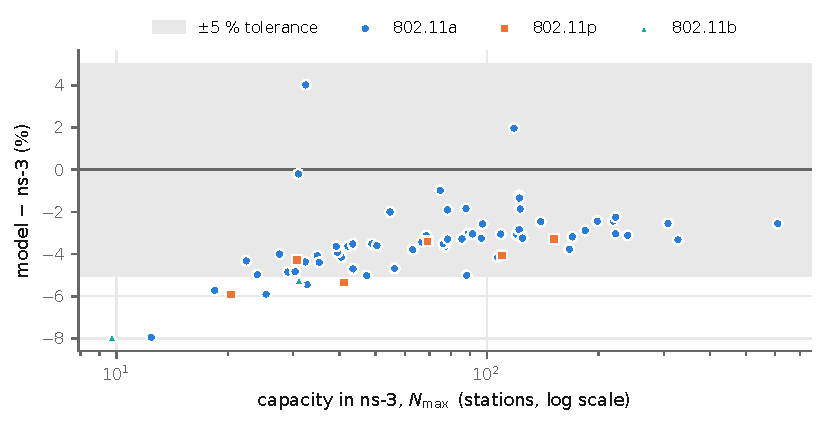
\includegraphics[width=\textwidth]{fig_scorecard}
\caption{The root of \eqref{eq:G5} against \scRows{} capacities stored from ns-3. Below zero, the
model under-predicts the capacity (the safe side).}
\label{fig:scorecard}
\end{figure}

\subsection{The safe side, by traffic source (UJ)}\label{sec:uj}

UJ tested on two new 802.11a cells whether the root of \eqref{eq:G5} stays on the safe side when the
stations' timers jitter or drift, and what frozen phases do (\cref{fig:uj}). It was registered with
two claims for the five non-frozen cells: S, the root at or below ns-3; A, the root and the law
within $\pm5\,\%$. \textbf{S held at all \ujSHeld{}}, the root's error \ujRootMax{} to \ujRootMin\,\%; A held at \ujAHeld, the two misses conservative. With frozen phases (strictly periodic senders,
identical clocks) ns-3's capacity fell by \ujFzDrop\,\% in both cells, to the root
(\ujFzRootMin{} and \ujFzRootMax\,\%) but not past it; the law, which lies slightly above the root,
was optimistic there (\ujFzLawMin{} to \ujFzLawMax\,\%). The registration's outcomes table sent that
case to Mohamed, who decided: \textbf{frozen phases are outside the safe-side claim}. The claim
the report makes is therefore: \emph{the root of \eqref{eq:G5} is on the safe side for timers with
jitter or clock drift} (all new cells, and all stored ones).

\begin{figure}[htbp]
\centering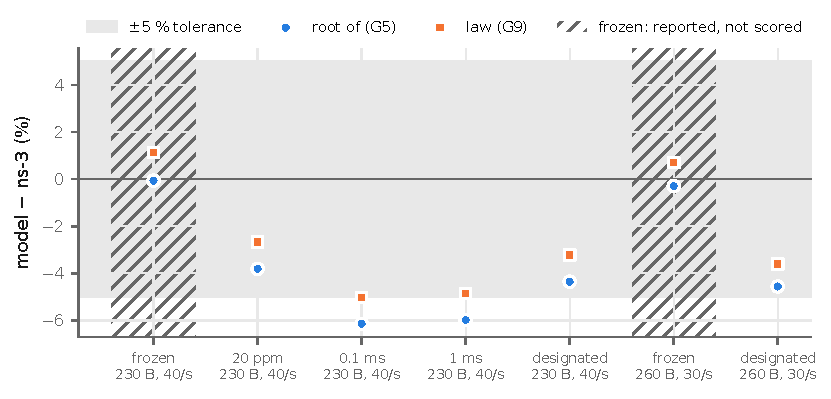
\includegraphics[width=\textwidth]{fig_uj}
\caption{UJ: the error of the root of \eqref{eq:G5} and of the law \eqref{eq:G9} against ns-3, by
traffic source, on two new 802.11a cells. Hatched: frozen phases, reported.}
\label{fig:uj}
\end{figure}

\iffull
\begin{table}[htbp]
\centering\footnotesize
\input{tables/uj}
\caption{UJ in full (S: the root at or below ns-3; A: root and law within $\pm5\,\%$; seed $\sigma$:
the spread of each seed's own crossing).}
\end{table}
\fi

\subsection{The 802.11b arm, and why the sending pattern matters}

At the hardware's own PHY (802.11b, 1\,Mb/s), test UD found the Poisson model low at \udBelow{} of
its \udDOneAll{} small-swarm crossings. At 15--37 stations the root of \eqref{eq:G5} failed the
$\pm5\,\%$ band at \udDRootFailed{} of \udDCells{} cells, all on the safe side (\udDRootMax{} to
\udDRootMin\,\%); at 8--14 stations, with a band widened to $-9\ldots+5\,\%$ at registration, it held
at \udBHeld{} of \udBScored. Term by term, the loss itself was pessimistic by \udThreePMin{} to
\udThreePMax\,\% (D3); a capacity error is far smaller than a loss error because the loss rises
steeply with the load. The cause was the Poisson assumption: ns-3's telemetry source is periodic.
This failure is what \eqref{eq:G25} was written for.

\textbf{UD2 tested \eqref{eq:G25} where UD failed,} on new 802.11b cells at windows 8, 16 and 32 and
loss targets 2, 5 and 10\,\% (\cref{fig:ud2}). It held at all \udQHeld{} of \udQCrossings{}
crossings, with errors from \udQMin{} to \udQMax\,\%, including the \udQPast{} crossings past
occupancy 0.78. The Poisson root beside it erred by \udQPoiMin{} to \udQPoiMax\,\%, outside
$\pm5\,\%$ at \udQPoiOut: UD's failure, repeated on new cells and corrected by \eqref{eq:G25}. UD
itself stays failed as registered.

\begin{figure}[htbp]
\centering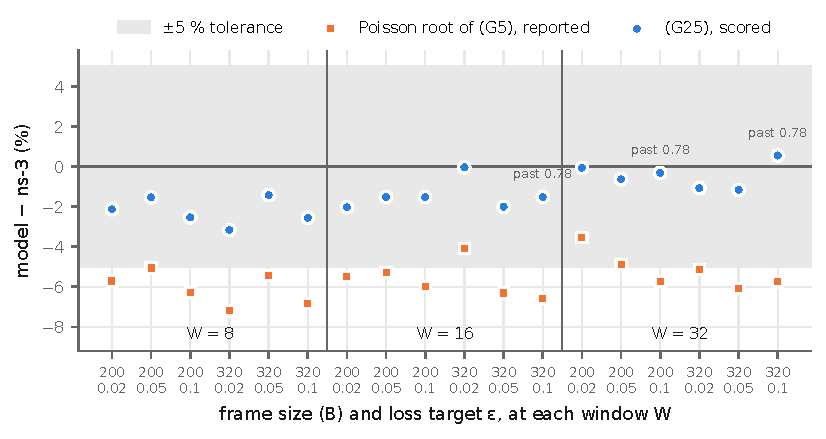
\includegraphics[width=\textwidth]{fig_ud2}
\caption{UD2: \eqref{eq:G25} (scored) and the Poisson root of \eqref{eq:G5} (reported) against
ns-3, 802.11b at 1\,Mb/s, two new frame sizes, three windows and three loss targets.}
\label{fig:ud2}
\end{figure}

\iffull
\begin{table}[htbp]
\centering\footnotesize
\input{tables/ud2}
\caption{UD2 in full, scored at $\pm5\,\%$.}
\end{table}
\fi

\subsection{The sending pattern}

With Poisson sources the model is \ugPoiMin{} to \ugPoiMax\,\% low on the new cells of UG25.
\eqref{eq:G25} was registered on those \ugCells{} cells and held at all \ugHeld{} (\ugMin{} to
\ugMax\,\%). Past occupancy 0.78 (\uhCells{} further cells at occupancy \uhOccMin--\uhOccMax) it is
optimistic by \uhMin{} to \uhMax\,\%, which is now a stated limit (\cref{fig:g25}).

\begin{figure}[htbp]
\centering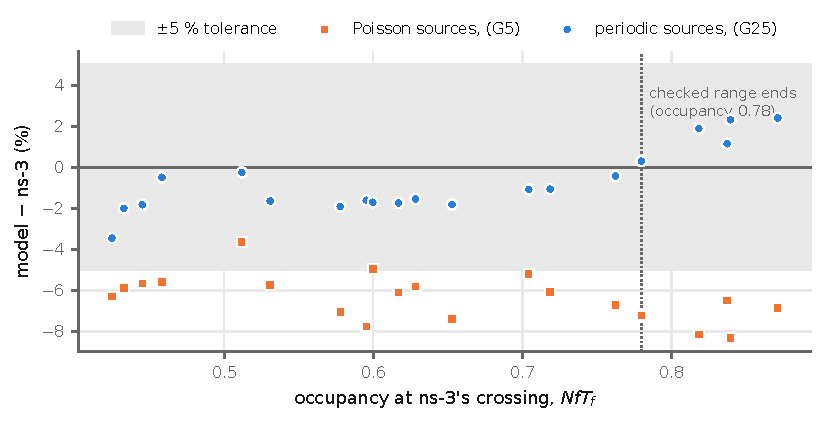
\includegraphics[width=\textwidth]{fig_g25}
\caption{The model's error against ns-3, with Poisson sources, \eqref{eq:G5}, and with periodic
sources, \eqref{eq:G25}, against the occupancy at which ns-3 reaches the loss target.}
\label{fig:g25}
\end{figure}

\subsection{Few stations}

For three to five stations the finite-station form \eqref{eq:FS} held at all \fsHeld{} of \fsCells{}
registered cells, with a tolerance of $\pm15\,\%$ on the loss (\cref{fig:fewstations}). The Poisson
loss \eqref{eq:G5} overstates the loss there by \fsGFiveMin--\fsGFiveMax\,\%.

\begin{figure}[htbp]
\centering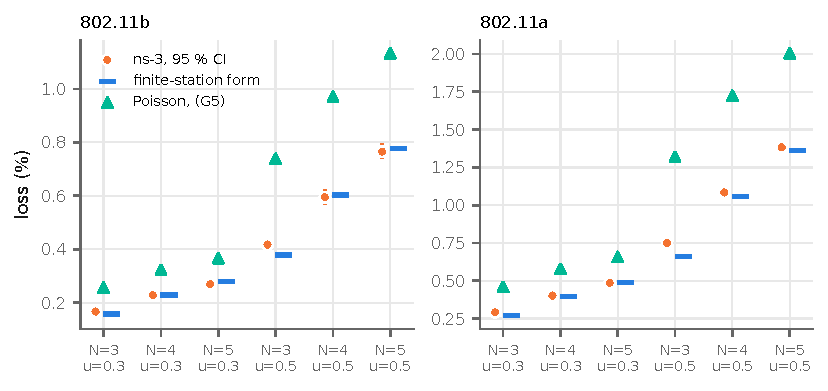
\includegraphics[width=\textwidth]{fig_fewstations}
\caption{UFS: the loss at three to five stations and occupancy 0.3 and 0.5, in ns-3 (30 seeds, 95\,\%
interval), by the finite-station form \eqref{eq:FS} and by the Poisson loss \eqref{eq:G5}.}
\label{fig:fewstations}
\end{figure}

\subsection{Batching}

The gain of batching \eqref{eq:G12} matched ns-3 within \gainMaxAbs\,\% at 802.11a up to 64 records
per frame, and within \gainBMaxAbs\,\% at 802.11b up to 32 (\cref{fig:batching}; reported beside
registered capacity tests UC2 and UD, whose capacities held \ucTwoHeld{} of \ucTwoClaims{} and
\udTwoHeld{} of \udTwoCells).

\begin{figure}[htbp]
\centering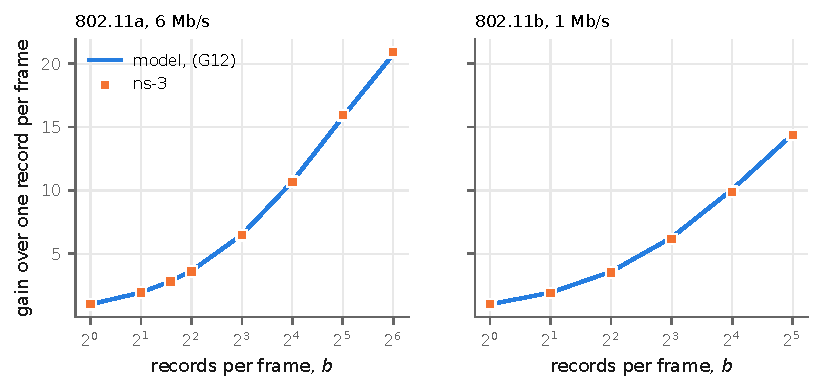
\includegraphics[width=\textwidth]{fig_batching}
\caption{The gain of batching: capacity at $b$ records per frame over capacity at one, less one
station each, \eqref{eq:G12} against ns-3.}
\label{fig:batching}
\end{figure}

\subsection{Capture}

ns-3's capture rule, read from its source and predicted per collision, held at \capHeld{} of
\capTrials{} offsets and power differences (UCAP2). A first capacity test with capture (UF) held
\ufAvgHeld{} of \ufConfigs{} average-delivery claims and only \ufWorstHeld{} of \ufConfigs{}
every-sender claims. Its three causes were found: the half-duplex factor \eqref{eq:G22a} was missing,
the every-sender claim had been scored on a sample minimum rather than on \eqref{eq:G24} or
\eqref{eq:G24a}, and one configuration had a station at the edge of carrier sense. The corrected
test UF2, on new placements and seeds, held all \ufTwoHeld{} of its \ufTwoClaims{} claims, every one
on the safe side: \eqref{eq:G23} within \ufTwoAMin{} to \ufTwoAMax\,\%, the pooled \eqref{eq:G24}
within \ufTwoPoolMin{} to \ufTwoPoolMax\,\%, the window statistic \eqref{eq:G24a} within
\ufTwoWinMin{} to \ufTwoWinMax\,\% (\cref{fig:uf2}).

\begin{figure}[htbp]
\centering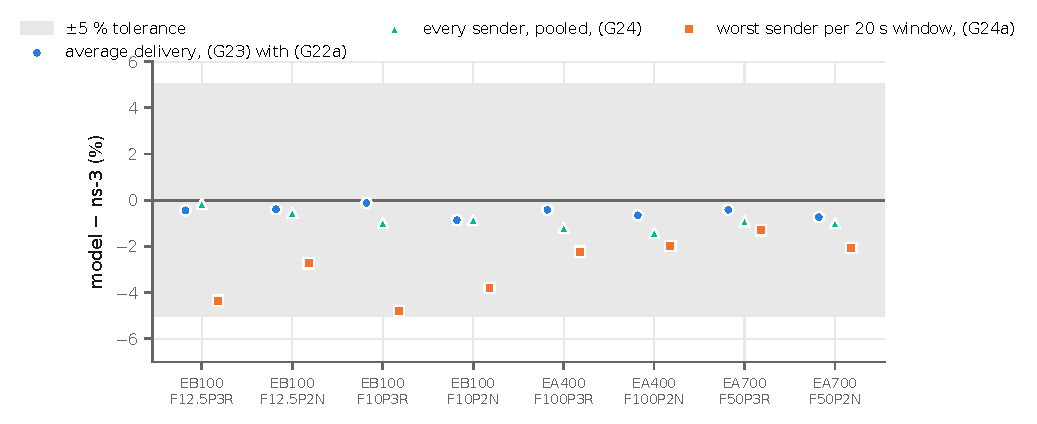
\includegraphics[width=\textwidth]{fig_uf2}
\caption{UF2: the capture laws against ns-3, per configuration (EB: 802.11b, EA: 802.11a; F: frames
per second; P3R: path-loss exponent 3 with Rayleigh fading; P2N: exponent 2, no fading).}
\label{fig:uf2}
\end{figure}

\subsection{Design rules and LoRa}

A key record once in $r=2$ or 4 frames held \ucThreeHeld{} of \ucThreeCells{} (UC3). Fragments spread
over the period held \ucFourSHeld{} of \ucFourSCells{} (UC4S); fragments sent back to back failed
(UC4), and a correction for them removed \burstFixMin--\burstFixMax\,\% of the excess but failed its
own test (UC4B), so the design forbids back-to-back fragments. The best batch under bit errors
\eqref{eq:G19} was predicted as \ucFivePred{} and ns-3's best was \ucFiveBest{} (UC5D1). The LoRa
duty-cycle law held at \lrHeld{} of \lrCells{} cells (UC7).

\subsection{What failed in simulation}

\begin{itemize}
\item \textbf{The split of \eqref{eq:G5} into its three causes} (UC1, D3): the totals hold, the
breakdown does not; ns-3 counts a near-simultaneous start as a detection-window loss.
\item \textbf{Poisson starts at 802.11b} (UD): the capacity \udDRootMax{} to \udDRootMin\,\% low at
15--37 stations; \eqref{eq:G25} then held at all \udQCrossings{} new crossings of UD2.
\item \textbf{The first capture test} (UF): failed for three identified reasons; the corrected test
held on new cells.
\item \textbf{Fragments sent back to back} (UC4, UC4B): outside the model; ruled out by design.
\item \textbf{\eqref{eq:G25} past occupancy 0.78 at 802.11b}: optimistic by \uhMin{} to \uhMax\,\%;
a stated limit.
\item \textbf{Frozen phases} (UJ and the stored cells): ns-3's capacity falls by about
\ujFzDrop\,\%, to the root or past it, and the law is optimistic there (stored: \scLawOptErr\,\%);
excluded from the safe-side claim.
\end{itemize}

% ==================================================================================================
\section{Validation on hardware}\label{sec:hw}
% ==================================================================================================

\textbf{What the hardware tests checked.} W1e, W1j and W1k were registered before the closed form
existed. Their predictions came from the project's event simulation of the DCF access rule
(registered at W1c), which had matched ns-3's capacities at 802.11b within \wOneBErr\,\% (W1b). They test
the access-rule model the closed form is built on, not the closed form's own numbers. W1r's
registration also recorded the closed form's values beside ns-3's; they are compared in
\cref{sec:side}. The first test of the closed form itself on the radios is V1a, below.

\subsection{The closed form on the radios (V1a)}\label{sec:v1a}

On three radios the part of the closed form that applies is the few-station form \eqref{eq:FS}
(three to five stations, occupancy up to 0.5). V1a scored it \emph{as stated}: the standard's window
$\Wnd=32$, rule set A, nothing measured on the radios. The three radios sent at occupancy 0.3, 0.4
and 0.5 in five interleaved rounds, with a control window after each; the session ran remotely and
every validity condition held (background \vaBg\,\%, each radio's link loss alone at most
\vaLinkMax\,\%). The registered tolerance was $\pm15\,\%$ on the loss.

\textbf{The closed form as stated failed at all \vaPoints{} points, on the optimistic side}
(\cref{fig:v1a,tab:v1a}). The radios lost \vaFacMin--\vaFacMax{} times what \eqref{eq:FS} predicts,
and the form lies below the 95\,\% interval of the measurement at every point. ns-3 and the event
simulation, both with the standard rule, sit near the form: the radios lose \vaSimMin--\vaSimMax{}
times what they predict. What misses is therefore the access rule the model assumes, not the
closed form's approximation of that rule. C1 measured the likely cause: the Pi~4s send about half
their frames at DIFS with no backoff, and the Pi~3 waits a fixed \cExtraC\,\us{} longer. A
hardware-matched form, with the radios' measured rule as its input, is the next registered test
(V1b, \cref{sec:next}). The failure was expected and disclosed in the registration; the stored trio
point of W1e and W1r had already pointed to it.

\begin{figure}[htbp]
\centering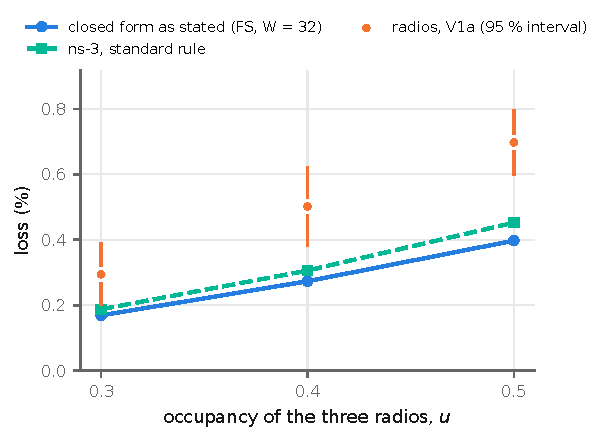
\includegraphics[width=0.66\textwidth]{fig_v1a}
\caption{V1a: the loss of the three radios against the closed form as stated, \eqref{eq:FS} at
$\Wnd=32$, and ns-3 with the standard rule.}
\label{fig:v1a}
\end{figure}

\begin{table}[htbp]
\centering\small
\input{tables/v1a}
\caption{V1a, scored at $\pm15\,\%$. The last three columns were reported, not scored;
\eqref{eq:G5} lies outside its stated range at three stations. Its closeness to the radios
(\vaGfiveMin{} to \vaGfiveMax\,\%) is not evidence for it: periodic sources make it pessimistic for
three stations, while the radios' rule adds collisions, so two departures act in opposite
directions; the matched form will separate them.}
\label{tab:v1a}
\end{table}

\subsection{Contention}

\Cref{fig:hw} shows the loss of two and three radios at occupancy 0.50, 0.70 and 0.85. In W1e (frame
burst on) \weHeld{} of \wePoints{} points lay inside the bands registered from the event
simulation; the miss was pi-A with pi-B at the lowest load, \weMissRatio{} times the prediction against a band
top of \weMissTop. In W1r (frame burst off) the hardware lies between two ns-3 settings of slot and
DIFS: inside the 95\,\% interval at \wrInTwenty{} of \wrPoints{} points for slot 20\,\us/DIFS
50\,\us, and \wrInNine{} for slot 9\,\us/DIFS 28\,\us. The pairs with the Pi 3 lose more than ns-3
predicts; ns-3 had been given windows inferred from each radio's sending rate, $\Wnd=\wrWinPi$ for
the Pi 4s and \wrWinPiThree{} for the Pi 3, and C1 later showed both to be wrong in kind
(\cref{sec:window}).

\begin{figure}[htbp]
\centering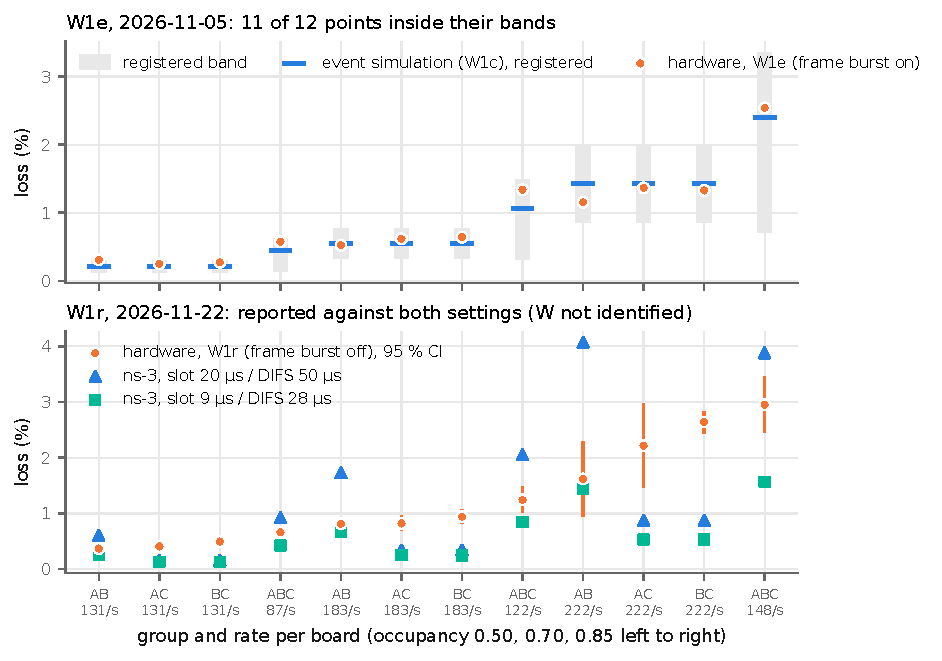
\includegraphics[width=\textwidth]{fig_hw_contention}
\caption{Hardware contention. Top: W1e against its registered prediction (the event simulation of
W1c). Bottom: W1r against ns-3 with two settings of slot and DIFS (the contention window was not
known; \cref{sec:window}).}
\label{fig:hw}
\end{figure}

\subsection{The capacity ratio}

On four radios (pi-A, pi-B, the Pi 3 and the TP-Link), the capacity of the design (one signature per
frame of four records) divided by that of per-record signing was \ratioJ{} in W1j and \ratioK{} in
W1k, against the registered \ratioModel{} (band \ratioLo--\ratioHi; \cref{fig:ratio}). The capacities
themselves were \crossAuthJ{} and \crossPerJ{} capacity-equivalent stations in W1j, against
\crossAuthModel{} and \crossPerModel{} (\crossAuthErr{} and \crossPerErr\,\%), attributed in W1j
to capture at the receivers, while the ratio moved by \ratioErr\,\%.

\begin{figure}[htbp]
\centering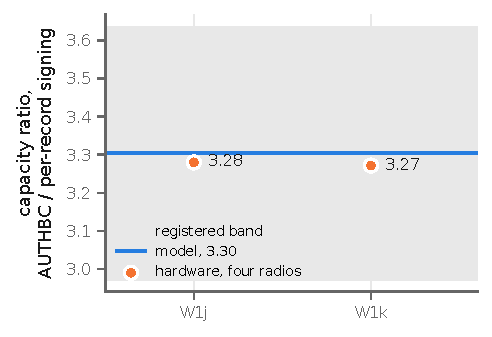
\includegraphics[width=0.5\textwidth]{fig_ratio}
\caption{The capacity ratio on four radios against the registered value.}
\label{fig:ratio}
\end{figure}

\subsection{Loss on air}

W3a traced every frame on air at 802.11b and replayed the traces through the project's real
decoder. All \wtHeld{} of \wtClaims{} registered claims held: real loss hurts the frames that depend
on a key record no more than independent loss would; the design loses only its own frames; and the
loss grows with frame length less steeply than a bit-error model predicts.

\subsection{Capture}

In W1q (the Pi 3 receiving, pi-A's power stepped) \wqHeld{} of \wqScored{} registered predictions
held. The one that failed is the finding: at a measured difference of only \wqThreeDelta\,dB the Pi
3 kept the stronger frame in \wqThreeQ{} of collisions, where ns-3's rule keeps none below 4\,dB.
Capture on this radio is gradual, not a step. Three of W1q's five power steps were void because the
received signal fell by less than the set power (\cref{sec:window}). W1s then tested the gradual
curve on new power steps: \wsCurveHeld{} of \wsCurveScored{} held, so the curve is not used; the
boards' radio geometry had changed between the sessions (\cref{fig:capture}).

\begin{figure}[htbp]
\centering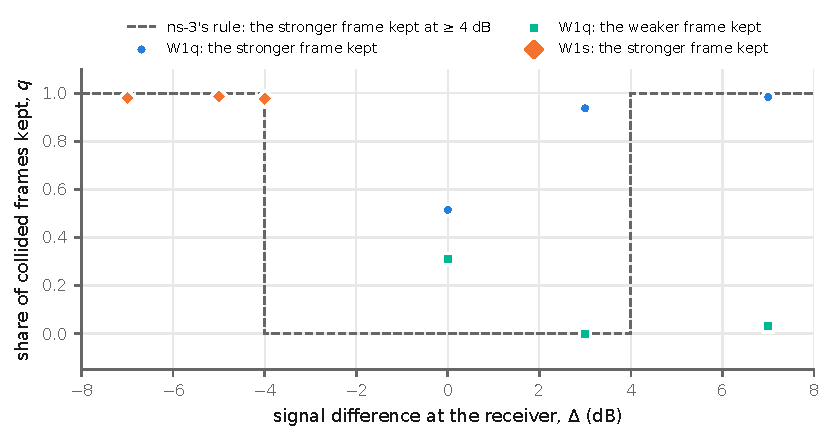
\includegraphics[width=\textwidth]{fig_capture_hw}
\caption{The share of collided frames the receiver kept, against the signal difference. Dashed:
ns-3's 4\,dB rule. W1q's points are from its valid steps; W1s's from its new steps.}
\label{fig:capture}
\end{figure}

\subsection{The contention window, and the radios' own timing}\label{sec:window}

The model needs each radio's contention window $\Wnd$, slot and DIFS; radios do not report them.
\textbf{W1p} tested two settings derived from each radio's sending rate: a saturated pair lost
\wpLoss{} at \wpFps{} frames/s, against ns-3's \wpTwentyLoss{} and \wpNineLoss: neither fits.
\textbf{W1s} re-derived both settings once and tested them at a new frame length: the pair lost
\wsPairLoss{} at \wsPairFps{} frames/s, against \wsTwentyLoss{} and \wsNineLoss: neither fits again,
so the window is recorded as not identifiable without a frame sniffer.

A sniffer was therefore added (the TP-Link in monitor mode, with a one-line driver change that
exports the chip's per-frame hardware timestamp). Its gate S0 \textbf{failed}: it recorded \sgA,
\sgB{} and \sgC{} of the three radios' frames, against the 0.99 required, though the radios
themselves received almost all of them; the misses follow neither the board nor its place, and a
probe at another placement (P1) did not reach 0.99 either; its planned placements 3\,m and 5\,m
away have not run. The same gate showed that the received signal
falls by \sgFalls\,dB when pi-A's set power falls by 3, 6 and 9\,dB; the Pi 3 registered a similar
compression, so the transmitter is the more likely cause, but this is not established. The sniffer
is used for timing only, under a stated rule, until a better adapter arrives.

\textbf{C1 (calibration, not validation)} measured each radio alone with the sniffer's microsecond
timestamps (\cref{fig:c1}). For both Pi 4s the gap after a frame has a floor of \cFloorA\,\us{} (the
standard's DIFS) and a 20\,\us{} lattice (the standard's slot); \cShareMinA--\cShareMaxB{} of their
frames are sent at DIFS with no backoff, and the rest spread over \cWminA{} slots. Under the
standard's rule a saturated sender draws its backoff from $0\ldots\Wnd-1$ after every frame, so only
about $1/\Wnd$ of frames (3\,\% at $\Wnd=32$) would go out at DIFS. Departures of commercial 802.11b cards from the standard's backoff have been
measured before \cite{bianchi2007cards}. The share did not change with a
back-to-back sender (\cShareKA), so it is the radio's own behaviour, not the sending pattern. The
Pi 3's floor is \cFloorC\,\us{} (\cExtraC\,\us{} more than DIFS) and \cShareMinC--\cShareMaxC{} of its
frames skip the backoff, close to the standard's $1/\Wnd$, with \cWminC--\cWmaxC{} slots. Across
frame sizes the airtime grows by \cSlope\,\us{} per byte (1\,Mb/s), with an intercept of
\cInterA\,\us{} (the long preamble, 192\,\us, plus DIFS). These are inputs for a hardware-matched
model; nothing has yet been validated with them.

\begin{figure}[htbp]
\centering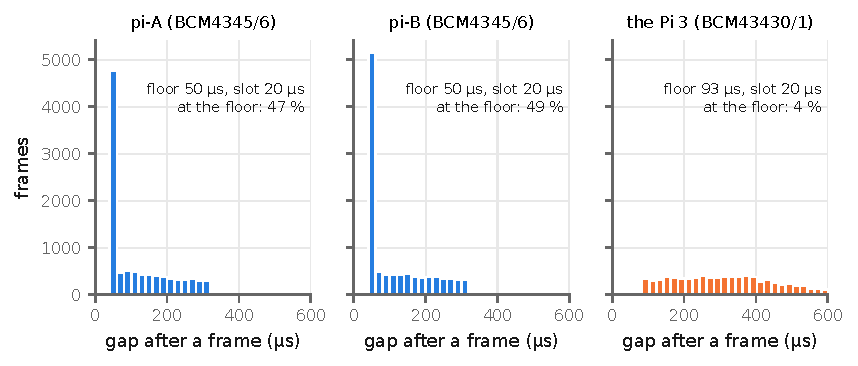
\includegraphics[width=\textwidth]{fig_c1_gaps}
\caption{C1: the gap after each frame, for each radio sending alone (145\,B frames). One bin per
backoff slot.}
\label{fig:c1}
\end{figure}

\iffull
\begin{figure}[htbp]
\centering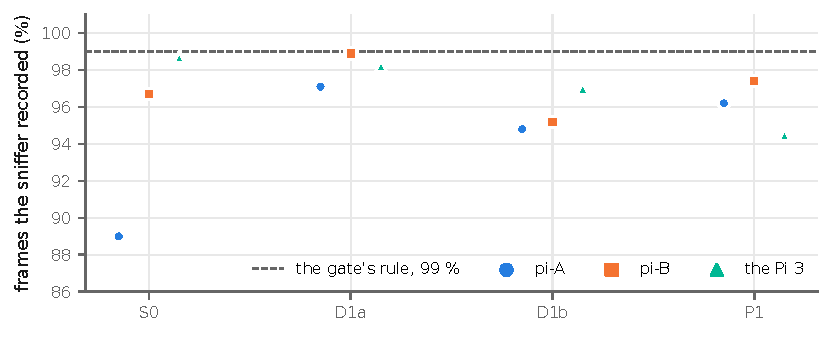
\includegraphics[width=\textwidth]{fig_sniffer}
\caption{The share of each radio's frames the sniffer recorded, session by session (S0: the gate;
D1a, D1b: diagnostics, pi-A and pi-B swapped in D1b; P1: the probe). The misses follow neither the
board nor its place.}
\label{fig:sniffer}
\end{figure}
\fi

\subsection{What failed on hardware}

\begin{itemize}
\item \textbf{The closed form as stated} (V1a): \eqref{eq:FS} at $\Wnd=32$ lies \vaErrB{} to
\vaErrA\,\% from the radios' loss at occupancy 0.3--0.5; the standard access rule is what differs.
\item \textbf{The window, from sending rates} (W1p, W1s): neither setting of slot and DIFS fits; the
window was not identifiable that way. C1 shows why: the Pi 4s skip the backoff for about half their
frames, which no single window describes.
\item \textbf{ns-3's 4\,dB capture step} (W1q): the radio captures at 1.5\,dB; the gradual curve
then failed its own check on new steps (W1s) after the geometry changed.
\item \textbf{The sniffer's gate} (S0, P1): the adapter misses \snifMissMin--\snifMissMax\,\% of frames, drifting between
sessions.
\item \textbf{Power steps}: the received signal falls by less than the set power, most likely at the
transmitter.
\end{itemize}

% ==================================================================================================
\section{Model, simulation and hardware side by side}\label{sec:side}
% ==================================================================================================

\Cref{tab:threeway} puts every source of a prediction beside the two hardware sessions, for the same
radios and rates: the closed forms (as recorded in W1r's registration, at the standard's
$\Wnd=32$), W1c's event simulation (W1e's registered prediction), ns-3 with two settings of slot and
DIFS, and the hardware with frame burst on (W1e) and off (W1r).

\begin{table}[htbp]
\centering\footnotesize
\input{tables/threeway}
\caption{Loss (\%) of two and three radios, 802.11b at 1\,Mb/s, $f$ frames per second per radio.
For the pairs, \eqref{eq:G5} and \eqref{eq:G25} lie outside their stated range (two stations;
\eqref{eq:G25} needs 8 or more others); the finite-station form is shown only where it was accepted
(three stations, occupancy 0.5). The ns-3 values for the pairs with the Pi 3 use its inferred window
of \wrWinPiThree{} slots.}
\label{tab:threeway}
\end{table}

\textbf{What the comparison shows.}
\begin{itemize}
\item \textbf{The trio at occupancy 0.5}, the one point inside every model's range: \eqref{eq:FS},
the event simulation, ns-3 at slot 9\,\us{} and both hardware sessions lie between \twTrioLo{} and
\twTrioHi\,\%; \eqref{eq:G5} and ns-3 at slot 20\,\us{} lie above them.
\item \textbf{The pairs:} no closed form is claimed for two stations. ns-3's values for the pairs
with the Pi 3 are \twPiThreeLo--\twPiThreeHi{} times below the hardware, because ns-3 was given a window of
\wrWinPiThree{} slots for the Pi 3; C1 measured \cWminC--\cWmaxC{} plus a fixed \cExtraC\,\us.
\item \textbf{The same radios, two sessions} (W1e and W1r) differ by up to a factor of \twSessMax{} for the
pairs with the Pi 3: frame burst, placement and day all changed between them. A hardware number is a
property of a session, not only of the radios.
\end{itemize}

\begin{table}[htbp]
\centering\small
\begin{tabularx}{\textwidth}{>{\raggedright\arraybackslash}p{3.9cm}>{\raggedright\arraybackslash}p{2.4cm}>{\raggedright\arraybackslash}p{2.4cm}L}
\toprule
Quantity & Model & ns-3 & Hardware \\
\midrule
loss of three radios at $\occ=0.5$ (V1a) & \vaFinC\,\% \eqref{eq:FS} & \vaNsC\,\% (standard rule) & \vaLossC\,\% \\
capacity ratio, design over per-record signing (4 radios) & \ratioModel{} (event simulation) & -- & \ratioJ, \ratioK{} (W1j, W1k) \\
gain of batching, 802.11a, $b$ up to 64 & \eqref{eq:G12} & within \gainMaxAbs\,\% & not tested (V2) \\
capture at a signal difference of \wqThreeDelta\,dB & \eqref{eq:G22} with the input $q$ & $q=0$ (4\,dB rule) & $q=\wqThreeQ$ (W1q) \\
slot, DIFS & 20\,\us, 50\,\us{} (standard) & the same & 20\,\us, \cFloorA\,\us{} (Pi 4s); 20\,\us, \cFloorC\,\us{} floor (Pi 3) \\
frames sent at DIFS with no backoff, saturated & about $1/\Wnd$ (the standard's backoff after every frame) & not measured & \cShareMinA--\cShareMaxB{} (Pi 4s); \cShareMinC--\cShareMaxC{} (Pi 3) \\
airtime per byte at 1\,Mb/s & 8\,\us & 8\,\us & \cSlope\,\us{} (C1) \\
\bottomrule
\end{tabularx}
\caption{One quantity at a time: what the model assumes or predicts, what ns-3 does, what the radios
do.}
\label{tab:side}
\end{table}

% ==================================================================================================
\section{What remains to be tested}\label{sec:next}
% ==================================================================================================

\Cref{tab:coverage} maps each part of the model against where it has been tested.
\Cref{tab:next} lists the open tests, in the order they can run.

\begin{table}[htbp]
\centering\small
\begin{tabularx}{\textwidth}{>{\raggedright\arraybackslash}p{4.2cm}LL}
\toprule
Part of the model & ns-3 & Hardware \\
\midrule
accounting and batching, \eqref{eq:G1}--\eqref{eq:G3}, \eqref{eq:G10}--\eqref{eq:G13} & held (UC2, UD) & ratio held (W1j, W1k, event simulation); gain on air not tested (V2) \\
loss \eqref{eq:G4}--\eqref{eq:G5} & total held; split into causes failed (UC1) & as stated, \textbf{failed} (V1a, through \eqref{eq:FS}); the radios' access rule differs (C1) \\
two-constant law \eqref{eq:G6}--\eqref{eq:G9} & held where valid, \scLawIn{} of \scLawRows & not tested \\
design rules \eqref{eq:G16}--\eqref{eq:G21} & held (UC3, UC4S, UC5D1, UC7); back-to-back fragments failed & not tested \\
capture \eqref{eq:G22}--\eqref{eq:G24a} & held after correction (UCAP2, UF2) & the input $q$ measured, partly (W1q); in contention not tested (V3, V4) \\
sending pattern \eqref{eq:G25}, \eqref{eq:FS} & held to occupancy 0.78, and at 802.11b at every window and target (UD2); 3--5 stations held & \eqref{eq:FS} as stated \textbf{failed} (V1a); with the measured rule: V1b \\
hidden stations; two stations & not tested; no closed form & not tested \\
\bottomrule
\end{tabularx}
\caption{The coverage map: where each part of the model has been tested, and how it came out.}
\label{tab:coverage}
\end{table}

\begin{table}[htbp]
\centering\small
\begin{tabularx}{\textwidth}{>{\raggedright\arraybackslash}p{3.6cm}>{\raggedright\arraybackslash}p{1.9cm}L>{\raggedright\arraybackslash}p{2.9cm}}
\toprule
Test & Where & What it would show & Waits on \\
\midrule
S0b: the AR9271 sniffer's gate, beside the TP-Link & hardware & whether a second sniffer records $\ge99\,\%$ of frames; whether the power steps compress at the sender & the adapter (by 30 November 2026) \\
C1 in W1q's layout (L1); P1 at 3\,m and 5\,m & hardware & the timing of C1 where the capture sessions ran; whether distance lets the TP-Link reach 0.99 & Mohamed at the boards \\
C2: saturated pairs with the sniffer & hardware & the access rule two radios use under contention: who skips the backoff, and when & S0b \\
C3: the capture curve, both signs of the signal difference & hardware & $q$ against the signal difference for the real receiver & S0b \\
The parameter file & -- & the measured slot, DIFS, access rule, airtime and link losses, as one input set & C1--C3; Mohamed's review \\
The hardware-matched form: \eqref{eq:FS} with each radio's measured backoff and fixed delay, checked against the event simulation & model & the closed form with the radios' own rule, derived and checked before any test & Mohamed's acceptance of the derivation \\
V1b: the matched form on a new session of the three radios, as V1a & hardware & whether the closed form predicts the radios once it is given their rule & C2; the parameter file \\
V2: batching on air & hardware & the gain \eqref{eq:G12} on real radios & the parameter file \\
V3, V4: capture in contention; every-sender statistics & hardware & \eqref{eq:G22}--\eqref{eq:G24a} on real radios & C3 \\
Transmitter or receiver: does pi-A's output follow its set power? & hardware & where the power steps compress & an external receiver (HackRF) if S0b cannot separate them \\
Hidden stations & ns-3 & the term $2h\nu\Tf$ & outside the current scope \\
Two stations; fragments sent back to back & model & a closed form (none exists) & a derivation \\
\bottomrule
\end{tabularx}
\caption{The open tests. Calibration (C) sets the inputs; validation (V) tests predictions made from
them; no session does both.}
\label{tab:next}
\end{table}

If no suitable adapter is available by 30 November 2026, C2 and C3 use the receivers' logs, as W1p
and W1q did, with the sniffer for timing only, and the report of those sessions states the
limitation.

% ==================================================================================================
\section{Conclusions}
% ==================================================================================================

\begin{itemize}
\item \textbf{What can be claimed now.} The closed form predicts ns-3's capacity within $\pm5\,\%$ in
\scRootIn{} of \scRows{} stored cases, and its root lies on the safe side for every timer with jitter
or clock drift (UJ); frozen phases are excluded. Its extensions
for the sending pattern and for capture hold in registered ns-3 tests on new cells. On hardware, the
capacity ratio of the design over per-record signing matches the registered value (\ratioJ{}
against \ratioModel), and the access-rule model behind the closed form fell inside the registered
bands at \weHeld{} of \wePoints{} contention points.
\item \textbf{What cannot be claimed yet.} That the closed form predicts the radios' loss: as stated,
with the standard's access rule, it does not (V1a: the radios lose \vaFacMin--\vaFacMax{} times its
prediction, and ns-3 with the same rule misses alike); whether it does with the radios' measured
rule is the next test (V1b). That the model's access rule is the radios': the Pi 4s send about
half their frames with no backoff, which the standard's rule does not include. That ns-3's 4\,dB
capture step describes the real receiver: it captures gradually.
\item \textbf{Next.} The hardware-matched form (derived, then checked against the event simulation);
a sniffer that passes its gate and the calibration sessions C2 and C3; the parameter file for
review; then V1b and the validation sessions V2--V4 against the matched model and ns-3.
\end{itemize}

\iffull
\appendix
% ==================================================================================================
\section{Notation}
% ==================================================================================================
\begin{table}[htbp]
\centering\small
\begin{tabular}{ll}
\toprule
Symbol & Meaning \\
\midrule
$\Lam$ & records per second per station \\
$b$, $\bstar$, $\bM$ & batch (records per frame); the batch used; the largest that fits \\
$\Dmax$, $\Dnet$, $\Sq$ & deadline; deadline net of the delay $\Sq$ \\
$\Phi$, $\Psi$, $\Bud$ & cost per frame, cost per record, budget of a resource \\
$\Tf$ & a frame's airtime \\
$f$, $\nu$ & frames per second per station; start rate of the other stations, $(N-1)f$ \\
$\occ$ & occupancy, $N f\Tf$ \\
$\slot$, $\Difs$, $\Wnd$, $\delta$ & slot, DIFS, contention window, preamble-detection time \\
$\eps$, $\eps'$, $\epsw$ & loss target; with capture, average; with capture, every sender \\
$\rhostar$, $\tauzero$, $\tauhat$, $\kappa$ & the two constants of \eqref{eq:G9}; per-frame channel cost; $1-\eps/2$ \\
$\Kbar$, $a$, $\gamma$, $\eta$ & co-waiting frames; busy, gap and immediate-access loads \\
$\pcoll$, $q$, $\qeff$, $\ell$, $\ellbar$ & collision loss; capture probability; with the half-duplex factor; link loss; its average \\
$\Ninf$, $\beta$, $\Gain$ & capacity limit, half-gain batch, gain of batching \\
$\Rper$ & periodic-source ratio of \eqref{eq:G25} \\
$m$, $M$, $\pi$ & bystanders, co-waiting count and co-waiting probability of \eqref{eq:FS} \\
$z_N$ & expected maximum of $N$ standard normal draws \\
\bottomrule
\end{tabular}
\end{table}

% ==================================================================================================
\section{Failed attempts and corrections, kept visible}
% ==================================================================================================

\begin{itemize}
\item \textbf{UF (capture, first test).} \ufAvgHeld{} of \ufConfigs{} and \ufWorstHeld{} of
\ufConfigs{} held. Three causes, each found from logged state, not assumed: the half-duplex factor
\eqref{eq:G22a} had been omitted from both the law and its check script, so their agreement could not
reveal it; the every-sender claim had been scored on a sample minimum, an extreme that grows with
the number of senders, rather than on \eqref{eq:G24} or \eqref{eq:G24a}; one configuration placed a
station at the edge of carrier sense, outside one collision domain. UF stays failed; UF2 tested the
corrections on new placements and seeds.
\item \textbf{UC4B (a burst correction for back-to-back fragments).} Removed
\burstFixMin--\burstFixMax\,\% of the excess but failed on both scored cells, on the optimistic
side. Not used; the design rule forbids the case.
\item \textbf{UG25H: \eqref{eq:G25} at high occupancy.} An earlier estimate from capture runs put
the error at \fOneFortyMin--\fOneFortyMax\,\%; measured once without capture it is \uhMin{} to \uhMax\,\%. The band of
the earlier estimate held at none of the four cells.
\item \textbf{W1p and W1s (the window from sending rates).} Two re-derivations, two failures; by
Mohamed's rule no third attempt was made, and the window was recorded as not identifiable without a
sniffer.
\item \textbf{W1q's gradual capture curve.} Fitted after W1q's failure, then checked on new steps in
W1s: \wsCurveHeld{} of \wsCurveScored{}; not used.
\item \textbf{S0's timing criterion.} The registration compared the median of the sniffer's
start-to-start intervals with the receivers' mean cycle; with half the gaps at DIFS the median was
bound to fall below the mean. The means agree within \sZeroMeanMin--\sZeroMeanMax\,\%. A corrected gate (S0b) compares
mean with mean on new windows.
\item \textbf{C1's estimators.} Two estimators were revised after the gate's rate checks and before
C1 ran (the lattice had picked a harmonic; $\Wnd-1$ from a percentile read the long tail); both were
tested on synthetic gaps of known slot and window first, and the revision is disclosed in C1's
registration.
\end{itemize}

\FloatBarrier
% ==================================================================================================
\section{Every test, in full}
% ==================================================================================================

Each table is generated from the test's scored file in \texttt{results/raw/}.

\subsection{Simulation}

{\footnotesize\setlength{\tabcolsep}{3pt}
\renewcommand{\longcap}{Every stored ns-3 capacity against the law \eqref{eq:G9} and the root of
\eqref{eq:G5} (errors in \%; negative is the safe side; ``--'': the law is not valid for that
frame).\label{tab:scorecard}}
\input{tables/scorecard}
}

\begin{table}[htbp]
\centering\footnotesize
\input{tables/ud}
\caption{UD, the 802.11b arm: D1, small swarms at three windows and loss targets (Pb1B: 8--14
stations, band $-9\ldots+5\,\%$, not scored below 8 stations; Pb1D: 15--37 stations, band
$\pm5\,\%$); D2, batches of 1--32 records.}
\end{table}

\begin{table}[htbp]
\centering\footnotesize
\input{tables/ug25}
\caption{UG25: \eqref{eq:G25} on new cells, $\pm5\,\%$; last four rows, UG25H: 802.11b past
occupancy 0.78, measured, not scored.}
\end{table}

\begin{table}[htbp]
\centering\footnotesize
\input{tables/uf2}
\caption{UF2: capacities (stations) with capture; (a) the average criterion \eqref{eq:G23} with
\eqref{eq:G22a}; statistic 1, the pooled every-sender loss \eqref{eq:G24}; statistic 2, the window
statistic \eqref{eq:G24a}. Tolerance $\pm5\,\%$.}
\end{table}

\begin{table}[htbp]
\centering\footnotesize
\input{tables/ufs}
\caption{UFS: the finite-station form \eqref{eq:FS} against ns-3's loss, tolerance $\pm15\,\%$; the
last two columns are the errors of \eqref{eq:G5} and \eqref{eq:G25}, reported.}
\end{table}

\begin{table}[htbp]
\centering\footnotesize
\input{tables/uc7}
\caption{UC7: the LoRa duty-cycle law against ns-3's LoRaWAN module (D: duty cycle in \%; C:
channels; L: payload in bytes).}
\end{table}

\FloatBarrier
\subsection{Hardware}

\begin{table}[htbp]
\centering\footnotesize
\input{tables/w1e}
\caption{W1e: contention, frame burst on; measured loss less the background, against the event
simulation registered at W1c.}
\end{table}

\begin{table}[htbp]
\centering\footnotesize
\input{tables/w1r}
\caption{W1r: contention, frame burst off, against ns-3 with the windows inferred from sending
rates (for the trio, equal power to Rayleigh with capture).}
\end{table}

\begin{table}[htbp]
\centering\footnotesize
\input{tables/w1q}
\caption{W1q: the capture steps as recorded (the Pi 3 receives; $q_A$, $q_B$: the share of
collided frames kept from pi-A and pi-B).}
\end{table}

\begin{table}[htbp]
\centering\footnotesize
\input{tables/w1s}
\caption{W1s, part A: the capture curve's new steps, as recorded.}
\end{table}

\begin{table}[htbp]
\centering\footnotesize
\input{tables/s0}
\caption{S0: the sniffer's gate, as recorded.}
\end{table}

\begin{table}[htbp]
\centering\footnotesize\setlength{\tabcolsep}{3.5pt}
\input{tables/c1}
\caption{C1 (calibration): each radio alone, saturated (R: rate checks; Q: redrawn sender at 600
frames/s; K: back-to-back). ``Recorded'': the sniffer's share of the frames sent; ``strict'': pairs
whose neighbours were also recorded. The 50 frames/s windows give link losses, not timing, and are
left out.}
\end{table}

\FloatBarrier
% ==================================================================================================
\section{Where every number comes from}
% ==================================================================================================
Every result in this report is a macro written by \texttt{analysis/report\_numbers.py} from the
project's stored results, or a cell of a table it generates. \Cref{tab:provenance} names each
macro's file and registration; \texttt{provenance.csv} beside this report holds the same list. The
figures are drawn by \texttt{analysis/report\_figures.py} from the same files. To rebuild:
\begin{verbatim}
python analysis/report_numbers.py
python analysis/report_figures.py
cd docs/reports/2026-11-27_model_report && ./build.sh
\end{verbatim}

{\footnotesize\setlength{\tabcolsep}{3pt}
\renewcommand{\longcap}{Every macro, its value, its file and its registration or meaning.\label{tab:provenance}}
\input{tables/provenance}
}
\fi

\bibliographystyle{unsrt}
\bibliography{refs}

\end{document}
"
% build.sh builds both. Every result comes from numbers.tex or tables/ (analysis/report_numbers.py);
% every figure from analysis/report_figures.py; every symbol from notation.tex.
\documentclass[11pt,a4paper]{article}
\usepackage[T1]{fontenc}
\usepackage{lmodern}
\usepackage{textcomp}
\usepackage[margin=2.3cm]{geometry}
\usepackage{amsmath,amssymb}
\usepackage{booktabs,tabularx,array,longtable}
\usepackage{graphicx}
\usepackage[table]{xcolor}
\usepackage{tikz}
\usetikzlibrary{arrows.meta,positioning}
\usepackage{enumitem}
\usepackage[font=small,labelfont=bf]{caption}
\usepackage[hidelinks]{hyperref}
\usepackage{cleveref}
\usepackage{placeins}
\setlength{\parindent}{0pt}
\setlength{\parskip}{0.5em}
\setlist{itemsep=0.15em,topsep=0.3em}
\newif\iffull
\ifdefined\FULL\fulltrue\fi
% Notation of the model report: one macro per symbol, used in every equation and in the
% notation table, so that a symbol cannot drift between sections or between the two versions.
% The symbols are those of docs/revision/unified_closed_form_model.md.
\newcommand{\Nmax}{N_{\max}}                 % capacity: the largest swarm meeting the loss target
\newcommand{\Lam}{\Lambda}                   % records per second per station
\newcommand{\Dmax}{D_{\max}}                 % freshness deadline
\newcommand{\Dnet}{D'}                       % the deadline net of channel and verification delay
\newcommand{\Sq}{S_q}                        % channel and verification delay
\newcommand{\bstar}{b^{\ast}}                % the batch used
\newcommand{\bM}{b_M}                        % the largest batch that fits a frame
\newcommand{\Bud}{\mathrm{B}}                % a resource's budget
\newcommand{\Tf}{T_f}                        % a frame's airtime
\newcommand{\Difs}{\mathrm{DIFS}}            % DCF interframe space
\newcommand{\slot}{\sigma}                   % backoff slot time
\newcommand{\Wnd}{W}                         % contention window: backoff drawn from 0 ... W-1
\newcommand{\eps}{\varepsilon}               % loss target
\newcommand{\rhostar}{\rho^{\ast}}           % occupancy ceiling of the two-constant law
\newcommand{\tauzero}{\tau_0}                % protocol time of the two-constant law
\newcommand{\tauhat}{\hat\tau}               % per-frame channel cost beyond the airtime
\newcommand{\Kbar}{\bar K}                   % mean number of co-waiting frames
\newcommand{\pcoll}{p_c}                     % collision loss: the loss expression (G5)
\newcommand{\occ}{u}                         % occupancy, N f T_f
\newcommand{\qbar}{\bar q}                   % capture probability averaged over senders/receivers
\newcommand{\qeff}{\bar q_{\mathrm{eff}}}    % with the half-duplex factor
\newcommand{\epsw}{\eps_{w}}                 % the every-sender loss target
\newcommand{\Ninf}{N_{\infty}}               % capacity if only the per-record cost existed
\newcommand{\Gain}{\Gamma}                   % the gain of batching
\newcommand{\phat}{\hat p}                   % an observed loss in a window
\newcommand{\Rper}{R}                        % the periodic-source ratio of (G25)
\newcommand{\Rx}{\mathrm{R}}                 % a radio's bit rate
\newcommand{\dB}{\ensuremath{\,\mathrm{dB}}}
\newcommand{\us}{\ensuremath{\,\mu\mathrm{s}}}
% equation sources: every numbered equation is followed by one \src line
\newcommand{\ellbar}{\bar\ell}               % link loss averaged over links
\newcommand{\longcap}{}                      % the caption of the next generated long table
\newcommand{\src}[1]{\par\noindent{\small\textit{Source:} #1}\par\smallskip}

% Generated by analysis/report_numbers.py from results/raw; do not edit by hand.
\newcommand{\scRows}{74}
\newcommand{\scLawRows}{67}
\newcommand{\scLawIn}{62}
\newcommand{\scRootIn}{64}
\newcommand{\scLawMeanAbs}{2.3}
\newcommand{\scRootMeanAbs}{3.6}
\newcommand{\scLawSafe}{60}
\newcommand{\scRootSafe}{72}
\newcommand{\scRootOut}{10}
\newcommand{\scRootOutSafe}{10}
\newcommand{\scLawOut}{5}
\newcommand{\scLawOutSafe}{4}
\newcommand{\scLawOptN}{1}
\newcommand{\scLawOptErr}{+6.4}
\newcommand{\scARows}{66}
\newcommand{\scARootIn}{60}
\newcommand{\scARootMin}{\textminus{}7.9}
\newcommand{\scARootMax}{+4.0}
\newcommand{\scPRows}{6}
\newcommand{\scPRootIn}{4}
\newcommand{\scPRootMin}{\textminus{}5.9}
\newcommand{\scPRootMax}{\textminus{}3.3}
\newcommand{\scBRows}{2}
\newcommand{\scBRootIn}{0}
\newcommand{\scBRootMin}{\textminus{}7.9}
\newcommand{\scBRootMax}{\textminus{}5.2}
\newcommand{\ugCells}{16}
\newcommand{\ugHeld}{16}
\newcommand{\ugMin}{\textminus{}3.4}
\newcommand{\ugMax}{+0.3}
\newcommand{\ugPoiMin}{\textminus{}7.8}
\newcommand{\ugPoiMax}{\textminus{}3.6}
\newcommand{\uhCells}{4}
\newcommand{\uhMin}{+1.16}
\newcommand{\uhMax}{+2.41}
\newcommand{\uhOccMin}{0.82}
\newcommand{\uhOccMax}{0.87}
\newcommand{\capTrials}{552}
\newcommand{\capHeld}{552}
\newcommand{\ufConfigs}{16}
\newcommand{\ufAvgHeld}{12}
\newcommand{\ufWorstHeld}{2}
\newcommand{\ufTwoClaims}{24}
\newcommand{\ufTwoHeld}{24}
\newcommand{\ufTwoAMin}{\textminus{}0.86}
\newcommand{\ufTwoAMax}{\textminus{}0.12}
\newcommand{\ufTwoWinMin}{\textminus{}4.79}
\newcommand{\ufTwoWinMax}{\textminus{}1.30}
\newcommand{\ufTwoPoolMin}{\textminus{}1.41}
\newcommand{\ufTwoPoolMax}{\textminus{}0.15}
\newcommand{\fsCells}{12}
\newcommand{\fsHeld}{12}
\newcommand{\lrCells}{18}
\newcommand{\lrHeld}{12}
\newcommand{\gainMaxAbs}{0.9}
\newcommand{\ucTwoClaims}{6}
\newcommand{\ucTwoHeld}{6}
\newcommand{\udBScored}{5}
\newcommand{\udBHeld}{5}
\newcommand{\udDCells}{9}
\newcommand{\udDRootFailed}{8}
\newcommand{\udDLawFailed}{9}
\newcommand{\udDRootMin}{\textminus{}6.3}
\newcommand{\udDRootMax}{\textminus{}5.0}
\newcommand{\udBelow}{18}
\newcommand{\udDOneAll}{18}
\newcommand{\udTwoCells}{6}
\newcommand{\udTwoHeld}{6}
\newcommand{\gainBMaxAbs}{1.9}
\newcommand{\ucOneHeld}{17}
\newcommand{\ucOneCases}{48}
\newcommand{\ucOnePHeld}{7}
\newcommand{\ucOnePCases}{8}
\newcommand{\ucOnePMin}{+2.5}
\newcommand{\ucOnePMax}{+13.2}
\newcommand{\udThreeHeld}{18}
\newcommand{\udThreeCases}{48}
\newcommand{\udThreePHeld}{0}
\newcommand{\udThreePCases}{8}
\newcommand{\udThreePMin}{+13.9}
\newcommand{\udThreePMax}{+44.3}
\newcommand{\ucThreeHeld}{2}
\newcommand{\ucThreeCells}{2}
\newcommand{\ucFourRootFailed}{2}
\newcommand{\ucFourCells}{2}
\newcommand{\ucFourSHeld}{2}
\newcommand{\ucFourSCells}{2}
\newcommand{\ucFiveBest}{8}
\newcommand{\ucFivePred}{8}
\newcommand{\wtHeld}{3}
\newcommand{\wtClaims}{3}
\newcommand{\weHeld}{11}
\newcommand{\wePoints}{12}
\newcommand{\ratioJ}{3.28}
\newcommand{\ratioModel}{3.30}
\newcommand{\ratioLo}{2.97}
\newcommand{\ratioHi}{3.63}
\newcommand{\crossAuthJ}{30.5}
\newcommand{\crossAuthModel}{29.5}
\newcommand{\crossPerJ}{9.3}
\newcommand{\crossPerModel}{8.9}
\newcommand{\ratioK}{3.27}
\newcommand{\crossAuthK}{30.7}
\newcommand{\crossPerK}{9.4}
\newcommand{\wpLoss}{0.1029}
\newcommand{\wpFps}{262.7}
\newcommand{\wpTwentyLoss}{0.413}
\newcommand{\wpTwentyFps}{331}
\newcommand{\wpNineLoss}{0.169}
\newcommand{\wpNineFps}{288}
\newcommand{\wqHeld}{5}
\newcommand{\wqScored}{6}
\newcommand{\wqThreeDelta}{1.5}
\newcommand{\wqThreeQ}{0.937}
\newcommand{\wrPoints}{12}
\newcommand{\wrInTwenty}{2}
\newcommand{\wrInNine}{1}
\newcommand{\wsCurveHeld}{2}
\newcommand{\wsCurveScored}{3}
\newcommand{\wsPairLoss}{0.1019}
\newcommand{\wsPairFps}{145.6}
\newcommand{\wsTwentyLoss}{0.1227}
\newcommand{\wsTwentyFps}{149.5}
\newcommand{\wsNineLoss}{0.0686}
\newcommand{\wsNineFps}{145.9}
\newcommand{\wsD}{158}
\newcommand{\wsC}{265}
\newcommand{\sgA}{0.890}
\newcommand{\sgB}{0.967}
\newcommand{\sgC}{0.987}
\newcommand{\sgFalls}{2.1, 4.0, 6.5}
\newcommand{\cFloorA}{50}
\newcommand{\cShareMinA}{0.45}
\newcommand{\cShareMaxA}{0.47}
\newcommand{\cShareKA}{0.47}
\newcommand{\cWminA}{13}
\newcommand{\cWmaxA}{13}
\newcommand{\cFloorB}{50}
\newcommand{\cShareMinB}{0.45}
\newcommand{\cShareMaxB}{0.49}
\newcommand{\cShareKB}{0.48}
\newcommand{\cWminB}{13}
\newcommand{\cWmaxB}{13}
\newcommand{\cFloorC}{93}
\newcommand{\cShareMinC}{0.03}
\newcommand{\cShareMaxC}{0.04}
\newcommand{\cShareKC}{0.03}
\newcommand{\cWminC}{22}
\newcommand{\cWmaxC}{25}
\newcommand{\cSlope}{8.00}
\newcommand{\cInterA}{242}
\newcommand{\cInterC}{285}
\newcommand{\fsGFiveMin}{35}
\newcommand{\fsGFiveMax}{77}
\newcommand{\weMissRatio}{1.44}
\newcommand{\weMissTop}{1.40}
\newcommand{\crossAuthErr}{+3.3}
\newcommand{\crossPerErr}{+4.1}
\newcommand{\ratioErr}{\textminus{}0.7}
\newcommand{\twPiThreeLo}{2.4}
\newcommand{\twPiThreeHi}{5.0}
\newcommand{\twSessMax}{2.0}
\newcommand{\twTrioLo}{0.40}
\newcommand{\twTrioHi}{0.66}
\newcommand{\wkRatioLaw}{3.6}
\newcommand{\wkRatioNs}{3.5}
\newcommand{\snifMissMin}{0.7}
\newcommand{\snifMissMax}{11.0}
\newcommand{\kRhoA}{0.595}
\newcommand{\kTauA}{98}
\newcommand{\vaPoints}{3}
\newcommand{\vaHeld}{0}
\newcommand{\vaLossA}{0.294}
\newcommand{\vaLoA}{0.198}
\newcommand{\vaHiA}{0.391}
\newcommand{\vaFinA}{0.169}
\newcommand{\vaNsA}{0.188}
\newcommand{\vaErrA}{\textminus{}42.7}
\newcommand{\vaLossB}{0.501}
\newcommand{\vaLoB}{0.378}
\newcommand{\vaHiB}{0.625}
\newcommand{\vaFinB}{0.273}
\newcommand{\vaNsB}{0.306}
\newcommand{\vaErrB}{\textminus{}45.5}
\newcommand{\vaLossC}{0.697}
\newcommand{\vaLoC}{0.597}
\newcommand{\vaHiC}{0.798}
\newcommand{\vaFinC}{0.397}
\newcommand{\vaNsC}{0.452}
\newcommand{\vaErrC}{\textminus{}43.0}
\newcommand{\vaFacMin}{1.74}
\newcommand{\vaFacMax}{1.84}
\newcommand{\vaSimMin}{1.52}
\newcommand{\vaSimMax}{1.64}
\newcommand{\vaGfiveMin}{\textminus{}11}
\newcommand{\vaGfiveMax}{+6}
\newcommand{\vaBg}{0.11}
\newcommand{\vaLinkMax}{0.18}
\newcommand{\udQCrossings}{18}
\newcommand{\udQHeld}{18}
\newcommand{\udQMin}{\textminus{}3.16}
\newcommand{\udQMax}{+0.56}
\newcommand{\udQPoiMin}{\textminus{}7.2}
\newcommand{\udQPoiMax}{\textminus{}3.6}
\newcommand{\udQPoiOut}{15}
\newcommand{\udQPast}{3}
\newcommand{\udQPastHeld}{3}
\newcommand{\ujScored}{5}
\newcommand{\ujSHeld}{5}
\newcommand{\ujAHeld}{3}
\newcommand{\ujRootMin}{\textminus{}6.1}
\newcommand{\ujRootMax}{\textminus{}3.8}
\newcommand{\ujFzRootMin}{\textminus{}0.30}
\newcommand{\ujFzRootMax}{\textminus{}0.07}
\newcommand{\ujFzLawMin}{+0.70}
\newcommand{\ujFzLawMax}{+1.13}
\newcommand{\ujFzDrop}{4.3}
\newcommand{\cExtraC}{43}
\newcommand{\evRootWorst}{6.5}
\newcommand{\evRootSmall}{9}
\newcommand{\evSafe}{44}
\newcommand{\evCases}{45}
\newcommand{\evSatErr}{3}
\newcommand{\evGainErr}{2}
\newcommand{\evCapErr}{3.1}
\newcommand{\evRuleVar}{5}
\newcommand{\evRatioVar}{2}
\newcommand{\evVarS}{1}
\newcommand{\fragBurstMin}{1.7}
\newcommand{\fragBurstMax}{2.3}
\newcommand{\fragCapMin}{35}
\newcommand{\fragCapMax}{62}
\newcommand{\fragSpread}{3}
\newcommand{\burstFixMin}{63}
\newcommand{\burstFixMax}{75}
\newcommand{\keyRatio}{0.88}
\newcommand{\keyShare}{12}
\newcommand{\capGain}{15}
\newcommand{\smallMin}{5}
\newcommand{\smallMax}{11}
\newcommand{\fOneFortyMin}{3.6}
\newcommand{\fOneFortyMax}{5.5}
\newcommand{\evTwoFrame}{95}
\newcommand{\rQueueErr}{0.07}
\newcommand{\wrWinPi}{4}
\newcommand{\wrWinPiThree}{51}
\newcommand{\sZeroMeanMin}{0.03}
\newcommand{\sZeroMeanMax}{0.25}
\newcommand{\wOneBErr}{1}

\graphicspath{{figures/}}
\newcolumntype{L}{>{\raggedright\arraybackslash}X}
\newcommand{\plain}[1]{\par\smallskip\noindent\fcolorbox{black!20}{black!3}{\parbox{\dimexpr\linewidth-2\fboxsep-2\fboxrule}{\small\textbf{In plain words.} #1}}\par\smallskip}
\renewcommand{\topfraction}{0.9}
\renewcommand{\bottomfraction}{0.8}
\renewcommand{\textfraction}{0.07}
\renewcommand{\floatpagefraction}{0.8}
\crefname{equation}{}{}

\title{\textbf{A Closed-Form Capacity Model for Authenticated, Batched UAV Telemetry over 802.11}\\[0.4em]
\large The model, its sources, and its validation in simulation and on hardware\\[0.2em]
\normalsize\iffull Full version\else Report for the supervisor\fi}
\author{Mohamed A. Farouk}
\date{27 November 2026}

\begin{document}
\maketitle

\iffull\tableofcontents\newpage\fi

% ==================================================================================================
\section{Summary}
% ==================================================================================================

\textbf{The question.} A swarm of UAVs shares one 802.11 channel. Each UAV sends telemetry
\emph{records} at a rate $\Lam$, packs $b$ of them into one \emph{frame}, signs the frame once, and
must deliver it before a freshness deadline $\Dmax$. How many UAVs, $\Nmax$, can share the channel
before the share of frames lost exceeds a target $\eps$ (for example 5\,\%)?

\textbf{The model in one paragraph.} Every shared resource is charged a fixed cost per frame, $\Phi$,
and a cost per record, $\Psi$, against a budget $\Bud$. For the 802.11 channel, the budget and the
per-frame cost are computed, not fitted, from the standard's timing (slot, DIFS, contention window)
and the loss target. The capacity is then one closed form, \eqref{eq:G1}. Three extensions bring it
closer to real swarms: \emph{capture} (a receiver can still decode the stronger of two overlapping
frames), the \emph{sending pattern} (telemetry timers are periodic, not random), and the
\emph{half-duplex} effect (a station that is sending cannot receive).

\textbf{What is validated, and what is not.} Every test below was registered before it ran: the
prediction and its tolerance were committed and tagged first (\cref{sec:method}).

\begin{table}[htbp]
\centering\small
\begin{tabularx}{\textwidth}{>{\raggedright\arraybackslash}p{3.3cm}LL}
\toprule
Part of the model & In simulation (ns-3) & On hardware (Raspberry Pis, 802.11b) \\
\midrule
Loss \eqref{eq:G5} and capacity \eqref{eq:G9} &
\textbf{held}: the root of \eqref{eq:G5} within $\pm5\,\%$ at \scRootIn{} of \scRows{} stored
capacities; on the safe side for every jittered or drifting timer (UJ: \ujSHeld{} of \ujScored{} new
cells); frozen phases excluded &
\textbf{failed as stated} (V1a, 3 radios): the radios lose \vaFacMin--\vaFacMax{} times the
few-station form's loss; ns-3 with the standard rule misses alike, so the access rule is what differs
(C1). The event simulation of the standard rule had held at \weHeld{} of \wePoints{} points (W1e) \\
Small swarms at 802.11b &
Poisson model \textbf{failed} $\pm5\,\%$ at \udDRootFailed{} of \udDCells{} cells (safe side);
\eqref{eq:G25} then \textbf{held} at \udQHeld{} of \udQCrossings{} new crossings (UD2, windows 8--32,
targets 2--10\,\%) & -- \\
Gain of batching \eqref{eq:G12} &
\textbf{matched} ns-3 within \gainMaxAbs\,\% (802.11a) and \gainBMaxAbs\,\% (802.11b), reported beside capacity tests that held &
capacity ratio of the design over per-record signing \ratioJ{} and \ratioK{} against
\ratioModel{} (W1j, W1k) \\
Sending pattern \eqref{eq:G25} and the few-station form &
\textbf{held}: \ugHeld{} of \ugCells{} and \fsHeld{} of \fsCells{} new cells; optimistic by \uhMin{}
to \uhMax\,\% past occupancy 0.78 & not separately tested \\
Capture \eqref{eq:G22}--\eqref{eq:G24a} &
first test \textbf{failed}; the corrected test \textbf{held} \ufTwoHeld{} of \ufTwoClaims, all on
the safe side &
\textbf{partly}: \wqHeld{} of \wqScored{} held; the radio captures gradually, not at ns-3's 4\,dB
step (W1q) \\
The radios' access timing (inputs) & the standard's values &
\textbf{measured} (C1, calibration): slot 20\,\us, DIFS 50\,\us; about half the Pi 4s' frames are
sent with no backoff, which the model does not include \\
\bottomrule
\end{tabularx}
\caption{The validation status in one table. \Cref{sec:sim,sec:hw} explain each entry;
\cref{tab:coverage} gives the full map.}
\label{tab:status}
\end{table}

\textbf{What remains.} The closed form, tested on the radios as stated (V1a), fails because the
radios do not follow the standard's access rule (C1). The next test gives the model the radios'
measured rule (a hardware-matched form, V1b). That needs the rule under contention (C2), and the one
sniffer available misses \snifMissMin--\snifMissMax\,\% of frames, so C2 waits for a better one (on
order). The model holds only where every station hears every other (one collision domain).
\Cref{sec:next} lists every open test.

\iffull\else
\textbf{How to read this report.} \Cref{sec:system} defines the terms; \cref{sec:model} states the
model, each equation followed by its source; \cref{sec:refs} lists the sources with their dates;
\cref{sec:method} says how the tests were run; \cref{sec:sim,sec:hw} give the results in simulation
and on hardware; \cref{sec:side} puts model, simulation and hardware side by side;
\cref{sec:next} lists what remains. A full version adds the derivations, every test's table and the
source of every number.
\fi

% ==================================================================================================
\section{The system and the terms used}\label{sec:system}
% ==================================================================================================

A \emph{station} is one UAV's radio. It produces telemetry \emph{records} at $\Lam$ records per
second. A \emph{frame} carries a batch of $b$ records, one header, one hash link to the previous
frame, and one signature, so the authenticator is paid once per frame, not once per record. The
frame must arrive within the deadline $\Dmax$, which caps the batch.

All stations share one channel and use the 802.11 distributed coordination function (DCF) in
broadcast mode: no acknowledgements and no retransmissions \cite{ieee80211std2020}. Before sending,
a station senses the channel; if it is busy, the station waits a random number of \emph{slots}
(its \emph{backoff}) drawn from its \emph{contention window}. Two stations whose backoffs end in the
same slot send at the same time, and both frames are lost unless the receiver \emph{captures} the
stronger one.

\begin{figure}[htbp]
\centering
\begin{tikzpicture}[node distance=0.55cm and 0.9cm, font=\small,
  box/.style={draw, rounded corners=2pt, align=center, minimum height=1.05cm, text width=2.55cm, fill=black!3},
  inp/.style={align=center, text width=2.7cm, font=\footnotesize},
  >={Stealth[length=2mm]}]
\node[box] (bytes) {Frame bytes\\ $\Phi_B+\Psi_B b$};
\node[box, right=of bytes] (air) {Airtime\\ $\Tf=\Phi_T+\Psi_T b$};
\node[box, right=of air] (loss) {Loss on the channel\\ $p(\nu)$, \eqref{eq:G5}};
\node[box, right=of loss] (cap) {Capacity\\ $\Nmax$, \eqref{eq:G1}};
\draw[->] (bytes) -- (air); \draw[->] (air) -- (loss); \draw[->] (loss) -- (cap);
\node[inp, above=of bytes] (i1) {encoding, signature,\\ batch $b$};
\node[inp, above=of air] (i2) {bit rate, preamble};
\node[inp, above=of loss] (i3) {slot, DIFS, window $\Wnd$;\\ capture $q$; sending pattern};
\node[inp, above=of cap] (i4) {loss target $\eps$;\\ deadline $\Dmax$, rate $\Lam$};
\draw[->, black!50] (i1) -- (bytes); \draw[->, black!50] (i2) -- (air);
\draw[->, black!50] (i3) -- (loss); \draw[->, black!50] (i4) -- (cap);
\end{tikzpicture}
\caption{The model's structure. Each box is a closed form; the inputs above it are the only
quantities it needs.}
\label{fig:structure}
\end{figure}

\begin{table}[htbp]
\centering\small
\begin{tabularx}{\textwidth}{>{\raggedright\arraybackslash}p{3.4cm}L}
\toprule
Term & Meaning in this report \\
\midrule
station & one UAV's radio; on the hardware, one board \\
record, frame, batch $b$ & one telemetry sample; one 802.11 transmission; the number of records in a frame \\
loss $p$ & the share of a sender's frames that a receiver does not receive (delivery is $1-p$) \\
collision loss $\pcoll$ & the part of the loss caused by overlapping frames: \eqref{eq:G5} \\
link loss $\ell$ & the loss on a link when no other station sends \\
capture $q$ & the share of collided frames a receiver still decodes \\
capacity $\Nmax$ & the largest number of stations at which the loss stays at or below $\eps$ \\
occupancy $\occ=Nf\Tf$ & the share of time the swarm's frames are on air ($f$ frames per second per station) \\
event simulation & one of the project's own simulations of the access rule, sharing no code with ns-3 \\
registered test & a test whose prediction, tolerance and stop rules were committed and tagged before it ran \\
held, failed & inside, outside the registered tolerance \\
safe side & the model's capacity is below the measured one (the model is conservative) \\
calibration, validation & a calibration measures inputs; a validation tests predictions made from them; no session does both \\
\bottomrule
\end{tabularx}
\caption{The terms used throughout.}
\label{tab:terms}
\end{table}

% ==================================================================================================
\section{The model}\label{sec:model}
% ==================================================================================================

The equations keep the numbers (G1)--(G25) of the model's working document, so that the two can be
read side by side. After each equation, \emph{Source} names the published work it comes from, or
says that it is derived in this project and names the closest prior work.

\subsection{The result}

For every shared resource $j$ (the channel, the receiver's processor), a frame of $b$ records costs
$\Phi_j+\Psi_j b$ against a budget $\Bud_j$. The largest swarm is
\begin{equation}
\Nmax = 1+\min_j \frac{\Bud_j\,\bstar}{\Lam\,(\Phi_j+\Psi_j\bstar)}, \qquad
\bstar=\min\bigl\{\lfloor \Lam(\Dmax-\Sq)\rfloor,\ \bM\bigr\}. \tag{G1}\label{eq:G1}
\end{equation}
\src{derived in this project. The batch rule $\bstar$ is the deadline and frame-size cap of the
thesis (chapter 4); the per-resource form is an accounting identity.}
The batch is the largest one the deadline allows ($\Sq$ is the channel and verification delay), or
the largest that fits a frame, $\bM$. Everything below defines $\Bud$, $\Phi$ and $\Psi$ for a given
link and design.

\plain{Each station needs a share of the channel. A frame has a fixed price (its header, its
signature, the time the protocol spends around it) and a price per record. The capacity is the
budget divided by what one station spends per second; batching spreads the fixed price over more
records.}

\subsection{Fixed cost per frame, cost per record}

Every resource has the same shape: a frame of $b$ records costs $\Phi+\Psi b$, so one record costs
\begin{equation}
C(b)=\frac{\Phi}{b}+\Psi. \tag{G2}\label{eq:G2}
\end{equation}
\src{derived in this project (an accounting identity).}
A frame's airtime is affine in the batch, $\Tf(b)=\Phi_T+\Psi_T b$, and the frame rate is
$f=\Lam/b$. The design choices only move a cost between the two columns: one signature per frame
moves the signature from $\Psi$ to $\Phi$; the batch then decides how much a per-frame cost weighs
per record ($1/b$ of it).

\iffull
\begin{table}[htbp]
\centering\small
\begin{tabularx}{\textwidth}{>{\raggedright\arraybackslash}p{3.1cm}LLL}
\toprule
Resource & Per frame, $\Phi$ & Per record, $\Psi$ & Budget $\Bud$ \\
\midrule
Bytes on air & header, link, signature, key-record difference & record bytes & (accounting) \\
Airtime & $T_{\mathrm{pre}}+8(\ell_o+\Phi_B)/\Rx$ & $8\Psi_B/\Rx$ & (accounting) \\
Channel & $\Phi_T+\tauhat$ & $\Psi_T$ & set by the access protocol, \eqref{eq:G3} \\
Receiver processor & decode + verify & decode + hash & utilisation $\times$ cores \\
Duty cycle (LoRa) & $\Phi_T$ & $\Psi_T$ & the duty cycle $d$ per station \\
\bottomrule
\end{tabularx}
\caption{The resources and their two costs ($T_{\mathrm{pre}}$: preamble; $\ell_o$: lower-layer
overhead in bytes; $\Rx$: bit rate).}
\end{table}
\fi

\subsection{The channel as a budget}

Let $\nu=(N-1)f$ be the rate at which the other stations start frames. The channel is at capacity
when its loss $p(\nu)$ reaches $\eps$. For every access protocol in \cref{tab:protocols} this
condition takes one form:
\begin{equation}
\nu^{\ast}=\frac{\Bud}{\Phi_X+\Psi_X b}. \tag{G3}\label{eq:G3}
\end{equation}
\src{derived in this project; the rows of \cref{tab:protocols} come from
\cite{abramson1970aloha} (ALOHA), \cite{roberts1975aloha} (slotted ALOHA),
\cite{kleinrock1975csma} (CSMA), and \eqref{eq:G5} (802.11 DCF).}

\begin{table}[htbp]
\centering\small
\begin{tabular}{lllll}
\toprule
Access protocol & Loss $p(\nu)$ & $\Bud$ & $\Phi_X$ & $\Psi_X$ \\
\midrule
Pure ALOHA \cite{abramson1970aloha} & $1-e^{-2\nu\Tf}$ & $\ell_\eps/2$ & $\Phi_T$ & $\Psi_T$ \\
Slotted ALOHA \cite{roberts1975aloha} & $1-e^{-\nu\Tf}$ & $\ell_\eps$ & $\Phi_T$ & $\Psi_T$ \\
Ideal CSMA, detection time $\delta$ \cite{kleinrock1975csma} & $1-e^{-2\delta\nu}$ & $\ell_\eps$ & $2\delta$ & $0$ \\
802.11 broadcast DCF & \eqref{eq:G5} & $\rhostar/\kappa$ & $\Phi_T+\tauhat$ & $\Psi_T$ \\
\bottomrule
\end{tabular}
\caption{One law, four protocols; $\ell_\eps=\ln\bigl(1/(1-\eps)\bigr)$. Under ALOHA only airtime
matters; under ideal CSMA only the number of frames matters; 802.11 lies between.}
\label{tab:protocols}
\end{table}

\plain{Whatever the protocol, the channel tolerates a fixed number of frame starts per second at
the loss target. What differs between protocols is how much a frame's length counts against that
number: fully under ALOHA, not at all under ideal carrier sensing, partly under 802.11.}

\subsection{The loss of broadcast 802.11 DCF}

\textbf{The access rules assumed} (rule set A): a frame that finds the medium idle for DIFS is sent
at once; a frame that arrives in the DIFS after a busy period is sent at its end; a frame that
arrives to a busy medium draws a backoff uniformly from $0\ldots\Wnd-1$ slots; a start cannot be
sensed during its first $\delta$ (the preamble-detection time). One collision domain, no capture,
Poisson starts. These are the standard's rules for broadcast \cite{ieee80211std2020,bianchi2000}.

Three loads describe the channel: $a=\nu(\Tf-\delta)(1-p/2)$, the probability that a frame arrives
to a busy medium; $\gamma=\nu\,\Difs$, the probability that it arrives in a DIFS gap; and
$\eta=\nu\slot(\Wnd-1)/2$, the number of frames sent by immediate access while a deferred frame
counts down. The mean number of frames a deferred frame contends with is
\begin{equation}
\Kbar=\frac{a\,(1+\gamma+2\eta)}{1-\gamma-a}, \tag{G4}\label{eq:G4}
\end{equation}
\src{derived in this project (a busy-period count; with $\gamma=\eta=0$ it reduces to the M/D/1
value $a/(1-a)$). Counting the frames that wait together is the approach of \cite{cao2021dsrc} for
periodic 802.11p broadcast.}
and the collision loss is the sum of three mechanisms:
\begin{equation}
\pcoll(\nu)=\underbrace{\frac{a\Kbar}{\Wnd+\Kbar}}_{\text{same-slot tie}}
+\underbrace{\gamma\Bigl(\frac{2a}{\Wnd}+\gamma\Bigr)}_{\text{start in a DIFS gap}}
+\underbrace{2\delta\nu(1+a)}_{\text{detection window}}. \tag{G5}\label{eq:G5}
\end{equation}
\src{the same-slot tie of stations that found the medium busy is counted in
\cite{machen2008,ma2009dsrc,bazzi2016beaconing,cao2021dsrc}; the busy-medium share follows
\cite{sepulcre2022analytical}; the DIFS-gap and detection-window terms are added in this project
(none of the four has a counterpart of the detection window).}
Without capture or link loss, the loss is $p=\pcoll$.

\textbf{What ns-3 showed.} The total of \eqref{eq:G5} holds, but its split into three causes does
not: ns-3 counts each station's backoff from its own start, so two counters that expire in the same
slot can start a few microseconds apart and are then lost as a detection-window collision rather
than a tie. \eqref{eq:G5} is validated as a total, not as a breakdown of causes (test UC1:
\ucOnePHeld{} of \ucOnePCases{} totals held, \ucOneHeld{} of \ucOneCases{} quantities overall).

\plain{A frame is lost in three ways: two stations that both waited pick the same backoff slot; a
frame that arrives just as the channel frees up goes out at once and meets another doing the same;
or a station starts before it could hear a start a few microseconds earlier.}

\iffull
\textbf{Derivation of \eqref{eq:G4}.} Let $M$ be the number of busy periods between a deferred
frame's arrival and its transmission, counting the one it arrived in. Each brings $a$ new deferred
frames on average and, by symmetry, the frame meets as many that arrived before it as after it, so
$\Kbar=a(2\,\mathbb{E}[M]-1)$. The frame is delayed by immediate-access frames during its countdown
($\eta$), by gap frames ($\gamma$ per busy period) and by half of the frames it meets:
\[
\mathbb{E}[M]=1+\eta+\gamma\,\mathbb{E}[M]+\tfrac12\Kbar
\quad\Longrightarrow\quad
\mathbb{E}[M]=\frac{1+\eta-a/2}{1-\gamma-a},
\]
which gives \eqref{eq:G4}. The number of co-waiting frames is geometric rather than Poisson, so the
probability of at least one tie is $\Kbar/(\Wnd+\Kbar)$, not $1-e^{-\Kbar/\Wnd}$. The DIFS-gap term
pairs a gap frame with a newly deferred frame that drew counter 0 ($a/\Wnd$) or with another gap
frame ($\gamma$); the window term counts any start followed within $\delta$ by another ($2\delta\nu$)
and an immediate start falling within $\delta$ of a backoff expiry ($2\delta\nu a$).
\textit{Source:} derived in this project; the busy-period argument is that of the M/G/1 queue,
and the tie counting follows \cite{cao2021dsrc}.

\textbf{Which reading of the rules ns-3 uses.} In ns-3.48 a non-QoS station sends a frame queued to
an idle medium DIFS after its arrival (variant S of the model document), and it raises the
carrier-sense indication only at the end of the 4\,\us{} preamble-detection window. Variant S and
rule set A give the same capacity within \evVarS\,\% in the event simulation; across five readings
of the standard the capacity moves by up to \evRuleVar\,\% and the ratio between two designs by up
to \evRatioVar\,\%. A real radio's reading must be measured (\cref{sec:window}).
\fi

\subsection{The two constants: an explicit capacity law}

For frames long beside the protocol times, \eqref{eq:G5} is $p_0(a)=a^2/(\Wnd-(\Wnd-1)a)$ plus a
correction linear in $\nu$. Setting $p=\eps$ and expanding to first order gives two constants, an
occupancy ceiling $\rhostar$ and a protocol time $\tauzero$:
\begin{equation}
\rhostar=\frac{-\eps(\Wnd-1)+\sqrt{\eps^2(\Wnd-1)^2+4\eps\Wnd}}{2}, \tag{G6}\label{eq:G6}
\end{equation}
\src{derived in this project (the root of $p_0(\rhostar)=\eps$).}
\begin{equation}
c_{\mathrm{eff}}=\frac{\rhostar{}^2\Wnd\bigl[(\Difs+\slot(\Wnd-1))(1-\rhostar)+\Difs\bigr]}
{\bigl(\Wnd-(\Wnd-1)\rhostar\bigr)^2}+\frac{2\rhostar\,\Difs}{\Wnd}+2\delta(1+\rhostar), \tag{G7}\label{eq:G7}
\end{equation}
\src{derived in this project (the first-order part of \eqref{eq:G5} at $a=\rhostar$).}
\begin{equation}
\tauzero=\frac{c_{\mathrm{eff}}}{p_0'(\rhostar)},\qquad
p_0'(\rhostar)=\frac{2\rhostar\bigl(\Wnd-(\Wnd-1)\rhostar\bigr)+(\Wnd-1)\rhostar{}^2}
{\bigl(\Wnd-(\Wnd-1)\rhostar\bigr)^2}, \tag{G8}\label{eq:G8}
\end{equation}
\src{derived in this project.}
\begin{equation}
\Nmax-1=\frac{\rhostar}{f\bigl[\kappa(\Tf-\delta)+\tauzero\bigr]},\qquad \kappa=1-\frac{\eps}{2}. \tag{G9}\label{eq:G9}
\end{equation}
\src{derived in this project. The form ``capacity $\propto 1/(f(aT+c))$'' is that of the beacon-rate
bound of \cite{bazzi2016beaconing}, solved there numerically; here both constants come from $\Wnd$,
the slot, DIFS, $\delta$ and $\eps$, with nothing fitted.}

\Cref{tab:constants} gives the two constants for three standards and three loss targets. At
802.11a and $\eps=0.05$, every frame effectively occupies the channel for about \kTauA\,\us{} beyond
its own airtime: the cost that binds is the frame, not its bytes.

\begin{table}[htbp]
\centering\small
% Generated by analysis/report_numbers.py from results/raw; do not edit by hand.
\begin{tabular}{lrrrrccc}
\toprule
Standard & $\slot$ (\textmu s) & DIFS (\textmu s) & $\Wnd$ & $\delta$ (\textmu s) & $\eps=0.02$ & $\eps=0.05$ & $\eps=0.10$ \\
\midrule
802.11a, 20 MHz & 9 & 34 & 16 & 4 & 0.435 / 143.3 & 0.595 / 98.0 & 0.721 / 73.9 \\
802.11p, 10 MHz & 13 & 58 & 16 & 4 & 0.435 / 173.4 & 0.595 / 128.5 & 0.721 / 103.5 \\
802.11b, DSSS & 20 & 50 & 32 & 4 & 0.548 / 254.9 & 0.708 / 186.0 & 0.817 / 140.8 \\
\bottomrule
\end{tabular}

\caption{The two constants $\rhostar$ / $\tauzero$ (\textmu s) of \eqref{eq:G6}--\eqref{eq:G8},
computed from each standard's slot, DIFS and window and ns-3's preamble-detection time $\delta$.
Nothing is fitted.}
\label{tab:constants}
\end{table}

\plain{The channel can be kept busy only up to a ceiling $\rhostar$ ($\rhostar=\kRhoA$ at a
5\,\% loss target with 802.11a's window) before ties become too frequent. On top of its own airtime,
every frame costs a fixed protocol time $\tauzero$. The capacity is the ceiling divided by what one
station's frames take per second.}

\iffull
\textbf{Derivation of \eqref{eq:G6}--\eqref{eq:G9}.} With $\gamma=\eta=\delta=0$, \eqref{eq:G4}
gives $\Kbar=a/(1-a)$ and the tie term becomes
$p_0(a)=\dfrac{a\cdot a/(1-a)}{\Wnd+a/(1-a)}=\dfrac{a^2}{\Wnd-(\Wnd-1)a}$; $p_0(\rhostar)=\eps$ is a
quadratic in $\rhostar$ whose positive root is \eqref{eq:G6}. The protocol times enter
\eqref{eq:G5} through $\gamma=\nu\Difs$, $\eta=\nu\slot(\Wnd-1)/2$ and $\delta$, all proportional to
$\nu$. To first order, $p\approx p_0(a)+\nu\,c(a)$ with $c(a)=\partial p/\partial\nu$ at fixed $a$.
For the tie term, with $D_0=\Wnd-(\Wnd-1)a$,
\[
\frac{\partial}{\partial\Kbar}\frac{a\Kbar}{\Wnd+\Kbar}=\frac{a\Wnd(1-a)^2}{D_0^2},\qquad
\frac{\partial\Kbar}{\partial\gamma}=\frac{a(2-a)}{(1-a)^2},\qquad
\frac{\partial\Kbar}{\partial\eta}=\frac{2a}{1-a},
\]
so that the tie term contributes $\dfrac{a^2\Wnd}{D_0^2}\bigl[(\Difs+\slot(\Wnd-1))(1-a)+\Difs\bigr]$
per unit $\nu$; the gap term contributes $2a\Difs/\Wnd$ and the window term $2\delta(1+a)$. At
$a=\rhostar$ this is $c_{\mathrm{eff}}$, \eqref{eq:G7}. Setting $p=\eps$ with
$a=\rhostar+\Delta a$: $p_0'(\rhostar)\Delta a+\nu c_{\mathrm{eff}}=0$, so $a=\rhostar-\nu\tauzero$
with $\tauzero$ of \eqref{eq:G8}. Since $a=\nu(\Tf-\delta)\kappa$ at $p=\eps$,
$\nu\bigl[\kappa(\Tf-\delta)+\tauzero\bigr]=\rhostar$, and $\nu=(\Nmax-1)f$ gives \eqref{eq:G9}.
\textit{Source:} derived in this project from \eqref{eq:G4}--\eqref{eq:G5}.
\fi

\subsection{A worked example}\label{sec:worked}

\Cref{tab:worked} follows two of the project's 802.11a configurations through \eqref{eq:G6}--\eqref{eq:G9}
step by step: C sends one record per 146\,B frame at 50 frames per second; D sends four records per
173\,B frame at 12.5 frames per second. The airtimes are the ns-3 scenario's (36\,B of lower-layer
overhead, 6\,Mb/s). The last rows compare with ns-3's crossing over 30 seeds.

\begin{table}[htbp]
\centering\small
% Generated by analysis/report_numbers.py from results/raw; do not edit by hand.
\begin{tabular}{lrr}
\toprule
Step & C: one record per frame & D: four records per frame \\
\midrule
frame size (B) & 146 & 173 \\
frames per second per station, $f$ & 50 & 12.5 \\
airtime $\Tf$ (\textmu s) & 268 & 304 \\
$\rhostar$, \eqref{eq:G6} & 0.595 & 0.595 \\
$\tauzero$ (\textmu s), \eqref{eq:G8} & 98.0 & 98.0 \\
$\kappa=1-\eps/2$ & 0.975 & 0.975 \\
$\kappa(\Tf-\delta)+\tauzero$ (\textmu s) & 355.4 & 390.5 \\
$f[\kappa(\Tf-\delta)+\tauzero]$ & 0.01777 & 0.00488 \\
$\Nmax$ by the law \eqref{eq:G9} & 34.5 & 122.9 \\
$\Nmax$ by the root of \eqref{eq:G5} & 33.7 & 120.6 \\
$\Nmax$ in ns-3 (30 seeds) & 35.26 & 124.55 \\
error of the law (\%) & \textminus{}2.2 & \textminus{}1.4 \\
error of the root (\%) & \textminus{}4.4 & \textminus{}3.1 \\
\bottomrule
\end{tabular}

\caption{The capacity law step by step, 802.11a at 6\,Mb/s, $\eps=0.05$. D carries the same records
per second as C in a quarter of the frames, and its capacity is \wkRatioLaw{} times C's by the law
and \wkRatioNs{} times in ns-3. Errors are the model's against ns-3; negative is the safe side.}
\label{tab:worked}
\end{table}

\subsection{The capacity law, and the gain of batching}

With $f=\Lam/b$, the capacity on one resource is a saturating hyperbola in the batch:
\begin{equation}
\Nmax(b)=1+\frac{\Bud\,b}{\Lam(\Phi+\Psi b)}, \tag{G10}\label{eq:G10}
\end{equation}
\src{derived in this project, from \eqref{eq:G3}.}
\begin{equation}
\Nmax(b)-1=\Ninf\frac{b}{b+\beta},\qquad \Ninf=\frac{\Bud}{\Lam\Psi},\qquad \beta=\frac{\Phi}{\Psi}. \tag{G11}\label{eq:G11}
\end{equation}
\src{derived in this project.}
$\Ninf$ is the capacity if only the per-record cost existed; $\beta$, the fixed cost of a frame
measured in records, is the batch at which half of $\Ninf$ is reached. For the channel,
$\beta=(\Phi_T+\tauhat)/\Psi_T$. The gain over one record per frame is
\begin{equation}
\Gain(b)=\frac{\Nmax(b)-1}{\Nmax(1)-1}=\frac{b(1+\beta)}{b+\beta},\qquad 1\le\Gain(b)<\min\{b,\,1+\beta\}. \tag{G12}\label{eq:G12}
\end{equation}
\src{derived in this project.}
With the deadline cap $b=\Lam\Dnet$ ($\Dnet=\Dmax-\Sq$):
\begin{equation}
\Nmax-1=\frac{\Bud\,\Dnet}{\Phi+\Psi\Lam\Dnet}. \tag{G13}\label{eq:G13}
\end{equation}
\src{derived in this project.}

\begin{table}[htbp]
\centering\small
\begin{tabularx}{\textwidth}{lllLL}
\toprule
Regime & Condition & Capacity $\Nmax-1$ & Depends on & Does not depend on \\
\midrule
frame-limited & $\Lam\Dnet\ll\beta$ & $\Bud\Dnet/\Phi$ & deadline, header, link, signature, PHY overhead & record rate, record size \\
record-limited & $\Lam\Dnet\gg\beta$ & $\Bud/(\Psi\Lam)$ & record rate, record size & deadline, authenticator \\
\bottomrule
\end{tabularx}
\caption{The two regimes of \eqref{eq:G13}, separated by $\Lam\Dnet=\beta$.}
\label{tab:regimes}
\end{table}

\plain{Batching helps until the fixed price per frame is small beside the price of the records it
carries. The batch at which half the possible gain is reached, $\beta$, is the fixed price measured
in records. When the deadline allows batches far larger than $\beta$, the signature costs nothing;
when it forces batches far smaller, it is paid in full.}

\iffull
\textbf{Derivation of \eqref{eq:G10}--\eqref{eq:G13}.} \eqref{eq:G3} with $\nu=(N-1)\Lam/b$ gives
\eqref{eq:G10}. Dividing numerator and denominator by $\Psi$ gives \eqref{eq:G11}. At $b=1$,
$\Nmax(1)-1=\Ninf/(1+\beta)$, and the ratio is \eqref{eq:G12}; $\Gain<b$ because $b+\beta>1+\beta$
for $b>1$, and $\Gain<1+\beta$ because $b/(b+\beta)<1$. Inserting $b=\Lam\Dnet$ (ignoring the integer
rounding) in \eqref{eq:G10} gives \eqref{eq:G13}. For the channel, \eqref{eq:G9} is \eqref{eq:G3}
with $\Bud=\rhostar/\kappa$ and $\tauhat=\tauzero/\kappa-\delta$. \textit{Source:} derived in this
project.
\fi

The inverse of \eqref{eq:G13} gives the deadline a swarm of $N$ needs, and the two edges of
feasibility:
\begin{equation}
\Dnet=\frac{\Phi(N-1)}{\Bud-\Psi\Lam(N-1)}, \tag{G14}\label{eq:G14}
\end{equation}
\src{derived in this project.}
\begin{equation}
\begin{gathered}
\Lam\Dnet\ge1\ \text{(a frame meets the deadline)},\qquad \Lam\Dnet\ge2\ \text{(a batch does)},\\
M\ge\ell_{\min}=H_{\min}+L+g+s_{\min}\ \text{(a frame fits)}.
\end{gathered} \tag{G15}\label{eq:G15}
\end{equation}
\src{derived in this project ($M$: the largest frame; $H_{\min}$, $L$, $g$, $s_{\min}$: the smallest
header, the link, the signature and the smallest record).}

\subsection{Design rules in closed form}

Each rule follows from \eqref{eq:G10}; none needs a simulation to state.
\begin{itemize}
\item \textbf{Placement.} Signing every record instead of every frame puts the signature in $\Psi$
and divides $\Ninf$ by $(s_\delta+g)/s_\delta$ (record bytes $s_\delta$, signature $g$).
\item \textbf{Key records.} With one self-contained key record in $r$ frames, the loss target
tightens to about $2\eps/(r+1)$; a key record in every frame is optimal unless dropping it removes
more than about \keyShare\,\% of a frame's channel cost.
\item \textbf{Fragments.} A signed unit split over $n$ frames needs all $n$ to arrive; fragments
must be \emph{spread} over the period, not sent back to back (in ns-3, back-to-back fragments lose
\fragBurstMin--\fragBurstMax{} times what \eqref{eq:G5} gives).
\item \textbf{Duty-cycled links (LoRa).} A duty cycle $d$ bounds the batch from below and the
deadline from below: $\Dnet\ge\Phi_T/(d-\Lam\Psi_T)$.
\end{itemize}
In closed form:
\begin{equation}
\pi(b)=\frac{\Phi_{\mathrm{auth}}}{\Phi+\Psi b}, \tag{G16}\label{eq:G16}
\end{equation}
\src{derived in this project (the share of capacity the authenticator costs; $\Phi_{\mathrm{auth}}=8(L+g)/\Rx$).}
\begin{equation}
\frac{\Bud(\eps_r)}{\Bud(\eps)}>\frac{\Phi_r+\Psi b}{\Phi+\Psi b}, \tag{G17}\label{eq:G17}
\end{equation}
\src{derived in this project (a key record in one frame of $r$ raises capacity only if this holds;
for DCF at $\eps=0.05$ and $r=2$ the left side is \keyRatio{} before the change of $\tauzero$).}
\begin{equation}
\Nmax-1=\frac{\Bud(\eps_n)\,b}{\Lam\bigl(n\Phi_0+(\Phi-\Phi_0)+\Psi b\bigr)},\qquad
\eps_n=1-(1-\eps)^{1/n}, \tag{G18}\label{eq:G18}
\end{equation}
\src{derived in this project ($\Phi_0$: the per-transmission part of $\Phi$; $\Bud(\eps_n)=\Bud(\eps)/n$
exactly for ALOHA-type channels).}
\begin{equation}
b_{\mathrm{opt}}=\beta\Bigl[\sqrt{1+\Bud_0/(e_1\beta)}-1\Bigr], \tag{G19}\label{eq:G19}
\end{equation}
\src{derived in this project (the best batch when bit errors shrink the budget linearly,
$\Bud(b)=\Bud_0-e_1b$).}
\begin{equation}
\frac{\Lam\Phi_T}{d-\Lam\Psi_T}\le b\le\Lam\Dnet\ \Longrightarrow\ \Dnet\ge D_{\min}=\frac{\Phi_T}{d-\Lam\Psi_T},\quad \Lam<\frac{d}{\Psi_T}, \tag{G20}\label{eq:G20}
\end{equation}
\src{derived in this project; the LoRa setting is that of \cite{haxhibeqiri2017lora,zirak2021swarm}.}
\begin{equation}
\frac{\Bud_X}{\Phi_X+\Psi_X b}<\frac{\Bud_C}{\Phi_C+\Psi_C b}\quad\text{(the channel binds before the processor)}. \tag{G21}\label{eq:G21}
\end{equation}
\src{derived in this project.}
In ns-3 the unit rule of \eqref{eq:G18} holds exactly on the measured frame loss; what breaks with
back-to-back fragments is the frame loss itself, which puts capacity \fragCapMin--\fragCapMax\,\%
below \eqref{eq:G18}. Spread fragments match \eqref{eq:G18} within \fragSpread\,\%.

\subsection{Capture}

When frames overlap, a receiver can still decode the strongest. Let $q_{ij}$ be the probability that
receiver $i$ decodes sender $j$'s frame although it collided, and $\ell_{ij}$ the loss on that link
with no other sender. Then
\begin{equation}
p_{ij}=\pcoll(\nu)\,(1-q_{ij})+\ell_{ij}, \tag{G22}\label{eq:G22}
\end{equation}
\src{derived in this project; the decomposition is the standard capture model
\cite{arnbak1987capture,roberts1975aloha}.}
with $\pcoll$ the collision loss \eqref{eq:G5}. A station that is sending cannot receive, so in a
two-frame collision one of the $N-1$ receivers decodes nothing, and the capture probability
averaged over receivers is
\begin{equation}
\qeff=\qbar\,\frac{N-2}{N-1}. \tag{G22a}\label{eq:G22a}
\end{equation}
\src{derived in this project (the half-duplex factor, found when an earlier version without it
failed in ns-3).}
For Rayleigh fading at equal mean power and threshold $\theta$, $q=1/(1+\theta)$
\cite{arnbak1987capture}; ns-3 keeps the stronger of two frames that start within the
preamble-detection time if its signal-to-interference ratio is at least 4\,dB \cite{nsnam}. Two
capacity criteria follow, for the average and for every sender:
\begin{equation}
\pcoll(\nu^{\ast})=\eps',\qquad \eps'=\frac{\eps-\ellbar}{1-\qeff}, \tag{G23}\label{eq:G23}
\end{equation}
\src{derived in this project.}
\begin{equation}
\epsw=\min_j\frac{\eps-\ell_j}{1-q_j}, \tag{G24}\label{eq:G24}
\end{equation}
\src{derived in this project.}
and \eqref{eq:G6}--\eqref{eq:G9} apply with $\eps'$ or $\epsw$ in place of $\eps$. Over a finite
window of $m=f\tau$ frames, the worst sender observed is worse than \eqref{eq:G24} by the noise of a
maximum over $N$ senders:
\begin{equation}
p_{\mathrm{worst}}(\tau)=\mathbb{E}\Bigl[\max_j\phat_j\Bigr]\approx\bar p+z_N\sqrt{\frac{\bar p(1-\bar p)}{f\tau}}, \tag{G24a}\label{eq:G24a}
\end{equation}
\src{derived in this project; $z_N$, the expected maximum of $N$ standard normal draws, is
tabulated in \cite{tippett1925extreme} ($z_4=1.029$, $z_{10}=1.539$).}

\plain{Capture lets some collided frames through, so the channel can carry more stations before the
loss target is reached: the model simply replaces the target $\eps$ by a looser one. A sender that
is far away captures less and loses more, so a ledger that needs every sender to meet the target
must use the worst sender's value. Over a short window, chance alone makes the worst sender look
worse still, by a known amount.}

\iffull
\begin{table}[htbp]
\centering\small
\begin{tabularx}{\textwidth}{>{\raggedright\arraybackslash}p{4.2cm}>{\raggedright\arraybackslash}p{4.4cm}L}
\toprule
Channel & $q_{ij}$, one interferer & Notes \\
\midrule
Rayleigh fading, equal mean power & $1/(1+\theta)$; $(1+\theta)^{-(k-1)}$ for $k$ overlapping frames & 0.285 at $\theta=4$\dB, 0.091 at 10\dB \\
Rayleigh fading with path loss & $\mathbb{E}_m\bigl[1/(1+\theta(d_{ij}/d_{im})^{\alpha})\bigr]$ & averaged over interferer positions \\
No fading (line of sight) & $P\bigl(d_{im}>\theta^{1/\alpha}d_{ij}\bigr)$ & a step in the distance ratio \\
Rician fading & between the two rows above & air-to-air links sit here \\
\bottomrule
\end{tabularx}
\caption{Closed forms for $q$ ($\theta$: capture threshold; $\alpha$: path-loss exponent; $d$:
distances). Source: \cite{arnbak1987capture} for Rayleigh fading with one interferer; the product
over $k-1$ independent interferers follows from the same exponential law.}
\end{table}

\textbf{Derivation of \eqref{eq:G22a}.} In a collision of $k$ frames, the $k-1$ other senders are
among the tagged frame's $N-1$ receivers and decode nothing. Averaged over receivers the capture
probability is $\qbar(N-k)/(N-1)$; about \evTwoFrame\,\% of collided frames at capacity are in two-frame
collisions in the event simulation, which gives $k=2$. The factor is 0.99 at 140 stations and 2/3
at 4. \textit{Source:} derived in this project.

\textbf{Derivation of \eqref{eq:G23}--\eqref{eq:G24a}.} Averaging \eqref{eq:G22} over links and
setting $p=\eps$ gives $\pcoll(\nu^\ast)(1-\qeff)+\ellbar=\eps$, which is \eqref{eq:G23}; requiring it
for every sender gives \eqref{eq:G24}. For \eqref{eq:G24a}: sender $j$'s observed loss in a window
is $\phat_j=L_j/m$ with $L_j\sim\mathrm{Binomial}(m,p_j)$. For similar $p_j$ and enough lost frames
per window ($m\bar p\gtrsim10$), $\phat_j$ is close to normal with mean $\bar p$ and variance
$\bar p(1-\bar p)/m$, and the expected maximum of $N$ such draws is $\bar p+z_N$ standard deviations.
$z_N$ is not the large-$N$ asymptote $\sqrt{2\ln N}$, which overstates it by 60\,\% at $N=4$. The
senders' losses are treated as independent; shared collisions correlate them positively, which
makes the maximum somewhat smaller. \textit{Source:} derived in this project; $z_N$ from
\cite{tippett1925extreme}.
\fi

\subsection{The sending pattern}

\eqref{eq:G5} assumes that the other stations' starts form a Poisson process. Telemetry timers are
periodic, which is less clustered: fewer frames wait together, and the Poisson model is
pessimistic. For $n$ periodic stations with random phases, the queue of waiting frames is the
$n\!\cdot\!D/D/1$ queue; its Brownian-bridge approximation \cite{roberts1991superposition} gives the
ratio $\Rper$ by which the co-waiting frames of \eqref{eq:G4} shrink:
\begin{equation}
\Rper(n,\rho)=2(1-\rho)\sqrt{\frac{\pi n}{8}}\,e^{c^2}\operatorname{erfc}(c),\quad
c=(1-\rho)\sqrt{\frac{n}{2}},\qquad \Kbar_{\mathrm{per}}=\Rper(N-1,\,a+\gamma)\,\Kbar. \tag{G25}\label{eq:G25}
\end{equation}
\src{the queue approximation is from \cite{roberts1991superposition}; its use in the DCF loss is
derived in this project.}
$\Rper\to1$ for many stations and falls as stations become fewer. It is accurate for 8 or more
other stations. For 3--5 stations a \emph{finite-station form} is used instead. With $m=N-2$
bystanders (neither the tagged station nor the one sending), each co-waiting independently with
probability $\pi=K_N/m$, where $K_N$ is \eqref{eq:G4} evaluated with the bystanders' share $m/n$ of
$a$, $\gamma$ and $\eta$ ($n=N-1$), the count $M$ of co-waiting frames is binomial and
\begin{equation}
p=a\,\mathbb{E}\Bigl[\frac{M}{\Wnd+M}\Bigr]+\gamma\Bigl(\frac{2a'}{\Wnd}+\gamma'\Bigr)+2\delta\nu(1+a),
\qquad M\sim\mathrm{Binomial}(m,\pi), \tag{FS}\label{eq:FS}
\end{equation}
\src{derived in this project; the closest prior work on few unsaturated stations is
\cite{malone2007nonsat}, whose model, adapted to broadcast, does not hold at two stations (it makes
two idle-medium arrivals collide when they share a slot, where the radio needs them within $\delta$).}
with $a'=(m/n)a$ and $\gamma'=(m/n)\gamma$. It reduces to \eqref{eq:G5} to first order as the swarm
grows. At $N=2$ it leaves only the detection-window term, and it fails there against ns-3; no
closed form is claimed for two stations.

\plain{A drone's telemetry timer sends at regular intervals, so frames from different drones rarely
pile up the way random arrivals do. The model's random-arrival assumption therefore overstates the
loss. \eqref{eq:G25} corrects it for larger swarms; \eqref{eq:FS} counts the few other stations
one by one for swarms of three to five.}

\iffull
\textbf{Derivation of \eqref{eq:G25}, in outline.} For $n$ periodic sources served at a constant
rate at load $\rho$, the Brownian-bridge approximation of \cite{roberts1991superposition} gives
the queue tail $P(Q>x)\approx\exp\bigl(-2x(x/n+1-\rho)\bigr)$. Its mean,
$\int_0^\infty P(Q>x)\,dx$, has the closed form $\sqrt{\pi n/8}\,e^{c^2}\operatorname{erfc}(c)$ with $c$
as in \eqref{eq:G25}; dividing by its limit as $n\to\infty$, $1/(2(1-\rho))$ (the heavy-traffic form of the Poisson
queue), gives $\Rper$. It scales $\Kbar$ only; the event simulation confirms that periodic sending changes mainly
the tie term. Against a queue simulation, $\Rper$ is good for 8 or more other stations (within about
\rQueueErr) and wrong for 1--4. \textit{Source:} \cite{roberts1991superposition} for the queue; its use in
\eqref{eq:G4} is derived in this project.
\fi

\iffull
\subsection{The assumptions of each equation}

\begin{table}[htbp]
\centering\small
\begin{tabularx}{\textwidth}{>{\raggedright\arraybackslash}p{3.0cm}L}
\toprule
Equations & Assumptions \\
\midrule
\eqref{eq:G1}--\eqref{eq:G3}, \eqref{eq:G10}--\eqref{eq:G21} & each resource's cost is affine in the batch; the binding resource is the one with the smallest quotient; integer rounding of the batch ignored in \eqref{eq:G13} \\
\eqref{eq:G4}--\eqref{eq:G5} & rule set A; one collision domain; no capture; Poisson starts; broadcast (no retransmission); loss below about 15\,\% (the gap and window terms are first order) \\
\eqref{eq:G6}--\eqref{eq:G9} & as \eqref{eq:G5}, and frames long beside the protocol times (airtime above about $2\tauzero$); otherwise the root of \eqref{eq:G5} \\
\eqref{eq:G22}--\eqref{eq:G24} & capture and link loss independent of the load; mostly two-frame collisions; $q$ and $\ell$ measured or computed per link \\
\eqref{eq:G24a} & senders' losses independent; about 10 or more lost frames per sender per window \\
\eqref{eq:G25} & periodic sources with random phases; 8 or more other stations; checked to occupancy 0.78 at 802.11b \\
\eqref{eq:FS} & 3--5 stations; occupancy at most 0.5; the designated source (a frame at a random instant in each period) \\
\bottomrule
\end{tabularx}
\caption{The assumptions of each part of the model.}
\label{tab:assumptions}
\end{table}
\fi

\subsection{Limits}

\begin{itemize}
\item \textbf{One collision domain:} every station hears every other. Hidden stations would add an
ALOHA-type term $2h\nu\Tf$ (with $h$ the hidden share, from ALOHA's vulnerable period
\cite{abramson1970aloha}); stated, not tested.
\item \textbf{The access rules are a property of each radio.} The constants are those of rule set
A; a real radio's rules must be measured (\cref{sec:window}).
\item \textbf{Short frames:} \eqref{eq:G9} is first order in $\tauzero/\Tf$; below about $2\tauzero$
the root of \eqref{eq:G5} is used.
\item \textbf{High occupancy:} \eqref{eq:G25} is checked to occupancy 0.78 at 802.11b; above it, it
is optimistic by \uhMin{} to \uhMax\,\%.
\item \textbf{Frozen phases:} strictly periodic senders with identical clocks lower ns-3's capacity
by about \ujFzDrop\,\%, to the root of \eqref{eq:G5} or past it, so they are outside the safe-side
claim (UJ). Real timers jitter or drift, and the radios redraw each frame's instant.
\item \textbf{No closed form for two stations;} fragments sent back to back are outside the model.
\end{itemize}

% ==================================================================================================
\section{The references and their dates}\label{sec:refs}
% ==================================================================================================

Every reference was checked against its publisher's record by DOI (Crossref); the dates are those
records' publication dates. Two have no DOI (an arXiv preprint and the ns-3 release).

\begin{table}[htbp]
\centering\small
\begin{tabularx}{\textwidth}{>{\raggedright\arraybackslash}p{4.6cm}>{\raggedright\arraybackslash}p{2.9cm}L}
\toprule
Reference & Published & Used for \\
\midrule
Tippett \cite{tippett1925extreme}, \emph{Biometrika} & December 1925 & $z_N$ in \eqref{eq:G24a} \\
Abramson \cite{abramson1970aloha}, AFIPS & November 1970 & pure ALOHA, \cref{tab:protocols}; hidden-station term \\
Roberts \cite{roberts1975aloha}, \emph{SIGCOMM CCR} & April 1975 & slotted ALOHA, capture \\
Kleinrock \& Tobagi \cite{kleinrock1975csma}, \emph{IEEE Trans.\ Commun.} & December 1975 & CSMA, \cref{tab:protocols} \\
Arnbak \& van Blitterswijk \cite{arnbak1987capture}, \emph{IEEE JSAC} & February 1987 & capture under Rayleigh fading, \eqref{eq:G22} \\
Roberts \& Virtamo \cite{roberts1991superposition}, \emph{IEEE Trans.\ Commun.} & 1991 & periodic sources, \eqref{eq:G25} \\
Bianchi \cite{bianchi2000}, \emph{IEEE JSAC} & March 2000 & the DCF and its analysis \\
Malone, Duffy \& Leith \cite{malone2007nonsat}, \emph{IEEE/ACM ToN} & February 2007 & few unsaturated stations, \eqref{eq:FS} \\
Bianchi et al.\ \cite{bianchi2007cards}, INFOCOM & 2007 & real cards' backoff, \cref{sec:window} \\
Ma \& Chen \cite{machen2007}, \emph{IEEE Commun.\ Lett.} & August 2007 & broadcast DCF \\
Ma \& Chen \cite{machen2008}, \emph{IEEE Trans.\ Veh.\ Technol.} & November 2008 & broadcast DCF loss, \eqref{eq:G5} \\
Ma, Chen \& Refai \cite{ma2009dsrc}, \emph{EURASIP JWCN} & January 2009 (online) & concurrent transmissions, \eqref{eq:G5} \\
Tinnirello, Bianchi \& Xiao \cite{tinnirello2010}, \emph{IEEE Trans.\ Veh.\ Technol.} & March 2010 & refinements of DCF models \\
Bazzi et al.\ \cite{bazzi2016beaconing}, PIMRC & September 2016 & beacon-rate bound, \eqref{eq:G5}, \eqref{eq:G9} \\
Haxhibeqiri et al.\ \cite{haxhibeqiri2017lora}, \emph{Sensors} & May 2017 (online) & LoRa duty cycle, \eqref{eq:G20} \\
IEEE Std 802.11-2020 \cite{ieee80211std2020} & 2020 (designation) & the access rules and timing \\
Cao et al.\ \cite{cao2021dsrc}, arXiv:2102.07023 & February 2021 & periodic broadcast, ties, \eqref{eq:G4} \\
Zirak et al.\ \cite{zirak2021swarm}, ICIT & July 2021 & LoRa flying ad-hoc networks, \eqref{eq:G20} \\
Sepulcre et al.\ \cite{sepulcre2022analytical}, \emph{IEEE Trans.\ Veh.\ Technol.} & January 2022 & busy-medium share, \eqref{eq:G5} \\
ns-3 \cite{nsnam} & release 3.48, 2026 & the simulator \\
\bottomrule
\end{tabularx}
\caption{The references, in order of publication. For IEEE Std 802.11-2020 the publisher's record
gives no date; its designation year is shown.}
\label{tab:refs}
\end{table}

\textbf{What is new here, and what is not.} The loss of broadcast DCF counted through the frames that
wait together is prior work \cite{machen2008,ma2009dsrc,cao2021dsrc}, as is the airtime form of a
broadcast capacity bound \cite{bazzi2016beaconing} and the periodic-source queue
\cite{roberts1991superposition}. Added in this project: the DIFS-gap and detection-window terms of
\eqref{eq:G5}; the two constants that make the capacity explicit, \eqref{eq:G6}--\eqref{eq:G9}; the
cost-per-frame and cost-per-record accounting that turns the capacity into design rules,
\eqref{eq:G10}--\eqref{eq:G21}; the half-duplex capture factor and the every-sender statistics,
\eqref{eq:G22a}--\eqref{eq:G24a}; and the use of the periodic-source queue inside the DCF loss.

% ==================================================================================================
\section{How the tests were run}\label{sec:method}
% ==================================================================================================

\textbf{Registration.} Before a test ran, its prediction, its tolerance and its stop rules were
written into a file in \texttt{predictions/}, committed and tagged (\texttt{prereg-<test>}). The
outcome was then added below a line that marks the registration as unchanged. A failed test stays
failed; a corrected reading is used only after a new registered check on cells it has not seen.

\textbf{ns-3.} ns-3 version 3.48 \cite{nsnam} ran through an audit copy of the project's scenario,
which reproduces the original runs bit for bit at its defaults. Each capacity is the station count
at which the mean delivery over 30 seeds crosses $1-\eps$, interpolated between the bracketing
counts, with a 95\,\% confidence interval from the seeds.

\textbf{Hardware.} \Cref{tab:hwsetup} lists the radios. Every session was registered first, checked
each radio's sending rate alone before and after (a session counts only if all lie in the
registered band), read back each transmit power and the frame-burst setting, and measured a
background loss in control windows.

\begin{table}[htbp]
\centering\small
\begin{tabularx}{\textwidth}{>{\raggedright\arraybackslash}p{2.6cm}>{\raggedright\arraybackslash}p{3.8cm}L}
\toprule
Station & Radio & Role \\
\midrule
pi-A, pi-B & Raspberry Pi 4, Broadcom BCM4345/6 & senders and receivers \\
the Pi 3 & Raspberry Pi 3 Model B, Broadcom BCM43430/1 & sender and receiver \\
TP-Link on a BeagleBone & TL-WN722N, Realtek RTL8188EUS & a fourth station (W1j, W1k); later a monitor-mode sniffer with the chip's per-frame timestamp exported \\
\midrule
\multicolumn{3}{l}{One ad-hoc cell, 2.4\,GHz channel 11, 802.11b at 1\,Mb/s; frame burst off from W1p on (read back).} \\
\multicolumn{3}{l}{Broadcast UDP frames (145\,B of payload in the contention sessions), each sent at an instant} \\
\multicolumn{3}{l}{drawn anew in its period; the long preamble, from C1's airtime fit.} \\
\bottomrule
\end{tabularx}
\caption{The hardware.}
\label{tab:hwsetup}
\end{table}

\Cref{tab:registered} lists every registered test this report uses, in the order it was
registered.

\begin{table}[htbp]
\centering\footnotesize
% Generated by analysis/report_numbers.py from results/raw; do not edit by hand.
\begin{tabular}{>{\raggedright}p{1.2cm}p{1.65cm}>{\raggedright}p{1.35cm}>{\raggedright}p{4.15cm}>{\raggedright\arraybackslash}p{5.55cm}}
\toprule
Test & Registered & Where & What it tests & Result \\
\midrule
W1e & 2026-11-05 & hardware & contention, 2 and 3 radios (frame burst on) & 11 of 12 held \\
W1j & 2026-11-06 & hardware & capacity ratio, 4 radios & held: 3.28 against 3.30 (band 2.97--3.63) \\
W1k & 2026-11-06 & hardware & the same, repeated & held: 3.27 \\
W3a & 2026-11-06 & hardware & loss on air, traced frame by frame & 3 of 3 held \\
UC1 & 2026-11-17 & ns-3 & \eqref{eq:G5} term by term, 802.11a & total $p$ 7 of 8; all quantities 17 of 48: the split into causes fails \\
UC2 & 2026-11-17 & ns-3 & capacity at 16--64 records per frame & 6 of 6 held \\
UD & 2026-11-17 & ns-3 & the model at 802.11b, 1\,Mb/s & 8--14 stations 5 of 5; 15--37 stations: root failed 8 of 9 (safe side, \textminus{}6.3 to \textminus{}5.0\,\%); batching 6 of 6; the loss itself pessimistic by +13.9 to +44.3\,\% (D3) \\
UC3 & 2026-11-18 & ns-3 & a key record once in $r$ frames & 2 of 2 held \\
UC4 & 2026-11-18 & ns-3 & a signed unit over $n$ frames, back to back & root failed at 2 of 2: outside the model \\
UC4S & 2026-11-18 & ns-3 & the same, frames spread over the period & 2 of 2 held \\
UC5D1 & 2026-11-18 & ns-3 & the best batch under bit errors, \eqref{eq:G19} & held: best batch 8, predicted 8 \\
UCAP2 & 2026-11-20 & ns-3 & ns-3's capture rule, per collision & 552 of 552 held \\
UG25 & 2026-11-20 & ns-3 & the sending pattern, \eqref{eq:G25} & 16 of 16 held \\
UFS & 2026-11-20 & ns-3 & the finite-station form, 3--5 stations & 12 of 12 held ($\pm15\,\%$ on the loss) \\
UF & 2026-11-20 & ns-3 & capacity with capture, \eqref{eq:G23}--\eqref{eq:G24} & failed: average 12 of 16, every sender 2 of 16 \\
UC7 & 2026-11-20 & ns-3 & LoRa duty cycle, \eqref{eq:G20} & 12 of 18 held \\
UG25H & 2026-11-21 & ns-3 & \eqref{eq:G25} past occupancy 0.78 & measured once: optimistic by +1.16 to +2.41\,\% \\
UF2 & 2026-11-21 & ns-3 & capture, corrected: \eqref{eq:G22a}, \eqref{eq:G24a} & 24 of 24 held, all on the safe side \\
W1p & 2026-11-21 & hardware & the contention window, two settings & failed: neither setting fits \\
W1q & 2026-11-21 & hardware & capture against signal difference & 5 of 6 held; capture is gradual \\
W1r & 2026-11-21 & hardware & contention, frame burst off & reported: in ns-3's interval at 2 ($\slot=20$) and 1 ($\slot=9$) of 12 \\
W1s & 2026-11-23 & hardware & capture curve; window re-derived once & curve 2 of 3 (not used); window not identified \\
S0 & 2026-11-23 & hardware & the sniffer's gate & failed: recorded 0.890, 0.967, 0.987 of frames (needs 0.99) \\
P1 & 2026-11-23 & hardware & the sniffer at another placement & did not reach 0.99 \\
C1 & 2026-11-27 & hardware & each radio's own timing (calibration) & DIFS 50\,\textmu s, slot 20\,\textmu s; Pi 4s skip the backoff in 0.45--0.49 of frames \\
S0b & 2026-11-27 & hardware & a second sniffer's gate & registered; waits for the adapter \\
\bottomrule
\end{tabular}

\caption{The registered tests. Each result is read from the test's scored file; ``held'' and
``failed'' are against the tolerance registered with it. UG25H and W1r were registered as
measurements (reported, not scored); C1 is a calibration.}
\label{tab:registered}
\end{table}

% ==================================================================================================
\section{Validation in simulation}\label{sec:sim}
% ==================================================================================================

\subsection{Against an independent event simulation}

An event simulation of rule set A, sharing no code with ns-3, gave the root of \eqref{eq:G5} within
\evRootWorst\,\% for $N\ge19$ and within \evRootSmall\,\% for the smallest swarms, on the safe side
in \evSafe{} of \evCases{} cases. The saturation law \eqref{eq:G11} matched within \evSatErr\,\% and
the gain \eqref{eq:G12} within \evGainErr\,\%; with capture at 4\,dB, the law with $\eps'$ matched
within \evCapErr\,\%. (These numbers are quoted from the model's working document; the event
simulation's script is not in the project repository.)

\subsection{Against ns-3: every stored capacity}

\Cref{fig:scorecard} compares the model with \scRows{} capacities stored in the repository, at
802.11a (\scARows), 802.11p (\scPRows) and 802.11b (\scBRows). The root of \eqref{eq:G5} is within
$\pm5\,\%$ at \scRootIn{} of them and below ns-3 (the safe side) at \scRootSafe; all \scRootOut{}
outside the band are on the safe side. The law \eqref{eq:G9}, where valid (\scLawRows{} cases), is
within $\pm5\,\%$ at \scLawIn, with a mean error of \scLawMeanAbs\,\%; of its \scLawOut{} misses,
\scLawOutSafe{} are on the safe side and \scLawOptN{} is optimistic (\scLawOptErr\,\%, configuration
C with perfectly regular timers, no jitter). Every positive error of the root, and the law's
optimistic miss, is such a frozen-phase run; \cref{sec:uj} tests that scope on new cells.

\begin{figure}[htbp]
\centering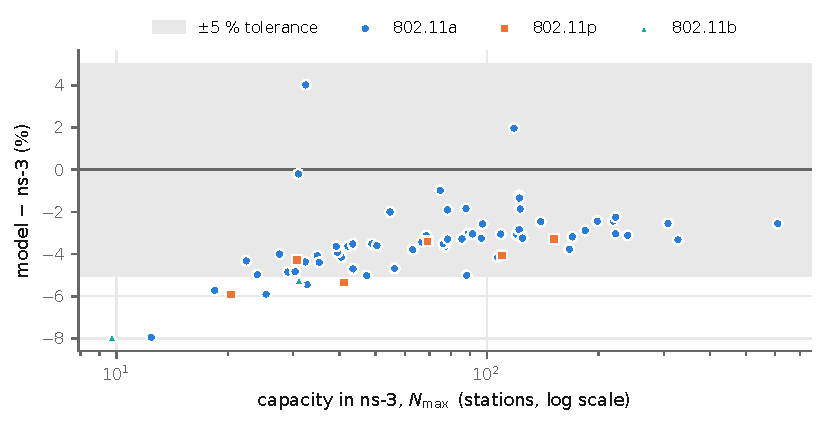
\includegraphics[width=\textwidth]{fig_scorecard}
\caption{The root of \eqref{eq:G5} against \scRows{} capacities stored from ns-3. Below zero, the
model under-predicts the capacity (the safe side).}
\label{fig:scorecard}
\end{figure}

\subsection{The safe side, by traffic source (UJ)}\label{sec:uj}

UJ tested on two new 802.11a cells whether the root of \eqref{eq:G5} stays on the safe side when the
stations' timers jitter or drift, and what frozen phases do (\cref{fig:uj}). It was registered with
two claims for the five non-frozen cells: S, the root at or below ns-3; A, the root and the law
within $\pm5\,\%$. \textbf{S held at all \ujSHeld{}}, the root's error \ujRootMax{} to \ujRootMin\,\%; A held at \ujAHeld, the two misses conservative. With frozen phases (strictly periodic senders,
identical clocks) ns-3's capacity fell by \ujFzDrop\,\% in both cells, to the root
(\ujFzRootMin{} and \ujFzRootMax\,\%) but not past it; the law, which lies slightly above the root,
was optimistic there (\ujFzLawMin{} to \ujFzLawMax\,\%). The registration's outcomes table sent that
case to Mohamed, who decided: \textbf{frozen phases are outside the safe-side claim}. The claim
the report makes is therefore: \emph{the root of \eqref{eq:G5} is on the safe side for timers with
jitter or clock drift} (all new cells, and all stored ones).

\begin{figure}[htbp]
\centering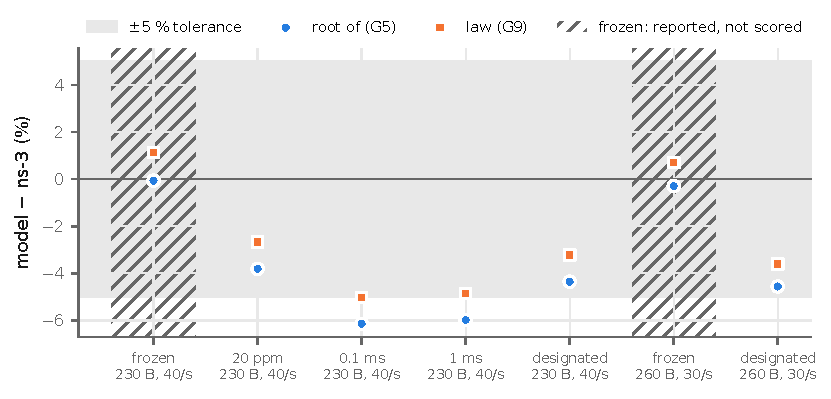
\includegraphics[width=\textwidth]{fig_uj}
\caption{UJ: the error of the root of \eqref{eq:G5} and of the law \eqref{eq:G9} against ns-3, by
traffic source, on two new 802.11a cells. Hatched: frozen phases, reported.}
\label{fig:uj}
\end{figure}

\iffull
\begin{table}[htbp]
\centering\footnotesize
% Generated by analysis/report_numbers.py from results/raw; do not edit by hand.
\begin{tabular}{lllrrllr}
\toprule
Cell & Source & ns-3 $\Nmax$ (95\,\% CI) & Root (\%) & Law (\%) & S & A & Seed $\sigma$ \\
\midrule
JA230F40 & frozen & 32.64 (30.85--33.77) & \textminus{}0.07 & +1.13 & reported & reported & 1.47 \\
JA230F40 & 20 ppm drift & 33.91 (31.64--34.43) & \textminus{}3.81 & \textminus{}2.66 & yes & yes & 1.61 \\
JA230F40 & jitter 0.1 ms & 34.75 (31.81--35.55) & \textminus{}6.14 & \textminus{}5.02 & yes & no & 1.46 \\
JA230F40 & jitter 1 ms & 34.69 (33.72--35.47) & \textminus{}5.98 & \textminus{}4.86 & yes & no & 1.19 \\
JA230F40 & designated & 34.10 (33.91--34.27) & \textminus{}4.36 & \textminus{}3.21 & yes & yes & 0.54 \\
JA260F30 & frozen & 40.09 (39.20--41.28) & \textminus{}0.30 & +0.70 & reported & reported & 1.47 \\
JA260F30 & designated & 41.88 (41.69--42.09) & \textminus{}4.56 & \textminus{}3.61 & yes & yes & 0.46 \\
\bottomrule
\end{tabular}

\caption{UJ in full (S: the root at or below ns-3; A: root and law within $\pm5\,\%$; seed $\sigma$:
the spread of each seed's own crossing).}
\end{table}
\fi

\subsection{The 802.11b arm, and why the sending pattern matters}

At the hardware's own PHY (802.11b, 1\,Mb/s), test UD found the Poisson model low at \udBelow{} of
its \udDOneAll{} small-swarm crossings. At 15--37 stations the root of \eqref{eq:G5} failed the
$\pm5\,\%$ band at \udDRootFailed{} of \udDCells{} cells, all on the safe side (\udDRootMax{} to
\udDRootMin\,\%); at 8--14 stations, with a band widened to $-9\ldots+5\,\%$ at registration, it held
at \udBHeld{} of \udBScored. Term by term, the loss itself was pessimistic by \udThreePMin{} to
\udThreePMax\,\% (D3); a capacity error is far smaller than a loss error because the loss rises
steeply with the load. The cause was the Poisson assumption: ns-3's telemetry source is periodic.
This failure is what \eqref{eq:G25} was written for.

\textbf{UD2 tested \eqref{eq:G25} where UD failed,} on new 802.11b cells at windows 8, 16 and 32 and
loss targets 2, 5 and 10\,\% (\cref{fig:ud2}). It held at all \udQHeld{} of \udQCrossings{}
crossings, with errors from \udQMin{} to \udQMax\,\%, including the \udQPast{} crossings past
occupancy 0.78. The Poisson root beside it erred by \udQPoiMin{} to \udQPoiMax\,\%, outside
$\pm5\,\%$ at \udQPoiOut: UD's failure, repeated on new cells and corrected by \eqref{eq:G25}. UD
itself stays failed as registered.

\begin{figure}[htbp]
\centering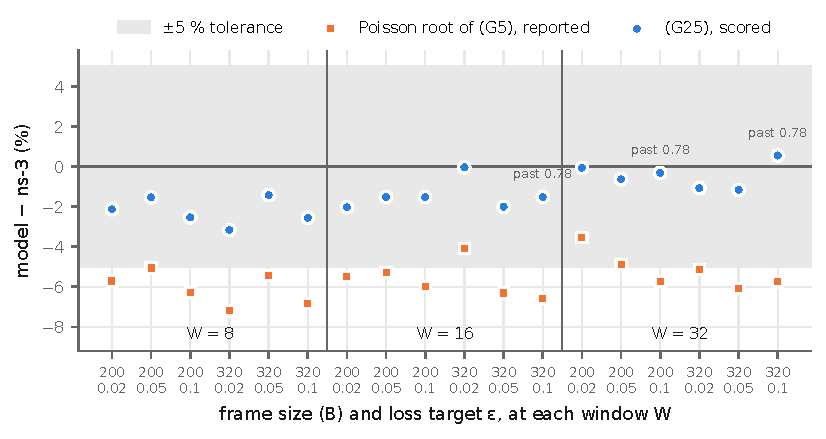
\includegraphics[width=\textwidth]{fig_ud2}
\caption{UD2: \eqref{eq:G25} (scored) and the Poisson root of \eqref{eq:G5} (reported) against
ns-3, 802.11b at 1\,Mb/s, two new frame sizes, three windows and three loss targets.}
\label{fig:ud2}
\end{figure}

\iffull
\begin{table}[htbp]
\centering\footnotesize
% Generated by analysis/report_numbers.py from results/raw; do not edit by hand.
\begin{tabular}{lrllrllr}
\toprule
Cell & $\Wnd$ & $\eps$ & ns-3 $\Nmax$ (95\,\% CI) & \eqref{eq:G25} & Error (\%) & Held & Poisson (\%) \\
\midrule
QB200F10W8 & 8 & 0.02 & 17.30 (17.11--17.44) & 16.93 & \textminus{}2.13 & yes & \textminus{}5.71 \\
QB200F10W8 & 8 & 0.05 & 24.82 (24.62--25.07) & 24.44 & \textminus{}1.54 & yes & \textminus{}5.06 \\
QB200F10W8 & 8 & 0.1 & 32.64 (32.46--32.81) & 31.81 & \textminus{}2.53 & yes & \textminus{}6.29 \\
QB320F8W8 & 8 & 0.02 & 15.47 (15.16--15.73) & 14.98 & \textminus{}3.16 & yes & \textminus{}7.20 \\
QB320F8W8 & 8 & 0.05 & 21.79 (21.60--22.06) & 21.48 & \textminus{}1.42 & yes & \textminus{}5.44 \\
QB320F8W8 & 8 & 0.1 & 28.60 (28.41--28.81) & 27.87 & \textminus{}2.55 & yes & \textminus{}6.82 \\
QB200F10W16 & 16 & 0.02 & 21.62 (21.33--22.08) & 21.18 & \textminus{}2.03 & yes & \textminus{}5.47 \\
QB200F10W16 & 16 & 0.05 & 30.10 (29.85--30.28) & 29.64 & \textminus{}1.51 & yes & \textminus{}5.28 \\
QB200F10W16 & 16 & 0.1 & 37.85 (37.69--38.05) & 37.27 & \textminus{}1.52 & yes & \textminus{}5.97 \\
QB320F8W16 & 16 & 0.02 & 18.82 (18.37--19.31) & 18.82 & \textminus{}0.03 & yes & \textminus{}4.07 \\
QB320F8W16 & 16 & 0.05 & 26.68 (26.50--26.88) & 26.15 & \textminus{}2.00 & yes & \textminus{}6.31 \\
QB320F8W16 & 16 & 0.1 & 33.26 (33.07--33.41) & 32.76 & \textminus{}1.51 (past 0.78) & yes & \textminus{}6.60 \\
QB200F10W32 & 32 & 0.02 & 25.66 (25.44--25.98) & 25.65 & \textminus{}0.06 & yes & \textminus{}3.55 \\
QB200F10W32 & 32 & 0.05 & 34.83 (34.64--35.06) & 34.61 & \textminus{}0.63 & yes & \textminus{}4.88 \\
QB200F10W32 & 32 & 0.1 & 42.16 (42.07--42.23) & 42.03 & \textminus{}0.30 (past 0.78) & yes & \textminus{}5.72 \\
QB320F8W32 & 32 & 0.02 & 23.21 (22.82--23.45) & 22.96 & \textminus{}1.07 & yes & \textminus{}5.13 \\
QB320F8W32 & 32 & 0.05 & 31.07 (30.82--31.26) & 30.71 & \textminus{}1.16 & yes & \textminus{}6.08 \\
QB320F8W32 & 32 & 0.1 & 36.92 (36.81--37.08) & 37.13 & +0.56 (past 0.78) & yes & \textminus{}5.75 \\
\bottomrule
\end{tabular}

\caption{UD2 in full, scored at $\pm5\,\%$.}
\end{table}
\fi

\subsection{The sending pattern}

With Poisson sources the model is \ugPoiMin{} to \ugPoiMax\,\% low on the new cells of UG25.
\eqref{eq:G25} was registered on those \ugCells{} cells and held at all \ugHeld{} (\ugMin{} to
\ugMax\,\%). Past occupancy 0.78 (\uhCells{} further cells at occupancy \uhOccMin--\uhOccMax) it is
optimistic by \uhMin{} to \uhMax\,\%, which is now a stated limit (\cref{fig:g25}).

\begin{figure}[htbp]
\centering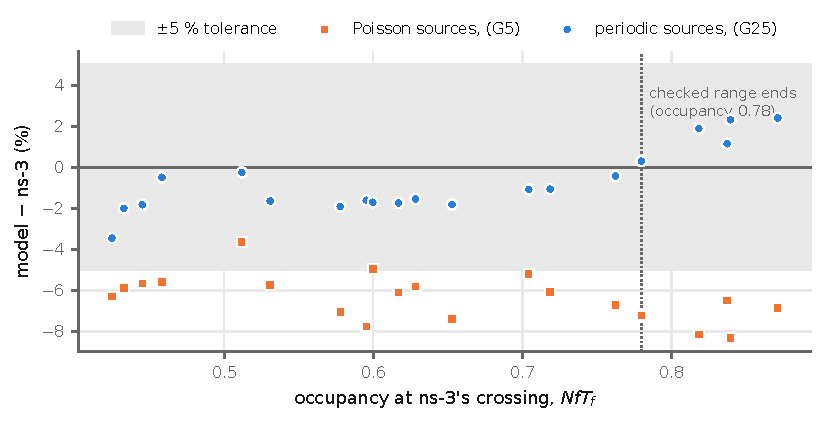
\includegraphics[width=\textwidth]{fig_g25}
\caption{The model's error against ns-3, with Poisson sources, \eqref{eq:G5}, and with periodic
sources, \eqref{eq:G25}, against the occupancy at which ns-3 reaches the loss target.}
\label{fig:g25}
\end{figure}

\subsection{Few stations}

For three to five stations the finite-station form \eqref{eq:FS} held at all \fsHeld{} of \fsCells{}
registered cells, with a tolerance of $\pm15\,\%$ on the loss (\cref{fig:fewstations}). The Poisson
loss \eqref{eq:G5} overstates the loss there by \fsGFiveMin--\fsGFiveMax\,\%.

\begin{figure}[htbp]
\centering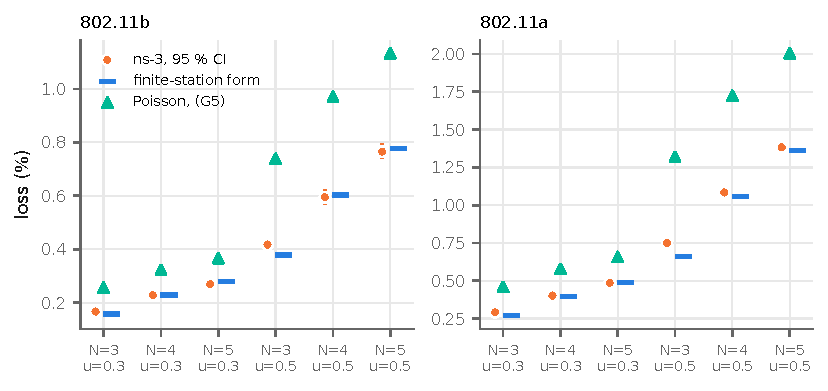
\includegraphics[width=\textwidth]{fig_fewstations}
\caption{UFS: the loss at three to five stations and occupancy 0.3 and 0.5, in ns-3 (30 seeds, 95\,\%
interval), by the finite-station form \eqref{eq:FS} and by the Poisson loss \eqref{eq:G5}.}
\label{fig:fewstations}
\end{figure}

\subsection{Batching}

The gain of batching \eqref{eq:G12} matched ns-3 within \gainMaxAbs\,\% at 802.11a up to 64 records
per frame, and within \gainBMaxAbs\,\% at 802.11b up to 32 (\cref{fig:batching}; reported beside
registered capacity tests UC2 and UD, whose capacities held \ucTwoHeld{} of \ucTwoClaims{} and
\udTwoHeld{} of \udTwoCells).

\begin{figure}[htbp]
\centering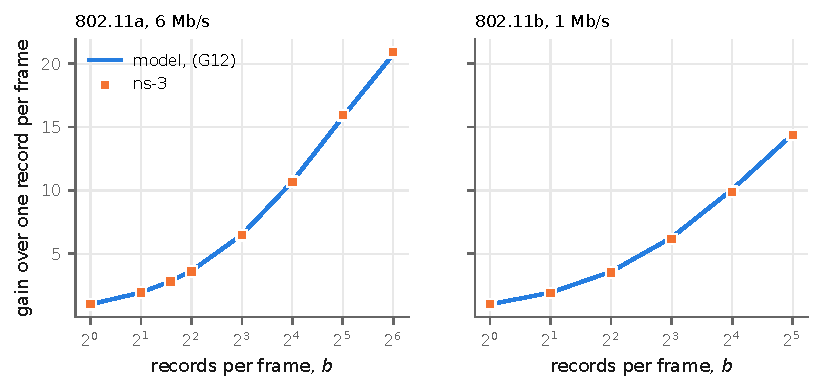
\includegraphics[width=\textwidth]{fig_batching}
\caption{The gain of batching: capacity at $b$ records per frame over capacity at one, less one
station each, \eqref{eq:G12} against ns-3.}
\label{fig:batching}
\end{figure}

\subsection{Capture}

ns-3's capture rule, read from its source and predicted per collision, held at \capHeld{} of
\capTrials{} offsets and power differences (UCAP2). A first capacity test with capture (UF) held
\ufAvgHeld{} of \ufConfigs{} average-delivery claims and only \ufWorstHeld{} of \ufConfigs{}
every-sender claims. Its three causes were found: the half-duplex factor \eqref{eq:G22a} was missing,
the every-sender claim had been scored on a sample minimum rather than on \eqref{eq:G24} or
\eqref{eq:G24a}, and one configuration had a station at the edge of carrier sense. The corrected
test UF2, on new placements and seeds, held all \ufTwoHeld{} of its \ufTwoClaims{} claims, every one
on the safe side: \eqref{eq:G23} within \ufTwoAMin{} to \ufTwoAMax\,\%, the pooled \eqref{eq:G24}
within \ufTwoPoolMin{} to \ufTwoPoolMax\,\%, the window statistic \eqref{eq:G24a} within
\ufTwoWinMin{} to \ufTwoWinMax\,\% (\cref{fig:uf2}).

\begin{figure}[htbp]
\centering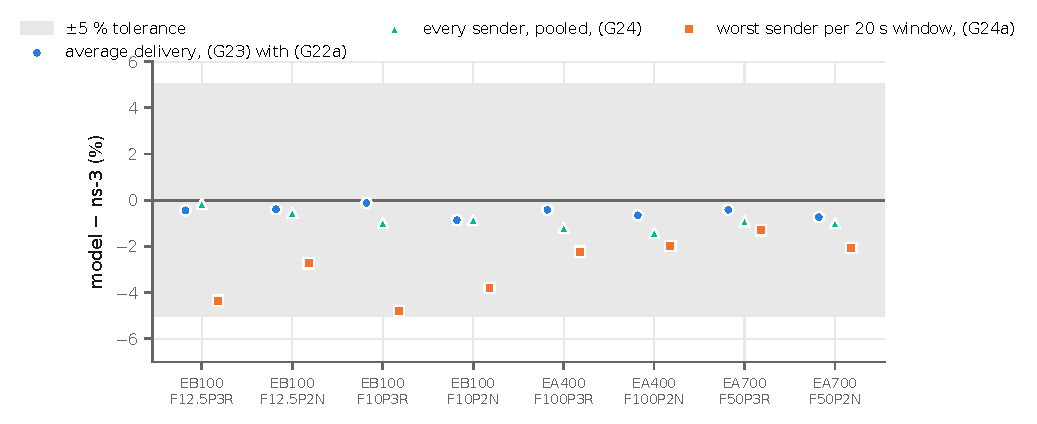
\includegraphics[width=\textwidth]{fig_uf2}
\caption{UF2: the capture laws against ns-3, per configuration (EB: 802.11b, EA: 802.11a; F: frames
per second; P3R: path-loss exponent 3 with Rayleigh fading; P2N: exponent 2, no fading).}
\label{fig:uf2}
\end{figure}

\subsection{Design rules and LoRa}

A key record once in $r=2$ or 4 frames held \ucThreeHeld{} of \ucThreeCells{} (UC3). Fragments spread
over the period held \ucFourSHeld{} of \ucFourSCells{} (UC4S); fragments sent back to back failed
(UC4), and a correction for them removed \burstFixMin--\burstFixMax\,\% of the excess but failed its
own test (UC4B), so the design forbids back-to-back fragments. The best batch under bit errors
\eqref{eq:G19} was predicted as \ucFivePred{} and ns-3's best was \ucFiveBest{} (UC5D1). The LoRa
duty-cycle law held at \lrHeld{} of \lrCells{} cells (UC7).

\subsection{What failed in simulation}

\begin{itemize}
\item \textbf{The split of \eqref{eq:G5} into its three causes} (UC1, D3): the totals hold, the
breakdown does not; ns-3 counts a near-simultaneous start as a detection-window loss.
\item \textbf{Poisson starts at 802.11b} (UD): the capacity \udDRootMax{} to \udDRootMin\,\% low at
15--37 stations; \eqref{eq:G25} then held at all \udQCrossings{} new crossings of UD2.
\item \textbf{The first capture test} (UF): failed for three identified reasons; the corrected test
held on new cells.
\item \textbf{Fragments sent back to back} (UC4, UC4B): outside the model; ruled out by design.
\item \textbf{\eqref{eq:G25} past occupancy 0.78 at 802.11b}: optimistic by \uhMin{} to \uhMax\,\%;
a stated limit.
\item \textbf{Frozen phases} (UJ and the stored cells): ns-3's capacity falls by about
\ujFzDrop\,\%, to the root or past it, and the law is optimistic there (stored: \scLawOptErr\,\%);
excluded from the safe-side claim.
\end{itemize}

% ==================================================================================================
\section{Validation on hardware}\label{sec:hw}
% ==================================================================================================

\textbf{What the hardware tests checked.} W1e, W1j and W1k were registered before the closed form
existed. Their predictions came from the project's event simulation of the DCF access rule
(registered at W1c), which had matched ns-3's capacities at 802.11b within \wOneBErr\,\% (W1b). They test
the access-rule model the closed form is built on, not the closed form's own numbers. W1r's
registration also recorded the closed form's values beside ns-3's; they are compared in
\cref{sec:side}. The first test of the closed form itself on the radios is V1a, below.

\subsection{The closed form on the radios (V1a)}\label{sec:v1a}

On three radios the part of the closed form that applies is the few-station form \eqref{eq:FS}
(three to five stations, occupancy up to 0.5). V1a scored it \emph{as stated}: the standard's window
$\Wnd=32$, rule set A, nothing measured on the radios. The three radios sent at occupancy 0.3, 0.4
and 0.5 in five interleaved rounds, with a control window after each; the session ran remotely and
every validity condition held (background \vaBg\,\%, each radio's link loss alone at most
\vaLinkMax\,\%). The registered tolerance was $\pm15\,\%$ on the loss.

\textbf{The closed form as stated failed at all \vaPoints{} points, on the optimistic side}
(\cref{fig:v1a,tab:v1a}). The radios lost \vaFacMin--\vaFacMax{} times what \eqref{eq:FS} predicts,
and the form lies below the 95\,\% interval of the measurement at every point. ns-3 and the event
simulation, both with the standard rule, sit near the form: the radios lose \vaSimMin--\vaSimMax{}
times what they predict. What misses is therefore the access rule the model assumes, not the
closed form's approximation of that rule. C1 measured the likely cause: the Pi~4s send about half
their frames at DIFS with no backoff, and the Pi~3 waits a fixed \cExtraC\,\us{} longer. A
hardware-matched form, with the radios' measured rule as its input, is the next registered test
(V1b, \cref{sec:next}). The failure was expected and disclosed in the registration; the stored trio
point of W1e and W1r had already pointed to it.

\begin{figure}[htbp]
\centering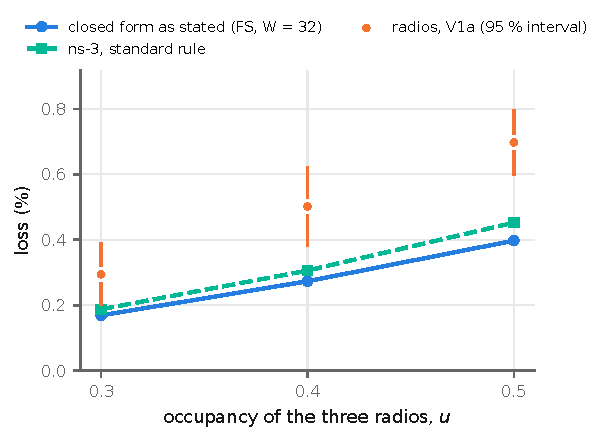
\includegraphics[width=0.66\textwidth]{fig_v1a}
\caption{V1a: the loss of the three radios against the closed form as stated, \eqref{eq:FS} at
$\Wnd=32$, and ns-3 with the standard rule.}
\label{fig:v1a}
\end{figure}

\begin{table}[htbp]
\centering\small
% Generated by analysis/report_numbers.py from results/raw; do not edit by hand.
\begin{tabular}{rrlrrlrrr}
\toprule
$\occ$ & $f$ & Radios, \% (95\,\% CI) & \eqref{eq:FS}, \% & Error (\%) & Held & ns-3, \% & Event sim., \% & \eqref{eq:G5}, \% \\
\midrule
0.3 & 52 & 0.294 (0.198--0.391) & \textbf{0.169} & \textminus{}42.7 & \textbf{no} & 0.188 & 0.193 & 0.263 \\
0.4 & 70 & 0.501 (0.378--0.625) & \textbf{0.273} & \textminus{}45.5 & \textbf{no} & 0.306 & 0.312 & 0.468 \\
0.5 & 87 & 0.697 (0.597--0.798) & \textbf{0.397} & \textminus{}43.0 & \textbf{no} & 0.452 & 0.446 & 0.743 \\
\bottomrule
\end{tabular}

\caption{V1a, scored at $\pm15\,\%$. The last three columns were reported, not scored;
\eqref{eq:G5} lies outside its stated range at three stations. Its closeness to the radios
(\vaGfiveMin{} to \vaGfiveMax\,\%) is not evidence for it: periodic sources make it pessimistic for
three stations, while the radios' rule adds collisions, so two departures act in opposite
directions; the matched form will separate them.}
\label{tab:v1a}
\end{table}

\subsection{Contention}

\Cref{fig:hw} shows the loss of two and three radios at occupancy 0.50, 0.70 and 0.85. In W1e (frame
burst on) \weHeld{} of \wePoints{} points lay inside the bands registered from the event
simulation; the miss was pi-A with pi-B at the lowest load, \weMissRatio{} times the prediction against a band
top of \weMissTop. In W1r (frame burst off) the hardware lies between two ns-3 settings of slot and
DIFS: inside the 95\,\% interval at \wrInTwenty{} of \wrPoints{} points for slot 20\,\us/DIFS
50\,\us, and \wrInNine{} for slot 9\,\us/DIFS 28\,\us. The pairs with the Pi 3 lose more than ns-3
predicts; ns-3 had been given windows inferred from each radio's sending rate, $\Wnd=\wrWinPi$ for
the Pi 4s and \wrWinPiThree{} for the Pi 3, and C1 later showed both to be wrong in kind
(\cref{sec:window}).

\begin{figure}[htbp]
\centering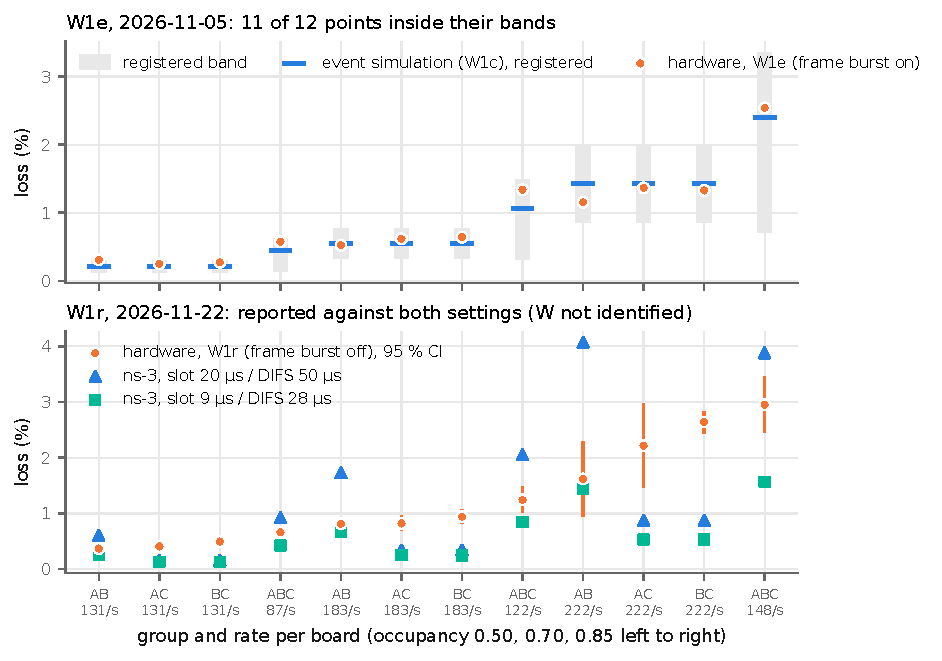
\includegraphics[width=\textwidth]{fig_hw_contention}
\caption{Hardware contention. Top: W1e against its registered prediction (the event simulation of
W1c). Bottom: W1r against ns-3 with two settings of slot and DIFS (the contention window was not
known; \cref{sec:window}).}
\label{fig:hw}
\end{figure}

\subsection{The capacity ratio}

On four radios (pi-A, pi-B, the Pi 3 and the TP-Link), the capacity of the design (one signature per
frame of four records) divided by that of per-record signing was \ratioJ{} in W1j and \ratioK{} in
W1k, against the registered \ratioModel{} (band \ratioLo--\ratioHi; \cref{fig:ratio}). The capacities
themselves were \crossAuthJ{} and \crossPerJ{} capacity-equivalent stations in W1j, against
\crossAuthModel{} and \crossPerModel{} (\crossAuthErr{} and \crossPerErr\,\%), attributed in W1j
to capture at the receivers, while the ratio moved by \ratioErr\,\%.

\begin{figure}[htbp]
\centering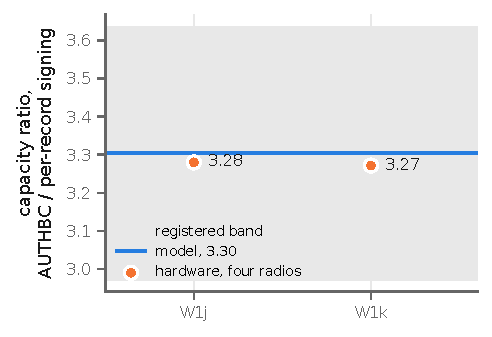
\includegraphics[width=0.5\textwidth]{fig_ratio}
\caption{The capacity ratio on four radios against the registered value.}
\label{fig:ratio}
\end{figure}

\subsection{Loss on air}

W3a traced every frame on air at 802.11b and replayed the traces through the project's real
decoder. All \wtHeld{} of \wtClaims{} registered claims held: real loss hurts the frames that depend
on a key record no more than independent loss would; the design loses only its own frames; and the
loss grows with frame length less steeply than a bit-error model predicts.

\subsection{Capture}

In W1q (the Pi 3 receiving, pi-A's power stepped) \wqHeld{} of \wqScored{} registered predictions
held. The one that failed is the finding: at a measured difference of only \wqThreeDelta\,dB the Pi
3 kept the stronger frame in \wqThreeQ{} of collisions, where ns-3's rule keeps none below 4\,dB.
Capture on this radio is gradual, not a step. Three of W1q's five power steps were void because the
received signal fell by less than the set power (\cref{sec:window}). W1s then tested the gradual
curve on new power steps: \wsCurveHeld{} of \wsCurveScored{} held, so the curve is not used; the
boards' radio geometry had changed between the sessions (\cref{fig:capture}).

\begin{figure}[htbp]
\centering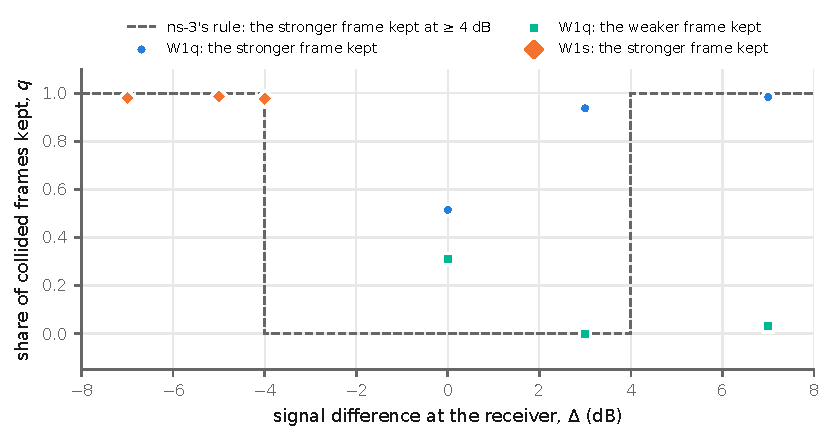
\includegraphics[width=\textwidth]{fig_capture_hw}
\caption{The share of collided frames the receiver kept, against the signal difference. Dashed:
ns-3's 4\,dB rule. W1q's points are from its valid steps; W1s's from its new steps.}
\label{fig:capture}
\end{figure}

\subsection{The contention window, and the radios' own timing}\label{sec:window}

The model needs each radio's contention window $\Wnd$, slot and DIFS; radios do not report them.
\textbf{W1p} tested two settings derived from each radio's sending rate: a saturated pair lost
\wpLoss{} at \wpFps{} frames/s, against ns-3's \wpTwentyLoss{} and \wpNineLoss: neither fits.
\textbf{W1s} re-derived both settings once and tested them at a new frame length: the pair lost
\wsPairLoss{} at \wsPairFps{} frames/s, against \wsTwentyLoss{} and \wsNineLoss: neither fits again,
so the window is recorded as not identifiable without a frame sniffer.

A sniffer was therefore added (the TP-Link in monitor mode, with a one-line driver change that
exports the chip's per-frame hardware timestamp). Its gate S0 \textbf{failed}: it recorded \sgA,
\sgB{} and \sgC{} of the three radios' frames, against the 0.99 required, though the radios
themselves received almost all of them; the misses follow neither the board nor its place, and a
probe at another placement (P1) did not reach 0.99 either; its planned placements 3\,m and 5\,m
away have not run. The same gate showed that the received signal
falls by \sgFalls\,dB when pi-A's set power falls by 3, 6 and 9\,dB; the Pi 3 registered a similar
compression, so the transmitter is the more likely cause, but this is not established. The sniffer
is used for timing only, under a stated rule, until a better adapter arrives.

\textbf{C1 (calibration, not validation)} measured each radio alone with the sniffer's microsecond
timestamps (\cref{fig:c1}). For both Pi 4s the gap after a frame has a floor of \cFloorA\,\us{} (the
standard's DIFS) and a 20\,\us{} lattice (the standard's slot); \cShareMinA--\cShareMaxB{} of their
frames are sent at DIFS with no backoff, and the rest spread over \cWminA{} slots. Under the
standard's rule a saturated sender draws its backoff from $0\ldots\Wnd-1$ after every frame, so only
about $1/\Wnd$ of frames (3\,\% at $\Wnd=32$) would go out at DIFS. Departures of commercial 802.11b cards from the standard's backoff have been
measured before \cite{bianchi2007cards}. The share did not change with a
back-to-back sender (\cShareKA), so it is the radio's own behaviour, not the sending pattern. The
Pi 3's floor is \cFloorC\,\us{} (\cExtraC\,\us{} more than DIFS) and \cShareMinC--\cShareMaxC{} of its
frames skip the backoff, close to the standard's $1/\Wnd$, with \cWminC--\cWmaxC{} slots. Across
frame sizes the airtime grows by \cSlope\,\us{} per byte (1\,Mb/s), with an intercept of
\cInterA\,\us{} (the long preamble, 192\,\us, plus DIFS). These are inputs for a hardware-matched
model; nothing has yet been validated with them.

\begin{figure}[htbp]
\centering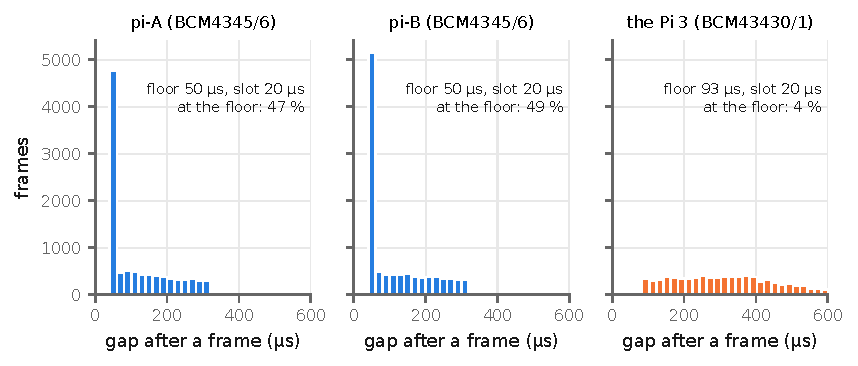
\includegraphics[width=\textwidth]{fig_c1_gaps}
\caption{C1: the gap after each frame, for each radio sending alone (145\,B frames). One bin per
backoff slot.}
\label{fig:c1}
\end{figure}

\iffull
\begin{figure}[htbp]
\centering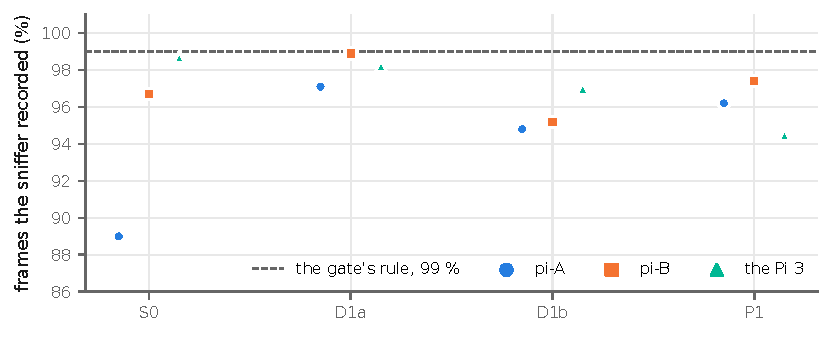
\includegraphics[width=\textwidth]{fig_sniffer}
\caption{The share of each radio's frames the sniffer recorded, session by session (S0: the gate;
D1a, D1b: diagnostics, pi-A and pi-B swapped in D1b; P1: the probe). The misses follow neither the
board nor its place.}
\label{fig:sniffer}
\end{figure}
\fi

\subsection{What failed on hardware}

\begin{itemize}
\item \textbf{The closed form as stated} (V1a): \eqref{eq:FS} at $\Wnd=32$ lies \vaErrB{} to
\vaErrA\,\% from the radios' loss at occupancy 0.3--0.5; the standard access rule is what differs.
\item \textbf{The window, from sending rates} (W1p, W1s): neither setting of slot and DIFS fits; the
window was not identifiable that way. C1 shows why: the Pi 4s skip the backoff for about half their
frames, which no single window describes.
\item \textbf{ns-3's 4\,dB capture step} (W1q): the radio captures at 1.5\,dB; the gradual curve
then failed its own check on new steps (W1s) after the geometry changed.
\item \textbf{The sniffer's gate} (S0, P1): the adapter misses \snifMissMin--\snifMissMax\,\% of frames, drifting between
sessions.
\item \textbf{Power steps}: the received signal falls by less than the set power, most likely at the
transmitter.
\end{itemize}

% ==================================================================================================
\section{Model, simulation and hardware side by side}\label{sec:side}
% ==================================================================================================

\Cref{tab:threeway} puts every source of a prediction beside the two hardware sessions, for the same
radios and rates: the closed forms (as recorded in W1r's registration, at the standard's
$\Wnd=32$), W1c's event simulation (W1e's registered prediction), ns-3 with two settings of slot and
DIFS, and the hardware with frame burst on (W1e) and off (W1r).

\begin{table}[htbp]
\centering\footnotesize
% Generated by analysis/report_numbers.py from results/raw; do not edit by hand.
\begin{tabular}{lrrrrrrrrrr}
\toprule
Radios & $\occ$ & $f$ & \eqref{eq:G5} & \eqref{eq:G25} & Finite & Event model & ns-3, $\slot=20$ & ns-3, $\slot=9$ & W1e & W1r \\
\midrule
AB & 0.50 & 131 & 0.41 & 0.30 & -- & 0.22 & 0.60 & 0.25 & 0.31 & 0.37 \\
AC & 0.50 & 131 & 0.41 & 0.30 & -- & 0.22 & 0.16 & 0.13 & 0.25 & 0.41 \\
BC & 0.50 & 131 & 0.41 & 0.30 & -- & 0.22 & 0.16 & 0.13 & 0.27 & 0.50 \\
ABC & 0.50 & 87 & 0.74 & 0.55 & 0.40 & 0.45 & 0.92 & 0.42 & 0.58 & 0.66 \\
AB & 0.70 & 183 & 0.83 & 0.54 & -- & 0.55 & 1.73 & 0.67 & 0.52 & 0.81 \\
AC & 0.70 & 183 & 0.83 & 0.54 & -- & 0.55 & 0.34 & 0.25 & 0.62 & 0.82 \\
BC & 0.70 & 183 & 0.83 & 0.54 & -- & 0.55 & 0.34 & 0.24 & 0.64 & 0.94 \\
ABC & 0.70 & 122 & 1.66 & 1.10 & -- & 1.06 & 2.05 & 0.84 & 1.34 & 1.24 \\
AB & 0.85 & 222 & 1.31 & 0.79 & -- & 1.43 & 4.07 & 1.44 & 1.15 & 1.62 \\
AC & 0.85 & 222 & 1.31 & 0.79 & -- & 1.43 & 0.87 & 0.53 & 1.37 & 2.21 \\
BC & 0.85 & 222 & 1.31 & 0.79 & -- & 1.43 & 0.87 & 0.53 & 1.33 & 2.64 \\
ABC & 0.85 & 148 & 2.82 & 1.69 & -- & 2.40 & 3.88 & 1.57 & 2.54 & 2.95 \\
\bottomrule
\end{tabular}

\caption{Loss (\%) of two and three radios, 802.11b at 1\,Mb/s, $f$ frames per second per radio.
For the pairs, \eqref{eq:G5} and \eqref{eq:G25} lie outside their stated range (two stations;
\eqref{eq:G25} needs 8 or more others); the finite-station form is shown only where it was accepted
(three stations, occupancy 0.5). The ns-3 values for the pairs with the Pi 3 use its inferred window
of \wrWinPiThree{} slots.}
\label{tab:threeway}
\end{table}

\textbf{What the comparison shows.}
\begin{itemize}
\item \textbf{The trio at occupancy 0.5}, the one point inside every model's range: \eqref{eq:FS},
the event simulation, ns-3 at slot 9\,\us{} and both hardware sessions lie between \twTrioLo{} and
\twTrioHi\,\%; \eqref{eq:G5} and ns-3 at slot 20\,\us{} lie above them.
\item \textbf{The pairs:} no closed form is claimed for two stations. ns-3's values for the pairs
with the Pi 3 are \twPiThreeLo--\twPiThreeHi{} times below the hardware, because ns-3 was given a window of
\wrWinPiThree{} slots for the Pi 3; C1 measured \cWminC--\cWmaxC{} plus a fixed \cExtraC\,\us.
\item \textbf{The same radios, two sessions} (W1e and W1r) differ by up to a factor of \twSessMax{} for the
pairs with the Pi 3: frame burst, placement and day all changed between them. A hardware number is a
property of a session, not only of the radios.
\end{itemize}

\begin{table}[htbp]
\centering\small
\begin{tabularx}{\textwidth}{>{\raggedright\arraybackslash}p{3.9cm}>{\raggedright\arraybackslash}p{2.4cm}>{\raggedright\arraybackslash}p{2.4cm}L}
\toprule
Quantity & Model & ns-3 & Hardware \\
\midrule
loss of three radios at $\occ=0.5$ (V1a) & \vaFinC\,\% \eqref{eq:FS} & \vaNsC\,\% (standard rule) & \vaLossC\,\% \\
capacity ratio, design over per-record signing (4 radios) & \ratioModel{} (event simulation) & -- & \ratioJ, \ratioK{} (W1j, W1k) \\
gain of batching, 802.11a, $b$ up to 64 & \eqref{eq:G12} & within \gainMaxAbs\,\% & not tested (V2) \\
capture at a signal difference of \wqThreeDelta\,dB & \eqref{eq:G22} with the input $q$ & $q=0$ (4\,dB rule) & $q=\wqThreeQ$ (W1q) \\
slot, DIFS & 20\,\us, 50\,\us{} (standard) & the same & 20\,\us, \cFloorA\,\us{} (Pi 4s); 20\,\us, \cFloorC\,\us{} floor (Pi 3) \\
frames sent at DIFS with no backoff, saturated & about $1/\Wnd$ (the standard's backoff after every frame) & not measured & \cShareMinA--\cShareMaxB{} (Pi 4s); \cShareMinC--\cShareMaxC{} (Pi 3) \\
airtime per byte at 1\,Mb/s & 8\,\us & 8\,\us & \cSlope\,\us{} (C1) \\
\bottomrule
\end{tabularx}
\caption{One quantity at a time: what the model assumes or predicts, what ns-3 does, what the radios
do.}
\label{tab:side}
\end{table}

% ==================================================================================================
\section{What remains to be tested}\label{sec:next}
% ==================================================================================================

\Cref{tab:coverage} maps each part of the model against where it has been tested.
\Cref{tab:next} lists the open tests, in the order they can run.

\begin{table}[htbp]
\centering\small
\begin{tabularx}{\textwidth}{>{\raggedright\arraybackslash}p{4.2cm}LL}
\toprule
Part of the model & ns-3 & Hardware \\
\midrule
accounting and batching, \eqref{eq:G1}--\eqref{eq:G3}, \eqref{eq:G10}--\eqref{eq:G13} & held (UC2, UD) & ratio held (W1j, W1k, event simulation); gain on air not tested (V2) \\
loss \eqref{eq:G4}--\eqref{eq:G5} & total held; split into causes failed (UC1) & as stated, \textbf{failed} (V1a, through \eqref{eq:FS}); the radios' access rule differs (C1) \\
two-constant law \eqref{eq:G6}--\eqref{eq:G9} & held where valid, \scLawIn{} of \scLawRows & not tested \\
design rules \eqref{eq:G16}--\eqref{eq:G21} & held (UC3, UC4S, UC5D1, UC7); back-to-back fragments failed & not tested \\
capture \eqref{eq:G22}--\eqref{eq:G24a} & held after correction (UCAP2, UF2) & the input $q$ measured, partly (W1q); in contention not tested (V3, V4) \\
sending pattern \eqref{eq:G25}, \eqref{eq:FS} & held to occupancy 0.78, and at 802.11b at every window and target (UD2); 3--5 stations held & \eqref{eq:FS} as stated \textbf{failed} (V1a); with the measured rule: V1b \\
hidden stations; two stations & not tested; no closed form & not tested \\
\bottomrule
\end{tabularx}
\caption{The coverage map: where each part of the model has been tested, and how it came out.}
\label{tab:coverage}
\end{table}

\begin{table}[htbp]
\centering\small
\begin{tabularx}{\textwidth}{>{\raggedright\arraybackslash}p{3.6cm}>{\raggedright\arraybackslash}p{1.9cm}L>{\raggedright\arraybackslash}p{2.9cm}}
\toprule
Test & Where & What it would show & Waits on \\
\midrule
S0b: the AR9271 sniffer's gate, beside the TP-Link & hardware & whether a second sniffer records $\ge99\,\%$ of frames; whether the power steps compress at the sender & the adapter (by 30 November 2026) \\
C1 in W1q's layout (L1); P1 at 3\,m and 5\,m & hardware & the timing of C1 where the capture sessions ran; whether distance lets the TP-Link reach 0.99 & Mohamed at the boards \\
C2: saturated pairs with the sniffer & hardware & the access rule two radios use under contention: who skips the backoff, and when & S0b \\
C3: the capture curve, both signs of the signal difference & hardware & $q$ against the signal difference for the real receiver & S0b \\
The parameter file & -- & the measured slot, DIFS, access rule, airtime and link losses, as one input set & C1--C3; Mohamed's review \\
The hardware-matched form: \eqref{eq:FS} with each radio's measured backoff and fixed delay, checked against the event simulation & model & the closed form with the radios' own rule, derived and checked before any test & Mohamed's acceptance of the derivation \\
V1b: the matched form on a new session of the three radios, as V1a & hardware & whether the closed form predicts the radios once it is given their rule & C2; the parameter file \\
V2: batching on air & hardware & the gain \eqref{eq:G12} on real radios & the parameter file \\
V3, V4: capture in contention; every-sender statistics & hardware & \eqref{eq:G22}--\eqref{eq:G24a} on real radios & C3 \\
Transmitter or receiver: does pi-A's output follow its set power? & hardware & where the power steps compress & an external receiver (HackRF) if S0b cannot separate them \\
Hidden stations & ns-3 & the term $2h\nu\Tf$ & outside the current scope \\
Two stations; fragments sent back to back & model & a closed form (none exists) & a derivation \\
\bottomrule
\end{tabularx}
\caption{The open tests. Calibration (C) sets the inputs; validation (V) tests predictions made from
them; no session does both.}
\label{tab:next}
\end{table}

If no suitable adapter is available by 30 November 2026, C2 and C3 use the receivers' logs, as W1p
and W1q did, with the sniffer for timing only, and the report of those sessions states the
limitation.

% ==================================================================================================
\section{Conclusions}
% ==================================================================================================

\begin{itemize}
\item \textbf{What can be claimed now.} The closed form predicts ns-3's capacity within $\pm5\,\%$ in
\scRootIn{} of \scRows{} stored cases, and its root lies on the safe side for every timer with jitter
or clock drift (UJ); frozen phases are excluded. Its extensions
for the sending pattern and for capture hold in registered ns-3 tests on new cells. On hardware, the
capacity ratio of the design over per-record signing matches the registered value (\ratioJ{}
against \ratioModel), and the access-rule model behind the closed form fell inside the registered
bands at \weHeld{} of \wePoints{} contention points.
\item \textbf{What cannot be claimed yet.} That the closed form predicts the radios' loss: as stated,
with the standard's access rule, it does not (V1a: the radios lose \vaFacMin--\vaFacMax{} times its
prediction, and ns-3 with the same rule misses alike); whether it does with the radios' measured
rule is the next test (V1b). That the model's access rule is the radios': the Pi 4s send about
half their frames with no backoff, which the standard's rule does not include. That ns-3's 4\,dB
capture step describes the real receiver: it captures gradually.
\item \textbf{Next.} The hardware-matched form (derived, then checked against the event simulation);
a sniffer that passes its gate and the calibration sessions C2 and C3; the parameter file for
review; then V1b and the validation sessions V2--V4 against the matched model and ns-3.
\end{itemize}

\iffull
\appendix
% ==================================================================================================
\section{Notation}
% ==================================================================================================
\begin{table}[htbp]
\centering\small
\begin{tabular}{ll}
\toprule
Symbol & Meaning \\
\midrule
$\Lam$ & records per second per station \\
$b$, $\bstar$, $\bM$ & batch (records per frame); the batch used; the largest that fits \\
$\Dmax$, $\Dnet$, $\Sq$ & deadline; deadline net of the delay $\Sq$ \\
$\Phi$, $\Psi$, $\Bud$ & cost per frame, cost per record, budget of a resource \\
$\Tf$ & a frame's airtime \\
$f$, $\nu$ & frames per second per station; start rate of the other stations, $(N-1)f$ \\
$\occ$ & occupancy, $N f\Tf$ \\
$\slot$, $\Difs$, $\Wnd$, $\delta$ & slot, DIFS, contention window, preamble-detection time \\
$\eps$, $\eps'$, $\epsw$ & loss target; with capture, average; with capture, every sender \\
$\rhostar$, $\tauzero$, $\tauhat$, $\kappa$ & the two constants of \eqref{eq:G9}; per-frame channel cost; $1-\eps/2$ \\
$\Kbar$, $a$, $\gamma$, $\eta$ & co-waiting frames; busy, gap and immediate-access loads \\
$\pcoll$, $q$, $\qeff$, $\ell$, $\ellbar$ & collision loss; capture probability; with the half-duplex factor; link loss; its average \\
$\Ninf$, $\beta$, $\Gain$ & capacity limit, half-gain batch, gain of batching \\
$\Rper$ & periodic-source ratio of \eqref{eq:G25} \\
$m$, $M$, $\pi$ & bystanders, co-waiting count and co-waiting probability of \eqref{eq:FS} \\
$z_N$ & expected maximum of $N$ standard normal draws \\
\bottomrule
\end{tabular}
\end{table}

% ==================================================================================================
\section{Failed attempts and corrections, kept visible}
% ==================================================================================================

\begin{itemize}
\item \textbf{UF (capture, first test).} \ufAvgHeld{} of \ufConfigs{} and \ufWorstHeld{} of
\ufConfigs{} held. Three causes, each found from logged state, not assumed: the half-duplex factor
\eqref{eq:G22a} had been omitted from both the law and its check script, so their agreement could not
reveal it; the every-sender claim had been scored on a sample minimum, an extreme that grows with
the number of senders, rather than on \eqref{eq:G24} or \eqref{eq:G24a}; one configuration placed a
station at the edge of carrier sense, outside one collision domain. UF stays failed; UF2 tested the
corrections on new placements and seeds.
\item \textbf{UC4B (a burst correction for back-to-back fragments).} Removed
\burstFixMin--\burstFixMax\,\% of the excess but failed on both scored cells, on the optimistic
side. Not used; the design rule forbids the case.
\item \textbf{UG25H: \eqref{eq:G25} at high occupancy.} An earlier estimate from capture runs put
the error at \fOneFortyMin--\fOneFortyMax\,\%; measured once without capture it is \uhMin{} to \uhMax\,\%. The band of
the earlier estimate held at none of the four cells.
\item \textbf{W1p and W1s (the window from sending rates).} Two re-derivations, two failures; by
Mohamed's rule no third attempt was made, and the window was recorded as not identifiable without a
sniffer.
\item \textbf{W1q's gradual capture curve.} Fitted after W1q's failure, then checked on new steps in
W1s: \wsCurveHeld{} of \wsCurveScored{}; not used.
\item \textbf{S0's timing criterion.} The registration compared the median of the sniffer's
start-to-start intervals with the receivers' mean cycle; with half the gaps at DIFS the median was
bound to fall below the mean. The means agree within \sZeroMeanMin--\sZeroMeanMax\,\%. A corrected gate (S0b) compares
mean with mean on new windows.
\item \textbf{C1's estimators.} Two estimators were revised after the gate's rate checks and before
C1 ran (the lattice had picked a harmonic; $\Wnd-1$ from a percentile read the long tail); both were
tested on synthetic gaps of known slot and window first, and the revision is disclosed in C1's
registration.
\end{itemize}

\FloatBarrier
% ==================================================================================================
\section{Every test, in full}
% ==================================================================================================

Each table is generated from the test's scored file in \texttt{results/raw/}.

\subsection{Simulation}

{\footnotesize\setlength{\tabcolsep}{3pt}
\renewcommand{\longcap}{Every stored ns-3 capacity against the law \eqref{eq:G9} and the root of
\eqref{eq:G5} (errors in \%; negative is the safe side; ``--'': the law is not valid for that
frame).\label{tab:scorecard}}
% Generated by analysis/report_numbers.py from results/raw; do not edit by hand.
\begin{longtable}{>{\raggedright}p{2.7cm}lclllr>{\raggedright}p{2.2cm}rrr}
\caption{\longcap}\\
\toprule
Source & Cell & Std & $\Wnd$ & $\eps$ & $f$ & $\Tf$ (\textmu s) & Jitter & ns-3 $\Nmax$ & Law (\%) & Root (\%) \\
\midrule\endfirsthead
\toprule
Source & Cell & Std & $\Wnd$ & $\eps$ & $f$ & $\Tf$ (\textmu s) & Jitter & ns-3 $\Nmax$ & Law (\%) & Root (\%) \\
\midrule\endhead
\bottomrule\endfoot
ns3\_\allowbreak{}nmax\_\allowbreak{}direct & A & a & 16 & 0.05 & 50 & 304 & 0/0ppm & 30.97 & +1.6 & \textminus{}0.2 \\
ns3\_\allowbreak{}nmax\_\allowbreak{}direct & A & a & 16 & 0.05 & 50 & 304 & 0.1/5000ppm & 32.69 & \textminus{}3.8 & \textminus{}5.5 \\
ns3\_\allowbreak{}nmax\_\allowbreak{}direct & A & a & 16 & 0.05 & 50 & 304 & 20/0ppm & 32.32 & \textminus{}2.6 & \textminus{}4.4 \\
ns3\_\allowbreak{}nmax\_\allowbreak{}direct & B & a & 16 & 0.05 & 12.5 & 472 & 0/0ppm & 87.76 & \textminus{}1.0 & \textminus{}1.8 \\
ns3\_\allowbreak{}nmax\_\allowbreak{}direct & B & a & 16 & 0.05 & 12.5 & 472 & 80/0ppm & 88.85 & \textminus{}2.2 & \textminus{}3.0 \\
ns3\_\allowbreak{}nmax\_\allowbreak{}direct & C & a & 16 & 0.05 & 50 & 268 & 0/0ppm & 32.41 & +6.4 & +4.0 \\
ns3\_\allowbreak{}nmax\_\allowbreak{}direct & C & a & 16 & 0.05 & 50 & 268 & 20/0ppm & 35.26 & \textminus{}2.2 & \textminus{}4.4 \\
ns3\_\allowbreak{}nmax\_\allowbreak{}direct & D & a & 16 & 0.05 & 12.5 & 304 & 0/0ppm & 118.3 & +3.9 & +2.0 \\
ns3\_\allowbreak{}nmax\_\allowbreak{}direct & D & a & 16 & 0.05 & 12.5 & 304 & 0.1/0ppm & 122.13 & +0.6 & \textminus{}1.2 \\
ns3\_\allowbreak{}nmax\_\allowbreak{}direct & D & a & 16 & 0.05 & 12.5 & 304 & 0.1/5000ppm & 122.92 & \textminus{}0.1 & \textminus{}1.9 \\
ns3\_\allowbreak{}nmax\_\allowbreak{}direct & D & a & 16 & 0.05 & 12.5 & 304 & 1/0ppm & 122.27 & +0.5 & \textminus{}1.3 \\
ns3\_\allowbreak{}nmax\_\allowbreak{}direct & D & a & 16 & 0.05 & 12.5 & 304 & 80/0ppm & 124.55 & \textminus{}1.4 & \textminus{}3.1 \\
ns3\_\allowbreak{}nmax\_\allowbreak{}direct & E & a & 16 & 0.05 & 12.5 & 828 & 0/0ppm & 54.74 & \textminus{}1.7 & \textminus{}2.0 \\
ns3\_\allowbreak{}nmax\_\allowbreak{}direct & E & a & 16 & 0.05 & 12.5 & 828 & 80/0ppm & 56.28 & \textminus{}4.4 & \textminus{}4.7 \\
ns3\_\allowbreak{}nmax\_\allowbreak{}direct & F & a & 16 & 0.05 & 12.5 & 568 & 0/0ppm & 74.75 & \textminus{}0.4 & \textminus{}1.0 \\
ns3\_\allowbreak{}nmax\_\allowbreak{}direct & F & a & 16 & 0.05 & 12.5 & 568 & 80/0ppm & 76.83 & \textminus{}3.1 & \textminus{}3.6 \\
ns3\_\allowbreak{}nmax\_\allowbreak{}direct & G & a & 16 & 0.05 & 12.5 & 572 & 80/0ppm & 76.26 & \textminus{}3.0 & \textminus{}3.5 \\
ns3\_\allowbreak{}nmax\_\allowbreak{}direct & H & a & 16 & 0.05 & 12.5 & 364 & 80/0ppm & 108.91 & \textminus{}1.8 & \textminus{}3.0 \\
ns3\_\allowbreak{}nmax\_\allowbreak{}direct & I & a & 16 & 0.05 & 12.5 & 456 & 80/0ppm & 91.34 & \textminus{}2.2 & \textminus{}3.0 \\
ns3\_\allowbreak{}nmax\_\allowbreak{}direct & RA & a & 16 & 0.05 & 20 & 304 & 50/0ppm & 78.35 & \textminus{}1.5 & \textminus{}3.3 \\
ns3\_\allowbreak{}nmax\_\allowbreak{}direct & RB & a & 16 & 0.05 & 5 & 472 & 200/0ppm & 219.19 & \textminus{}1.6 & \textminus{}2.4 \\
ns3\_\allowbreak{}nmax\_\allowbreak{}direct & RC & a & 16 & 0.05 & 20 & 268 & 50/0ppm & 85.58 & \textminus{}1.1 & \textminus{}3.3 \\
ns3\_\allowbreak{}nmax\_\allowbreak{}direct & RD & a & 16 & 0.05 & 5 & 304 & 200/0ppm & 307.95 & \textminus{}0.8 & \textminus{}2.5 \\
ns3\_\allowbreak{}nmax\_\allowbreak{}direct & SM & a & 16 & 0.05 & 50 & 200 & 20/0ppm & 42.15 & \textminus{}0.0 & \textminus{}3.6 \\
ns3\_\allowbreak{}nmax\_\allowbreak{}direct & ST & a & 16 & 0.05 & 50 & 216 & 20/0ppm & 40.44 & \textminus{}1.0 & \textminus{}4.1 \\
ns3\_\allowbreak{}nmax\_\allowbreak{}direct & SG & a & 16 & 0.05 & 50 & 224 & 20/0ppm & 39.44 & \textminus{}0.9 & \textminus{}3.9 \\
ns3\_\allowbreak{}nmax\_\allowbreak{}direct & SE & a & 16 & 0.05 & 50.5 & 268 & 19.802/0ppm & 34.81 & \textminus{}1.9 & \textminus{}4.1 \\
ns3\_\allowbreak{}nmax\_\allowbreak{}direct & SW & a & 16 & 0.05 & 50 & 356 & 20/0ppm & 29.0 & \textminus{}3.6 & \textminus{}4.8 \\
batch\_\allowbreak{}capacity & B2 & a & 16 & 0.05 & 25 & 280 & 40 & 66.73 & \textminus{}1.4 & \textminus{}3.4 \\
batch\_\allowbreak{}capacity & B3 & a & 16 & 0.05 & 16.6667 & 292 & 60 & 96.51 & \textminus{}1.3 & \textminus{}3.2 \\
batch\_\allowbreak{}capacity & B8 & a & 16 & 0.05 & 6.25 & 352 & 160 & 222.33 & \textminus{}1.7 & \textminus{}3.0 \\
design\_\allowbreak{}map\_\allowbreak{}validation & MB10 & a & 16 & 0.05 & 10 & 268 & 100 & 169.96 & \textminus{}0.9 & \textminus{}3.2 \\
design\_\allowbreak{}map\_\allowbreak{}validation & MD10-500 & a & 16 & 0.05 & 2.5 & 308 & 400 & 609.03 & \textminus{}0.8 & \textminus{}2.5 \\
design\_\allowbreak{}map\_\allowbreak{}validation & MB100 & a & 16 & 0.05 & 100 & 268 & 10 & 18.41 & \textminus{}3.7 & \textminus{}5.7 \\
design\_\allowbreak{}map\_\allowbreak{}validation & MD100-40 & a & 16 & 0.05 & 33.3333 & 292 & 30 & 48.9 & \textminus{}1.6 & \textminus{}3.5 \\
design\_\allowbreak{}map\_\allowbreak{}validation & MD100-500 & a & 16 & 0.05 & 2.0408 & 848 & 490 & 327.53 & \textminus{}3.1 & \textminus{}3.3 \\
design\_\allowbreak{}map\_\allowbreak{}validation & MB20 & a & 16 & 0.05 & 20 & 268 & 50 & 85.59 & \textminus{}1.1 & \textminus{}3.3 \\
design\_\allowbreak{}map\_\allowbreak{}validation & MB25 & a & 16 & 0.05 & 25 & 268 & 40 & 68.56 & \textminus{}0.9 & \textminus{}3.1 \\
design\_\allowbreak{}map\_\allowbreak{}validation & MB40 & a & 16 & 0.05 & 40 & 268 & 25 & 43.42 & \textminus{}1.3 & \textminus{}3.5 \\
design\_\allowbreak{}map\_\allowbreak{}validation & MD40-100 & a & 16 & 0.05 & 13.3333 & 292 & 75 & 120.15 & \textminus{}1.1 & \textminus{}3.1 \\
design\_\allowbreak{}map\_\allowbreak{}validation & C & a & 16 & 0.05 & 50 & 268 & 20 & 35.26 & \textminus{}2.2 & \textminus{}4.4 \\
design\_\allowbreak{}map\_\allowbreak{}validation & MD50-150 & a & 16 & 0.05 & 7.1429 & 340 & 140 & 198.59 & \textminus{}1.0 & \textminus{}2.4 \\
design\_\allowbreak{}map\_\allowbreak{}validation & MB75 & a & 16 & 0.05 & 75 & 268 & 13.3333 & 24.0 & \textminus{}2.9 & \textminus{}5.0 \\
design\_\allowbreak{}map\_\allowbreak{}validation & MD75-200 & a & 16 & 0.05 & 5.3571 & 424 & 186.667 & 222.61 & \textminus{}1.3 & \textminus{}2.2 \\
design\_\allowbreak{}map\_\allowbreak{}validation & D & a & 16 & 0.05 & 12.5 & 304 & 80 & 124.68 & \textminus{}1.5 & \textminus{}3.2 \\
design\_\allowbreak{}map\_\allowbreak{}validation & MD100-100 & a & 16 & 0.05 & 11.1111 & 364 & 90 & 122.12 & \textminus{}1.6 & \textminus{}2.8 \\
phy\_\allowbreak{}links & Pa6B & a & 16 & 0.05 & 50 & 268 & 1 period (run\_\allowbreak{}links.py) & 35.26 & \textminus{}2.2 & \textminus{}4.4 \\
phy\_\allowbreak{}links & Pa6D & a & 16 & 0.05 & 12.5 & 304 & 1 period (run\_\allowbreak{}links.py) & 124.68 & \textminus{}1.5 & \textminus{}3.2 \\
phy\_\allowbreak{}links & Pa12B & a & 16 & 0.05 & 50 & 144 & 1 period (run\_\allowbreak{}links.py) & 50.46 & -- & \textminus{}3.6 \\
phy\_\allowbreak{}links & Pa12D & a & 16 & 0.05 & 12.5 & 164 & 1 period (run\_\allowbreak{}links.py) & 184.22 & -- & \textminus{}2.9 \\
phy\_\allowbreak{}links & Pa24B & a & 16 & 0.05 & 50 & 84 & 1 period (run\_\allowbreak{}links.py) & 63.01 & -- & \textminus{}3.8 \\
phy\_\allowbreak{}links & Pa24D & a & 16 & 0.05 & 12.5 & 92 & 1 period (run\_\allowbreak{}links.py) & 239.65 & -- & \textminus{}3.1 \\
phy\_\allowbreak{}links & Pp3B & p & 16 & 0.05 & 50 & 536 & 1 period (run\_\allowbreak{}links.py) & 20.39 & \textminus{}4.9 & \textminus{}5.9 \\
phy\_\allowbreak{}links & Pp3D & p & 16 & 0.05 & 12.5 & 608 & 1 period (run\_\allowbreak{}links.py) & 69.13 & \textminus{}2.6 & \textminus{}3.4 \\
phy\_\allowbreak{}links & Pp6B & p & 16 & 0.05 & 50 & 288 & 1 period (run\_\allowbreak{}links.py) & 30.66 & \textminus{}1.0 & \textminus{}4.3 \\
phy\_\allowbreak{}links & Pp6D & p & 16 & 0.05 & 12.5 & 328 & 1 period (run\_\allowbreak{}links.py) & 109.64 & \textminus{}1.4 & \textminus{}4.1 \\
phy\_\allowbreak{}links & Pp12B & p & 16 & 0.05 & 50 & 168 & 1 period (run\_\allowbreak{}links.py) & 41.18 & -- & \textminus{}5.3 \\
phy\_\allowbreak{}links & Pp12D & p & 16 & 0.05 & 12.5 & 184 & 1 period (run\_\allowbreak{}links.py) & 151.62 & -- & \textminus{}3.3 \\
pq\_\allowbreak{}capacity & PQ1 & a & 16 & 0.05 & 50 & 1072 & 20 & 12.41 & \textminus{}7.8 & \textminus{}7.9 \\
pq\_\allowbreak{}capacity & PQ4 & a & 16 & 0.05 & 12.5 & 1108 & 80 & 43.5 & \textminus{}4.5 & \textminus{}4.7 \\
capacity\_\allowbreak{}97 & C & a & 16 & 0.03 & 50 & 268 & 20 & 27.56 & \textminus{}0.5 & \textminus{}4.0 \\
capacity\_\allowbreak{}97 & D & a & 16 & 0.03 & 12.5 & 304 & 80 & 97.3 & +0.4 & \textminus{}2.6 \\
w1a & C & a & 4 & 0.05 & 50 & 268 & 20 & 25.33 & \textminus{}5.1 & \textminus{}5.9 \\
w1a & D & a & 4 & 0.05 & 12.5 & 304 & 80 & 88.09 & \textminus{}4.3 & \textminus{}5.0 \\
w1a & C & a & 8 & 0.05 & 50 & 268 & 20 & 30.35 & \textminus{}3.3 & \textminus{}4.8 \\
w1a & D & a & 8 & 0.05 & 12.5 & 304 & 80 & 106.85 & \textminus{}2.8 & \textminus{}4.2 \\
w1b & Pb1B & b & 32 & 0.05 & 50 & 1648 & 1 period (run\_\allowbreak{}links.py) & 9.72 & \textminus{}8.2 & \textminus{}7.9 \\
w1b & Pb1D & b & 32 & 0.05 & 12.5 & 1864 & 1 period (run\_\allowbreak{}links.py) & 31.05 & \textminus{}5.5 & \textminus{}5.2 \\
ns3\_\allowbreak{}rule\_\allowbreak{}cw31 & C & a & 32 & 0.05 & 50 & 268 & 20 & 39.18 & \textminus{}1.3 & \textminus{}3.6 \\
ns3\_\allowbreak{}rule\_\allowbreak{}cw31 & D & a & 32 & 0.05 & 12.5 & 304 & 80 & 139.61 & \textminus{}0.6 & \textminus{}2.5 \\
ns3\_\allowbreak{}rule\_\allowbreak{}levels & C & a & 16 & 0.1 & 50 & 268 & 20 & 47.36 & \textminus{}4.2 & \textminus{}5.0 \\
ns3\_\allowbreak{}rule\_\allowbreak{}levels & D & a & 16 & 0.1 & 12.5 & 304 & 80 & 166.79 & \textminus{}3.1 & \textminus{}3.8 \\
ns3\_\allowbreak{}rule\_\allowbreak{}levels & C & a & 16 & 0.02 & 50 & 268 & 20 & 22.4 & -- & \textminus{}4.3 \\
ns3\_\allowbreak{}rule\_\allowbreak{}levels & D & a & 16 & 0.02 & 12.5 & 304 & 80 & 78.27 & +2.3 & \textminus{}1.9 \\
\end{longtable}

}

\begin{table}[htbp]
\centering\footnotesize
% Generated by analysis/report_numbers.py from results/raw; do not edit by hand.
\begin{tabular}{lllllrlrl}
\toprule
Item & Cell & $\Wnd$ & $\eps$ & ns-3 $\Nmax$ (95\,\% CI) & Law (\%) & & Root (\%) & \\
\midrule
D1 & Pb1B & 32 & 0.02 & 7.558 (7.486--7.647) & \textminus{}9.7 & not scored & \textminus{}9.6 & not scored \\
D1 & Pb1B & 32 & 0.05 & 9.718 (9.678--9.76) & \textminus{}8.2 & held & \textminus{}7.9 & held \\
D1 & Pb1B & 32 & 0.1 & 11.158 (11.141--11.174) & \textminus{}5.0 & held & \textminus{}4.8 & held \\
D1 & Pb1BW16 & 16 & 0.02 & 6.414 (6.352--6.476) & \textminus{}9.4 & not scored & \textminus{}9.5 & not scored \\
D1 & Pb1BW16 & 16 & 0.05 & 8.567 (8.527--8.609) & \textminus{}8.6 & held & \textminus{}8.6 & held \\
D1 & Pb1BW16 & 16 & 0.1 & 10.429 (10.406--10.452) & \textminus{}7.9 & held & \textminus{}7.8 & held \\
D1 & Pb1BW8 & 8 & 0.02 & 5.382 (5.321--5.444) & \textminus{}10.7 & not scored & \textminus{}10.8 & not scored \\
D1 & Pb1BW8 & 8 & 0.05 & 7.313 (7.269--7.353) & \textminus{}9.4 & not scored & \textminus{}9.4 & not scored \\
D1 & Pb1BW8 & 8 & 0.1 & 9.204 (9.159--9.246) & \textminus{}8.9 & held & \textminus{}8.9 & held \\
D1 & Pb1D & 32 & 0.02 & 23.089 (22.86--23.336) & \textminus{}5.1 & failed & \textminus{}5.0 & held \\
D1 & Pb1D & 32 & 0.05 & 31.031 (30.896--31.177) & \textminus{}5.4 & failed & \textminus{}5.2 & failed \\
D1 & Pb1D & 32 & 0.1 & 37.32 (37.224--37.408) & \textminus{}5.5 & failed & \textminus{}5.3 & failed \\
D1 & Pb1DW16 & 16 & 0.02 & 19.26 (18.985--19.567) & \textminus{}5.5 & failed & \textminus{}5.6 & failed \\
D1 & Pb1DW16 & 16 & 0.05 & 26.728 (26.476--27.003) & \textminus{}5.1 & failed & \textminus{}5.0 & failed \\
D1 & Pb1DW16 & 16 & 0.1 & 33.667 (33.558--33.779) & \textminus{}5.9 & failed & \textminus{}5.9 & failed \\
D1 & Pb1DW8 & 8 & 0.02 & 15.553 (15.29--15.802) & \textminus{}6.2 & failed & \textminus{}6.3 & failed \\
D1 & Pb1DW8 & 8 & 0.05 & 22.278 (22.066--22.515) & \textminus{}5.6 & failed & \textminus{}5.6 & failed \\
D1 & Pb1DW8 & 8 & 0.1 & 29.099 (28.971--29.213) & \textminus{}6.3 & failed & \textminus{}6.2 & failed \\
D2 & DB1 & 32 & 0.05 & 42.629 (42.453--42.812) & \textminus{}4.8 & held & \textminus{}4.4 & held \\
D2 & DB2 & 32 & 0.05 & 79.79 (79.396--80.307) & \textminus{}3.2 & held & \textminus{}2.9 & held \\
D2 & DB4 & 32 & 0.05 & 147.657 (146.607--148.428) & \textminus{}3.3 & held & \textminus{}3.1 & held \\
D2 & DB8 & 32 & 0.05 & 257.261 (255.266--258.363) & \textminus{}3.0 & held & \textminus{}2.8 & held \\
D2 & DB16 & 32 & 0.05 & 412.462 (409.324--415.933) & \textminus{}3.1 & held & \textminus{}2.9 & held \\
D2 & DB32 & 32 & 0.05 & 599.31 (586.78--604.118) & \textminus{}4.4 & held & \textminus{}4.4 & held \\
\bottomrule
\end{tabular}

\caption{UD, the 802.11b arm: D1, small swarms at three windows and loss targets (Pb1B: 8--14
stations, band $-9\ldots+5\,\%$, not scored below 8 stations; Pb1D: 15--37 stations, band
$\pm5\,\%$); D2, batches of 1--32 records.}
\end{table}

\begin{table}[htbp]
\centering\footnotesize
% Generated by analysis/report_numbers.py from results/raw; do not edit by hand.
\begin{tabular}{llllrrrl}
\toprule
Cell & Std & $\eps$ & ns-3 $\Nmax$ (95\,\% CI) & \eqref{eq:G25} & Error (\%) & Poisson (\%) & Held \\
\midrule
GB120F15 & b & 0.05 & 32.60 (32.467--32.762) & 32.25 & \textminus{}1.1 & \textminus{}5.2 & yes \\
GB120F15 & b & 0.02 & 23.69 (23.509--23.914) & 23.63 & \textminus{}0.2 & \textminus{}3.6 & yes \\
GB120F20 & b & 0.05 & 24.95 (24.808--25.079) & 24.69 & \textminus{}1.1 & \textminus{}6.1 & yes \\
GB120F20 & b & 0.02 & 18.43 (18.223--18.664) & 18.13 & \textminus{}1.6 & \textminus{}5.7 & yes \\
GB240F15 & b & 0.05 & 21.18 (21.046--21.291) & 21.09 & \textminus{}0.4 & \textminus{}6.7 & yes \\
GB240F15 & b & 0.02 & 16.05 (15.743--16.245) & 15.74 & \textminus{}1.9 & \textminus{}7.0 & yes \\
GB240F20 & b & 0.05 & 16.25 (16.166--16.319) & 16.30 & +0.3 & \textminus{}7.2 & yes \\
GB240F20 & b & 0.02 & 12.40 (12.239--12.558) & 12.20 & \textminus{}1.6 & \textminus{}7.8 & yes \\
GA640F20 & a & 0.05 & 32.31 (32.112--32.444) & 31.76 & \textminus{}1.7 & \textminus{}4.9 & yes \\
GA640F20 & a & 0.02 & 22.88 (22.399--23.157) & 22.09 & \textminus{}3.4 & \textminus{}6.3 & yes \\
GA640F30 & a & 0.05 & 22.16 (22.044--22.245) & 21.77 & \textminus{}1.7 & \textminus{}6.1 & yes \\
GA640F30 & a & 0.02 & 15.54 (15.349--15.706) & 15.23 & \textminus{}2.0 & \textminus{}5.9 & yes \\
GA900F20 & a & 0.05 & 24.70 (24.581--24.838) & 24.32 & \textminus{}1.5 & \textminus{}5.8 & yes \\
GA900F20 & a & 0.02 & 17.50 (17.318--17.718) & 17.18 & \textminus{}1.8 & \textminus{}5.7 & yes \\
GA900F30 & a & 0.05 & 17.11 (17.023--17.186) & 16.80 & \textminus{}1.8 & \textminus{}7.4 & yes \\
GA900F30 & a & 0.02 & 12.01 (11.855--12.201) & 11.95 & \textminus{}0.5 & \textminus{}5.6 & yes \\
LB200F40 & b & 0.05 & 9.84 (9.783--9.891) & 10.02 & +1.9 & \textminus{}8.2 & occ.\ 0.82 \\
LB300F30 & b & 0.05 & 9.72 (9.672--9.765) & 9.94 & +2.3 & \textminus{}8.3 & occ.\ 0.84 \\
LB120F30 & b & 0.08 & 19.38 (19.34--19.423) & 19.61 & +1.2 & \textminus{}6.5 & occ.\ 0.84 \\
LB173F30 & b & 0.08 & 15.58 (15.537--15.627) & 15.96 & +2.4 & \textminus{}6.9 & occ.\ 0.87 \\
\bottomrule
\end{tabular}

\caption{UG25: \eqref{eq:G25} on new cells, $\pm5\,\%$; last four rows, UG25H: 802.11b past
occupancy 0.78, measured, not scored.}
\end{table}

\begin{table}[htbp]
\centering\footnotesize
% Generated by analysis/report_numbers.py from results/raw; do not edit by hand.
\begin{tabular}{llrrrl}
\toprule
Configuration & Claim & ns-3 & Model & Error (\%) & Held \\
\midrule
EB100F12.5P3R & (a) (G23) with (G22a) & 48.52 & 48.31 & \textminus{}0.44 & yes \\
EB100F12.5P3R & statistic 2, (G24a) & 40.92 & 39.14 & \textminus{}4.35 & yes \\
EB100F12.5P3R & statistic 1, (G24) pooled & 46.41 & 46.34 & \textminus{}0.15 & yes \\
EB100F12.5P2N & (a) (G23) with (G22a) & 46.23 & 46.05 & \textminus{}0.39 & yes \\
EB100F12.5P2N & statistic 2, (G24a) & 38.28 & 37.24 & \textminus{}2.73 & yes \\
EB100F12.5P2N & statistic 1, (G24) pooled & 44.46 & 44.21 & \textminus{}0.55 & yes \\
EB100F10P3R & (a) (G23) with (G22a) & 59.87 & 59.79 & \textminus{}0.12 & yes \\
EB100F10P3R & statistic 2, (G24a) & 49.10 & 46.75 & \textminus{}4.79 & yes \\
EB100F10P3R & statistic 1, (G24) pooled & 57.53 & 56.97 & \textminus{}0.98 & yes \\
EB100F10P2N & (a) (G23) with (G22a) & 57.48 & 56.98 & \textminus{}0.86 & yes \\
EB100F10P2N & statistic 2, (G24a) & 46.18 & 44.42 & \textminus{}3.81 & yes \\
EB100F10P2N & statistic 1, (G24) pooled & 55.30 & 54.83 & \textminus{}0.86 & yes \\
EA400F100P3R & (a) (G23) with (G22a) & 11.98 & 11.93 & \textminus{}0.42 & yes \\
EA400F100P3R & statistic 2, (G24a) & 11.09 & 10.84 & \textminus{}2.22 & yes \\
EA400F100P3R & statistic 1, (G24) pooled & 11.27 & 11.13 & \textminus{}1.20 & yes \\
EA400F100P2N & (a) (G23) with (G22a) & 11.40 & 11.32 & \textminus{}0.66 & yes \\
EA400F100P2N & statistic 2, (G24a) & 10.54 & 10.33 & \textminus{}1.97 & yes \\
EA400F100P2N & statistic 1, (G24) pooled & 10.69 & 10.54 & \textminus{}1.41 & yes \\
EA700F50P3R & (a) (G23) with (G22a) & 14.93 & 14.86 & \textminus{}0.41 & yes \\
EA700F50P3R & statistic 2, (G24a) & 13.49 & 13.32 & \textminus{}1.30 & yes \\
EA700F50P3R & statistic 1, (G24) pooled & 14.05 & 13.92 & \textminus{}0.91 & yes \\
EA700F50P2N & (a) (G23) with (G22a) & 14.21 & 14.11 & \textminus{}0.74 & yes \\
EA700F50P2N & statistic 2, (G24a) & 12.96 & 12.69 & \textminus{}2.06 & yes \\
EA700F50P2N & statistic 1, (G24) pooled & 13.29 & 13.16 & \textminus{}0.98 & yes \\
\bottomrule
\end{tabular}

\caption{UF2: capacities (stations) with capture; (a) the average criterion \eqref{eq:G23} with
\eqref{eq:G22a}; statistic 1, the pooled every-sender loss \eqref{eq:G24}; statistic 2, the window
statistic \eqref{eq:G24a}. Tolerance $\pm5\,\%$.}
\end{table}

\begin{table}[htbp]
\centering\footnotesize
% Generated by analysis/report_numbers.py from results/raw; do not edit by hand.
\begin{tabular}{lllllrrrl}
\toprule
Cell & $N$ & $\occ$ & ns-3 loss, \% (95\,\% CI) & Finite (\%) & Error (\%) & \eqref{eq:G5} (\%) & \eqref{eq:G25} (\%) & Held \\
\midrule
FSB223N3U30 & 3 & 0.3 & 0.166 (0.151--0.183) & 0.158 & \textminus{}5.2 & +54.0 & +23.9 & yes \\
FSB223N3U50 & 3 & 0.5 & 0.417 (0.399--0.434) & 0.378 & \textminus{}9.3 & +77.1 & +28.7 & yes \\
FSB223N4U30 & 4 & 0.3 & 0.228 (0.208--0.246) & 0.229 & +0.4 & +41.4 & +17.2 & yes \\
FSB223N4U50 & 4 & 0.5 & 0.594 (0.567--0.624) & 0.603 & +1.4 & +63.2 & +22.7 & yes \\
FSB223N5U30 & 5 & 0.3 & 0.269 (0.248--0.289) & 0.280 & +4.1 & +36.2 & +15.5 & yes \\
FSB223N5U50 & 5 & 0.5 & 0.765 (0.739--0.795) & 0.778 & +1.7 & +48.1 & +14.4 & yes \\
FSA1031N3U30 & 3 & 0.3 & 0.292 (0.269--0.316) & 0.271 & \textminus{}7.1 & +57.5 & +24.9 & yes \\
FSA1031N3U50 & 3 & 0.5 & 0.750 (0.730--0.772) & 0.661 & \textminus{}11.9 & +75.9 & +26.9 & yes \\
FSA1031N4U30 & 4 & 0.3 & 0.402 (0.382--0.421) & 0.399 & \textminus{}0.8 & +43.9 & +18.1 & yes \\
FSA1031N4U50 & 4 & 0.5 & 1.085 (1.058--1.110) & 1.058 & \textminus{}2.5 & +58.9 & +19.1 & yes \\
FSA1031N5U30 & 5 & 0.3 & 0.486 (0.456--0.512) & 0.491 & +1.0 & +35.4 & +14.0 & yes \\
FSA1031N5U50 & 5 & 0.5 & 1.383 (1.345--1.424) & 1.363 & \textminus{}1.4 & +45.0 & +11.9 & yes \\
\bottomrule
\end{tabular}

\caption{UFS: the finite-station form \eqref{eq:FS} against ns-3's loss, tolerance $\pm15\,\%$; the
last two columns are the errors of \eqref{eq:G5} and \eqref{eq:G25}, reported.}
\end{table}

\begin{table}[htbp]
\centering\footnotesize
% Generated by analysis/report_numbers.py from results/raw; do not edit by hand.
\begin{tabular}{lrrrl}
\toprule
Cell & Model $\Nmax$ & ns-3 $\Nmax$ & ns-3 crossing & Held \\
\midrule
D0.1C1L20 & 26 & 25 & 25.76 & yes \\
D0.1C1L200 & 26 & 25 & 25.76 & yes \\
D0.1C3L20 & 78 & 75 & 75.77 & yes \\
D0.1C3L200 & 78 & 75 & 75.77 & yes \\
D0.1C8L20 & 206 & 206 & 201.37 & yes \\
D0.1C8L200 & 206 & 206 & 201.37 & yes \\
D1C1L20 & 3 & 2 & 2.91 & no \\
D1C1L200 & 3 & 2 & 2.91 & no \\
D1C3L20 & 8 & 8 & 8.05 & no \\
D1C3L200 & 8 & 8 & 8.05 & no \\
D1C8L20 & 21 & 22 & 20.78 & yes \\
D1C8L200 & 21 & 22 & 20.78 & yes \\
D10C1L20 & 1 & 1 & -- & yes \\
D10C1L200 & 1 & 1 & -- & yes \\
D10C3L20 & 1 & 2 & 2.70 & no \\
D10C3L200 & 1 & 1 & -- & yes \\
D10C8L20 & 3 & 5 & 5.44 & no \\
D10C8L200 & 3 & 3 & 3.36 & yes \\
\bottomrule
\end{tabular}

\caption{UC7: the LoRa duty-cycle law against ns-3's LoRaWAN module (D: duty cycle in \%; C:
channels; L: payload in bytes).}
\end{table}

\FloatBarrier
\subsection{Hardware}

\begin{table}[htbp]
\centering\footnotesize
% Generated by analysis/report_numbers.py from results/raw; do not edit by hand.
\begin{tabular}{lrrcl}
\toprule
Radios and rate & Measured loss (\%) & Model (\%) & Band (\%) & Held \\
\midrule
AB at 131/s & 0.311 & 0.217 & 0.130--0.304 & \textbf{no} \\
AB at 183/s & 0.524 & 0.552 & 0.331--0.773 & yes \\
AB at 222/s & 1.154 & 1.426 & 0.856--1.996 & yes \\
ABC at 87/s & 0.577 & 0.446 & 0.134--0.624 & yes \\
ABC at 122/s & 1.339 & 1.059 & 0.318--1.483 & yes \\
ABC at 148/s & 2.540 & 2.395 & 0.718--3.353 & yes \\
AC at 131/s & 0.251 & 0.217 & 0.130--0.304 & yes \\
AC at 183/s & 0.617 & 0.552 & 0.331--0.773 & yes \\
AC at 222/s & 1.367 & 1.426 & 0.856--1.996 & yes \\
BC at 131/s & 0.273 & 0.217 & 0.130--0.304 & yes \\
BC at 183/s & 0.642 & 0.552 & 0.331--0.773 & yes \\
BC at 222/s & 1.328 & 1.426 & 0.856--1.996 & yes \\
\bottomrule
\end{tabular}

\caption{W1e: contention, frame burst on; measured loss less the background, against the event
simulation registered at W1c.}
\end{table}

\begin{table}[htbp]
\centering\footnotesize
% Generated by analysis/report_numbers.py from results/raw; do not edit by hand.
\begin{tabular}{llll}
\toprule
Radios, rate (occupancy) & Hardware loss, \% (95\,\% CI) & ns-3, $\slot=20$ (\%) & ns-3, $\slot=9$ (\%) \\
\midrule
AB at 131/s (u = 0.5) & 0.369 (0.328--0.410) & 0.605 & 0.254 \\
AC at 131/s (u = 0.5) & 0.408 (0.349--0.467) & 0.156 & 0.129 \\
BC at 131/s (u = 0.5) & 0.495 (0.456--0.534) & 0.156 & 0.131 \\
ABC at 87/s (u = 0.5) & 0.662 (0.562--0.761) & 0.923--0.753 & 0.421--0.349 \\
AB at 183/s (u = 0.7) & 0.813 (0.728--0.897) & 1.730 & 0.668 \\
AC at 183/s (u = 0.7) & 0.821 (0.687--0.955) & 0.341 & 0.250 \\
BC at 183/s (u = 0.7) & 0.941 (0.817--1.064) & 0.341 & 0.244 \\
ABC at 122/s (u = 0.7) & 1.242 (1.010--1.474) & 2.053--1.742 & 0.845--0.728 \\
AB at 222/s (u = 0.85) & 1.619 (0.951--2.286) & 4.071 & 1.436 \\
AC at 222/s (u = 0.85) & 2.215 (1.465--2.965) & 0.874 & 0.530 \\
BC at 222/s (u = 0.85) & 2.640 (2.443--2.837) & 0.874 & 0.532 \\
ABC at 148/s (u = 0.85) & 2.951 (2.448--3.453) & 3.882--3.344 & 1.566--1.326 \\
\bottomrule
\end{tabular}

\caption{W1r: contention, frame burst off, against ns-3 with the windows inferred from sending
rates (for the trio, equal power to Rayleigh with capture).}
\end{table}

\begin{table}[htbp]
\centering\footnotesize
% Generated by analysis/report_numbers.py from results/raw; do not edit by hand.
\begin{tabular}{>{\raggedright}p{2.6cm}>{\raggedright}p{9.2cm}>{\raggedright\arraybackslash}p{2.6cm}}
\toprule
Step & Measured & Held \\
\midrule
0 dB (pi-A 15 dBm) & $\Delta$RSSI +5.0 dB; q\_A 0.985 (0.980-0.988), q\_B 0.030 (0.024-0.043); p\_A 0.1070, p\_B 0.0904; q\_A + q\_B 1.015 & weak True, strong True \\
3 dB (pi-A 12 dBm) & $\Delta$RSSI +1.5 dB; q\_A 0.937 (0.929-0.948), q\_B -0.001 (-0.019-0.009); p\_A 0.0995, p\_B 0.0834; q\_A + q\_B 0.936 & weak True, strong False \\
6 dB (pi-A 9 dBm) & $\Delta$RSSI +1.5 dB; q\_A 0.311 (0.273-0.352), q\_B 0.515 (0.487-0.539); p\_A 0.1095, p\_B 0.0836; q\_A + q\_B 0.826 & void (pi-A fell 3.5 dB, not 6 $\pm$ 1.5) \\
10 dB (pi-A 5 dBm) & $\Delta$RSSI +0.0 dB; q\_A -0.123 (-0.143--0.096), q\_B 0.856 (0.813-0.882); p\_A 0.0961, p\_B 0.0840; q\_A + q\_B 0.732 & void (pi-A fell 5.5 dB, not 10 $\pm$ 1.5) \\
15 dB (pi-A 0 dBm) & $\Delta$RSSI -4.5 dB; q\_A 0.277 (0.255-0.290), q\_B 0.896 (0.888-0.906); p\_A 0.1475, p\_B 0.0914; q\_A + q\_B 1.172 & void (pi-A fell 9.0 dB, not 15 $\pm$ 1.5) \\
\bottomrule
\end{tabular}

\caption{W1q: the capture steps as recorded (the Pi 3 receives; $q_A$, $q_B$: the share of
collided frames kept from pi-A and pi-B).}
\end{table}

\begin{table}[htbp]
\centering\footnotesize
% Generated by analysis/report_numbers.py from results/raw; do not edit by hand.
\begin{tabular}{>{\raggedright}p{2.6cm}>{\raggedright}p{9.2cm}>{\raggedright\arraybackslash}p{2.6cm}}
\toprule
Step & Measured & Held \\
\midrule
pi-A 15 dBm & $\Delta$ -5.0 dB; q\_A 0.055, q\_B 0.966; worst single-sender loss 0.27 \% & reported (drift) \\
pi-A 13 dBm & $\Delta$ -4.0 dB; q\_A 0.008, q\_B 0.978; worst single-sender loss 0.64 \% & True \\
pi-A 11 dBm & $\Delta$ -5.0 dB; q\_A 0.040, q\_B 0.986; worst single-sender loss 0.27 \% & True \\
pi-A 10 dBm & $\Delta$ -7.0 dB; q\_A -0.106, q\_B 0.980; worst single-sender loss 0.27 \% & False \\
pi-B 18 dBm, pi-A 15 dBm & $\Delta$ -4.0 dB; q\_A 0.018, q\_B 0.978; worst single-sender loss 1.09 \% & not scored (link) \\
\bottomrule
\end{tabular}

\caption{W1s, part A: the capture curve's new steps, as recorded.}
\end{table}

\begin{table}[htbp]
\centering\footnotesize
% Generated by analysis/report_numbers.py from results/raw; do not edit by hand.
\begin{tabular}{>{\raggedright}p{2.6cm}>{\raggedright}p{9.2cm}>{\raggedright\arraybackslash}p{2.6cm}}
\toprule
Step & Measured & Held \\
\midrule
pi-A, 1000 sent & 0.89 & False \\
pi-B, 1000 sent & 0.967 & reported \\
the Pi 3, 1000 sent & 0.987 & reported \\
00\_R1\_600fps & 9905 pairs; below 1864 us 0.00 \%; median 1934.0 us against the receivers' cycle 2049.8 us (5.65 \%) & False \\
01\_R2\_600fps & 10354 pairs; below 1864 us 0.00 \%; median 1934.0 us against the receivers' cycle 2117.7 us (8.67 \%) & False \\
02\_R3\_600fps & 8837 pairs; below 1864 us 0.00 \%; median 2203.0 us against the receivers' cycle 2483.0 us (11.28 \%) & False \\
12\_R1\_600fps & 10022 pairs; below 1864 us 0.00 \%; median 1954.0 us against the receivers' cycle 2037.4 us (4.09 \%) & False \\
13\_R2\_600fps & 10336 pairs; below 1864 us 0.00 \%; median 1934.0 us against the receivers' cycle 2093.7 us (7.63 \%) & False \\
14\_R3\_600fps & 8883 pairs; below 1864 us 0.00 \%; median 2213.0 us against the receivers' cycle 2455.1 us (9.86 \%) & False \\
3 dB down & 2.07 & True \\
6 dB down & 4.01 & False \\
9 dB down & 6.5 & False \\
\bottomrule
\end{tabular}

\caption{S0: the sniffer's gate, as recorded.}
\end{table}

\begin{table}[htbp]
\centering\footnotesize\setlength{\tabcolsep}{3.5pt}
% Generated by analysis/report_numbers.py from results/raw; do not edit by hand.
\begin{tabular}{llrrrrlrr}
\toprule
Window & Sender & Payload (B) & Recorded & Floor (\textmu s) & Lattice (\textmu s) & No backoff (strict) & $\Wnd-1$ & $>128$ slots (\%) \\
\midrule
00\_R1 & pi-A & 145 & 0.961 & 50 & 20 & 0.472 (0.469) & 13 & 0.03 \\
01\_R2 & pi-B & 145 & 0.978 & 50 & 20 & 0.483 (0.480) & 13 & 0.10 \\
02\_R3 & Pi 3 & 145 & 0.987 & 93 & 20 & 0.036 (0.036) & 20 & 0.64 \\
03\_Q1 & pi-A & 145 & 0.956 & 50 & 20 & 0.467 (0.465) & 13 & 0.05 \\
04\_Q1 & pi-A & 300 & 0.962 & 50 & 20 & 0.460 (0.468) & 13 & 0.00 \\
05\_Q1 & pi-A & 600 & 0.968 & 50 & 20 & 0.455 (0.453) & 13 & 0.03 \\
06\_Q1 & pi-A & 1000 & 0.959 & 50 & 20 & 0.447 (0.444) & 13 & 0.00 \\
11\_K1 & pi-A & 145 & 0.965 & 50 & 20 & 0.475 (0.479) & 13 & 0.00 \\
12\_Q2 & pi-B & 145 & 0.983 & 50 & 20 & 0.486 (0.486) & 13 & 0.02 \\
13\_Q2 & pi-B & 300 & 0.976 & 50 & 20 & 0.472 (0.474) & 13 & 0.15 \\
14\_Q2 & pi-B & 600 & 0.978 & 50 & 20 & 0.471 (0.469) & 13 & 0.34 \\
15\_Q2 & pi-B & 1000 & 0.963 & 50 & 20 & 0.451 (0.450) & 13 & 0.55 \\
20\_K2 & pi-B & 145 & 0.982 & 50 & 20 & 0.479 (0.480) & 13 & 0.16 \\
21\_Q3 & Pi 3 & 145 & 0.993 & 93 & 20 & 0.036 (0.036) & 22 & 1.73 \\
22\_Q3 & Pi 3 & 300 & 0.981 & 93 & 20 & 0.031 (0.031) & 25 & 3.93 \\
23\_Q3 & Pi 3 & 600 & 0.986 & 93 & 20 & 0.031 (0.030) & 24 & 4.36 \\
24\_Q3 & Pi 3 & 1000 & 0.955 & 93 & 20 & 0.039 (0.038) & 23 & 4.84 \\
29\_K3 & Pi 3 & 145 & 0.991 & 93 & 20 & 0.031 (0.030) & 24 & 2.48 \\
30\_R1 & pi-A & 145 & 0.966 & 50 & 20 & 0.467 (0.463) & 13 & 0.01 \\
31\_R2 & pi-B & 145 & 0.974 & 50 & 20 & 0.484 (0.484) & 13 & 0.69 \\
32\_R3 & Pi 3 & 145 & 0.990 & 93 & 20 & 0.033 (0.034) & 24 & 2.97 \\
\multicolumn{9}{l}{airtime fit, pi-A: slope 8.00\,\textmu s/B, intercept 242.0\,\textmu s} \\
\multicolumn{9}{l}{airtime fit, pi-B: slope 8.00\,\textmu s/B, intercept 242.0\,\textmu s} \\
\multicolumn{9}{l}{airtime fit, Pi 3: slope 8.00\,\textmu s/B, intercept 285.0\,\textmu s} \\
\bottomrule
\end{tabular}

\caption{C1 (calibration): each radio alone, saturated (R: rate checks; Q: redrawn sender at 600
frames/s; K: back-to-back). ``Recorded'': the sniffer's share of the frames sent; ``strict'': pairs
whose neighbours were also recorded. The 50 frames/s windows give link losses, not timing, and are
left out.}
\end{table}

\FloatBarrier
% ==================================================================================================
\section{Where every number comes from}
% ==================================================================================================
Every result in this report is a macro written by \texttt{analysis/report\_numbers.py} from the
project's stored results, or a cell of a table it generates. \Cref{tab:provenance} names each
macro's file and registration; \texttt{provenance.csv} beside this report holds the same list. The
figures are drawn by \texttt{analysis/report\_figures.py} from the same files. To rebuild:
\begin{verbatim}
python analysis/report_numbers.py
python analysis/report_figures.py
cd docs/reports/2026-11-27_model_report && ./build.sh
\end{verbatim}

{\footnotesize\setlength{\tabcolsep}{3pt}
\renewcommand{\longcap}{Every macro, its value, its file and its registration or meaning.\label{tab:provenance}}
% Generated by analysis/report_numbers.py from results/raw; do not edit by hand.
\begin{longtable}{>{\raggedright}p{3.0cm}>{\raggedright}p{2.0cm}>{\raggedright}p{4.6cm}>{\raggedright\arraybackslash}p{4.6cm}}
\caption{\longcap}\\
\toprule
Macro & Value & File & Registration or meaning \\
\midrule\endfirsthead
\toprule
Macro & Value & File & Registration or meaning \\
\midrule\endhead
\bottomrule\endfoot
\texttt{\textbackslash scRows} & 74 & \texttt{unified\_\allowbreak{}model\_\allowbreak{}vs\_\allowbreak{}ns3.csv} & analysis/\allowbreak{}score\_\allowbreak{}unified\_\allowbreak{}model.py \\
\texttt{\textbackslash scLawRows} & 67 & \texttt{unified\_\allowbreak{}model\_\allowbreak{}vs\_\allowbreak{}ns3.csv} & law\_\allowbreak{}valid rows \\
\texttt{\textbackslash scLawIn} & 62 & \texttt{unified\_\allowbreak{}model\_\allowbreak{}vs\_\allowbreak{}ns3.csv} & |err| $\le$ 5 \% \\
\texttt{\textbackslash scRootIn} & 64 & \texttt{unified\_\allowbreak{}model\_\allowbreak{}vs\_\allowbreak{}ns3.csv} & |err| $\le$ 5 \% \\
\texttt{\textbackslash scLawMeanAbs} & 2.3 & \texttt{unified\_\allowbreak{}model\_\allowbreak{}vs\_\allowbreak{}ns3.csv} & mean |err| \\
\texttt{\textbackslash scRootMeanAbs} & 3.6 & \texttt{unified\_\allowbreak{}model\_\allowbreak{}vs\_\allowbreak{}ns3.csv} & mean |err| \\
\texttt{\textbackslash scLawSafe} & 60 & \texttt{unified\_\allowbreak{}model\_\allowbreak{}vs\_\allowbreak{}ns3.csv} & err $\le$ 0 (model below ns-3) \\
\texttt{\textbackslash scRootSafe} & 72 & \texttt{unified\_\allowbreak{}model\_\allowbreak{}vs\_\allowbreak{}ns3.csv} & err $\le$ 0 \\
\texttt{\textbackslash scRootOut} & 10 & \texttt{unified\_\allowbreak{}model\_\allowbreak{}vs\_\allowbreak{}ns3.csv} & |err| > 5 \% \\
\texttt{\textbackslash scRootOutSafe} & 10 & \texttt{unified\_\allowbreak{}model\_\allowbreak{}vs\_\allowbreak{}ns3.csv} & err < -5 \% (conservative) \\
\texttt{\textbackslash scLawOut} & 5 & \texttt{unified\_\allowbreak{}model\_\allowbreak{}vs\_\allowbreak{}ns3.csv} & law: |err| > 5 \% \\
\texttt{\textbackslash scLawOutSafe} & 4 & \texttt{unified\_\allowbreak{}model\_\allowbreak{}vs\_\allowbreak{}ns3.csv} & law: err < -5 \% \\
\texttt{\textbackslash scLawOptN} & 1 & \texttt{unified\_\allowbreak{}model\_\allowbreak{}vs\_\allowbreak{}ns3.csv} & law: err > +5 \% (optimistic) \\
\texttt{\textbackslash scLawOptErr} & +6.4 & \texttt{unified\_\allowbreak{}model\_\allowbreak{}vs\_\allowbreak{}ns3.csv} & law: worst optimistic miss, cell C jitter 0/\allowbreak{}0ppm \\
\texttt{\textbackslash scARows} & 66 & \texttt{unified\_\allowbreak{}model\_\allowbreak{}vs\_\allowbreak{}ns3.csv} & 80211a \\
\texttt{\textbackslash scARootIn} & 60 & \texttt{unified\_\allowbreak{}model\_\allowbreak{}vs\_\allowbreak{}ns3.csv} & 80211a \\
\texttt{\textbackslash scARootMin} & \textminus{}7.9 & \texttt{unified\_\allowbreak{}model\_\allowbreak{}vs\_\allowbreak{}ns3.csv} & 80211a \\
\texttt{\textbackslash scARootMax} & +4.0 & \texttt{unified\_\allowbreak{}model\_\allowbreak{}vs\_\allowbreak{}ns3.csv} & 80211a \\
\texttt{\textbackslash scPRows} & 6 & \texttt{unified\_\allowbreak{}model\_\allowbreak{}vs\_\allowbreak{}ns3.csv} & 80211p \\
\texttt{\textbackslash scPRootIn} & 4 & \texttt{unified\_\allowbreak{}model\_\allowbreak{}vs\_\allowbreak{}ns3.csv} & 80211p \\
\texttt{\textbackslash scPRootMin} & \textminus{}5.9 & \texttt{unified\_\allowbreak{}model\_\allowbreak{}vs\_\allowbreak{}ns3.csv} & 80211p \\
\texttt{\textbackslash scPRootMax} & \textminus{}3.3 & \texttt{unified\_\allowbreak{}model\_\allowbreak{}vs\_\allowbreak{}ns3.csv} & 80211p \\
\texttt{\textbackslash scBRows} & 2 & \texttt{unified\_\allowbreak{}model\_\allowbreak{}vs\_\allowbreak{}ns3.csv} & 80211b \\
\texttt{\textbackslash scBRootIn} & 0 & \texttt{unified\_\allowbreak{}model\_\allowbreak{}vs\_\allowbreak{}ns3.csv} & 80211b \\
\texttt{\textbackslash scBRootMin} & \textminus{}7.9 & \texttt{unified\_\allowbreak{}model\_\allowbreak{}vs\_\allowbreak{}ns3.csv} & 80211b \\
\texttt{\textbackslash scBRootMax} & \textminus{}5.2 & \texttt{unified\_\allowbreak{}model\_\allowbreak{}vs\_\allowbreak{}ns3.csv} & 80211b \\
\texttt{\textbackslash ugCells} & 16 & \texttt{ug25\_\allowbreak{}scored.csv} & prereg-UG25 \\
\texttt{\textbackslash ugHeld} & 16 & \texttt{ug25\_\allowbreak{}scored.csv} & prereg-UG25 \\
\texttt{\textbackslash ugMin} & \textminus{}3.4 & \texttt{ug25\_\allowbreak{}scored.csv} & (G25) error \\
\texttt{\textbackslash ugMax} & +0.3 & \texttt{ug25\_\allowbreak{}scored.csv} & (G25) error \\
\texttt{\textbackslash ugPoiMin} & \textminus{}7.8 & \texttt{ug25\_\allowbreak{}scored.csv} & Poisson error \\
\texttt{\textbackslash ugPoiMax} & \textminus{}3.6 & \texttt{ug25\_\allowbreak{}scored.csv} & Poisson error \\
\texttt{\textbackslash uhCells} & 4 & \texttt{ug25h\_\allowbreak{}scored.csv} & prereg-UG25H \\
\texttt{\textbackslash uhMin} & +1.16 & \texttt{ug25h\_\allowbreak{}scored.csv} & (G25) error \\
\texttt{\textbackslash uhMax} & +2.41 & \texttt{ug25h\_\allowbreak{}scored.csv} & (G25) error \\
\texttt{\textbackslash uhOccMin} & 0.82 & \texttt{ug25h\_\allowbreak{}scored.csv} & occupancy at ns-3's crossing \\
\texttt{\textbackslash uhOccMax} & 0.87 & \texttt{ug25h\_\allowbreak{}scored.csv} & occupancy at ns-3's crossing \\
\texttt{\textbackslash capTrials} & 552 & \texttt{ucap2\_\allowbreak{}scored.csv} & prereg-UCAP2 \\
\texttt{\textbackslash capHeld} & 552 & \texttt{ucap2\_\allowbreak{}scored.csv} & prereg-UCAP2 \\
\texttt{\textbackslash ufConfigs} & 16 & \texttt{uf\_\allowbreak{}scored.csv} & prereg-UF \\
\texttt{\textbackslash ufAvgHeld} & 12 & \texttt{uf\_\allowbreak{}scored.csv} & (G23) \\
\texttt{\textbackslash ufWorstHeld} & 2 & \texttt{uf\_\allowbreak{}scored.csv} & (G24) \\
\texttt{\textbackslash ufTwoClaims} & 24 & \texttt{uf2\_\allowbreak{}scored.csv} & prereg-UF2 \\
\texttt{\textbackslash ufTwoHeld} & 24 & \texttt{uf2\_\allowbreak{}scored.csv} & prereg-UF2 \\
\texttt{\textbackslash ufTwoAMin} & \textminus{}0.86 & \texttt{uf2\_\allowbreak{}scored.csv} & (a) \\
\texttt{\textbackslash ufTwoAMax} & \textminus{}0.12 & \texttt{uf2\_\allowbreak{}scored.csv} & (a) \\
\texttt{\textbackslash ufTwoWinMin} & \textminus{}4.79 & \texttt{uf2\_\allowbreak{}scored.csv} & statistic 2 \\
\texttt{\textbackslash ufTwoWinMax} & \textminus{}1.30 & \texttt{uf2\_\allowbreak{}scored.csv} & statistic 2 \\
\texttt{\textbackslash ufTwoPoolMin} & \textminus{}1.41 & \texttt{uf2\_\allowbreak{}scored.csv} & statistic 1 \\
\texttt{\textbackslash ufTwoPoolMax} & \textminus{}0.15 & \texttt{uf2\_\allowbreak{}scored.csv} & statistic 1 \\
\texttt{\textbackslash fsCells} & 12 & \texttt{ufs\_\allowbreak{}scored.csv} & prereg-UFS \\
\texttt{\textbackslash fsHeld} & 12 & \texttt{ufs\_\allowbreak{}scored.csv} & prereg-UFS \\
\texttt{\textbackslash lrCells} & 18 & \texttt{uc7\_\allowbreak{}scored.csv} & prereg-UC7 \\
\texttt{\textbackslash lrHeld} & 12 & \texttt{uc7\_\allowbreak{}scored.csv} & prereg-UC7 \\
\texttt{\textbackslash gainMaxAbs} & 0.9 & \texttt{unified\_\allowbreak{}c2\_\allowbreak{}scored.csv} & batching gain (G12), reported, not scored \\
\texttt{\textbackslash ucTwoClaims} & 6 & \texttt{unified\_\allowbreak{}c2\_\allowbreak{}scored.csv} & prereg-UC2, law and root \\
\texttt{\textbackslash ucTwoHeld} & 6 & \texttt{unified\_\allowbreak{}c2\_\allowbreak{}scored.csv} & prereg-UC2, law and root \\
\texttt{\textbackslash udBScored} & 5 & \texttt{unified\_\allowbreak{}d\_\allowbreak{}scored.csv} & prereg-UD, Pb1B root \\
\texttt{\textbackslash udBHeld} & 5 & \texttt{unified\_\allowbreak{}d\_\allowbreak{}scored.csv} & prereg-UD, Pb1B root \\
\texttt{\textbackslash udDCells} & 9 & \texttt{unified\_\allowbreak{}d\_\allowbreak{}scored.csv} & prereg-UD, Pb1D \\
\texttt{\textbackslash udDRootFailed} & 8 & \texttt{unified\_\allowbreak{}d\_\allowbreak{}scored.csv} & prereg-UD, Pb1D root \\
\texttt{\textbackslash udDLawFailed} & 9 & \texttt{unified\_\allowbreak{}d\_\allowbreak{}scored.csv} & prereg-UD, Pb1D law \\
\texttt{\textbackslash udDRootMin} & \textminus{}6.3 & \texttt{unified\_\allowbreak{}d\_\allowbreak{}scored.csv} & Pb1D root error \\
\texttt{\textbackslash udDRootMax} & \textminus{}5.0 & \texttt{unified\_\allowbreak{}d\_\allowbreak{}scored.csv} & Pb1D root error \\
\texttt{\textbackslash udBelow} & 18 & \texttt{unified\_\allowbreak{}d\_\allowbreak{}scored.csv} & D1 crossings with the model below ns-3 \\
\texttt{\textbackslash udDOneAll} & 18 & \texttt{unified\_\allowbreak{}d\_\allowbreak{}scored.csv} & D1 crossings \\
\texttt{\textbackslash udTwoCells} & 6 & \texttt{unified\_\allowbreak{}d\_\allowbreak{}scored.csv} & prereg-UD, D2 \\
\texttt{\textbackslash udTwoHeld} & 6 & \texttt{unified\_\allowbreak{}d\_\allowbreak{}scored.csv} & prereg-UD, D2 law and root \\
\texttt{\textbackslash gainBMaxAbs} & 1.9 & \texttt{unified\_\allowbreak{}d\_\allowbreak{}scored.csv} & 802.11b gain (G12), reported \\
\texttt{\textbackslash ucOneHeld} & 17 & \texttt{unified\_\allowbreak{}c1\_\allowbreak{}scored.csv} & terms, a, K, p \\
\texttt{\textbackslash ucOneCases} & 48 & \texttt{unified\_\allowbreak{}c1\_\allowbreak{}scored.csv} & terms, a, K, p \\
\texttt{\textbackslash ucOnePHeld} & 7 & \texttt{unified\_\allowbreak{}c1\_\allowbreak{}scored.csv} & the total p \\
\texttt{\textbackslash ucOnePCases} & 8 & \texttt{unified\_\allowbreak{}c1\_\allowbreak{}scored.csv} & the total p \\
\texttt{\textbackslash ucOnePMin} & +2.5 & \texttt{unified\_\allowbreak{}c1\_\allowbreak{}scored.csv} & the total p: model against ns-3 (\%) \\
\texttt{\textbackslash ucOnePMax} & +13.2 & \texttt{unified\_\allowbreak{}c1\_\allowbreak{}scored.csv} & the total p: model against ns-3 (\%) \\
\texttt{\textbackslash udThreeHeld} & 18 & \texttt{unified\_\allowbreak{}d3\_\allowbreak{}scored.csv} & terms, a, K, p \\
\texttt{\textbackslash udThreeCases} & 48 & \texttt{unified\_\allowbreak{}d3\_\allowbreak{}scored.csv} & terms, a, K, p \\
\texttt{\textbackslash udThreePHeld} & 0 & \texttt{unified\_\allowbreak{}d3\_\allowbreak{}scored.csv} & the total p \\
\texttt{\textbackslash udThreePCases} & 8 & \texttt{unified\_\allowbreak{}d3\_\allowbreak{}scored.csv} & the total p \\
\texttt{\textbackslash udThreePMin} & +13.9 & \texttt{unified\_\allowbreak{}d3\_\allowbreak{}scored.csv} & the total p: model against ns-3 (\%) \\
\texttt{\textbackslash udThreePMax} & +44.3 & \texttt{unified\_\allowbreak{}d3\_\allowbreak{}scored.csv} & the total p: model against ns-3 (\%) \\
\texttt{\textbackslash ucThreeHeld} & 2 & \texttt{unified\_\allowbreak{}c34\_\allowbreak{}scored.csv} & prereg-UC3 \\
\texttt{\textbackslash ucThreeCells} & 2 & \texttt{unified\_\allowbreak{}c34\_\allowbreak{}scored.csv} & prereg-UC3 \\
\texttt{\textbackslash ucFourRootFailed} & 2 & \texttt{unified\_\allowbreak{}c34\_\allowbreak{}scored.csv} & prereg-UC4, back-to-back fragments \\
\texttt{\textbackslash ucFourCells} & 2 & \texttt{unified\_\allowbreak{}c34\_\allowbreak{}scored.csv} & prereg-UC4 \\
\texttt{\textbackslash ucFourSHeld} & 2 & \texttt{unified\_\allowbreak{}c4sb\_\allowbreak{}scored.csv} & prereg-UC4S, spread fragments \\
\texttt{\textbackslash ucFourSCells} & 2 & \texttt{unified\_\allowbreak{}c4sb\_\allowbreak{}scored.csv} & prereg-UC4S \\
\texttt{\textbackslash ucFiveBest} & 8 & \texttt{c5\_\allowbreak{}d1\_\allowbreak{}scored.csv} & prereg-UC5D1: ns-3's best batch \\
\texttt{\textbackslash ucFivePred} & 8 & \texttt{c5\_\allowbreak{}d1\_\allowbreak{}scored.csv} & prereg-UC5D1: the model's best batch \\
\texttt{\textbackslash wtHeld} & 3 & \texttt{w3a\_\allowbreak{}w3a\_\allowbreak{}2026-11-06.csv} & prereg-W3a \\
\texttt{\textbackslash wtClaims} & 3 & \texttt{w3a\_\allowbreak{}w3a\_\allowbreak{}2026-11-06.csv} & prereg-W3a \\
\texttt{\textbackslash weHeld} & 11 & \texttt{w1e\_\allowbreak{}w1e\_\allowbreak{}2026-11-05.csv} & prereg-W1e \\
\texttt{\textbackslash wePoints} & 12 & \texttt{w1e\_\allowbreak{}w1e\_\allowbreak{}2026-11-05.csv} & prereg-W1e \\
\texttt{\textbackslash ratioJ} & 3.28 & \texttt{w1i\_\allowbreak{}w1j\_\allowbreak{}2026-11-06\_\allowbreak{}run.csv} & AUTHBC /\allowbreak{} per-record, hardware \\
\texttt{\textbackslash ratioModel} & 3.30 & \texttt{w1i\_\allowbreak{}w1j\_\allowbreak{}2026-11-06\_\allowbreak{}run.csv} & AUTHBC /\allowbreak{} per-record, model \\
\texttt{\textbackslash ratioLo} & 2.97 & \texttt{w1i\_\allowbreak{}w1j\_\allowbreak{}2026-11-06\_\allowbreak{}run.csv} & registered band \\
\texttt{\textbackslash ratioHi} & 3.63 & \texttt{w1i\_\allowbreak{}w1j\_\allowbreak{}2026-11-06\_\allowbreak{}run.csv} & registered band \\
\texttt{\textbackslash crossAuthJ} & 30.5 & \texttt{w1i\_\allowbreak{}w1j\_\allowbreak{}2026-11-06\_\allowbreak{}run.csv} & AUTHBC crossing, hardware \\
\texttt{\textbackslash crossAuthModel} & 29.5 & \texttt{w1i\_\allowbreak{}w1j\_\allowbreak{}2026-11-06\_\allowbreak{}run.csv} & AUTHBC crossing, model \\
\texttt{\textbackslash crossPerJ} & 9.3 & \texttt{w1i\_\allowbreak{}w1j\_\allowbreak{}2026-11-06\_\allowbreak{}run.csv} & per-record crossing, hardware \\
\texttt{\textbackslash crossPerModel} & 8.9 & \texttt{w1i\_\allowbreak{}w1j\_\allowbreak{}2026-11-06\_\allowbreak{}run.csv} & per-record crossing, model \\
\texttt{\textbackslash ratioK} & 3.27 & \texttt{w1i\_\allowbreak{}w1k\_\allowbreak{}2026-11-06\_\allowbreak{}run.csv} & AUTHBC /\allowbreak{} per-record, hardware \\
\texttt{\textbackslash crossAuthK} & 30.7 & \texttt{w1i\_\allowbreak{}w1k\_\allowbreak{}2026-11-06\_\allowbreak{}run.csv} & AUTHBC crossing, hardware \\
\texttt{\textbackslash crossPerK} & 9.4 & \texttt{w1i\_\allowbreak{}w1k\_\allowbreak{}2026-11-06\_\allowbreak{}run.csv} & per-record crossing, hardware \\
\texttt{\textbackslash wpLoss} & 0.1029 & \texttt{w1p\_\allowbreak{}w1p\_\allowbreak{}2026-11-22.csv} & prereg-W1p \\
\texttt{\textbackslash wpFps} & 262.7 & \texttt{w1p\_\allowbreak{}w1p\_\allowbreak{}2026-11-22.csv} & prereg-W1p \\
\texttt{\textbackslash wpTwentyLoss} & 0.413 & \texttt{w1p\_\allowbreak{}w1p\_\allowbreak{}2026-11-22.csv} & ns-3 prediction \\
\texttt{\textbackslash wpTwentyFps} & 331 & \texttt{w1p\_\allowbreak{}w1p\_\allowbreak{}2026-11-22.csv} & ns-3 prediction \\
\texttt{\textbackslash wpNineLoss} & 0.169 & \texttt{w1p\_\allowbreak{}w1p\_\allowbreak{}2026-11-22.csv} & ns-3 prediction \\
\texttt{\textbackslash wpNineFps} & 288 & \texttt{w1p\_\allowbreak{}w1p\_\allowbreak{}2026-11-22.csv} & ns-3 prediction \\
\texttt{\textbackslash wqHeld} & 5 & \texttt{w1q\_\allowbreak{}w1q\_\allowbreak{}2026-11-22.csv + w1q\_\allowbreak{}w1q\_\allowbreak{}view.csv} & prereg-W1q \\
\texttt{\textbackslash wqScored} & 6 & \texttt{w1q\_\allowbreak{}w1q\_\allowbreak{}2026-11-22.csv + w1q\_\allowbreak{}w1q\_\allowbreak{}view.csv} & prereg-W1q \\
\texttt{\textbackslash wqThreeDelta} & 1.5 & \texttt{w1q\_\allowbreak{}w1q\_\allowbreak{}2026-11-22.csv} & the 3 dB step \\
\texttt{\textbackslash wqThreeQ} & 0.937 & \texttt{w1q\_\allowbreak{}w1q\_\allowbreak{}2026-11-22.csv} & the 3 dB step \\
\texttt{\textbackslash wrPoints} & 12 & \texttt{w1r\_\allowbreak{}w1r\_\allowbreak{}2026-11-22.csv} & prereg-W1r \\
\texttt{\textbackslash wrInTwenty} & 2 & \texttt{w1r\_\allowbreak{}w1r\_\allowbreak{}2026-11-22.csv} & slot 20 /\allowbreak{} DIFS 50 \\
\texttt{\textbackslash wrInNine} & 1 & \texttt{w1r\_\allowbreak{}w1r\_\allowbreak{}2026-11-22.csv} & slot 9 /\allowbreak{} DIFS 28 \\
\texttt{\textbackslash wsCurveHeld} & 2 & \texttt{w1s\_\allowbreak{}w1s\_\allowbreak{}2026-11-23.csv} & prereg-W1s, part A \\
\texttt{\textbackslash wsCurveScored} & 3 & \texttt{w1s\_\allowbreak{}w1s\_\allowbreak{}2026-11-23.csv} & prereg-W1s, part A \\
\texttt{\textbackslash wsPairLoss} & 0.1019 & \texttt{w1s\_\allowbreak{}w1s\_\allowbreak{}2026-11-23.csv} & prereg-W1s, part B \\
\texttt{\textbackslash wsPairFps} & 145.6 & \texttt{w1s\_\allowbreak{}w1s\_\allowbreak{}2026-11-23.csv} & prereg-W1s, part B \\
\texttt{\textbackslash wsTwentyLoss} & 0.1227 & \texttt{w1s\_\allowbreak{}w1s\_\allowbreak{}2026-11-23.csv} & ns-3, re-derived windows \\
\texttt{\textbackslash wsTwentyFps} & 149.5 & \texttt{w1s\_\allowbreak{}w1s\_\allowbreak{}2026-11-23.csv} & ns-3, re-derived windows \\
\texttt{\textbackslash wsNineLoss} & 0.0686 & \texttt{w1s\_\allowbreak{}w1s\_\allowbreak{}2026-11-23.csv} & ns-3, re-derived windows \\
\texttt{\textbackslash wsNineFps} & 145.9 & \texttt{w1s\_\allowbreak{}w1s\_\allowbreak{}2026-11-23.csv} & ns-3, re-derived windows \\
\texttt{\textbackslash wsD} & 158 & \texttt{w1s\_\allowbreak{}w1s\_\allowbreak{}2026-11-23.csv} & prereg-W1s, part C \\
\texttt{\textbackslash wsC} & 265 & \texttt{w1s\_\allowbreak{}w1s\_\allowbreak{}2026-11-23.csv} & prereg-W1s, part C \\
\texttt{\textbackslash sgA} & 0.890 & \texttt{s0\_\allowbreak{}s0\_\allowbreak{}2026-11-23.csv} & prereg-S0 \\
\texttt{\textbackslash sgB} & 0.967 & \texttt{s0\_\allowbreak{}s0\_\allowbreak{}2026-11-23.csv} & prereg-S0 \\
\texttt{\textbackslash sgC} & 0.987 & \texttt{s0\_\allowbreak{}s0\_\allowbreak{}2026-11-23.csv} & prereg-S0 \\
\texttt{\textbackslash sgFalls} & 2.1, 4.0, 6.5 & \texttt{s0\_\allowbreak{}s0\_\allowbreak{}2026-11-23.csv} & prereg-S0 \\
\texttt{\textbackslash cFloorA} & 50 & \texttt{c1\_\allowbreak{}c1\_\allowbreak{}2026-11-27.csv} & prereg-C1 (calibration) \\
\texttt{\textbackslash cShareMinA} & 0.45 & \texttt{c1\_\allowbreak{}c1\_\allowbreak{}2026-11-27.csv} & prereg-C1 \\
\texttt{\textbackslash cShareMaxA} & 0.47 & \texttt{c1\_\allowbreak{}c1\_\allowbreak{}2026-11-27.csv} & prereg-C1 \\
\texttt{\textbackslash cShareKA} & 0.47 & \texttt{c1\_\allowbreak{}c1\_\allowbreak{}2026-11-27.csv} & prereg-C1, back-to-back \\
\texttt{\textbackslash cWminA} & 13 & \texttt{c1\_\allowbreak{}c1\_\allowbreak{}2026-11-27.csv} & prereg-C1 \\
\texttt{\textbackslash cWmaxA} & 13 & \texttt{c1\_\allowbreak{}c1\_\allowbreak{}2026-11-27.csv} & prereg-C1 \\
\texttt{\textbackslash cFloorB} & 50 & \texttt{c1\_\allowbreak{}c1\_\allowbreak{}2026-11-27.csv} & prereg-C1 (calibration) \\
\texttt{\textbackslash cShareMinB} & 0.45 & \texttt{c1\_\allowbreak{}c1\_\allowbreak{}2026-11-27.csv} & prereg-C1 \\
\texttt{\textbackslash cShareMaxB} & 0.49 & \texttt{c1\_\allowbreak{}c1\_\allowbreak{}2026-11-27.csv} & prereg-C1 \\
\texttt{\textbackslash cShareKB} & 0.48 & \texttt{c1\_\allowbreak{}c1\_\allowbreak{}2026-11-27.csv} & prereg-C1, back-to-back \\
\texttt{\textbackslash cWminB} & 13 & \texttt{c1\_\allowbreak{}c1\_\allowbreak{}2026-11-27.csv} & prereg-C1 \\
\texttt{\textbackslash cWmaxB} & 13 & \texttt{c1\_\allowbreak{}c1\_\allowbreak{}2026-11-27.csv} & prereg-C1 \\
\texttt{\textbackslash cFloorC} & 93 & \texttt{c1\_\allowbreak{}c1\_\allowbreak{}2026-11-27.csv} & prereg-C1 (calibration) \\
\texttt{\textbackslash cShareMinC} & 0.03 & \texttt{c1\_\allowbreak{}c1\_\allowbreak{}2026-11-27.csv} & prereg-C1 \\
\texttt{\textbackslash cShareMaxC} & 0.04 & \texttt{c1\_\allowbreak{}c1\_\allowbreak{}2026-11-27.csv} & prereg-C1 \\
\texttt{\textbackslash cShareKC} & 0.03 & \texttt{c1\_\allowbreak{}c1\_\allowbreak{}2026-11-27.csv} & prereg-C1, back-to-back \\
\texttt{\textbackslash cWminC} & 22 & \texttt{c1\_\allowbreak{}c1\_\allowbreak{}2026-11-27.csv} & prereg-C1 \\
\texttt{\textbackslash cWmaxC} & 25 & \texttt{c1\_\allowbreak{}c1\_\allowbreak{}2026-11-27.csv} & prereg-C1 \\
\texttt{\textbackslash cSlope} & 8.00 & \texttt{c1\_\allowbreak{}c1\_\allowbreak{}2026-11-27.csv} & airtime fit \\
\texttt{\textbackslash cInterA} & 242 & \texttt{c1\_\allowbreak{}c1\_\allowbreak{}2026-11-27.csv} & airtime fit \\
\texttt{\textbackslash cInterC} & 285 & \texttt{c1\_\allowbreak{}c1\_\allowbreak{}2026-11-27.csv} & airtime fit \\
\texttt{\textbackslash fsGFiveMin} & 35 & \texttt{ufs\_\allowbreak{}scored.csv} & (G5) over ns-3's loss, 3-5 stations (\%) \\
\texttt{\textbackslash fsGFiveMax} & 77 & \texttt{ufs\_\allowbreak{}scored.csv} & (G5) over ns-3's loss, 3-5 stations (\%) \\
\texttt{\textbackslash weMissRatio} & 1.44 & \texttt{w1e\_\allowbreak{}w1e\_\allowbreak{}2026-11-05.csv} & the miss, AB at 131/\allowbreak{}s: measured over predicted \\
\texttt{\textbackslash weMissTop} & 1.40 & \texttt{w1e\_\allowbreak{}w1e\_\allowbreak{}2026-11-05.csv} & the band's top over predicted \\
\texttt{\textbackslash crossAuthErr} & +3.3 & \texttt{w1i\_\allowbreak{}w1j\_\allowbreak{}2026-11-06\_\allowbreak{}run.csv} & AUTHBC: hardware over the model (\%) \\
\texttt{\textbackslash crossPerErr} & +4.1 & \texttt{w1i\_\allowbreak{}w1j\_\allowbreak{}2026-11-06\_\allowbreak{}run.csv} & per-record: hardware over the model (\%) \\
\texttt{\textbackslash ratioErr} & \textminus{}0.7 & \texttt{w1i\_\allowbreak{}w1j\_\allowbreak{}2026-11-06\_\allowbreak{}run.csv} & ratio: hardware over the model (\%) \\
\texttt{\textbackslash twPiThreeLo} & 2.4 & \texttt{w1r\_\allowbreak{}w1r\_\allowbreak{}2026-11-22.csv} & AC, BC: hardware /\allowbreak{} ns-3, min \\
\texttt{\textbackslash twPiThreeHi} & 5.0 & \texttt{w1r\_\allowbreak{}w1r\_\allowbreak{}2026-11-22.csv} & AC, BC: hardware /\allowbreak{} ns-3, max \\
\texttt{\textbackslash twSessMax} & 2.0 & \texttt{w1r + w1e scored files} & AC, BC: W1r over W1e, max \\
\texttt{\textbackslash twTrioLo} & 0.40 & \texttt{w1r\_\allowbreak{}predictions + w1e/\allowbreak{}w1r} & trio, u 0.5: min (\%) \\
\texttt{\textbackslash twTrioHi} & 0.66 & \texttt{w1r\_\allowbreak{}predictions + w1e/\allowbreak{}w1r} & trio, u 0.5: max (\%) \\
\texttt{\textbackslash wkRatioLaw} & 3.6 & \texttt{unified\_\allowbreak{}model\_\allowbreak{}vs\_\allowbreak{}ns3.csv} & capacity of D over C, law \\
\texttt{\textbackslash wkRatioNs} & 3.5 & \texttt{unified\_\allowbreak{}model\_\allowbreak{}vs\_\allowbreak{}ns3.csv} & capacity of D over C, ns3 \\
\texttt{\textbackslash snifMissMin} & 0.7 & \texttt{session folders + c1\_\allowbreak{}c1\_\allowbreak{}2026-11-27.csv} & the sniffer's smallest miss, any window (\%) \\
\texttt{\textbackslash snifMissMax} & 11.0 & \texttt{session folders + c1\_\allowbreak{}c1\_\allowbreak{}2026-11-27.csv} & the sniffer's largest miss, any window (\%) \\
\texttt{\textbackslash kRhoA} & 0.595 & \texttt{authbc.models.unified\_\allowbreak{}capacity} & rho* at 802.11a, eps 0.05 \\
\texttt{\textbackslash kTauA} & 98 & \texttt{authbc.models.unified\_\allowbreak{}capacity} & tau0 at 802.11a (us) \\
\texttt{\textbackslash cExtraC} & 43 & \texttt{c1\_\allowbreak{}c1\_\allowbreak{}2026-11-27.csv} & the Pi 3's floor less the Pi 4s' \\
\texttt{\textbackslash evRootWorst} & 6.5 & \texttt{docs/\allowbreak{}revision/\allowbreak{}unified\_\allowbreak{}closed\_\allowbreak{}form\_\allowbreak{}model.md} & §6: the root of (G5), N $\ge$ 19, worst error (\%) \\
\texttt{\textbackslash evRootSmall} & 9 & \texttt{docs/\allowbreak{}revision/\allowbreak{}unified\_\allowbreak{}closed\_\allowbreak{}form\_\allowbreak{}model.md} & §6: the root of (G5), N $\approx$ 8--14, worst error (\%) \\
\texttt{\textbackslash evSafe} & 44 & \texttt{docs/\allowbreak{}revision/\allowbreak{}unified\_\allowbreak{}closed\_\allowbreak{}form\_\allowbreak{}model.md} & §6: cases on the conservative side \\
\texttt{\textbackslash evCases} & 45 & \texttt{docs/\allowbreak{}revision/\allowbreak{}unified\_\allowbreak{}closed\_\allowbreak{}form\_\allowbreak{}model.md} & §6: cases \\
\texttt{\textbackslash evSatErr} & 3 & \texttt{docs/\allowbreak{}revision/\allowbreak{}unified\_\allowbreak{}closed\_\allowbreak{}form\_\allowbreak{}model.md} & §6: the saturation law (G11) against the event simulation, worst (\%) \\
\texttt{\textbackslash evGainErr} & 2 & \texttt{docs/\allowbreak{}revision/\allowbreak{}unified\_\allowbreak{}closed\_\allowbreak{}form\_\allowbreak{}model.md} & §6: the gain (G12) against the event simulation, worst (\%) \\
\texttt{\textbackslash evCapErr} & 3.1 & \texttt{docs/\allowbreak{}revision/\allowbreak{}unified\_\allowbreak{}closed\_\allowbreak{}form\_\allowbreak{}model.md} & §8.4: the law with the capture target against the event simulation (\%) \\
\texttt{\textbackslash evRuleVar} & 5 & \texttt{docs/\allowbreak{}revision/\allowbreak{}unified\_\allowbreak{}closed\_\allowbreak{}form\_\allowbreak{}model.md} & §6: capacity moves by up to this with the reading of the access rule (\%) \\
\texttt{\textbackslash evRatioVar} & 2 & \texttt{docs/\allowbreak{}revision/\allowbreak{}unified\_\allowbreak{}closed\_\allowbreak{}form\_\allowbreak{}model.md} & §6: the design ratio moves by up to this with the rule (\%) \\
\texttt{\textbackslash evVarS} & 1 & \texttt{docs/\allowbreak{}revision/\allowbreak{}unified\_\allowbreak{}closed\_\allowbreak{}form\_\allowbreak{}model.md} & §7: ns-3's rule (variant S) against rule A, capacity (\%) \\
\texttt{\textbackslash fragBurstMin} & 1.7 & \texttt{docs/\allowbreak{}revision/\allowbreak{}unified\_\allowbreak{}closed\_\allowbreak{}form\_\allowbreak{}model.md} & §5 R4: back-to-back fragments' loss over (G5), ns-3 (times) \\
\texttt{\textbackslash fragBurstMax} & 2.3 & \texttt{docs/\allowbreak{}revision/\allowbreak{}unified\_\allowbreak{}closed\_\allowbreak{}form\_\allowbreak{}model.md} & §5 R4: back-to-back fragments' loss over (G5), ns-3 (times) \\
\texttt{\textbackslash fragCapMin} & 35 & \texttt{docs/\allowbreak{}revision/\allowbreak{}unified\_\allowbreak{}closed\_\allowbreak{}form\_\allowbreak{}model.md} & §5 R4: capacity below (G18), back to back (\%) \\
\texttt{\textbackslash fragCapMax} & 62 & \texttt{docs/\allowbreak{}revision/\allowbreak{}unified\_\allowbreak{}closed\_\allowbreak{}form\_\allowbreak{}model.md} & §5 R4: capacity below (G18), back to back (\%) \\
\texttt{\textbackslash fragSpread} & 3 & \texttt{docs/\allowbreak{}revision/\allowbreak{}unified\_\allowbreak{}closed\_\allowbreak{}form\_\allowbreak{}model.md} & §5 R4: spread fragments against (G18), ns-3 (\%) \\
\texttt{\textbackslash burstFixMin} & 63 & \texttt{docs/\allowbreak{}revision/\allowbreak{}unified\_\allowbreak{}closed\_\allowbreak{}form\_\allowbreak{}model.md} & §5 R4 /\allowbreak{} §10.2: share of the excess removed by the burst correction (\%) \\
\texttt{\textbackslash burstFixMax} & 75 & \texttt{docs/\allowbreak{}revision/\allowbreak{}unified\_\allowbreak{}closed\_\allowbreak{}form\_\allowbreak{}model.md} & §5 R4 /\allowbreak{} §10.2: share of the excess removed by the burst correction (\%) \\
\texttt{\textbackslash keyRatio} & 0.88 & \texttt{docs/\allowbreak{}revision/\allowbreak{}unified\_\allowbreak{}closed\_\allowbreak{}form\_\allowbreak{}model.md} & §5 R3: B(eps\_\allowbreak{}r)/\allowbreak{}B(eps) for DCF at eps 0.05, r = 2 \\
\texttt{\textbackslash keyShare} & 12 & \texttt{docs/\allowbreak{}revision/\allowbreak{}unified\_\allowbreak{}closed\_\allowbreak{}form\_\allowbreak{}model.md} & §5 R3: the share of channel cost a key record must exceed (\%) \\
\texttt{\textbackslash capGain} & 15 & \texttt{docs/\allowbreak{}revision/\allowbreak{}unified\_\allowbreak{}closed\_\allowbreak{}form\_\allowbreak{}model.md} & §8.4: capacity gain from capture at 4 dB, event simulation (\%) \\
\texttt{\textbackslash smallMin} & 5 & \texttt{docs/\allowbreak{}revision/\allowbreak{}unified\_\allowbreak{}closed\_\allowbreak{}form\_\allowbreak{}model.md} & §7: the Poisson model's deficit, periodic, 5-11 stations (\%) \\
\texttt{\textbackslash smallMax} & 11 & \texttt{docs/\allowbreak{}revision/\allowbreak{}unified\_\allowbreak{}closed\_\allowbreak{}form\_\allowbreak{}model.md} & §7: the same, upper end (\%) \\
\texttt{\textbackslash fOneFortyMin} & 3.6 & \texttt{docs/\allowbreak{}revision/\allowbreak{}unified\_\allowbreak{}closed\_\allowbreak{}form\_\allowbreak{}model.md} & §10.3 (F140): (G25)'s error with capture, occupancy 0.84-0.87 (\%) \\
\texttt{\textbackslash fOneFortyMax} & 5.5 & \texttt{docs/\allowbreak{}revision/\allowbreak{}unified\_\allowbreak{}closed\_\allowbreak{}form\_\allowbreak{}model.md} & §10.3 (F140): the same, upper end (\%) \\
\texttt{\textbackslash evTwoFrame} & 95 & \texttt{docs/\allowbreak{}revision/\allowbreak{}unified\_\allowbreak{}closed\_\allowbreak{}form\_\allowbreak{}model.md} & §8.1: collided frames in two-frame collisions at capacity (\%) \\
\texttt{\textbackslash rQueueErr} & 0.07 & \texttt{docs/\allowbreak{}revision/\allowbreak{}unified\_\allowbreak{}closed\_\allowbreak{}form\_\allowbreak{}model.md} & §10.1: R against a queue simulation, 8 or more others \\
\texttt{\textbackslash wrWinPi} & 4 & \texttt{predictions/\allowbreak{}W1r.md} & predictions/\allowbreak{}W1r.md: W of pi-A and pi-B inferred at slot 20 us \\
\texttt{\textbackslash wrWinPiThree} & 51 & \texttt{predictions/\allowbreak{}W1r.md} & predictions/\allowbreak{}W1r.md: W of the Pi 3 inferred at slot 20 us \\
\texttt{\textbackslash sZeroMeanMin} & 0.03 & \texttt{predictions/\allowbreak{}S0.md} & sniffer's mean interval against the cycle (\%) \\
\texttt{\textbackslash sZeroMeanMax} & 0.25 & \texttt{predictions/\allowbreak{}S0.md} & sniffer's mean interval against the cycle (\%) \\
\texttt{\textbackslash wOneBErr} & 1 & \texttt{analysis/\allowbreak{}dsss\_\allowbreak{}hardware.py} & W1b: the event model against ns-3 (\%) \\
\end{longtable}

}
\fi

\bibliographystyle{unsrt}
\bibliography{refs}

\end{document}
"
% build.sh builds both. Every result comes from numbers.tex or tables/ (analysis/report_numbers.py);
% every figure from analysis/report_figures.py; every symbol from notation.tex.
\documentclass[11pt,a4paper]{article}
\usepackage[T1]{fontenc}
\usepackage{lmodern}
\usepackage{textcomp}
\usepackage[margin=2.3cm]{geometry}
\usepackage{amsmath,amssymb}
\usepackage{booktabs,tabularx,array,longtable}
\usepackage{graphicx}
\usepackage[table]{xcolor}
\usepackage{tikz}
\usetikzlibrary{arrows.meta,positioning}
\usepackage{enumitem}
\usepackage[font=small,labelfont=bf]{caption}
\usepackage[hidelinks]{hyperref}
\usepackage{cleveref}
\usepackage{placeins}
\setlength{\parindent}{0pt}
\setlength{\parskip}{0.5em}
\setlist{itemsep=0.15em,topsep=0.3em}
\newif\iffull
\ifdefined\FULL\fulltrue\fi
% Notation of the model report: one macro per symbol, used in every equation and in the
% notation table, so that a symbol cannot drift between sections or between the two versions.
% The symbols are those of docs/revision/unified_closed_form_model.md.
\newcommand{\Nmax}{N_{\max}}                 % capacity: the largest swarm meeting the loss target
\newcommand{\Lam}{\Lambda}                   % records per second per station
\newcommand{\Dmax}{D_{\max}}                 % freshness deadline
\newcommand{\Dnet}{D'}                       % the deadline net of channel and verification delay
\newcommand{\Sq}{S_q}                        % channel and verification delay
\newcommand{\bstar}{b^{\ast}}                % the batch used
\newcommand{\bM}{b_M}                        % the largest batch that fits a frame
\newcommand{\Bud}{\mathrm{B}}                % a resource's budget
\newcommand{\Tf}{T_f}                        % a frame's airtime
\newcommand{\Difs}{\mathrm{DIFS}}            % DCF interframe space
\newcommand{\slot}{\sigma}                   % backoff slot time
\newcommand{\Wnd}{W}                         % contention window: backoff drawn from 0 ... W-1
\newcommand{\eps}{\varepsilon}               % loss target
\newcommand{\rhostar}{\rho^{\ast}}           % occupancy ceiling of the two-constant law
\newcommand{\tauzero}{\tau_0}                % protocol time of the two-constant law
\newcommand{\tauhat}{\hat\tau}               % per-frame channel cost beyond the airtime
\newcommand{\Kbar}{\bar K}                   % mean number of co-waiting frames
\newcommand{\pcoll}{p_c}                     % collision loss: the loss expression (G5)
\newcommand{\occ}{u}                         % occupancy, N f T_f
\newcommand{\qbar}{\bar q}                   % capture probability averaged over senders/receivers
\newcommand{\qeff}{\bar q_{\mathrm{eff}}}    % with the half-duplex factor
\newcommand{\epsw}{\eps_{w}}                 % the every-sender loss target
\newcommand{\Ninf}{N_{\infty}}               % capacity if only the per-record cost existed
\newcommand{\Gain}{\Gamma}                   % the gain of batching
\newcommand{\phat}{\hat p}                   % an observed loss in a window
\newcommand{\Rper}{R}                        % the periodic-source ratio of (G25)
\newcommand{\Rx}{\mathrm{R}}                 % a radio's bit rate
\newcommand{\dB}{\ensuremath{\,\mathrm{dB}}}
\newcommand{\us}{\ensuremath{\,\mu\mathrm{s}}}
% equation sources: every numbered equation is followed by one \src line
\newcommand{\ellbar}{\bar\ell}               % link loss averaged over links
\newcommand{\longcap}{}                      % the caption of the next generated long table
\newcommand{\src}[1]{\par\noindent{\small\textit{Source:} #1}\par\smallskip}

% Generated by analysis/report_numbers.py from results/raw; do not edit by hand.
\newcommand{\scRows}{74}
\newcommand{\scLawRows}{67}
\newcommand{\scLawIn}{62}
\newcommand{\scRootIn}{64}
\newcommand{\scLawMeanAbs}{2.3}
\newcommand{\scRootMeanAbs}{3.6}
\newcommand{\scLawSafe}{60}
\newcommand{\scRootSafe}{72}
\newcommand{\scRootOut}{10}
\newcommand{\scRootOutSafe}{10}
\newcommand{\scLawOut}{5}
\newcommand{\scLawOutSafe}{4}
\newcommand{\scLawOptN}{1}
\newcommand{\scLawOptErr}{+6.4}
\newcommand{\scARows}{66}
\newcommand{\scARootIn}{60}
\newcommand{\scARootMin}{\textminus{}7.9}
\newcommand{\scARootMax}{+4.0}
\newcommand{\scPRows}{6}
\newcommand{\scPRootIn}{4}
\newcommand{\scPRootMin}{\textminus{}5.9}
\newcommand{\scPRootMax}{\textminus{}3.3}
\newcommand{\scBRows}{2}
\newcommand{\scBRootIn}{0}
\newcommand{\scBRootMin}{\textminus{}7.9}
\newcommand{\scBRootMax}{\textminus{}5.2}
\newcommand{\ugCells}{16}
\newcommand{\ugHeld}{16}
\newcommand{\ugMin}{\textminus{}3.4}
\newcommand{\ugMax}{+0.3}
\newcommand{\ugPoiMin}{\textminus{}7.8}
\newcommand{\ugPoiMax}{\textminus{}3.6}
\newcommand{\uhCells}{4}
\newcommand{\uhMin}{+1.16}
\newcommand{\uhMax}{+2.41}
\newcommand{\uhOccMin}{0.82}
\newcommand{\uhOccMax}{0.87}
\newcommand{\capTrials}{552}
\newcommand{\capHeld}{552}
\newcommand{\ufConfigs}{16}
\newcommand{\ufAvgHeld}{12}
\newcommand{\ufWorstHeld}{2}
\newcommand{\ufTwoClaims}{24}
\newcommand{\ufTwoHeld}{24}
\newcommand{\ufTwoAMin}{\textminus{}0.86}
\newcommand{\ufTwoAMax}{\textminus{}0.12}
\newcommand{\ufTwoWinMin}{\textminus{}4.79}
\newcommand{\ufTwoWinMax}{\textminus{}1.30}
\newcommand{\ufTwoPoolMin}{\textminus{}1.41}
\newcommand{\ufTwoPoolMax}{\textminus{}0.15}
\newcommand{\fsCells}{12}
\newcommand{\fsHeld}{12}
\newcommand{\lrCells}{18}
\newcommand{\lrHeld}{12}
\newcommand{\gainMaxAbs}{0.9}
\newcommand{\ucTwoClaims}{6}
\newcommand{\ucTwoHeld}{6}
\newcommand{\udBScored}{5}
\newcommand{\udBHeld}{5}
\newcommand{\udDCells}{9}
\newcommand{\udDRootFailed}{8}
\newcommand{\udDLawFailed}{9}
\newcommand{\udDRootMin}{\textminus{}6.3}
\newcommand{\udDRootMax}{\textminus{}5.0}
\newcommand{\udBelow}{18}
\newcommand{\udDOneAll}{18}
\newcommand{\udTwoCells}{6}
\newcommand{\udTwoHeld}{6}
\newcommand{\gainBMaxAbs}{1.9}
\newcommand{\ucOneHeld}{17}
\newcommand{\ucOneCases}{48}
\newcommand{\ucOnePHeld}{7}
\newcommand{\ucOnePCases}{8}
\newcommand{\ucOnePMin}{+2.5}
\newcommand{\ucOnePMax}{+13.2}
\newcommand{\udThreeHeld}{18}
\newcommand{\udThreeCases}{48}
\newcommand{\udThreePHeld}{0}
\newcommand{\udThreePCases}{8}
\newcommand{\udThreePMin}{+13.9}
\newcommand{\udThreePMax}{+44.3}
\newcommand{\ucThreeHeld}{2}
\newcommand{\ucThreeCells}{2}
\newcommand{\ucFourRootFailed}{2}
\newcommand{\ucFourCells}{2}
\newcommand{\ucFourSHeld}{2}
\newcommand{\ucFourSCells}{2}
\newcommand{\ucFiveBest}{8}
\newcommand{\ucFivePred}{8}
\newcommand{\wtHeld}{3}
\newcommand{\wtClaims}{3}
\newcommand{\weHeld}{11}
\newcommand{\wePoints}{12}
\newcommand{\ratioJ}{3.28}
\newcommand{\ratioModel}{3.30}
\newcommand{\ratioLo}{2.97}
\newcommand{\ratioHi}{3.63}
\newcommand{\crossAuthJ}{30.5}
\newcommand{\crossAuthModel}{29.5}
\newcommand{\crossPerJ}{9.3}
\newcommand{\crossPerModel}{8.9}
\newcommand{\ratioK}{3.27}
\newcommand{\crossAuthK}{30.7}
\newcommand{\crossPerK}{9.4}
\newcommand{\wpLoss}{0.1029}
\newcommand{\wpFps}{262.7}
\newcommand{\wpTwentyLoss}{0.413}
\newcommand{\wpTwentyFps}{331}
\newcommand{\wpNineLoss}{0.169}
\newcommand{\wpNineFps}{288}
\newcommand{\wqHeld}{5}
\newcommand{\wqScored}{6}
\newcommand{\wqThreeDelta}{1.5}
\newcommand{\wqThreeQ}{0.937}
\newcommand{\wrPoints}{12}
\newcommand{\wrInTwenty}{2}
\newcommand{\wrInNine}{1}
\newcommand{\wsCurveHeld}{2}
\newcommand{\wsCurveScored}{3}
\newcommand{\wsPairLoss}{0.1019}
\newcommand{\wsPairFps}{145.6}
\newcommand{\wsTwentyLoss}{0.1227}
\newcommand{\wsTwentyFps}{149.5}
\newcommand{\wsNineLoss}{0.0686}
\newcommand{\wsNineFps}{145.9}
\newcommand{\wsD}{158}
\newcommand{\wsC}{265}
\newcommand{\sgA}{0.890}
\newcommand{\sgB}{0.967}
\newcommand{\sgC}{0.987}
\newcommand{\sgFalls}{2.1, 4.0, 6.5}
\newcommand{\cFloorA}{50}
\newcommand{\cShareMinA}{0.45}
\newcommand{\cShareMaxA}{0.47}
\newcommand{\cShareKA}{0.47}
\newcommand{\cWminA}{13}
\newcommand{\cWmaxA}{13}
\newcommand{\cFloorB}{50}
\newcommand{\cShareMinB}{0.45}
\newcommand{\cShareMaxB}{0.49}
\newcommand{\cShareKB}{0.48}
\newcommand{\cWminB}{13}
\newcommand{\cWmaxB}{13}
\newcommand{\cFloorC}{93}
\newcommand{\cShareMinC}{0.03}
\newcommand{\cShareMaxC}{0.04}
\newcommand{\cShareKC}{0.03}
\newcommand{\cWminC}{22}
\newcommand{\cWmaxC}{25}
\newcommand{\cSlope}{8.00}
\newcommand{\cInterA}{242}
\newcommand{\cInterC}{285}
\newcommand{\fsGFiveMin}{35}
\newcommand{\fsGFiveMax}{77}
\newcommand{\weMissRatio}{1.44}
\newcommand{\weMissTop}{1.40}
\newcommand{\crossAuthErr}{+3.3}
\newcommand{\crossPerErr}{+4.1}
\newcommand{\ratioErr}{\textminus{}0.7}
\newcommand{\twPiThreeLo}{2.4}
\newcommand{\twPiThreeHi}{5.0}
\newcommand{\twSessMax}{2.0}
\newcommand{\twTrioLo}{0.40}
\newcommand{\twTrioHi}{0.66}
\newcommand{\wkRatioLaw}{3.6}
\newcommand{\wkRatioNs}{3.5}
\newcommand{\snifMissMin}{0.7}
\newcommand{\snifMissMax}{11.0}
\newcommand{\kRhoA}{0.595}
\newcommand{\kTauA}{98}
\newcommand{\vaPoints}{3}
\newcommand{\vaHeld}{0}
\newcommand{\vaLossA}{0.294}
\newcommand{\vaLoA}{0.198}
\newcommand{\vaHiA}{0.391}
\newcommand{\vaFinA}{0.169}
\newcommand{\vaNsA}{0.188}
\newcommand{\vaErrA}{\textminus{}42.7}
\newcommand{\vaLossB}{0.501}
\newcommand{\vaLoB}{0.378}
\newcommand{\vaHiB}{0.625}
\newcommand{\vaFinB}{0.273}
\newcommand{\vaNsB}{0.306}
\newcommand{\vaErrB}{\textminus{}45.5}
\newcommand{\vaLossC}{0.697}
\newcommand{\vaLoC}{0.597}
\newcommand{\vaHiC}{0.798}
\newcommand{\vaFinC}{0.397}
\newcommand{\vaNsC}{0.452}
\newcommand{\vaErrC}{\textminus{}43.0}
\newcommand{\vaFacMin}{1.74}
\newcommand{\vaFacMax}{1.84}
\newcommand{\vaSimMin}{1.52}
\newcommand{\vaSimMax}{1.64}
\newcommand{\vaGfiveMin}{\textminus{}11}
\newcommand{\vaGfiveMax}{+6}
\newcommand{\vaBg}{0.11}
\newcommand{\vaLinkMax}{0.18}
\newcommand{\udQCrossings}{18}
\newcommand{\udQHeld}{18}
\newcommand{\udQMin}{\textminus{}3.16}
\newcommand{\udQMax}{+0.56}
\newcommand{\udQPoiMin}{\textminus{}7.2}
\newcommand{\udQPoiMax}{\textminus{}3.6}
\newcommand{\udQPoiOut}{15}
\newcommand{\udQPast}{3}
\newcommand{\udQPastHeld}{3}
\newcommand{\ujScored}{5}
\newcommand{\ujSHeld}{5}
\newcommand{\ujAHeld}{3}
\newcommand{\ujRootMin}{\textminus{}6.1}
\newcommand{\ujRootMax}{\textminus{}3.8}
\newcommand{\ujFzRootMin}{\textminus{}0.30}
\newcommand{\ujFzRootMax}{\textminus{}0.07}
\newcommand{\ujFzLawMin}{+0.70}
\newcommand{\ujFzLawMax}{+1.13}
\newcommand{\ujFzDrop}{4.3}
\newcommand{\cExtraC}{43}
\newcommand{\evRootWorst}{6.5}
\newcommand{\evRootSmall}{9}
\newcommand{\evSafe}{44}
\newcommand{\evCases}{45}
\newcommand{\evSatErr}{3}
\newcommand{\evGainErr}{2}
\newcommand{\evCapErr}{3.1}
\newcommand{\evRuleVar}{5}
\newcommand{\evRatioVar}{2}
\newcommand{\evVarS}{1}
\newcommand{\fragBurstMin}{1.7}
\newcommand{\fragBurstMax}{2.3}
\newcommand{\fragCapMin}{35}
\newcommand{\fragCapMax}{62}
\newcommand{\fragSpread}{3}
\newcommand{\burstFixMin}{63}
\newcommand{\burstFixMax}{75}
\newcommand{\keyRatio}{0.88}
\newcommand{\keyShare}{12}
\newcommand{\capGain}{15}
\newcommand{\smallMin}{5}
\newcommand{\smallMax}{11}
\newcommand{\fOneFortyMin}{3.6}
\newcommand{\fOneFortyMax}{5.5}
\newcommand{\evTwoFrame}{95}
\newcommand{\rQueueErr}{0.07}
\newcommand{\wrWinPi}{4}
\newcommand{\wrWinPiThree}{51}
\newcommand{\sZeroMeanMin}{0.03}
\newcommand{\sZeroMeanMax}{0.25}
\newcommand{\wOneBErr}{1}

\graphicspath{{figures/}}
\newcolumntype{L}{>{\raggedright\arraybackslash}X}
\newcommand{\plain}[1]{\par\smallskip\noindent\fcolorbox{black!20}{black!3}{\parbox{\dimexpr\linewidth-2\fboxsep-2\fboxrule}{\small\textbf{In plain words.} #1}}\par\smallskip}
\renewcommand{\topfraction}{0.9}
\renewcommand{\bottomfraction}{0.8}
\renewcommand{\textfraction}{0.07}
\renewcommand{\floatpagefraction}{0.8}
\crefname{equation}{}{}

\title{\textbf{A Closed-Form Capacity Model for Authenticated, Batched UAV Telemetry over 802.11}\\[0.4em]
\large The model, its sources, and its validation in simulation and on hardware\\[0.2em]
\normalsize\iffull Full version\else Report for the supervisor\fi}
\author{Mohamed A. Farouk}
\date{27 November 2026}

\begin{document}
\maketitle

\iffull\tableofcontents\newpage\fi

% ==================================================================================================
\section{Summary}
% ==================================================================================================

\textbf{The question.} A swarm of UAVs shares one 802.11 channel. Each UAV sends telemetry
\emph{records} at a rate $\Lam$, packs $b$ of them into one \emph{frame}, signs the frame once, and
must deliver it before a freshness deadline $\Dmax$. How many UAVs, $\Nmax$, can share the channel
before the share of frames lost exceeds a target $\eps$ (for example 5\,\%)?

\textbf{The model in one paragraph.} Every shared resource is charged a fixed cost per frame, $\Phi$,
and a cost per record, $\Psi$, against a budget $\Bud$. For the 802.11 channel, the budget and the
per-frame cost are computed, not fitted, from the standard's timing (slot, DIFS, contention window)
and the loss target. The capacity is then one closed form, \eqref{eq:G1}. Three extensions bring it
closer to real swarms: \emph{capture} (a receiver can still decode the stronger of two overlapping
frames), the \emph{sending pattern} (telemetry timers are periodic, not random), and the
\emph{half-duplex} effect (a station that is sending cannot receive).

\textbf{What is validated, and what is not.} Every test below was registered before it ran: the
prediction and its tolerance were committed and tagged first (\cref{sec:method}).

\begin{table}[htbp]
\centering\small
\begin{tabularx}{\textwidth}{>{\raggedright\arraybackslash}p{3.3cm}LL}
\toprule
Part of the model & In simulation (ns-3) & On hardware (Raspberry Pis, 802.11b) \\
\midrule
Loss \eqref{eq:G5} and capacity \eqref{eq:G9} &
\textbf{held}: the root of \eqref{eq:G5} within $\pm5\,\%$ at \scRootIn{} of \scRows{} stored
capacities; on the safe side for every jittered or drifting timer (UJ: \ujSHeld{} of \ujScored{} new
cells); frozen phases excluded &
\textbf{failed as stated} (V1a, 3 radios): the radios lose \vaFacMin--\vaFacMax{} times the
few-station form's loss; ns-3 with the standard rule misses alike, so the access rule is what differs
(C1). The event simulation of the standard rule had held at \weHeld{} of \wePoints{} points (W1e) \\
Small swarms at 802.11b &
Poisson model \textbf{failed} $\pm5\,\%$ at \udDRootFailed{} of \udDCells{} cells (safe side);
\eqref{eq:G25} then \textbf{held} at \udQHeld{} of \udQCrossings{} new crossings (UD2, windows 8--32,
targets 2--10\,\%) & -- \\
Gain of batching \eqref{eq:G12} &
\textbf{matched} ns-3 within \gainMaxAbs\,\% (802.11a) and \gainBMaxAbs\,\% (802.11b), reported beside capacity tests that held &
capacity ratio of the design over per-record signing \ratioJ{} and \ratioK{} against
\ratioModel{} (W1j, W1k) \\
Sending pattern \eqref{eq:G25} and the few-station form &
\textbf{held}: \ugHeld{} of \ugCells{} and \fsHeld{} of \fsCells{} new cells; optimistic by \uhMin{}
to \uhMax\,\% past occupancy 0.78 & not separately tested \\
Capture \eqref{eq:G22}--\eqref{eq:G24a} &
first test \textbf{failed}; the corrected test \textbf{held} \ufTwoHeld{} of \ufTwoClaims, all on
the safe side &
\textbf{partly}: \wqHeld{} of \wqScored{} held; the radio captures gradually, not at ns-3's 4\,dB
step (W1q) \\
The radios' access timing (inputs) & the standard's values &
\textbf{measured} (C1, calibration): slot 20\,\us, DIFS 50\,\us; about half the Pi 4s' frames are
sent with no backoff, which the model does not include \\
\bottomrule
\end{tabularx}
\caption{The validation status in one table. \Cref{sec:sim,sec:hw} explain each entry;
\cref{tab:coverage} gives the full map.}
\label{tab:status}
\end{table}

\textbf{What remains.} The closed form, tested on the radios as stated (V1a), fails because the
radios do not follow the standard's access rule (C1). The next test gives the model the radios'
measured rule (a hardware-matched form, V1b). That needs the rule under contention (C2), and the one
sniffer available misses \snifMissMin--\snifMissMax\,\% of frames, so C2 waits for a better one (on
order). The model holds only where every station hears every other (one collision domain).
\Cref{sec:next} lists every open test.

\iffull\else
\textbf{How to read this report.} \Cref{sec:system} defines the terms; \cref{sec:model} states the
model, each equation followed by its source; \cref{sec:refs} lists the sources with their dates;
\cref{sec:method} says how the tests were run; \cref{sec:sim,sec:hw} give the results in simulation
and on hardware; \cref{sec:side} puts model, simulation and hardware side by side;
\cref{sec:next} lists what remains. A full version adds the derivations, every test's table and the
source of every number.
\fi

% ==================================================================================================
\section{The system and the terms used}\label{sec:system}
% ==================================================================================================

A \emph{station} is one UAV's radio. It produces telemetry \emph{records} at $\Lam$ records per
second. A \emph{frame} carries a batch of $b$ records, one header, one hash link to the previous
frame, and one signature, so the authenticator is paid once per frame, not once per record. The
frame must arrive within the deadline $\Dmax$, which caps the batch.

All stations share one channel and use the 802.11 distributed coordination function (DCF) in
broadcast mode: no acknowledgements and no retransmissions \cite{ieee80211std2020}. Before sending,
a station senses the channel; if it is busy, the station waits a random number of \emph{slots}
(its \emph{backoff}) drawn from its \emph{contention window}. Two stations whose backoffs end in the
same slot send at the same time, and both frames are lost unless the receiver \emph{captures} the
stronger one.

\begin{figure}[htbp]
\centering
\begin{tikzpicture}[node distance=0.55cm and 0.9cm, font=\small,
  box/.style={draw, rounded corners=2pt, align=center, minimum height=1.05cm, text width=2.55cm, fill=black!3},
  inp/.style={align=center, text width=2.7cm, font=\footnotesize},
  >={Stealth[length=2mm]}]
\node[box] (bytes) {Frame bytes\\ $\Phi_B+\Psi_B b$};
\node[box, right=of bytes] (air) {Airtime\\ $\Tf=\Phi_T+\Psi_T b$};
\node[box, right=of air] (loss) {Loss on the channel\\ $p(\nu)$, \eqref{eq:G5}};
\node[box, right=of loss] (cap) {Capacity\\ $\Nmax$, \eqref{eq:G1}};
\draw[->] (bytes) -- (air); \draw[->] (air) -- (loss); \draw[->] (loss) -- (cap);
\node[inp, above=of bytes] (i1) {encoding, signature,\\ batch $b$};
\node[inp, above=of air] (i2) {bit rate, preamble};
\node[inp, above=of loss] (i3) {slot, DIFS, window $\Wnd$;\\ capture $q$; sending pattern};
\node[inp, above=of cap] (i4) {loss target $\eps$;\\ deadline $\Dmax$, rate $\Lam$};
\draw[->, black!50] (i1) -- (bytes); \draw[->, black!50] (i2) -- (air);
\draw[->, black!50] (i3) -- (loss); \draw[->, black!50] (i4) -- (cap);
\end{tikzpicture}
\caption{The model's structure. Each box is a closed form; the inputs above it are the only
quantities it needs.}
\label{fig:structure}
\end{figure}

\begin{table}[htbp]
\centering\small
\begin{tabularx}{\textwidth}{>{\raggedright\arraybackslash}p{3.4cm}L}
\toprule
Term & Meaning in this report \\
\midrule
station & one UAV's radio; on the hardware, one board \\
record, frame, batch $b$ & one telemetry sample; one 802.11 transmission; the number of records in a frame \\
loss $p$ & the share of a sender's frames that a receiver does not receive (delivery is $1-p$) \\
collision loss $\pcoll$ & the part of the loss caused by overlapping frames: \eqref{eq:G5} \\
link loss $\ell$ & the loss on a link when no other station sends \\
capture $q$ & the share of collided frames a receiver still decodes \\
capacity $\Nmax$ & the largest number of stations at which the loss stays at or below $\eps$ \\
occupancy $\occ=Nf\Tf$ & the share of time the swarm's frames are on air ($f$ frames per second per station) \\
event simulation & one of the project's own simulations of the access rule, sharing no code with ns-3 \\
registered test & a test whose prediction, tolerance and stop rules were committed and tagged before it ran \\
held, failed & inside, outside the registered tolerance \\
safe side & the model's capacity is below the measured one (the model is conservative) \\
calibration, validation & a calibration measures inputs; a validation tests predictions made from them; no session does both \\
\bottomrule
\end{tabularx}
\caption{The terms used throughout.}
\label{tab:terms}
\end{table}

% ==================================================================================================
\section{The model}\label{sec:model}
% ==================================================================================================

The equations keep the numbers (G1)--(G25) of the model's working document, so that the two can be
read side by side. After each equation, \emph{Source} names the published work it comes from, or
says that it is derived in this project and names the closest prior work.

\subsection{The result}

For every shared resource $j$ (the channel, the receiver's processor), a frame of $b$ records costs
$\Phi_j+\Psi_j b$ against a budget $\Bud_j$. The largest swarm is
\begin{equation}
\Nmax = 1+\min_j \frac{\Bud_j\,\bstar}{\Lam\,(\Phi_j+\Psi_j\bstar)}, \qquad
\bstar=\min\bigl\{\lfloor \Lam(\Dmax-\Sq)\rfloor,\ \bM\bigr\}. \tag{G1}\label{eq:G1}
\end{equation}
\src{derived in this project. The batch rule $\bstar$ is the deadline and frame-size cap of the
thesis (chapter 4); the per-resource form is an accounting identity.}
The batch is the largest one the deadline allows ($\Sq$ is the channel and verification delay), or
the largest that fits a frame, $\bM$. Everything below defines $\Bud$, $\Phi$ and $\Psi$ for a given
link and design.

\plain{Each station needs a share of the channel. A frame has a fixed price (its header, its
signature, the time the protocol spends around it) and a price per record. The capacity is the
budget divided by what one station spends per second; batching spreads the fixed price over more
records.}

\subsection{Fixed cost per frame, cost per record}

Every resource has the same shape: a frame of $b$ records costs $\Phi+\Psi b$, so one record costs
\begin{equation}
C(b)=\frac{\Phi}{b}+\Psi. \tag{G2}\label{eq:G2}
\end{equation}
\src{derived in this project (an accounting identity).}
A frame's airtime is affine in the batch, $\Tf(b)=\Phi_T+\Psi_T b$, and the frame rate is
$f=\Lam/b$. The design choices only move a cost between the two columns: one signature per frame
moves the signature from $\Psi$ to $\Phi$; the batch then decides how much a per-frame cost weighs
per record ($1/b$ of it).

\iffull
\begin{table}[htbp]
\centering\small
\begin{tabularx}{\textwidth}{>{\raggedright\arraybackslash}p{3.1cm}LLL}
\toprule
Resource & Per frame, $\Phi$ & Per record, $\Psi$ & Budget $\Bud$ \\
\midrule
Bytes on air & header, link, signature, key-record difference & record bytes & (accounting) \\
Airtime & $T_{\mathrm{pre}}+8(\ell_o+\Phi_B)/\Rx$ & $8\Psi_B/\Rx$ & (accounting) \\
Channel & $\Phi_T+\tauhat$ & $\Psi_T$ & set by the access protocol, \eqref{eq:G3} \\
Receiver processor & decode + verify & decode + hash & utilisation $\times$ cores \\
Duty cycle (LoRa) & $\Phi_T$ & $\Psi_T$ & the duty cycle $d$ per station \\
\bottomrule
\end{tabularx}
\caption{The resources and their two costs ($T_{\mathrm{pre}}$: preamble; $\ell_o$: lower-layer
overhead in bytes; $\Rx$: bit rate).}
\end{table}
\fi

\subsection{The channel as a budget}

Let $\nu=(N-1)f$ be the rate at which the other stations start frames. The channel is at capacity
when its loss $p(\nu)$ reaches $\eps$. For every access protocol in \cref{tab:protocols} this
condition takes one form:
\begin{equation}
\nu^{\ast}=\frac{\Bud}{\Phi_X+\Psi_X b}. \tag{G3}\label{eq:G3}
\end{equation}
\src{derived in this project; the rows of \cref{tab:protocols} come from
\cite{abramson1970aloha} (ALOHA), \cite{roberts1975aloha} (slotted ALOHA),
\cite{kleinrock1975csma} (CSMA), and \eqref{eq:G5} (802.11 DCF).}

\begin{table}[htbp]
\centering\small
\begin{tabular}{lllll}
\toprule
Access protocol & Loss $p(\nu)$ & $\Bud$ & $\Phi_X$ & $\Psi_X$ \\
\midrule
Pure ALOHA \cite{abramson1970aloha} & $1-e^{-2\nu\Tf}$ & $\ell_\eps/2$ & $\Phi_T$ & $\Psi_T$ \\
Slotted ALOHA \cite{roberts1975aloha} & $1-e^{-\nu\Tf}$ & $\ell_\eps$ & $\Phi_T$ & $\Psi_T$ \\
Ideal CSMA, detection time $\delta$ \cite{kleinrock1975csma} & $1-e^{-2\delta\nu}$ & $\ell_\eps$ & $2\delta$ & $0$ \\
802.11 broadcast DCF & \eqref{eq:G5} & $\rhostar/\kappa$ & $\Phi_T+\tauhat$ & $\Psi_T$ \\
\bottomrule
\end{tabular}
\caption{One law, four protocols; $\ell_\eps=\ln\bigl(1/(1-\eps)\bigr)$. Under ALOHA only airtime
matters; under ideal CSMA only the number of frames matters; 802.11 lies between.}
\label{tab:protocols}
\end{table}

\plain{Whatever the protocol, the channel tolerates a fixed number of frame starts per second at
the loss target. What differs between protocols is how much a frame's length counts against that
number: fully under ALOHA, not at all under ideal carrier sensing, partly under 802.11.}

\subsection{The loss of broadcast 802.11 DCF}

\textbf{The access rules assumed} (rule set A): a frame that finds the medium idle for DIFS is sent
at once; a frame that arrives in the DIFS after a busy period is sent at its end; a frame that
arrives to a busy medium draws a backoff uniformly from $0\ldots\Wnd-1$ slots; a start cannot be
sensed during its first $\delta$ (the preamble-detection time). One collision domain, no capture,
Poisson starts. These are the standard's rules for broadcast \cite{ieee80211std2020,bianchi2000}.

Three loads describe the channel: $a=\nu(\Tf-\delta)(1-p/2)$, the probability that a frame arrives
to a busy medium; $\gamma=\nu\,\Difs$, the probability that it arrives in a DIFS gap; and
$\eta=\nu\slot(\Wnd-1)/2$, the number of frames sent by immediate access while a deferred frame
counts down. The mean number of frames a deferred frame contends with is
\begin{equation}
\Kbar=\frac{a\,(1+\gamma+2\eta)}{1-\gamma-a}, \tag{G4}\label{eq:G4}
\end{equation}
\src{derived in this project (a busy-period count; with $\gamma=\eta=0$ it reduces to the M/D/1
value $a/(1-a)$). Counting the frames that wait together is the approach of \cite{cao2021dsrc} for
periodic 802.11p broadcast.}
and the collision loss is the sum of three mechanisms:
\begin{equation}
\pcoll(\nu)=\underbrace{\frac{a\Kbar}{\Wnd+\Kbar}}_{\text{same-slot tie}}
+\underbrace{\gamma\Bigl(\frac{2a}{\Wnd}+\gamma\Bigr)}_{\text{start in a DIFS gap}}
+\underbrace{2\delta\nu(1+a)}_{\text{detection window}}. \tag{G5}\label{eq:G5}
\end{equation}
\src{the same-slot tie of stations that found the medium busy is counted in
\cite{machen2008,ma2009dsrc,bazzi2016beaconing,cao2021dsrc}; the busy-medium share follows
\cite{sepulcre2022analytical}; the DIFS-gap and detection-window terms are added in this project
(none of the four has a counterpart of the detection window).}
Without capture or link loss, the loss is $p=\pcoll$.

\textbf{What ns-3 showed.} The total of \eqref{eq:G5} holds, but its split into three causes does
not: ns-3 counts each station's backoff from its own start, so two counters that expire in the same
slot can start a few microseconds apart and are then lost as a detection-window collision rather
than a tie. \eqref{eq:G5} is validated as a total, not as a breakdown of causes (test UC1:
\ucOnePHeld{} of \ucOnePCases{} totals held, \ucOneHeld{} of \ucOneCases{} quantities overall).

\plain{A frame is lost in three ways: two stations that both waited pick the same backoff slot; a
frame that arrives just as the channel frees up goes out at once and meets another doing the same;
or a station starts before it could hear a start a few microseconds earlier.}

\iffull
\textbf{Derivation of \eqref{eq:G4}.} Let $M$ be the number of busy periods between a deferred
frame's arrival and its transmission, counting the one it arrived in. Each brings $a$ new deferred
frames on average and, by symmetry, the frame meets as many that arrived before it as after it, so
$\Kbar=a(2\,\mathbb{E}[M]-1)$. The frame is delayed by immediate-access frames during its countdown
($\eta$), by gap frames ($\gamma$ per busy period) and by half of the frames it meets:
\[
\mathbb{E}[M]=1+\eta+\gamma\,\mathbb{E}[M]+\tfrac12\Kbar
\quad\Longrightarrow\quad
\mathbb{E}[M]=\frac{1+\eta-a/2}{1-\gamma-a},
\]
which gives \eqref{eq:G4}. The number of co-waiting frames is geometric rather than Poisson, so the
probability of at least one tie is $\Kbar/(\Wnd+\Kbar)$, not $1-e^{-\Kbar/\Wnd}$. The DIFS-gap term
pairs a gap frame with a newly deferred frame that drew counter 0 ($a/\Wnd$) or with another gap
frame ($\gamma$); the window term counts any start followed within $\delta$ by another ($2\delta\nu$)
and an immediate start falling within $\delta$ of a backoff expiry ($2\delta\nu a$).
\textit{Source:} derived in this project; the busy-period argument is that of the M/G/1 queue,
and the tie counting follows \cite{cao2021dsrc}.

\textbf{Which reading of the rules ns-3 uses.} In ns-3.48 a non-QoS station sends a frame queued to
an idle medium DIFS after its arrival (variant S of the model document), and it raises the
carrier-sense indication only at the end of the 4\,\us{} preamble-detection window. Variant S and
rule set A give the same capacity within \evVarS\,\% in the event simulation; across five readings
of the standard the capacity moves by up to \evRuleVar\,\% and the ratio between two designs by up
to \evRatioVar\,\%. A real radio's reading must be measured (\cref{sec:window}).
\fi

\subsection{The two constants: an explicit capacity law}

For frames long beside the protocol times, \eqref{eq:G5} is $p_0(a)=a^2/(\Wnd-(\Wnd-1)a)$ plus a
correction linear in $\nu$. Setting $p=\eps$ and expanding to first order gives two constants, an
occupancy ceiling $\rhostar$ and a protocol time $\tauzero$:
\begin{equation}
\rhostar=\frac{-\eps(\Wnd-1)+\sqrt{\eps^2(\Wnd-1)^2+4\eps\Wnd}}{2}, \tag{G6}\label{eq:G6}
\end{equation}
\src{derived in this project (the root of $p_0(\rhostar)=\eps$).}
\begin{equation}
c_{\mathrm{eff}}=\frac{\rhostar{}^2\Wnd\bigl[(\Difs+\slot(\Wnd-1))(1-\rhostar)+\Difs\bigr]}
{\bigl(\Wnd-(\Wnd-1)\rhostar\bigr)^2}+\frac{2\rhostar\,\Difs}{\Wnd}+2\delta(1+\rhostar), \tag{G7}\label{eq:G7}
\end{equation}
\src{derived in this project (the first-order part of \eqref{eq:G5} at $a=\rhostar$).}
\begin{equation}
\tauzero=\frac{c_{\mathrm{eff}}}{p_0'(\rhostar)},\qquad
p_0'(\rhostar)=\frac{2\rhostar\bigl(\Wnd-(\Wnd-1)\rhostar\bigr)+(\Wnd-1)\rhostar{}^2}
{\bigl(\Wnd-(\Wnd-1)\rhostar\bigr)^2}, \tag{G8}\label{eq:G8}
\end{equation}
\src{derived in this project.}
\begin{equation}
\Nmax-1=\frac{\rhostar}{f\bigl[\kappa(\Tf-\delta)+\tauzero\bigr]},\qquad \kappa=1-\frac{\eps}{2}. \tag{G9}\label{eq:G9}
\end{equation}
\src{derived in this project. The form ``capacity $\propto 1/(f(aT+c))$'' is that of the beacon-rate
bound of \cite{bazzi2016beaconing}, solved there numerically; here both constants come from $\Wnd$,
the slot, DIFS, $\delta$ and $\eps$, with nothing fitted.}

\Cref{tab:constants} gives the two constants for three standards and three loss targets. At
802.11a and $\eps=0.05$, every frame effectively occupies the channel for about \kTauA\,\us{} beyond
its own airtime: the cost that binds is the frame, not its bytes.

\begin{table}[htbp]
\centering\small
% Generated by analysis/report_numbers.py from results/raw; do not edit by hand.
\begin{tabular}{lrrrrccc}
\toprule
Standard & $\slot$ (\textmu s) & DIFS (\textmu s) & $\Wnd$ & $\delta$ (\textmu s) & $\eps=0.02$ & $\eps=0.05$ & $\eps=0.10$ \\
\midrule
802.11a, 20 MHz & 9 & 34 & 16 & 4 & 0.435 / 143.3 & 0.595 / 98.0 & 0.721 / 73.9 \\
802.11p, 10 MHz & 13 & 58 & 16 & 4 & 0.435 / 173.4 & 0.595 / 128.5 & 0.721 / 103.5 \\
802.11b, DSSS & 20 & 50 & 32 & 4 & 0.548 / 254.9 & 0.708 / 186.0 & 0.817 / 140.8 \\
\bottomrule
\end{tabular}

\caption{The two constants $\rhostar$ / $\tauzero$ (\textmu s) of \eqref{eq:G6}--\eqref{eq:G8},
computed from each standard's slot, DIFS and window and ns-3's preamble-detection time $\delta$.
Nothing is fitted.}
\label{tab:constants}
\end{table}

\plain{The channel can be kept busy only up to a ceiling $\rhostar$ ($\rhostar=\kRhoA$ at a
5\,\% loss target with 802.11a's window) before ties become too frequent. On top of its own airtime,
every frame costs a fixed protocol time $\tauzero$. The capacity is the ceiling divided by what one
station's frames take per second.}

\iffull
\textbf{Derivation of \eqref{eq:G6}--\eqref{eq:G9}.} With $\gamma=\eta=\delta=0$, \eqref{eq:G4}
gives $\Kbar=a/(1-a)$ and the tie term becomes
$p_0(a)=\dfrac{a\cdot a/(1-a)}{\Wnd+a/(1-a)}=\dfrac{a^2}{\Wnd-(\Wnd-1)a}$; $p_0(\rhostar)=\eps$ is a
quadratic in $\rhostar$ whose positive root is \eqref{eq:G6}. The protocol times enter
\eqref{eq:G5} through $\gamma=\nu\Difs$, $\eta=\nu\slot(\Wnd-1)/2$ and $\delta$, all proportional to
$\nu$. To first order, $p\approx p_0(a)+\nu\,c(a)$ with $c(a)=\partial p/\partial\nu$ at fixed $a$.
For the tie term, with $D_0=\Wnd-(\Wnd-1)a$,
\[
\frac{\partial}{\partial\Kbar}\frac{a\Kbar}{\Wnd+\Kbar}=\frac{a\Wnd(1-a)^2}{D_0^2},\qquad
\frac{\partial\Kbar}{\partial\gamma}=\frac{a(2-a)}{(1-a)^2},\qquad
\frac{\partial\Kbar}{\partial\eta}=\frac{2a}{1-a},
\]
so that the tie term contributes $\dfrac{a^2\Wnd}{D_0^2}\bigl[(\Difs+\slot(\Wnd-1))(1-a)+\Difs\bigr]$
per unit $\nu$; the gap term contributes $2a\Difs/\Wnd$ and the window term $2\delta(1+a)$. At
$a=\rhostar$ this is $c_{\mathrm{eff}}$, \eqref{eq:G7}. Setting $p=\eps$ with
$a=\rhostar+\Delta a$: $p_0'(\rhostar)\Delta a+\nu c_{\mathrm{eff}}=0$, so $a=\rhostar-\nu\tauzero$
with $\tauzero$ of \eqref{eq:G8}. Since $a=\nu(\Tf-\delta)\kappa$ at $p=\eps$,
$\nu\bigl[\kappa(\Tf-\delta)+\tauzero\bigr]=\rhostar$, and $\nu=(\Nmax-1)f$ gives \eqref{eq:G9}.
\textit{Source:} derived in this project from \eqref{eq:G4}--\eqref{eq:G5}.
\fi

\subsection{A worked example}\label{sec:worked}

\Cref{tab:worked} follows two of the project's 802.11a configurations through \eqref{eq:G6}--\eqref{eq:G9}
step by step: C sends one record per 146\,B frame at 50 frames per second; D sends four records per
173\,B frame at 12.5 frames per second. The airtimes are the ns-3 scenario's (36\,B of lower-layer
overhead, 6\,Mb/s). The last rows compare with ns-3's crossing over 30 seeds.

\begin{table}[htbp]
\centering\small
% Generated by analysis/report_numbers.py from results/raw; do not edit by hand.
\begin{tabular}{lrr}
\toprule
Step & C: one record per frame & D: four records per frame \\
\midrule
frame size (B) & 146 & 173 \\
frames per second per station, $f$ & 50 & 12.5 \\
airtime $\Tf$ (\textmu s) & 268 & 304 \\
$\rhostar$, \eqref{eq:G6} & 0.595 & 0.595 \\
$\tauzero$ (\textmu s), \eqref{eq:G8} & 98.0 & 98.0 \\
$\kappa=1-\eps/2$ & 0.975 & 0.975 \\
$\kappa(\Tf-\delta)+\tauzero$ (\textmu s) & 355.4 & 390.5 \\
$f[\kappa(\Tf-\delta)+\tauzero]$ & 0.01777 & 0.00488 \\
$\Nmax$ by the law \eqref{eq:G9} & 34.5 & 122.9 \\
$\Nmax$ by the root of \eqref{eq:G5} & 33.7 & 120.6 \\
$\Nmax$ in ns-3 (30 seeds) & 35.26 & 124.55 \\
error of the law (\%) & \textminus{}2.2 & \textminus{}1.4 \\
error of the root (\%) & \textminus{}4.4 & \textminus{}3.1 \\
\bottomrule
\end{tabular}

\caption{The capacity law step by step, 802.11a at 6\,Mb/s, $\eps=0.05$. D carries the same records
per second as C in a quarter of the frames, and its capacity is \wkRatioLaw{} times C's by the law
and \wkRatioNs{} times in ns-3. Errors are the model's against ns-3; negative is the safe side.}
\label{tab:worked}
\end{table}

\subsection{The capacity law, and the gain of batching}

With $f=\Lam/b$, the capacity on one resource is a saturating hyperbola in the batch:
\begin{equation}
\Nmax(b)=1+\frac{\Bud\,b}{\Lam(\Phi+\Psi b)}, \tag{G10}\label{eq:G10}
\end{equation}
\src{derived in this project, from \eqref{eq:G3}.}
\begin{equation}
\Nmax(b)-1=\Ninf\frac{b}{b+\beta},\qquad \Ninf=\frac{\Bud}{\Lam\Psi},\qquad \beta=\frac{\Phi}{\Psi}. \tag{G11}\label{eq:G11}
\end{equation}
\src{derived in this project.}
$\Ninf$ is the capacity if only the per-record cost existed; $\beta$, the fixed cost of a frame
measured in records, is the batch at which half of $\Ninf$ is reached. For the channel,
$\beta=(\Phi_T+\tauhat)/\Psi_T$. The gain over one record per frame is
\begin{equation}
\Gain(b)=\frac{\Nmax(b)-1}{\Nmax(1)-1}=\frac{b(1+\beta)}{b+\beta},\qquad 1\le\Gain(b)<\min\{b,\,1+\beta\}. \tag{G12}\label{eq:G12}
\end{equation}
\src{derived in this project.}
With the deadline cap $b=\Lam\Dnet$ ($\Dnet=\Dmax-\Sq$):
\begin{equation}
\Nmax-1=\frac{\Bud\,\Dnet}{\Phi+\Psi\Lam\Dnet}. \tag{G13}\label{eq:G13}
\end{equation}
\src{derived in this project.}

\begin{table}[htbp]
\centering\small
\begin{tabularx}{\textwidth}{lllLL}
\toprule
Regime & Condition & Capacity $\Nmax-1$ & Depends on & Does not depend on \\
\midrule
frame-limited & $\Lam\Dnet\ll\beta$ & $\Bud\Dnet/\Phi$ & deadline, header, link, signature, PHY overhead & record rate, record size \\
record-limited & $\Lam\Dnet\gg\beta$ & $\Bud/(\Psi\Lam)$ & record rate, record size & deadline, authenticator \\
\bottomrule
\end{tabularx}
\caption{The two regimes of \eqref{eq:G13}, separated by $\Lam\Dnet=\beta$.}
\label{tab:regimes}
\end{table}

\plain{Batching helps until the fixed price per frame is small beside the price of the records it
carries. The batch at which half the possible gain is reached, $\beta$, is the fixed price measured
in records. When the deadline allows batches far larger than $\beta$, the signature costs nothing;
when it forces batches far smaller, it is paid in full.}

\iffull
\textbf{Derivation of \eqref{eq:G10}--\eqref{eq:G13}.} \eqref{eq:G3} with $\nu=(N-1)\Lam/b$ gives
\eqref{eq:G10}. Dividing numerator and denominator by $\Psi$ gives \eqref{eq:G11}. At $b=1$,
$\Nmax(1)-1=\Ninf/(1+\beta)$, and the ratio is \eqref{eq:G12}; $\Gain<b$ because $b+\beta>1+\beta$
for $b>1$, and $\Gain<1+\beta$ because $b/(b+\beta)<1$. Inserting $b=\Lam\Dnet$ (ignoring the integer
rounding) in \eqref{eq:G10} gives \eqref{eq:G13}. For the channel, \eqref{eq:G9} is \eqref{eq:G3}
with $\Bud=\rhostar/\kappa$ and $\tauhat=\tauzero/\kappa-\delta$. \textit{Source:} derived in this
project.
\fi

The inverse of \eqref{eq:G13} gives the deadline a swarm of $N$ needs, and the two edges of
feasibility:
\begin{equation}
\Dnet=\frac{\Phi(N-1)}{\Bud-\Psi\Lam(N-1)}, \tag{G14}\label{eq:G14}
\end{equation}
\src{derived in this project.}
\begin{equation}
\begin{gathered}
\Lam\Dnet\ge1\ \text{(a frame meets the deadline)},\qquad \Lam\Dnet\ge2\ \text{(a batch does)},\\
M\ge\ell_{\min}=H_{\min}+L+g+s_{\min}\ \text{(a frame fits)}.
\end{gathered} \tag{G15}\label{eq:G15}
\end{equation}
\src{derived in this project ($M$: the largest frame; $H_{\min}$, $L$, $g$, $s_{\min}$: the smallest
header, the link, the signature and the smallest record).}

\subsection{Design rules in closed form}

Each rule follows from \eqref{eq:G10}; none needs a simulation to state.
\begin{itemize}
\item \textbf{Placement.} Signing every record instead of every frame puts the signature in $\Psi$
and divides $\Ninf$ by $(s_\delta+g)/s_\delta$ (record bytes $s_\delta$, signature $g$).
\item \textbf{Key records.} With one self-contained key record in $r$ frames, the loss target
tightens to about $2\eps/(r+1)$; a key record in every frame is optimal unless dropping it removes
more than about \keyShare\,\% of a frame's channel cost.
\item \textbf{Fragments.} A signed unit split over $n$ frames needs all $n$ to arrive; fragments
must be \emph{spread} over the period, not sent back to back (in ns-3, back-to-back fragments lose
\fragBurstMin--\fragBurstMax{} times what \eqref{eq:G5} gives).
\item \textbf{Duty-cycled links (LoRa).} A duty cycle $d$ bounds the batch from below and the
deadline from below: $\Dnet\ge\Phi_T/(d-\Lam\Psi_T)$.
\end{itemize}
In closed form:
\begin{equation}
\pi(b)=\frac{\Phi_{\mathrm{auth}}}{\Phi+\Psi b}, \tag{G16}\label{eq:G16}
\end{equation}
\src{derived in this project (the share of capacity the authenticator costs; $\Phi_{\mathrm{auth}}=8(L+g)/\Rx$).}
\begin{equation}
\frac{\Bud(\eps_r)}{\Bud(\eps)}>\frac{\Phi_r+\Psi b}{\Phi+\Psi b}, \tag{G17}\label{eq:G17}
\end{equation}
\src{derived in this project (a key record in one frame of $r$ raises capacity only if this holds;
for DCF at $\eps=0.05$ and $r=2$ the left side is \keyRatio{} before the change of $\tauzero$).}
\begin{equation}
\Nmax-1=\frac{\Bud(\eps_n)\,b}{\Lam\bigl(n\Phi_0+(\Phi-\Phi_0)+\Psi b\bigr)},\qquad
\eps_n=1-(1-\eps)^{1/n}, \tag{G18}\label{eq:G18}
\end{equation}
\src{derived in this project ($\Phi_0$: the per-transmission part of $\Phi$; $\Bud(\eps_n)=\Bud(\eps)/n$
exactly for ALOHA-type channels).}
\begin{equation}
b_{\mathrm{opt}}=\beta\Bigl[\sqrt{1+\Bud_0/(e_1\beta)}-1\Bigr], \tag{G19}\label{eq:G19}
\end{equation}
\src{derived in this project (the best batch when bit errors shrink the budget linearly,
$\Bud(b)=\Bud_0-e_1b$).}
\begin{equation}
\frac{\Lam\Phi_T}{d-\Lam\Psi_T}\le b\le\Lam\Dnet\ \Longrightarrow\ \Dnet\ge D_{\min}=\frac{\Phi_T}{d-\Lam\Psi_T},\quad \Lam<\frac{d}{\Psi_T}, \tag{G20}\label{eq:G20}
\end{equation}
\src{derived in this project; the LoRa setting is that of \cite{haxhibeqiri2017lora,zirak2021swarm}.}
\begin{equation}
\frac{\Bud_X}{\Phi_X+\Psi_X b}<\frac{\Bud_C}{\Phi_C+\Psi_C b}\quad\text{(the channel binds before the processor)}. \tag{G21}\label{eq:G21}
\end{equation}
\src{derived in this project.}
In ns-3 the unit rule of \eqref{eq:G18} holds exactly on the measured frame loss; what breaks with
back-to-back fragments is the frame loss itself, which puts capacity \fragCapMin--\fragCapMax\,\%
below \eqref{eq:G18}. Spread fragments match \eqref{eq:G18} within \fragSpread\,\%.

\subsection{Capture}

When frames overlap, a receiver can still decode the strongest. Let $q_{ij}$ be the probability that
receiver $i$ decodes sender $j$'s frame although it collided, and $\ell_{ij}$ the loss on that link
with no other sender. Then
\begin{equation}
p_{ij}=\pcoll(\nu)\,(1-q_{ij})+\ell_{ij}, \tag{G22}\label{eq:G22}
\end{equation}
\src{derived in this project; the decomposition is the standard capture model
\cite{arnbak1987capture,roberts1975aloha}.}
with $\pcoll$ the collision loss \eqref{eq:G5}. A station that is sending cannot receive, so in a
two-frame collision one of the $N-1$ receivers decodes nothing, and the capture probability
averaged over receivers is
\begin{equation}
\qeff=\qbar\,\frac{N-2}{N-1}. \tag{G22a}\label{eq:G22a}
\end{equation}
\src{derived in this project (the half-duplex factor, found when an earlier version without it
failed in ns-3).}
For Rayleigh fading at equal mean power and threshold $\theta$, $q=1/(1+\theta)$
\cite{arnbak1987capture}; ns-3 keeps the stronger of two frames that start within the
preamble-detection time if its signal-to-interference ratio is at least 4\,dB \cite{nsnam}. Two
capacity criteria follow, for the average and for every sender:
\begin{equation}
\pcoll(\nu^{\ast})=\eps',\qquad \eps'=\frac{\eps-\ellbar}{1-\qeff}, \tag{G23}\label{eq:G23}
\end{equation}
\src{derived in this project.}
\begin{equation}
\epsw=\min_j\frac{\eps-\ell_j}{1-q_j}, \tag{G24}\label{eq:G24}
\end{equation}
\src{derived in this project.}
and \eqref{eq:G6}--\eqref{eq:G9} apply with $\eps'$ or $\epsw$ in place of $\eps$. Over a finite
window of $m=f\tau$ frames, the worst sender observed is worse than \eqref{eq:G24} by the noise of a
maximum over $N$ senders:
\begin{equation}
p_{\mathrm{worst}}(\tau)=\mathbb{E}\Bigl[\max_j\phat_j\Bigr]\approx\bar p+z_N\sqrt{\frac{\bar p(1-\bar p)}{f\tau}}, \tag{G24a}\label{eq:G24a}
\end{equation}
\src{derived in this project; $z_N$, the expected maximum of $N$ standard normal draws, is
tabulated in \cite{tippett1925extreme} ($z_4=1.029$, $z_{10}=1.539$).}

\plain{Capture lets some collided frames through, so the channel can carry more stations before the
loss target is reached: the model simply replaces the target $\eps$ by a looser one. A sender that
is far away captures less and loses more, so a ledger that needs every sender to meet the target
must use the worst sender's value. Over a short window, chance alone makes the worst sender look
worse still, by a known amount.}

\iffull
\begin{table}[htbp]
\centering\small
\begin{tabularx}{\textwidth}{>{\raggedright\arraybackslash}p{4.2cm}>{\raggedright\arraybackslash}p{4.4cm}L}
\toprule
Channel & $q_{ij}$, one interferer & Notes \\
\midrule
Rayleigh fading, equal mean power & $1/(1+\theta)$; $(1+\theta)^{-(k-1)}$ for $k$ overlapping frames & 0.285 at $\theta=4$\dB, 0.091 at 10\dB \\
Rayleigh fading with path loss & $\mathbb{E}_m\bigl[1/(1+\theta(d_{ij}/d_{im})^{\alpha})\bigr]$ & averaged over interferer positions \\
No fading (line of sight) & $P\bigl(d_{im}>\theta^{1/\alpha}d_{ij}\bigr)$ & a step in the distance ratio \\
Rician fading & between the two rows above & air-to-air links sit here \\
\bottomrule
\end{tabularx}
\caption{Closed forms for $q$ ($\theta$: capture threshold; $\alpha$: path-loss exponent; $d$:
distances). Source: \cite{arnbak1987capture} for Rayleigh fading with one interferer; the product
over $k-1$ independent interferers follows from the same exponential law.}
\end{table}

\textbf{Derivation of \eqref{eq:G22a}.} In a collision of $k$ frames, the $k-1$ other senders are
among the tagged frame's $N-1$ receivers and decode nothing. Averaged over receivers the capture
probability is $\qbar(N-k)/(N-1)$; about \evTwoFrame\,\% of collided frames at capacity are in two-frame
collisions in the event simulation, which gives $k=2$. The factor is 0.99 at 140 stations and 2/3
at 4. \textit{Source:} derived in this project.

\textbf{Derivation of \eqref{eq:G23}--\eqref{eq:G24a}.} Averaging \eqref{eq:G22} over links and
setting $p=\eps$ gives $\pcoll(\nu^\ast)(1-\qeff)+\ellbar=\eps$, which is \eqref{eq:G23}; requiring it
for every sender gives \eqref{eq:G24}. For \eqref{eq:G24a}: sender $j$'s observed loss in a window
is $\phat_j=L_j/m$ with $L_j\sim\mathrm{Binomial}(m,p_j)$. For similar $p_j$ and enough lost frames
per window ($m\bar p\gtrsim10$), $\phat_j$ is close to normal with mean $\bar p$ and variance
$\bar p(1-\bar p)/m$, and the expected maximum of $N$ such draws is $\bar p+z_N$ standard deviations.
$z_N$ is not the large-$N$ asymptote $\sqrt{2\ln N}$, which overstates it by 60\,\% at $N=4$. The
senders' losses are treated as independent; shared collisions correlate them positively, which
makes the maximum somewhat smaller. \textit{Source:} derived in this project; $z_N$ from
\cite{tippett1925extreme}.
\fi

\subsection{The sending pattern}

\eqref{eq:G5} assumes that the other stations' starts form a Poisson process. Telemetry timers are
periodic, which is less clustered: fewer frames wait together, and the Poisson model is
pessimistic. For $n$ periodic stations with random phases, the queue of waiting frames is the
$n\!\cdot\!D/D/1$ queue; its Brownian-bridge approximation \cite{roberts1991superposition} gives the
ratio $\Rper$ by which the co-waiting frames of \eqref{eq:G4} shrink:
\begin{equation}
\Rper(n,\rho)=2(1-\rho)\sqrt{\frac{\pi n}{8}}\,e^{c^2}\operatorname{erfc}(c),\quad
c=(1-\rho)\sqrt{\frac{n}{2}},\qquad \Kbar_{\mathrm{per}}=\Rper(N-1,\,a+\gamma)\,\Kbar. \tag{G25}\label{eq:G25}
\end{equation}
\src{the queue approximation is from \cite{roberts1991superposition}; its use in the DCF loss is
derived in this project.}
$\Rper\to1$ for many stations and falls as stations become fewer. It is accurate for 8 or more
other stations. For 3--5 stations a \emph{finite-station form} is used instead. With $m=N-2$
bystanders (neither the tagged station nor the one sending), each co-waiting independently with
probability $\pi=K_N/m$, where $K_N$ is \eqref{eq:G4} evaluated with the bystanders' share $m/n$ of
$a$, $\gamma$ and $\eta$ ($n=N-1$), the count $M$ of co-waiting frames is binomial and
\begin{equation}
p=a\,\mathbb{E}\Bigl[\frac{M}{\Wnd+M}\Bigr]+\gamma\Bigl(\frac{2a'}{\Wnd}+\gamma'\Bigr)+2\delta\nu(1+a),
\qquad M\sim\mathrm{Binomial}(m,\pi), \tag{FS}\label{eq:FS}
\end{equation}
\src{derived in this project; the closest prior work on few unsaturated stations is
\cite{malone2007nonsat}, whose model, adapted to broadcast, does not hold at two stations (it makes
two idle-medium arrivals collide when they share a slot, where the radio needs them within $\delta$).}
with $a'=(m/n)a$ and $\gamma'=(m/n)\gamma$. It reduces to \eqref{eq:G5} to first order as the swarm
grows. At $N=2$ it leaves only the detection-window term, and it fails there against ns-3; no
closed form is claimed for two stations.

\plain{A drone's telemetry timer sends at regular intervals, so frames from different drones rarely
pile up the way random arrivals do. The model's random-arrival assumption therefore overstates the
loss. \eqref{eq:G25} corrects it for larger swarms; \eqref{eq:FS} counts the few other stations
one by one for swarms of three to five.}

\iffull
\textbf{Derivation of \eqref{eq:G25}, in outline.} For $n$ periodic sources served at a constant
rate at load $\rho$, the Brownian-bridge approximation of \cite{roberts1991superposition} gives
the queue tail $P(Q>x)\approx\exp\bigl(-2x(x/n+1-\rho)\bigr)$. Its mean,
$\int_0^\infty P(Q>x)\,dx$, has the closed form $\sqrt{\pi n/8}\,e^{c^2}\operatorname{erfc}(c)$ with $c$
as in \eqref{eq:G25}; dividing by its limit as $n\to\infty$, $1/(2(1-\rho))$ (the heavy-traffic form of the Poisson
queue), gives $\Rper$. It scales $\Kbar$ only; the event simulation confirms that periodic sending changes mainly
the tie term. Against a queue simulation, $\Rper$ is good for 8 or more other stations (within about
\rQueueErr) and wrong for 1--4. \textit{Source:} \cite{roberts1991superposition} for the queue; its use in
\eqref{eq:G4} is derived in this project.
\fi

\iffull
\subsection{The assumptions of each equation}

\begin{table}[htbp]
\centering\small
\begin{tabularx}{\textwidth}{>{\raggedright\arraybackslash}p{3.0cm}L}
\toprule
Equations & Assumptions \\
\midrule
\eqref{eq:G1}--\eqref{eq:G3}, \eqref{eq:G10}--\eqref{eq:G21} & each resource's cost is affine in the batch; the binding resource is the one with the smallest quotient; integer rounding of the batch ignored in \eqref{eq:G13} \\
\eqref{eq:G4}--\eqref{eq:G5} & rule set A; one collision domain; no capture; Poisson starts; broadcast (no retransmission); loss below about 15\,\% (the gap and window terms are first order) \\
\eqref{eq:G6}--\eqref{eq:G9} & as \eqref{eq:G5}, and frames long beside the protocol times (airtime above about $2\tauzero$); otherwise the root of \eqref{eq:G5} \\
\eqref{eq:G22}--\eqref{eq:G24} & capture and link loss independent of the load; mostly two-frame collisions; $q$ and $\ell$ measured or computed per link \\
\eqref{eq:G24a} & senders' losses independent; about 10 or more lost frames per sender per window \\
\eqref{eq:G25} & periodic sources with random phases; 8 or more other stations; checked to occupancy 0.78 at 802.11b \\
\eqref{eq:FS} & 3--5 stations; occupancy at most 0.5; the designated source (a frame at a random instant in each period) \\
\bottomrule
\end{tabularx}
\caption{The assumptions of each part of the model.}
\label{tab:assumptions}
\end{table}
\fi

\subsection{Limits}

\begin{itemize}
\item \textbf{One collision domain:} every station hears every other. Hidden stations would add an
ALOHA-type term $2h\nu\Tf$ (with $h$ the hidden share, from ALOHA's vulnerable period
\cite{abramson1970aloha}); stated, not tested.
\item \textbf{The access rules are a property of each radio.} The constants are those of rule set
A; a real radio's rules must be measured (\cref{sec:window}).
\item \textbf{Short frames:} \eqref{eq:G9} is first order in $\tauzero/\Tf$; below about $2\tauzero$
the root of \eqref{eq:G5} is used.
\item \textbf{High occupancy:} \eqref{eq:G25} is checked to occupancy 0.78 at 802.11b; above it, it
is optimistic by \uhMin{} to \uhMax\,\%.
\item \textbf{Frozen phases:} strictly periodic senders with identical clocks lower ns-3's capacity
by about \ujFzDrop\,\%, to the root of \eqref{eq:G5} or past it, so they are outside the safe-side
claim (UJ). Real timers jitter or drift, and the radios redraw each frame's instant.
\item \textbf{No closed form for two stations;} fragments sent back to back are outside the model.
\end{itemize}

% ==================================================================================================
\section{The references and their dates}\label{sec:refs}
% ==================================================================================================

Every reference was checked against its publisher's record by DOI (Crossref); the dates are those
records' publication dates. Two have no DOI (an arXiv preprint and the ns-3 release).

\begin{table}[htbp]
\centering\small
\begin{tabularx}{\textwidth}{>{\raggedright\arraybackslash}p{4.6cm}>{\raggedright\arraybackslash}p{2.9cm}L}
\toprule
Reference & Published & Used for \\
\midrule
Tippett \cite{tippett1925extreme}, \emph{Biometrika} & December 1925 & $z_N$ in \eqref{eq:G24a} \\
Abramson \cite{abramson1970aloha}, AFIPS & November 1970 & pure ALOHA, \cref{tab:protocols}; hidden-station term \\
Roberts \cite{roberts1975aloha}, \emph{SIGCOMM CCR} & April 1975 & slotted ALOHA, capture \\
Kleinrock \& Tobagi \cite{kleinrock1975csma}, \emph{IEEE Trans.\ Commun.} & December 1975 & CSMA, \cref{tab:protocols} \\
Arnbak \& van Blitterswijk \cite{arnbak1987capture}, \emph{IEEE JSAC} & February 1987 & capture under Rayleigh fading, \eqref{eq:G22} \\
Roberts \& Virtamo \cite{roberts1991superposition}, \emph{IEEE Trans.\ Commun.} & 1991 & periodic sources, \eqref{eq:G25} \\
Bianchi \cite{bianchi2000}, \emph{IEEE JSAC} & March 2000 & the DCF and its analysis \\
Malone, Duffy \& Leith \cite{malone2007nonsat}, \emph{IEEE/ACM ToN} & February 2007 & few unsaturated stations, \eqref{eq:FS} \\
Bianchi et al.\ \cite{bianchi2007cards}, INFOCOM & 2007 & real cards' backoff, \cref{sec:window} \\
Ma \& Chen \cite{machen2007}, \emph{IEEE Commun.\ Lett.} & August 2007 & broadcast DCF \\
Ma \& Chen \cite{machen2008}, \emph{IEEE Trans.\ Veh.\ Technol.} & November 2008 & broadcast DCF loss, \eqref{eq:G5} \\
Ma, Chen \& Refai \cite{ma2009dsrc}, \emph{EURASIP JWCN} & January 2009 (online) & concurrent transmissions, \eqref{eq:G5} \\
Tinnirello, Bianchi \& Xiao \cite{tinnirello2010}, \emph{IEEE Trans.\ Veh.\ Technol.} & March 2010 & refinements of DCF models \\
Bazzi et al.\ \cite{bazzi2016beaconing}, PIMRC & September 2016 & beacon-rate bound, \eqref{eq:G5}, \eqref{eq:G9} \\
Haxhibeqiri et al.\ \cite{haxhibeqiri2017lora}, \emph{Sensors} & May 2017 (online) & LoRa duty cycle, \eqref{eq:G20} \\
IEEE Std 802.11-2020 \cite{ieee80211std2020} & 2020 (designation) & the access rules and timing \\
Cao et al.\ \cite{cao2021dsrc}, arXiv:2102.07023 & February 2021 & periodic broadcast, ties, \eqref{eq:G4} \\
Zirak et al.\ \cite{zirak2021swarm}, ICIT & July 2021 & LoRa flying ad-hoc networks, \eqref{eq:G20} \\
Sepulcre et al.\ \cite{sepulcre2022analytical}, \emph{IEEE Trans.\ Veh.\ Technol.} & January 2022 & busy-medium share, \eqref{eq:G5} \\
ns-3 \cite{nsnam} & release 3.48, 2026 & the simulator \\
\bottomrule
\end{tabularx}
\caption{The references, in order of publication. For IEEE Std 802.11-2020 the publisher's record
gives no date; its designation year is shown.}
\label{tab:refs}
\end{table}

\textbf{What is new here, and what is not.} The loss of broadcast DCF counted through the frames that
wait together is prior work \cite{machen2008,ma2009dsrc,cao2021dsrc}, as is the airtime form of a
broadcast capacity bound \cite{bazzi2016beaconing} and the periodic-source queue
\cite{roberts1991superposition}. Added in this project: the DIFS-gap and detection-window terms of
\eqref{eq:G5}; the two constants that make the capacity explicit, \eqref{eq:G6}--\eqref{eq:G9}; the
cost-per-frame and cost-per-record accounting that turns the capacity into design rules,
\eqref{eq:G10}--\eqref{eq:G21}; the half-duplex capture factor and the every-sender statistics,
\eqref{eq:G22a}--\eqref{eq:G24a}; and the use of the periodic-source queue inside the DCF loss.

% ==================================================================================================
\section{How the tests were run}\label{sec:method}
% ==================================================================================================

\textbf{Registration.} Before a test ran, its prediction, its tolerance and its stop rules were
written into a file in \texttt{predictions/}, committed and tagged (\texttt{prereg-<test>}). The
outcome was then added below a line that marks the registration as unchanged. A failed test stays
failed; a corrected reading is used only after a new registered check on cells it has not seen.

\textbf{ns-3.} ns-3 version 3.48 \cite{nsnam} ran through an audit copy of the project's scenario,
which reproduces the original runs bit for bit at its defaults. Each capacity is the station count
at which the mean delivery over 30 seeds crosses $1-\eps$, interpolated between the bracketing
counts, with a 95\,\% confidence interval from the seeds.

\textbf{Hardware.} \Cref{tab:hwsetup} lists the radios. Every session was registered first, checked
each radio's sending rate alone before and after (a session counts only if all lie in the
registered band), read back each transmit power and the frame-burst setting, and measured a
background loss in control windows.

\begin{table}[htbp]
\centering\small
\begin{tabularx}{\textwidth}{>{\raggedright\arraybackslash}p{2.6cm}>{\raggedright\arraybackslash}p{3.8cm}L}
\toprule
Station & Radio & Role \\
\midrule
pi-A, pi-B & Raspberry Pi 4, Broadcom BCM4345/6 & senders and receivers \\
the Pi 3 & Raspberry Pi 3 Model B, Broadcom BCM43430/1 & sender and receiver \\
TP-Link on a BeagleBone & TL-WN722N, Realtek RTL8188EUS & a fourth station (W1j, W1k); later a monitor-mode sniffer with the chip's per-frame timestamp exported \\
\midrule
\multicolumn{3}{l}{One ad-hoc cell, 2.4\,GHz channel 11, 802.11b at 1\,Mb/s; frame burst off from W1p on (read back).} \\
\multicolumn{3}{l}{Broadcast UDP frames (145\,B of payload in the contention sessions), each sent at an instant} \\
\multicolumn{3}{l}{drawn anew in its period; the long preamble, from C1's airtime fit.} \\
\bottomrule
\end{tabularx}
\caption{The hardware.}
\label{tab:hwsetup}
\end{table}

\Cref{tab:registered} lists every registered test this report uses, in the order it was
registered.

\begin{table}[htbp]
\centering\footnotesize
% Generated by analysis/report_numbers.py from results/raw; do not edit by hand.
\begin{tabular}{>{\raggedright}p{1.2cm}p{1.65cm}>{\raggedright}p{1.35cm}>{\raggedright}p{4.15cm}>{\raggedright\arraybackslash}p{5.55cm}}
\toprule
Test & Registered & Where & What it tests & Result \\
\midrule
W1e & 2026-11-05 & hardware & contention, 2 and 3 radios (frame burst on) & 11 of 12 held \\
W1j & 2026-11-06 & hardware & capacity ratio, 4 radios & held: 3.28 against 3.30 (band 2.97--3.63) \\
W1k & 2026-11-06 & hardware & the same, repeated & held: 3.27 \\
W3a & 2026-11-06 & hardware & loss on air, traced frame by frame & 3 of 3 held \\
UC1 & 2026-11-17 & ns-3 & \eqref{eq:G5} term by term, 802.11a & total $p$ 7 of 8; all quantities 17 of 48: the split into causes fails \\
UC2 & 2026-11-17 & ns-3 & capacity at 16--64 records per frame & 6 of 6 held \\
UD & 2026-11-17 & ns-3 & the model at 802.11b, 1\,Mb/s & 8--14 stations 5 of 5; 15--37 stations: root failed 8 of 9 (safe side, \textminus{}6.3 to \textminus{}5.0\,\%); batching 6 of 6; the loss itself pessimistic by +13.9 to +44.3\,\% (D3) \\
UC3 & 2026-11-18 & ns-3 & a key record once in $r$ frames & 2 of 2 held \\
UC4 & 2026-11-18 & ns-3 & a signed unit over $n$ frames, back to back & root failed at 2 of 2: outside the model \\
UC4S & 2026-11-18 & ns-3 & the same, frames spread over the period & 2 of 2 held \\
UC5D1 & 2026-11-18 & ns-3 & the best batch under bit errors, \eqref{eq:G19} & held: best batch 8, predicted 8 \\
UCAP2 & 2026-11-20 & ns-3 & ns-3's capture rule, per collision & 552 of 552 held \\
UG25 & 2026-11-20 & ns-3 & the sending pattern, \eqref{eq:G25} & 16 of 16 held \\
UFS & 2026-11-20 & ns-3 & the finite-station form, 3--5 stations & 12 of 12 held ($\pm15\,\%$ on the loss) \\
UF & 2026-11-20 & ns-3 & capacity with capture, \eqref{eq:G23}--\eqref{eq:G24} & failed: average 12 of 16, every sender 2 of 16 \\
UC7 & 2026-11-20 & ns-3 & LoRa duty cycle, \eqref{eq:G20} & 12 of 18 held \\
UG25H & 2026-11-21 & ns-3 & \eqref{eq:G25} past occupancy 0.78 & measured once: optimistic by +1.16 to +2.41\,\% \\
UF2 & 2026-11-21 & ns-3 & capture, corrected: \eqref{eq:G22a}, \eqref{eq:G24a} & 24 of 24 held, all on the safe side \\
W1p & 2026-11-21 & hardware & the contention window, two settings & failed: neither setting fits \\
W1q & 2026-11-21 & hardware & capture against signal difference & 5 of 6 held; capture is gradual \\
W1r & 2026-11-21 & hardware & contention, frame burst off & reported: in ns-3's interval at 2 ($\slot=20$) and 1 ($\slot=9$) of 12 \\
W1s & 2026-11-23 & hardware & capture curve; window re-derived once & curve 2 of 3 (not used); window not identified \\
S0 & 2026-11-23 & hardware & the sniffer's gate & failed: recorded 0.890, 0.967, 0.987 of frames (needs 0.99) \\
P1 & 2026-11-23 & hardware & the sniffer at another placement & did not reach 0.99 \\
C1 & 2026-11-27 & hardware & each radio's own timing (calibration) & DIFS 50\,\textmu s, slot 20\,\textmu s; Pi 4s skip the backoff in 0.45--0.49 of frames \\
S0b & 2026-11-27 & hardware & a second sniffer's gate & registered; waits for the adapter \\
\bottomrule
\end{tabular}

\caption{The registered tests. Each result is read from the test's scored file; ``held'' and
``failed'' are against the tolerance registered with it. UG25H and W1r were registered as
measurements (reported, not scored); C1 is a calibration.}
\label{tab:registered}
\end{table}

% ==================================================================================================
\section{Validation in simulation}\label{sec:sim}
% ==================================================================================================

\subsection{Against an independent event simulation}

An event simulation of rule set A, sharing no code with ns-3, gave the root of \eqref{eq:G5} within
\evRootWorst\,\% for $N\ge19$ and within \evRootSmall\,\% for the smallest swarms, on the safe side
in \evSafe{} of \evCases{} cases. The saturation law \eqref{eq:G11} matched within \evSatErr\,\% and
the gain \eqref{eq:G12} within \evGainErr\,\%; with capture at 4\,dB, the law with $\eps'$ matched
within \evCapErr\,\%. (These numbers are quoted from the model's working document; the event
simulation's script is not in the project repository.)

\subsection{Against ns-3: every stored capacity}

\Cref{fig:scorecard} compares the model with \scRows{} capacities stored in the repository, at
802.11a (\scARows), 802.11p (\scPRows) and 802.11b (\scBRows). The root of \eqref{eq:G5} is within
$\pm5\,\%$ at \scRootIn{} of them and below ns-3 (the safe side) at \scRootSafe; all \scRootOut{}
outside the band are on the safe side. The law \eqref{eq:G9}, where valid (\scLawRows{} cases), is
within $\pm5\,\%$ at \scLawIn, with a mean error of \scLawMeanAbs\,\%; of its \scLawOut{} misses,
\scLawOutSafe{} are on the safe side and \scLawOptN{} is optimistic (\scLawOptErr\,\%, configuration
C with perfectly regular timers, no jitter). Every positive error of the root, and the law's
optimistic miss, is such a frozen-phase run; \cref{sec:uj} tests that scope on new cells.

\begin{figure}[htbp]
\centering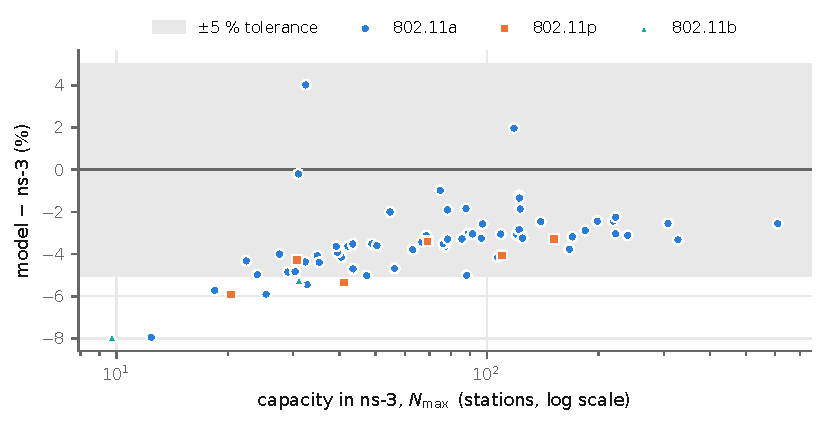
\includegraphics[width=\textwidth]{fig_scorecard}
\caption{The root of \eqref{eq:G5} against \scRows{} capacities stored from ns-3. Below zero, the
model under-predicts the capacity (the safe side).}
\label{fig:scorecard}
\end{figure}

\subsection{The safe side, by traffic source (UJ)}\label{sec:uj}

UJ tested on two new 802.11a cells whether the root of \eqref{eq:G5} stays on the safe side when the
stations' timers jitter or drift, and what frozen phases do (\cref{fig:uj}). It was registered with
two claims for the five non-frozen cells: S, the root at or below ns-3; A, the root and the law
within $\pm5\,\%$. \textbf{S held at all \ujSHeld{}}, the root's error \ujRootMax{} to \ujRootMin\,\%; A held at \ujAHeld, the two misses conservative. With frozen phases (strictly periodic senders,
identical clocks) ns-3's capacity fell by \ujFzDrop\,\% in both cells, to the root
(\ujFzRootMin{} and \ujFzRootMax\,\%) but not past it; the law, which lies slightly above the root,
was optimistic there (\ujFzLawMin{} to \ujFzLawMax\,\%). The registration's outcomes table sent that
case to Mohamed, who decided: \textbf{frozen phases are outside the safe-side claim}. The claim
the report makes is therefore: \emph{the root of \eqref{eq:G5} is on the safe side for timers with
jitter or clock drift} (all new cells, and all stored ones).

\begin{figure}[htbp]
\centering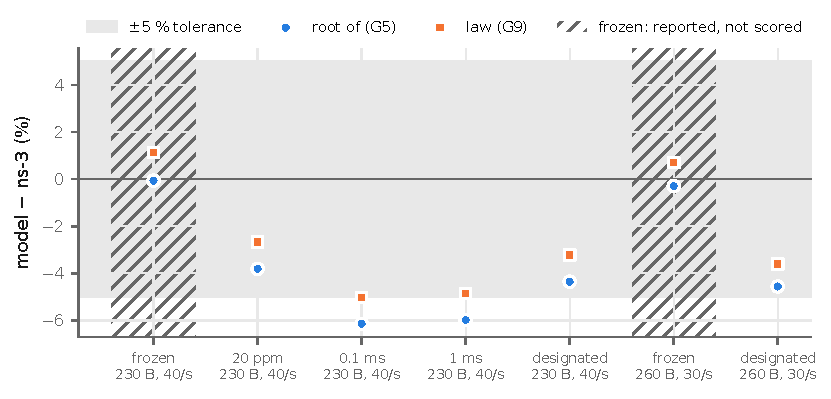
\includegraphics[width=\textwidth]{fig_uj}
\caption{UJ: the error of the root of \eqref{eq:G5} and of the law \eqref{eq:G9} against ns-3, by
traffic source, on two new 802.11a cells. Hatched: frozen phases, reported.}
\label{fig:uj}
\end{figure}

\iffull
\begin{table}[htbp]
\centering\footnotesize
% Generated by analysis/report_numbers.py from results/raw; do not edit by hand.
\begin{tabular}{lllrrllr}
\toprule
Cell & Source & ns-3 $\Nmax$ (95\,\% CI) & Root (\%) & Law (\%) & S & A & Seed $\sigma$ \\
\midrule
JA230F40 & frozen & 32.64 (30.85--33.77) & \textminus{}0.07 & +1.13 & reported & reported & 1.47 \\
JA230F40 & 20 ppm drift & 33.91 (31.64--34.43) & \textminus{}3.81 & \textminus{}2.66 & yes & yes & 1.61 \\
JA230F40 & jitter 0.1 ms & 34.75 (31.81--35.55) & \textminus{}6.14 & \textminus{}5.02 & yes & no & 1.46 \\
JA230F40 & jitter 1 ms & 34.69 (33.72--35.47) & \textminus{}5.98 & \textminus{}4.86 & yes & no & 1.19 \\
JA230F40 & designated & 34.10 (33.91--34.27) & \textminus{}4.36 & \textminus{}3.21 & yes & yes & 0.54 \\
JA260F30 & frozen & 40.09 (39.20--41.28) & \textminus{}0.30 & +0.70 & reported & reported & 1.47 \\
JA260F30 & designated & 41.88 (41.69--42.09) & \textminus{}4.56 & \textminus{}3.61 & yes & yes & 0.46 \\
\bottomrule
\end{tabular}

\caption{UJ in full (S: the root at or below ns-3; A: root and law within $\pm5\,\%$; seed $\sigma$:
the spread of each seed's own crossing).}
\end{table}
\fi

\subsection{The 802.11b arm, and why the sending pattern matters}

At the hardware's own PHY (802.11b, 1\,Mb/s), test UD found the Poisson model low at \udBelow{} of
its \udDOneAll{} small-swarm crossings. At 15--37 stations the root of \eqref{eq:G5} failed the
$\pm5\,\%$ band at \udDRootFailed{} of \udDCells{} cells, all on the safe side (\udDRootMax{} to
\udDRootMin\,\%); at 8--14 stations, with a band widened to $-9\ldots+5\,\%$ at registration, it held
at \udBHeld{} of \udBScored. Term by term, the loss itself was pessimistic by \udThreePMin{} to
\udThreePMax\,\% (D3); a capacity error is far smaller than a loss error because the loss rises
steeply with the load. The cause was the Poisson assumption: ns-3's telemetry source is periodic.
This failure is what \eqref{eq:G25} was written for.

\textbf{UD2 tested \eqref{eq:G25} where UD failed,} on new 802.11b cells at windows 8, 16 and 32 and
loss targets 2, 5 and 10\,\% (\cref{fig:ud2}). It held at all \udQHeld{} of \udQCrossings{}
crossings, with errors from \udQMin{} to \udQMax\,\%, including the \udQPast{} crossings past
occupancy 0.78. The Poisson root beside it erred by \udQPoiMin{} to \udQPoiMax\,\%, outside
$\pm5\,\%$ at \udQPoiOut: UD's failure, repeated on new cells and corrected by \eqref{eq:G25}. UD
itself stays failed as registered.

\begin{figure}[htbp]
\centering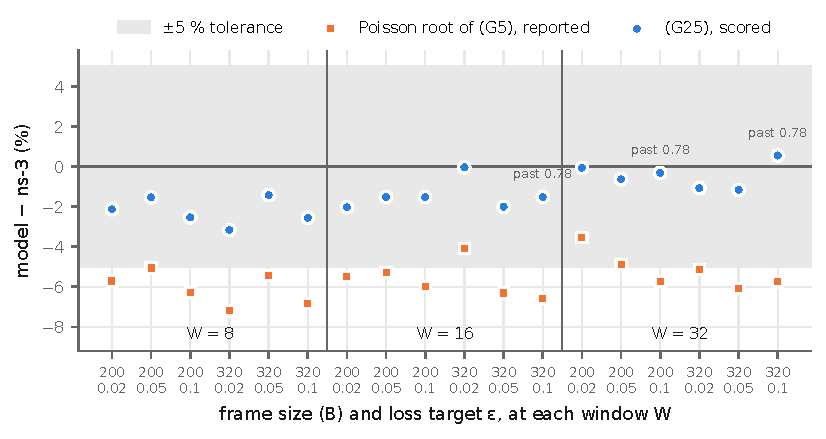
\includegraphics[width=\textwidth]{fig_ud2}
\caption{UD2: \eqref{eq:G25} (scored) and the Poisson root of \eqref{eq:G5} (reported) against
ns-3, 802.11b at 1\,Mb/s, two new frame sizes, three windows and three loss targets.}
\label{fig:ud2}
\end{figure}

\iffull
\begin{table}[htbp]
\centering\footnotesize
% Generated by analysis/report_numbers.py from results/raw; do not edit by hand.
\begin{tabular}{lrllrllr}
\toprule
Cell & $\Wnd$ & $\eps$ & ns-3 $\Nmax$ (95\,\% CI) & \eqref{eq:G25} & Error (\%) & Held & Poisson (\%) \\
\midrule
QB200F10W8 & 8 & 0.02 & 17.30 (17.11--17.44) & 16.93 & \textminus{}2.13 & yes & \textminus{}5.71 \\
QB200F10W8 & 8 & 0.05 & 24.82 (24.62--25.07) & 24.44 & \textminus{}1.54 & yes & \textminus{}5.06 \\
QB200F10W8 & 8 & 0.1 & 32.64 (32.46--32.81) & 31.81 & \textminus{}2.53 & yes & \textminus{}6.29 \\
QB320F8W8 & 8 & 0.02 & 15.47 (15.16--15.73) & 14.98 & \textminus{}3.16 & yes & \textminus{}7.20 \\
QB320F8W8 & 8 & 0.05 & 21.79 (21.60--22.06) & 21.48 & \textminus{}1.42 & yes & \textminus{}5.44 \\
QB320F8W8 & 8 & 0.1 & 28.60 (28.41--28.81) & 27.87 & \textminus{}2.55 & yes & \textminus{}6.82 \\
QB200F10W16 & 16 & 0.02 & 21.62 (21.33--22.08) & 21.18 & \textminus{}2.03 & yes & \textminus{}5.47 \\
QB200F10W16 & 16 & 0.05 & 30.10 (29.85--30.28) & 29.64 & \textminus{}1.51 & yes & \textminus{}5.28 \\
QB200F10W16 & 16 & 0.1 & 37.85 (37.69--38.05) & 37.27 & \textminus{}1.52 & yes & \textminus{}5.97 \\
QB320F8W16 & 16 & 0.02 & 18.82 (18.37--19.31) & 18.82 & \textminus{}0.03 & yes & \textminus{}4.07 \\
QB320F8W16 & 16 & 0.05 & 26.68 (26.50--26.88) & 26.15 & \textminus{}2.00 & yes & \textminus{}6.31 \\
QB320F8W16 & 16 & 0.1 & 33.26 (33.07--33.41) & 32.76 & \textminus{}1.51 (past 0.78) & yes & \textminus{}6.60 \\
QB200F10W32 & 32 & 0.02 & 25.66 (25.44--25.98) & 25.65 & \textminus{}0.06 & yes & \textminus{}3.55 \\
QB200F10W32 & 32 & 0.05 & 34.83 (34.64--35.06) & 34.61 & \textminus{}0.63 & yes & \textminus{}4.88 \\
QB200F10W32 & 32 & 0.1 & 42.16 (42.07--42.23) & 42.03 & \textminus{}0.30 (past 0.78) & yes & \textminus{}5.72 \\
QB320F8W32 & 32 & 0.02 & 23.21 (22.82--23.45) & 22.96 & \textminus{}1.07 & yes & \textminus{}5.13 \\
QB320F8W32 & 32 & 0.05 & 31.07 (30.82--31.26) & 30.71 & \textminus{}1.16 & yes & \textminus{}6.08 \\
QB320F8W32 & 32 & 0.1 & 36.92 (36.81--37.08) & 37.13 & +0.56 (past 0.78) & yes & \textminus{}5.75 \\
\bottomrule
\end{tabular}

\caption{UD2 in full, scored at $\pm5\,\%$.}
\end{table}
\fi

\subsection{The sending pattern}

With Poisson sources the model is \ugPoiMin{} to \ugPoiMax\,\% low on the new cells of UG25.
\eqref{eq:G25} was registered on those \ugCells{} cells and held at all \ugHeld{} (\ugMin{} to
\ugMax\,\%). Past occupancy 0.78 (\uhCells{} further cells at occupancy \uhOccMin--\uhOccMax) it is
optimistic by \uhMin{} to \uhMax\,\%, which is now a stated limit (\cref{fig:g25}).

\begin{figure}[htbp]
\centering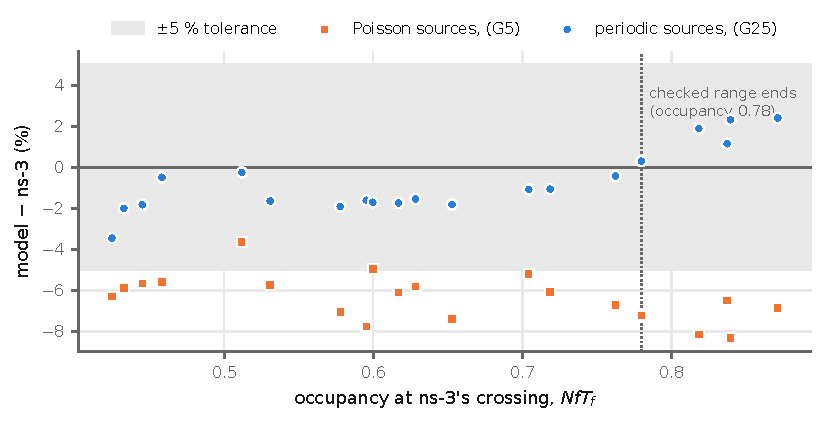
\includegraphics[width=\textwidth]{fig_g25}
\caption{The model's error against ns-3, with Poisson sources, \eqref{eq:G5}, and with periodic
sources, \eqref{eq:G25}, against the occupancy at which ns-3 reaches the loss target.}
\label{fig:g25}
\end{figure}

\subsection{Few stations}

For three to five stations the finite-station form \eqref{eq:FS} held at all \fsHeld{} of \fsCells{}
registered cells, with a tolerance of $\pm15\,\%$ on the loss (\cref{fig:fewstations}). The Poisson
loss \eqref{eq:G5} overstates the loss there by \fsGFiveMin--\fsGFiveMax\,\%.

\begin{figure}[htbp]
\centering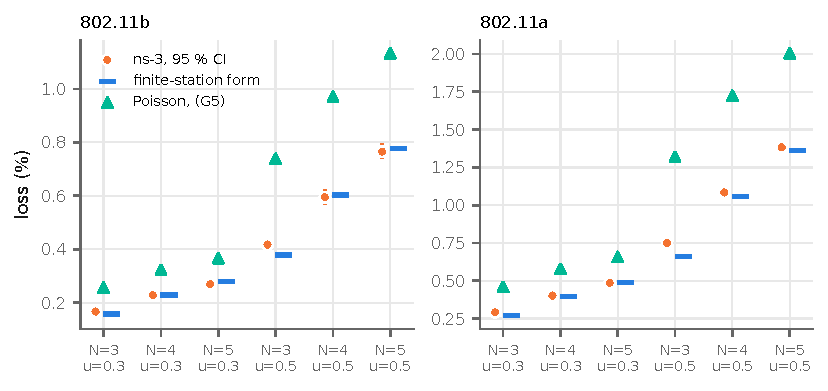
\includegraphics[width=\textwidth]{fig_fewstations}
\caption{UFS: the loss at three to five stations and occupancy 0.3 and 0.5, in ns-3 (30 seeds, 95\,\%
interval), by the finite-station form \eqref{eq:FS} and by the Poisson loss \eqref{eq:G5}.}
\label{fig:fewstations}
\end{figure}

\subsection{Batching}

The gain of batching \eqref{eq:G12} matched ns-3 within \gainMaxAbs\,\% at 802.11a up to 64 records
per frame, and within \gainBMaxAbs\,\% at 802.11b up to 32 (\cref{fig:batching}; reported beside
registered capacity tests UC2 and UD, whose capacities held \ucTwoHeld{} of \ucTwoClaims{} and
\udTwoHeld{} of \udTwoCells).

\begin{figure}[htbp]
\centering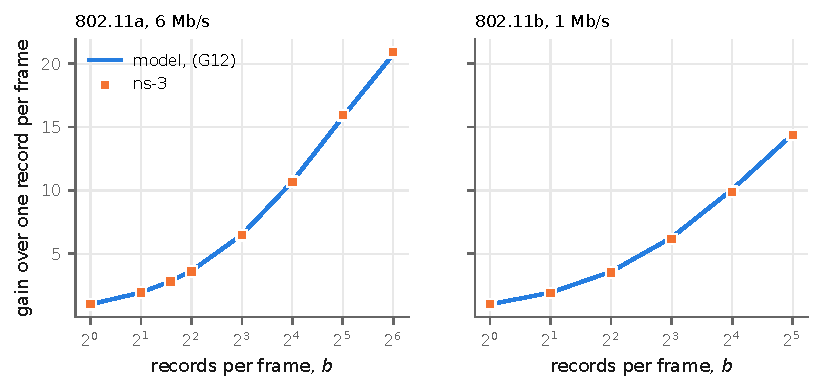
\includegraphics[width=\textwidth]{fig_batching}
\caption{The gain of batching: capacity at $b$ records per frame over capacity at one, less one
station each, \eqref{eq:G12} against ns-3.}
\label{fig:batching}
\end{figure}

\subsection{Capture}

ns-3's capture rule, read from its source and predicted per collision, held at \capHeld{} of
\capTrials{} offsets and power differences (UCAP2). A first capacity test with capture (UF) held
\ufAvgHeld{} of \ufConfigs{} average-delivery claims and only \ufWorstHeld{} of \ufConfigs{}
every-sender claims. Its three causes were found: the half-duplex factor \eqref{eq:G22a} was missing,
the every-sender claim had been scored on a sample minimum rather than on \eqref{eq:G24} or
\eqref{eq:G24a}, and one configuration had a station at the edge of carrier sense. The corrected
test UF2, on new placements and seeds, held all \ufTwoHeld{} of its \ufTwoClaims{} claims, every one
on the safe side: \eqref{eq:G23} within \ufTwoAMin{} to \ufTwoAMax\,\%, the pooled \eqref{eq:G24}
within \ufTwoPoolMin{} to \ufTwoPoolMax\,\%, the window statistic \eqref{eq:G24a} within
\ufTwoWinMin{} to \ufTwoWinMax\,\% (\cref{fig:uf2}).

\begin{figure}[htbp]
\centering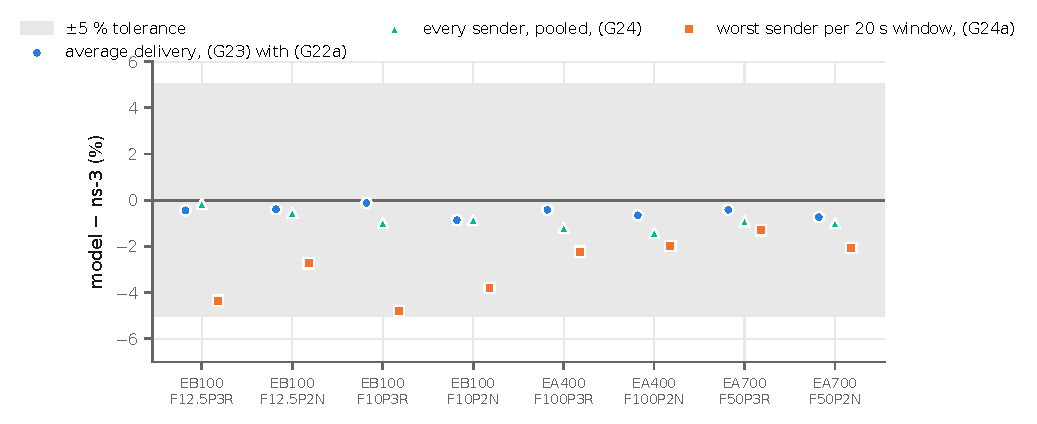
\includegraphics[width=\textwidth]{fig_uf2}
\caption{UF2: the capture laws against ns-3, per configuration (EB: 802.11b, EA: 802.11a; F: frames
per second; P3R: path-loss exponent 3 with Rayleigh fading; P2N: exponent 2, no fading).}
\label{fig:uf2}
\end{figure}

\subsection{Design rules and LoRa}

A key record once in $r=2$ or 4 frames held \ucThreeHeld{} of \ucThreeCells{} (UC3). Fragments spread
over the period held \ucFourSHeld{} of \ucFourSCells{} (UC4S); fragments sent back to back failed
(UC4), and a correction for them removed \burstFixMin--\burstFixMax\,\% of the excess but failed its
own test (UC4B), so the design forbids back-to-back fragments. The best batch under bit errors
\eqref{eq:G19} was predicted as \ucFivePred{} and ns-3's best was \ucFiveBest{} (UC5D1). The LoRa
duty-cycle law held at \lrHeld{} of \lrCells{} cells (UC7).

\subsection{What failed in simulation}

\begin{itemize}
\item \textbf{The split of \eqref{eq:G5} into its three causes} (UC1, D3): the totals hold, the
breakdown does not; ns-3 counts a near-simultaneous start as a detection-window loss.
\item \textbf{Poisson starts at 802.11b} (UD): the capacity \udDRootMax{} to \udDRootMin\,\% low at
15--37 stations; \eqref{eq:G25} then held at all \udQCrossings{} new crossings of UD2.
\item \textbf{The first capture test} (UF): failed for three identified reasons; the corrected test
held on new cells.
\item \textbf{Fragments sent back to back} (UC4, UC4B): outside the model; ruled out by design.
\item \textbf{\eqref{eq:G25} past occupancy 0.78 at 802.11b}: optimistic by \uhMin{} to \uhMax\,\%;
a stated limit.
\item \textbf{Frozen phases} (UJ and the stored cells): ns-3's capacity falls by about
\ujFzDrop\,\%, to the root or past it, and the law is optimistic there (stored: \scLawOptErr\,\%);
excluded from the safe-side claim.
\end{itemize}

% ==================================================================================================
\section{Validation on hardware}\label{sec:hw}
% ==================================================================================================

\textbf{What the hardware tests checked.} W1e, W1j and W1k were registered before the closed form
existed. Their predictions came from the project's event simulation of the DCF access rule
(registered at W1c), which had matched ns-3's capacities at 802.11b within \wOneBErr\,\% (W1b). They test
the access-rule model the closed form is built on, not the closed form's own numbers. W1r's
registration also recorded the closed form's values beside ns-3's; they are compared in
\cref{sec:side}. The first test of the closed form itself on the radios is V1a, below.

\subsection{The closed form on the radios (V1a)}\label{sec:v1a}

On three radios the part of the closed form that applies is the few-station form \eqref{eq:FS}
(three to five stations, occupancy up to 0.5). V1a scored it \emph{as stated}: the standard's window
$\Wnd=32$, rule set A, nothing measured on the radios. The three radios sent at occupancy 0.3, 0.4
and 0.5 in five interleaved rounds, with a control window after each; the session ran remotely and
every validity condition held (background \vaBg\,\%, each radio's link loss alone at most
\vaLinkMax\,\%). The registered tolerance was $\pm15\,\%$ on the loss.

\textbf{The closed form as stated failed at all \vaPoints{} points, on the optimistic side}
(\cref{fig:v1a,tab:v1a}). The radios lost \vaFacMin--\vaFacMax{} times what \eqref{eq:FS} predicts,
and the form lies below the 95\,\% interval of the measurement at every point. ns-3 and the event
simulation, both with the standard rule, sit near the form: the radios lose \vaSimMin--\vaSimMax{}
times what they predict. What misses is therefore the access rule the model assumes, not the
closed form's approximation of that rule. C1 measured the likely cause: the Pi~4s send about half
their frames at DIFS with no backoff, and the Pi~3 waits a fixed \cExtraC\,\us{} longer. A
hardware-matched form, with the radios' measured rule as its input, is the next registered test
(V1b, \cref{sec:next}). The failure was expected and disclosed in the registration; the stored trio
point of W1e and W1r had already pointed to it.

\begin{figure}[htbp]
\centering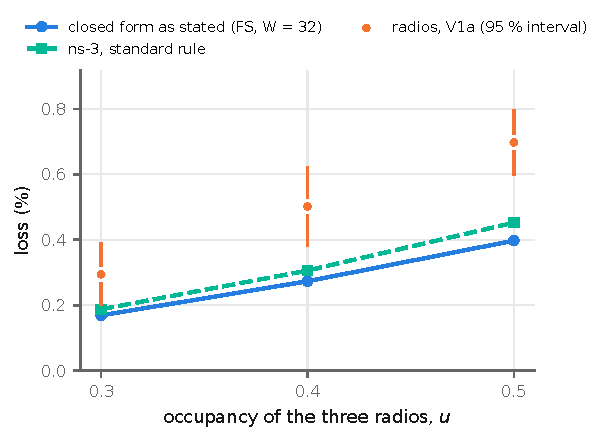
\includegraphics[width=0.66\textwidth]{fig_v1a}
\caption{V1a: the loss of the three radios against the closed form as stated, \eqref{eq:FS} at
$\Wnd=32$, and ns-3 with the standard rule.}
\label{fig:v1a}
\end{figure}

\begin{table}[htbp]
\centering\small
% Generated by analysis/report_numbers.py from results/raw; do not edit by hand.
\begin{tabular}{rrlrrlrrr}
\toprule
$\occ$ & $f$ & Radios, \% (95\,\% CI) & \eqref{eq:FS}, \% & Error (\%) & Held & ns-3, \% & Event sim., \% & \eqref{eq:G5}, \% \\
\midrule
0.3 & 52 & 0.294 (0.198--0.391) & \textbf{0.169} & \textminus{}42.7 & \textbf{no} & 0.188 & 0.193 & 0.263 \\
0.4 & 70 & 0.501 (0.378--0.625) & \textbf{0.273} & \textminus{}45.5 & \textbf{no} & 0.306 & 0.312 & 0.468 \\
0.5 & 87 & 0.697 (0.597--0.798) & \textbf{0.397} & \textminus{}43.0 & \textbf{no} & 0.452 & 0.446 & 0.743 \\
\bottomrule
\end{tabular}

\caption{V1a, scored at $\pm15\,\%$. The last three columns were reported, not scored;
\eqref{eq:G5} lies outside its stated range at three stations. Its closeness to the radios
(\vaGfiveMin{} to \vaGfiveMax\,\%) is not evidence for it: periodic sources make it pessimistic for
three stations, while the radios' rule adds collisions, so two departures act in opposite
directions; the matched form will separate them.}
\label{tab:v1a}
\end{table}

\subsection{Contention}

\Cref{fig:hw} shows the loss of two and three radios at occupancy 0.50, 0.70 and 0.85. In W1e (frame
burst on) \weHeld{} of \wePoints{} points lay inside the bands registered from the event
simulation; the miss was pi-A with pi-B at the lowest load, \weMissRatio{} times the prediction against a band
top of \weMissTop. In W1r (frame burst off) the hardware lies between two ns-3 settings of slot and
DIFS: inside the 95\,\% interval at \wrInTwenty{} of \wrPoints{} points for slot 20\,\us/DIFS
50\,\us, and \wrInNine{} for slot 9\,\us/DIFS 28\,\us. The pairs with the Pi 3 lose more than ns-3
predicts; ns-3 had been given windows inferred from each radio's sending rate, $\Wnd=\wrWinPi$ for
the Pi 4s and \wrWinPiThree{} for the Pi 3, and C1 later showed both to be wrong in kind
(\cref{sec:window}).

\begin{figure}[htbp]
\centering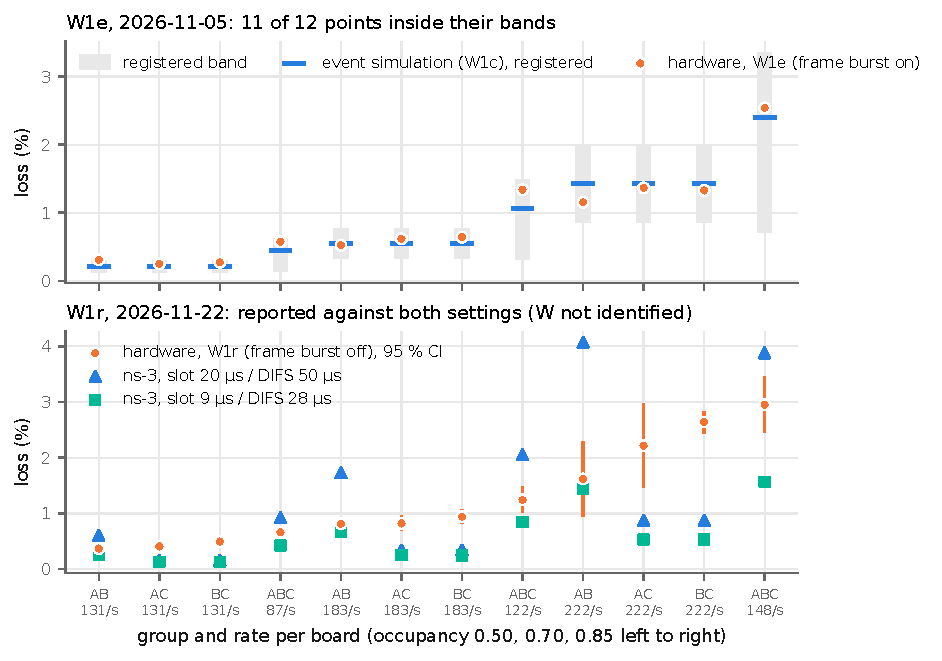
\includegraphics[width=\textwidth]{fig_hw_contention}
\caption{Hardware contention. Top: W1e against its registered prediction (the event simulation of
W1c). Bottom: W1r against ns-3 with two settings of slot and DIFS (the contention window was not
known; \cref{sec:window}).}
\label{fig:hw}
\end{figure}

\subsection{The capacity ratio}

On four radios (pi-A, pi-B, the Pi 3 and the TP-Link), the capacity of the design (one signature per
frame of four records) divided by that of per-record signing was \ratioJ{} in W1j and \ratioK{} in
W1k, against the registered \ratioModel{} (band \ratioLo--\ratioHi; \cref{fig:ratio}). The capacities
themselves were \crossAuthJ{} and \crossPerJ{} capacity-equivalent stations in W1j, against
\crossAuthModel{} and \crossPerModel{} (\crossAuthErr{} and \crossPerErr\,\%), attributed in W1j
to capture at the receivers, while the ratio moved by \ratioErr\,\%.

\begin{figure}[htbp]
\centering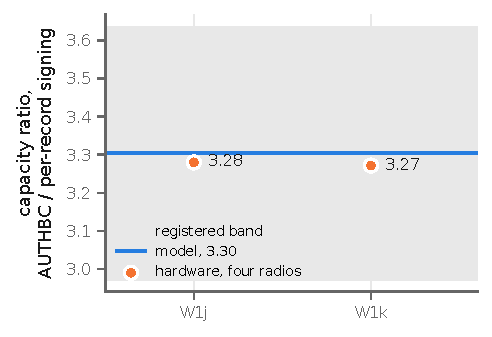
\includegraphics[width=0.5\textwidth]{fig_ratio}
\caption{The capacity ratio on four radios against the registered value.}
\label{fig:ratio}
\end{figure}

\subsection{Loss on air}

W3a traced every frame on air at 802.11b and replayed the traces through the project's real
decoder. All \wtHeld{} of \wtClaims{} registered claims held: real loss hurts the frames that depend
on a key record no more than independent loss would; the design loses only its own frames; and the
loss grows with frame length less steeply than a bit-error model predicts.

\subsection{Capture}

In W1q (the Pi 3 receiving, pi-A's power stepped) \wqHeld{} of \wqScored{} registered predictions
held. The one that failed is the finding: at a measured difference of only \wqThreeDelta\,dB the Pi
3 kept the stronger frame in \wqThreeQ{} of collisions, where ns-3's rule keeps none below 4\,dB.
Capture on this radio is gradual, not a step. Three of W1q's five power steps were void because the
received signal fell by less than the set power (\cref{sec:window}). W1s then tested the gradual
curve on new power steps: \wsCurveHeld{} of \wsCurveScored{} held, so the curve is not used; the
boards' radio geometry had changed between the sessions (\cref{fig:capture}).

\begin{figure}[htbp]
\centering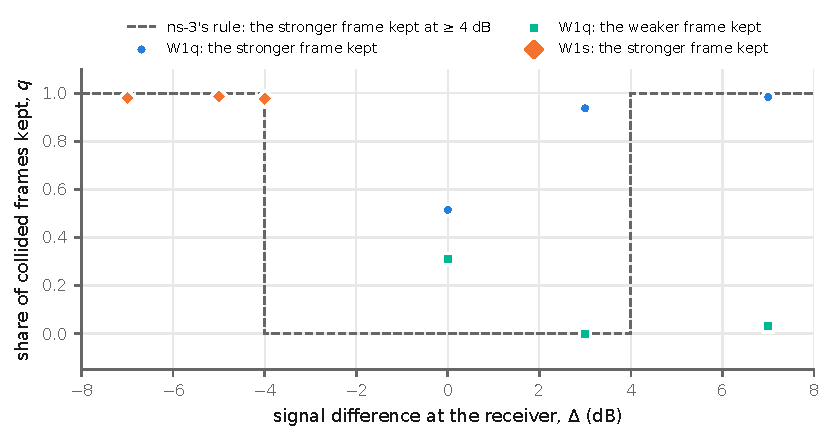
\includegraphics[width=\textwidth]{fig_capture_hw}
\caption{The share of collided frames the receiver kept, against the signal difference. Dashed:
ns-3's 4\,dB rule. W1q's points are from its valid steps; W1s's from its new steps.}
\label{fig:capture}
\end{figure}

\subsection{The contention window, and the radios' own timing}\label{sec:window}

The model needs each radio's contention window $\Wnd$, slot and DIFS; radios do not report them.
\textbf{W1p} tested two settings derived from each radio's sending rate: a saturated pair lost
\wpLoss{} at \wpFps{} frames/s, against ns-3's \wpTwentyLoss{} and \wpNineLoss: neither fits.
\textbf{W1s} re-derived both settings once and tested them at a new frame length: the pair lost
\wsPairLoss{} at \wsPairFps{} frames/s, against \wsTwentyLoss{} and \wsNineLoss: neither fits again,
so the window is recorded as not identifiable without a frame sniffer.

A sniffer was therefore added (the TP-Link in monitor mode, with a one-line driver change that
exports the chip's per-frame hardware timestamp). Its gate S0 \textbf{failed}: it recorded \sgA,
\sgB{} and \sgC{} of the three radios' frames, against the 0.99 required, though the radios
themselves received almost all of them; the misses follow neither the board nor its place, and a
probe at another placement (P1) did not reach 0.99 either; its planned placements 3\,m and 5\,m
away have not run. The same gate showed that the received signal
falls by \sgFalls\,dB when pi-A's set power falls by 3, 6 and 9\,dB; the Pi 3 registered a similar
compression, so the transmitter is the more likely cause, but this is not established. The sniffer
is used for timing only, under a stated rule, until a better adapter arrives.

\textbf{C1 (calibration, not validation)} measured each radio alone with the sniffer's microsecond
timestamps (\cref{fig:c1}). For both Pi 4s the gap after a frame has a floor of \cFloorA\,\us{} (the
standard's DIFS) and a 20\,\us{} lattice (the standard's slot); \cShareMinA--\cShareMaxB{} of their
frames are sent at DIFS with no backoff, and the rest spread over \cWminA{} slots. Under the
standard's rule a saturated sender draws its backoff from $0\ldots\Wnd-1$ after every frame, so only
about $1/\Wnd$ of frames (3\,\% at $\Wnd=32$) would go out at DIFS. Departures of commercial 802.11b cards from the standard's backoff have been
measured before \cite{bianchi2007cards}. The share did not change with a
back-to-back sender (\cShareKA), so it is the radio's own behaviour, not the sending pattern. The
Pi 3's floor is \cFloorC\,\us{} (\cExtraC\,\us{} more than DIFS) and \cShareMinC--\cShareMaxC{} of its
frames skip the backoff, close to the standard's $1/\Wnd$, with \cWminC--\cWmaxC{} slots. Across
frame sizes the airtime grows by \cSlope\,\us{} per byte (1\,Mb/s), with an intercept of
\cInterA\,\us{} (the long preamble, 192\,\us, plus DIFS). These are inputs for a hardware-matched
model; nothing has yet been validated with them.

\begin{figure}[htbp]
\centering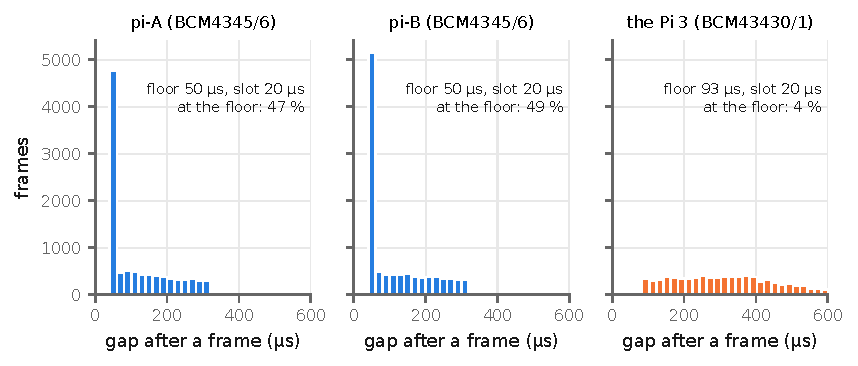
\includegraphics[width=\textwidth]{fig_c1_gaps}
\caption{C1: the gap after each frame, for each radio sending alone (145\,B frames). One bin per
backoff slot.}
\label{fig:c1}
\end{figure}

\iffull
\begin{figure}[htbp]
\centering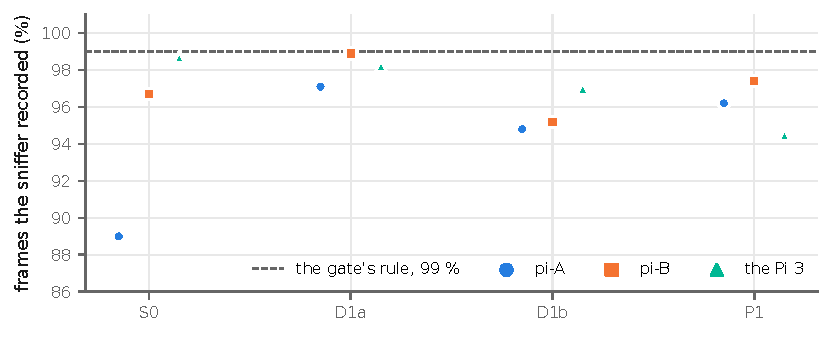
\includegraphics[width=\textwidth]{fig_sniffer}
\caption{The share of each radio's frames the sniffer recorded, session by session (S0: the gate;
D1a, D1b: diagnostics, pi-A and pi-B swapped in D1b; P1: the probe). The misses follow neither the
board nor its place.}
\label{fig:sniffer}
\end{figure}
\fi

\subsection{What failed on hardware}

\begin{itemize}
\item \textbf{The closed form as stated} (V1a): \eqref{eq:FS} at $\Wnd=32$ lies \vaErrB{} to
\vaErrA\,\% from the radios' loss at occupancy 0.3--0.5; the standard access rule is what differs.
\item \textbf{The window, from sending rates} (W1p, W1s): neither setting of slot and DIFS fits; the
window was not identifiable that way. C1 shows why: the Pi 4s skip the backoff for about half their
frames, which no single window describes.
\item \textbf{ns-3's 4\,dB capture step} (W1q): the radio captures at 1.5\,dB; the gradual curve
then failed its own check on new steps (W1s) after the geometry changed.
\item \textbf{The sniffer's gate} (S0, P1): the adapter misses \snifMissMin--\snifMissMax\,\% of frames, drifting between
sessions.
\item \textbf{Power steps}: the received signal falls by less than the set power, most likely at the
transmitter.
\end{itemize}

% ==================================================================================================
\section{Model, simulation and hardware side by side}\label{sec:side}
% ==================================================================================================

\Cref{tab:threeway} puts every source of a prediction beside the two hardware sessions, for the same
radios and rates: the closed forms (as recorded in W1r's registration, at the standard's
$\Wnd=32$), W1c's event simulation (W1e's registered prediction), ns-3 with two settings of slot and
DIFS, and the hardware with frame burst on (W1e) and off (W1r).

\begin{table}[htbp]
\centering\footnotesize
% Generated by analysis/report_numbers.py from results/raw; do not edit by hand.
\begin{tabular}{lrrrrrrrrrr}
\toprule
Radios & $\occ$ & $f$ & \eqref{eq:G5} & \eqref{eq:G25} & Finite & Event model & ns-3, $\slot=20$ & ns-3, $\slot=9$ & W1e & W1r \\
\midrule
AB & 0.50 & 131 & 0.41 & 0.30 & -- & 0.22 & 0.60 & 0.25 & 0.31 & 0.37 \\
AC & 0.50 & 131 & 0.41 & 0.30 & -- & 0.22 & 0.16 & 0.13 & 0.25 & 0.41 \\
BC & 0.50 & 131 & 0.41 & 0.30 & -- & 0.22 & 0.16 & 0.13 & 0.27 & 0.50 \\
ABC & 0.50 & 87 & 0.74 & 0.55 & 0.40 & 0.45 & 0.92 & 0.42 & 0.58 & 0.66 \\
AB & 0.70 & 183 & 0.83 & 0.54 & -- & 0.55 & 1.73 & 0.67 & 0.52 & 0.81 \\
AC & 0.70 & 183 & 0.83 & 0.54 & -- & 0.55 & 0.34 & 0.25 & 0.62 & 0.82 \\
BC & 0.70 & 183 & 0.83 & 0.54 & -- & 0.55 & 0.34 & 0.24 & 0.64 & 0.94 \\
ABC & 0.70 & 122 & 1.66 & 1.10 & -- & 1.06 & 2.05 & 0.84 & 1.34 & 1.24 \\
AB & 0.85 & 222 & 1.31 & 0.79 & -- & 1.43 & 4.07 & 1.44 & 1.15 & 1.62 \\
AC & 0.85 & 222 & 1.31 & 0.79 & -- & 1.43 & 0.87 & 0.53 & 1.37 & 2.21 \\
BC & 0.85 & 222 & 1.31 & 0.79 & -- & 1.43 & 0.87 & 0.53 & 1.33 & 2.64 \\
ABC & 0.85 & 148 & 2.82 & 1.69 & -- & 2.40 & 3.88 & 1.57 & 2.54 & 2.95 \\
\bottomrule
\end{tabular}

\caption{Loss (\%) of two and three radios, 802.11b at 1\,Mb/s, $f$ frames per second per radio.
For the pairs, \eqref{eq:G5} and \eqref{eq:G25} lie outside their stated range (two stations;
\eqref{eq:G25} needs 8 or more others); the finite-station form is shown only where it was accepted
(three stations, occupancy 0.5). The ns-3 values for the pairs with the Pi 3 use its inferred window
of \wrWinPiThree{} slots.}
\label{tab:threeway}
\end{table}

\textbf{What the comparison shows.}
\begin{itemize}
\item \textbf{The trio at occupancy 0.5}, the one point inside every model's range: \eqref{eq:FS},
the event simulation, ns-3 at slot 9\,\us{} and both hardware sessions lie between \twTrioLo{} and
\twTrioHi\,\%; \eqref{eq:G5} and ns-3 at slot 20\,\us{} lie above them.
\item \textbf{The pairs:} no closed form is claimed for two stations. ns-3's values for the pairs
with the Pi 3 are \twPiThreeLo--\twPiThreeHi{} times below the hardware, because ns-3 was given a window of
\wrWinPiThree{} slots for the Pi 3; C1 measured \cWminC--\cWmaxC{} plus a fixed \cExtraC\,\us.
\item \textbf{The same radios, two sessions} (W1e and W1r) differ by up to a factor of \twSessMax{} for the
pairs with the Pi 3: frame burst, placement and day all changed between them. A hardware number is a
property of a session, not only of the radios.
\end{itemize}

\begin{table}[htbp]
\centering\small
\begin{tabularx}{\textwidth}{>{\raggedright\arraybackslash}p{3.9cm}>{\raggedright\arraybackslash}p{2.4cm}>{\raggedright\arraybackslash}p{2.4cm}L}
\toprule
Quantity & Model & ns-3 & Hardware \\
\midrule
loss of three radios at $\occ=0.5$ (V1a) & \vaFinC\,\% \eqref{eq:FS} & \vaNsC\,\% (standard rule) & \vaLossC\,\% \\
capacity ratio, design over per-record signing (4 radios) & \ratioModel{} (event simulation) & -- & \ratioJ, \ratioK{} (W1j, W1k) \\
gain of batching, 802.11a, $b$ up to 64 & \eqref{eq:G12} & within \gainMaxAbs\,\% & not tested (V2) \\
capture at a signal difference of \wqThreeDelta\,dB & \eqref{eq:G22} with the input $q$ & $q=0$ (4\,dB rule) & $q=\wqThreeQ$ (W1q) \\
slot, DIFS & 20\,\us, 50\,\us{} (standard) & the same & 20\,\us, \cFloorA\,\us{} (Pi 4s); 20\,\us, \cFloorC\,\us{} floor (Pi 3) \\
frames sent at DIFS with no backoff, saturated & about $1/\Wnd$ (the standard's backoff after every frame) & not measured & \cShareMinA--\cShareMaxB{} (Pi 4s); \cShareMinC--\cShareMaxC{} (Pi 3) \\
airtime per byte at 1\,Mb/s & 8\,\us & 8\,\us & \cSlope\,\us{} (C1) \\
\bottomrule
\end{tabularx}
\caption{One quantity at a time: what the model assumes or predicts, what ns-3 does, what the radios
do.}
\label{tab:side}
\end{table}

% ==================================================================================================
\section{What remains to be tested}\label{sec:next}
% ==================================================================================================

\Cref{tab:coverage} maps each part of the model against where it has been tested.
\Cref{tab:next} lists the open tests, in the order they can run.

\begin{table}[htbp]
\centering\small
\begin{tabularx}{\textwidth}{>{\raggedright\arraybackslash}p{4.2cm}LL}
\toprule
Part of the model & ns-3 & Hardware \\
\midrule
accounting and batching, \eqref{eq:G1}--\eqref{eq:G3}, \eqref{eq:G10}--\eqref{eq:G13} & held (UC2, UD) & ratio held (W1j, W1k, event simulation); gain on air not tested (V2) \\
loss \eqref{eq:G4}--\eqref{eq:G5} & total held; split into causes failed (UC1) & as stated, \textbf{failed} (V1a, through \eqref{eq:FS}); the radios' access rule differs (C1) \\
two-constant law \eqref{eq:G6}--\eqref{eq:G9} & held where valid, \scLawIn{} of \scLawRows & not tested \\
design rules \eqref{eq:G16}--\eqref{eq:G21} & held (UC3, UC4S, UC5D1, UC7); back-to-back fragments failed & not tested \\
capture \eqref{eq:G22}--\eqref{eq:G24a} & held after correction (UCAP2, UF2) & the input $q$ measured, partly (W1q); in contention not tested (V3, V4) \\
sending pattern \eqref{eq:G25}, \eqref{eq:FS} & held to occupancy 0.78, and at 802.11b at every window and target (UD2); 3--5 stations held & \eqref{eq:FS} as stated \textbf{failed} (V1a); with the measured rule: V1b \\
hidden stations; two stations & not tested; no closed form & not tested \\
\bottomrule
\end{tabularx}
\caption{The coverage map: where each part of the model has been tested, and how it came out.}
\label{tab:coverage}
\end{table}

\begin{table}[htbp]
\centering\small
\begin{tabularx}{\textwidth}{>{\raggedright\arraybackslash}p{3.6cm}>{\raggedright\arraybackslash}p{1.9cm}L>{\raggedright\arraybackslash}p{2.9cm}}
\toprule
Test & Where & What it would show & Waits on \\
\midrule
S0b: the AR9271 sniffer's gate, beside the TP-Link & hardware & whether a second sniffer records $\ge99\,\%$ of frames; whether the power steps compress at the sender & the adapter (by 30 November 2026) \\
C1 in W1q's layout (L1); P1 at 3\,m and 5\,m & hardware & the timing of C1 where the capture sessions ran; whether distance lets the TP-Link reach 0.99 & Mohamed at the boards \\
C2: saturated pairs with the sniffer & hardware & the access rule two radios use under contention: who skips the backoff, and when & S0b \\
C3: the capture curve, both signs of the signal difference & hardware & $q$ against the signal difference for the real receiver & S0b \\
The parameter file & -- & the measured slot, DIFS, access rule, airtime and link losses, as one input set & C1--C3; Mohamed's review \\
The hardware-matched form: \eqref{eq:FS} with each radio's measured backoff and fixed delay, checked against the event simulation & model & the closed form with the radios' own rule, derived and checked before any test & Mohamed's acceptance of the derivation \\
V1b: the matched form on a new session of the three radios, as V1a & hardware & whether the closed form predicts the radios once it is given their rule & C2; the parameter file \\
V2: batching on air & hardware & the gain \eqref{eq:G12} on real radios & the parameter file \\
V3, V4: capture in contention; every-sender statistics & hardware & \eqref{eq:G22}--\eqref{eq:G24a} on real radios & C3 \\
Transmitter or receiver: does pi-A's output follow its set power? & hardware & where the power steps compress & an external receiver (HackRF) if S0b cannot separate them \\
Hidden stations & ns-3 & the term $2h\nu\Tf$ & outside the current scope \\
Two stations; fragments sent back to back & model & a closed form (none exists) & a derivation \\
\bottomrule
\end{tabularx}
\caption{The open tests. Calibration (C) sets the inputs; validation (V) tests predictions made from
them; no session does both.}
\label{tab:next}
\end{table}

If no suitable adapter is available by 30 November 2026, C2 and C3 use the receivers' logs, as W1p
and W1q did, with the sniffer for timing only, and the report of those sessions states the
limitation.

% ==================================================================================================
\section{Conclusions}
% ==================================================================================================

\begin{itemize}
\item \textbf{What can be claimed now.} The closed form predicts ns-3's capacity within $\pm5\,\%$ in
\scRootIn{} of \scRows{} stored cases, and its root lies on the safe side for every timer with jitter
or clock drift (UJ); frozen phases are excluded. Its extensions
for the sending pattern and for capture hold in registered ns-3 tests on new cells. On hardware, the
capacity ratio of the design over per-record signing matches the registered value (\ratioJ{}
against \ratioModel), and the access-rule model behind the closed form fell inside the registered
bands at \weHeld{} of \wePoints{} contention points.
\item \textbf{What cannot be claimed yet.} That the closed form predicts the radios' loss: as stated,
with the standard's access rule, it does not (V1a: the radios lose \vaFacMin--\vaFacMax{} times its
prediction, and ns-3 with the same rule misses alike); whether it does with the radios' measured
rule is the next test (V1b). That the model's access rule is the radios': the Pi 4s send about
half their frames with no backoff, which the standard's rule does not include. That ns-3's 4\,dB
capture step describes the real receiver: it captures gradually.
\item \textbf{Next.} The hardware-matched form (derived, then checked against the event simulation);
a sniffer that passes its gate and the calibration sessions C2 and C3; the parameter file for
review; then V1b and the validation sessions V2--V4 against the matched model and ns-3.
\end{itemize}

\iffull
\appendix
% ==================================================================================================
\section{Notation}
% ==================================================================================================
\begin{table}[htbp]
\centering\small
\begin{tabular}{ll}
\toprule
Symbol & Meaning \\
\midrule
$\Lam$ & records per second per station \\
$b$, $\bstar$, $\bM$ & batch (records per frame); the batch used; the largest that fits \\
$\Dmax$, $\Dnet$, $\Sq$ & deadline; deadline net of the delay $\Sq$ \\
$\Phi$, $\Psi$, $\Bud$ & cost per frame, cost per record, budget of a resource \\
$\Tf$ & a frame's airtime \\
$f$, $\nu$ & frames per second per station; start rate of the other stations, $(N-1)f$ \\
$\occ$ & occupancy, $N f\Tf$ \\
$\slot$, $\Difs$, $\Wnd$, $\delta$ & slot, DIFS, contention window, preamble-detection time \\
$\eps$, $\eps'$, $\epsw$ & loss target; with capture, average; with capture, every sender \\
$\rhostar$, $\tauzero$, $\tauhat$, $\kappa$ & the two constants of \eqref{eq:G9}; per-frame channel cost; $1-\eps/2$ \\
$\Kbar$, $a$, $\gamma$, $\eta$ & co-waiting frames; busy, gap and immediate-access loads \\
$\pcoll$, $q$, $\qeff$, $\ell$, $\ellbar$ & collision loss; capture probability; with the half-duplex factor; link loss; its average \\
$\Ninf$, $\beta$, $\Gain$ & capacity limit, half-gain batch, gain of batching \\
$\Rper$ & periodic-source ratio of \eqref{eq:G25} \\
$m$, $M$, $\pi$ & bystanders, co-waiting count and co-waiting probability of \eqref{eq:FS} \\
$z_N$ & expected maximum of $N$ standard normal draws \\
\bottomrule
\end{tabular}
\end{table}

% ==================================================================================================
\section{Failed attempts and corrections, kept visible}
% ==================================================================================================

\begin{itemize}
\item \textbf{UF (capture, first test).} \ufAvgHeld{} of \ufConfigs{} and \ufWorstHeld{} of
\ufConfigs{} held. Three causes, each found from logged state, not assumed: the half-duplex factor
\eqref{eq:G22a} had been omitted from both the law and its check script, so their agreement could not
reveal it; the every-sender claim had been scored on a sample minimum, an extreme that grows with
the number of senders, rather than on \eqref{eq:G24} or \eqref{eq:G24a}; one configuration placed a
station at the edge of carrier sense, outside one collision domain. UF stays failed; UF2 tested the
corrections on new placements and seeds.
\item \textbf{UC4B (a burst correction for back-to-back fragments).} Removed
\burstFixMin--\burstFixMax\,\% of the excess but failed on both scored cells, on the optimistic
side. Not used; the design rule forbids the case.
\item \textbf{UG25H: \eqref{eq:G25} at high occupancy.} An earlier estimate from capture runs put
the error at \fOneFortyMin--\fOneFortyMax\,\%; measured once without capture it is \uhMin{} to \uhMax\,\%. The band of
the earlier estimate held at none of the four cells.
\item \textbf{W1p and W1s (the window from sending rates).} Two re-derivations, two failures; by
Mohamed's rule no third attempt was made, and the window was recorded as not identifiable without a
sniffer.
\item \textbf{W1q's gradual capture curve.} Fitted after W1q's failure, then checked on new steps in
W1s: \wsCurveHeld{} of \wsCurveScored{}; not used.
\item \textbf{S0's timing criterion.} The registration compared the median of the sniffer's
start-to-start intervals with the receivers' mean cycle; with half the gaps at DIFS the median was
bound to fall below the mean. The means agree within \sZeroMeanMin--\sZeroMeanMax\,\%. A corrected gate (S0b) compares
mean with mean on new windows.
\item \textbf{C1's estimators.} Two estimators were revised after the gate's rate checks and before
C1 ran (the lattice had picked a harmonic; $\Wnd-1$ from a percentile read the long tail); both were
tested on synthetic gaps of known slot and window first, and the revision is disclosed in C1's
registration.
\end{itemize}

\FloatBarrier
% ==================================================================================================
\section{Every test, in full}
% ==================================================================================================

Each table is generated from the test's scored file in \texttt{results/raw/}.

\subsection{Simulation}

{\footnotesize\setlength{\tabcolsep}{3pt}
\renewcommand{\longcap}{Every stored ns-3 capacity against the law \eqref{eq:G9} and the root of
\eqref{eq:G5} (errors in \%; negative is the safe side; ``--'': the law is not valid for that
frame).\label{tab:scorecard}}
% Generated by analysis/report_numbers.py from results/raw; do not edit by hand.
\begin{longtable}{>{\raggedright}p{2.7cm}lclllr>{\raggedright}p{2.2cm}rrr}
\caption{\longcap}\\
\toprule
Source & Cell & Std & $\Wnd$ & $\eps$ & $f$ & $\Tf$ (\textmu s) & Jitter & ns-3 $\Nmax$ & Law (\%) & Root (\%) \\
\midrule\endfirsthead
\toprule
Source & Cell & Std & $\Wnd$ & $\eps$ & $f$ & $\Tf$ (\textmu s) & Jitter & ns-3 $\Nmax$ & Law (\%) & Root (\%) \\
\midrule\endhead
\bottomrule\endfoot
ns3\_\allowbreak{}nmax\_\allowbreak{}direct & A & a & 16 & 0.05 & 50 & 304 & 0/0ppm & 30.97 & +1.6 & \textminus{}0.2 \\
ns3\_\allowbreak{}nmax\_\allowbreak{}direct & A & a & 16 & 0.05 & 50 & 304 & 0.1/5000ppm & 32.69 & \textminus{}3.8 & \textminus{}5.5 \\
ns3\_\allowbreak{}nmax\_\allowbreak{}direct & A & a & 16 & 0.05 & 50 & 304 & 20/0ppm & 32.32 & \textminus{}2.6 & \textminus{}4.4 \\
ns3\_\allowbreak{}nmax\_\allowbreak{}direct & B & a & 16 & 0.05 & 12.5 & 472 & 0/0ppm & 87.76 & \textminus{}1.0 & \textminus{}1.8 \\
ns3\_\allowbreak{}nmax\_\allowbreak{}direct & B & a & 16 & 0.05 & 12.5 & 472 & 80/0ppm & 88.85 & \textminus{}2.2 & \textminus{}3.0 \\
ns3\_\allowbreak{}nmax\_\allowbreak{}direct & C & a & 16 & 0.05 & 50 & 268 & 0/0ppm & 32.41 & +6.4 & +4.0 \\
ns3\_\allowbreak{}nmax\_\allowbreak{}direct & C & a & 16 & 0.05 & 50 & 268 & 20/0ppm & 35.26 & \textminus{}2.2 & \textminus{}4.4 \\
ns3\_\allowbreak{}nmax\_\allowbreak{}direct & D & a & 16 & 0.05 & 12.5 & 304 & 0/0ppm & 118.3 & +3.9 & +2.0 \\
ns3\_\allowbreak{}nmax\_\allowbreak{}direct & D & a & 16 & 0.05 & 12.5 & 304 & 0.1/0ppm & 122.13 & +0.6 & \textminus{}1.2 \\
ns3\_\allowbreak{}nmax\_\allowbreak{}direct & D & a & 16 & 0.05 & 12.5 & 304 & 0.1/5000ppm & 122.92 & \textminus{}0.1 & \textminus{}1.9 \\
ns3\_\allowbreak{}nmax\_\allowbreak{}direct & D & a & 16 & 0.05 & 12.5 & 304 & 1/0ppm & 122.27 & +0.5 & \textminus{}1.3 \\
ns3\_\allowbreak{}nmax\_\allowbreak{}direct & D & a & 16 & 0.05 & 12.5 & 304 & 80/0ppm & 124.55 & \textminus{}1.4 & \textminus{}3.1 \\
ns3\_\allowbreak{}nmax\_\allowbreak{}direct & E & a & 16 & 0.05 & 12.5 & 828 & 0/0ppm & 54.74 & \textminus{}1.7 & \textminus{}2.0 \\
ns3\_\allowbreak{}nmax\_\allowbreak{}direct & E & a & 16 & 0.05 & 12.5 & 828 & 80/0ppm & 56.28 & \textminus{}4.4 & \textminus{}4.7 \\
ns3\_\allowbreak{}nmax\_\allowbreak{}direct & F & a & 16 & 0.05 & 12.5 & 568 & 0/0ppm & 74.75 & \textminus{}0.4 & \textminus{}1.0 \\
ns3\_\allowbreak{}nmax\_\allowbreak{}direct & F & a & 16 & 0.05 & 12.5 & 568 & 80/0ppm & 76.83 & \textminus{}3.1 & \textminus{}3.6 \\
ns3\_\allowbreak{}nmax\_\allowbreak{}direct & G & a & 16 & 0.05 & 12.5 & 572 & 80/0ppm & 76.26 & \textminus{}3.0 & \textminus{}3.5 \\
ns3\_\allowbreak{}nmax\_\allowbreak{}direct & H & a & 16 & 0.05 & 12.5 & 364 & 80/0ppm & 108.91 & \textminus{}1.8 & \textminus{}3.0 \\
ns3\_\allowbreak{}nmax\_\allowbreak{}direct & I & a & 16 & 0.05 & 12.5 & 456 & 80/0ppm & 91.34 & \textminus{}2.2 & \textminus{}3.0 \\
ns3\_\allowbreak{}nmax\_\allowbreak{}direct & RA & a & 16 & 0.05 & 20 & 304 & 50/0ppm & 78.35 & \textminus{}1.5 & \textminus{}3.3 \\
ns3\_\allowbreak{}nmax\_\allowbreak{}direct & RB & a & 16 & 0.05 & 5 & 472 & 200/0ppm & 219.19 & \textminus{}1.6 & \textminus{}2.4 \\
ns3\_\allowbreak{}nmax\_\allowbreak{}direct & RC & a & 16 & 0.05 & 20 & 268 & 50/0ppm & 85.58 & \textminus{}1.1 & \textminus{}3.3 \\
ns3\_\allowbreak{}nmax\_\allowbreak{}direct & RD & a & 16 & 0.05 & 5 & 304 & 200/0ppm & 307.95 & \textminus{}0.8 & \textminus{}2.5 \\
ns3\_\allowbreak{}nmax\_\allowbreak{}direct & SM & a & 16 & 0.05 & 50 & 200 & 20/0ppm & 42.15 & \textminus{}0.0 & \textminus{}3.6 \\
ns3\_\allowbreak{}nmax\_\allowbreak{}direct & ST & a & 16 & 0.05 & 50 & 216 & 20/0ppm & 40.44 & \textminus{}1.0 & \textminus{}4.1 \\
ns3\_\allowbreak{}nmax\_\allowbreak{}direct & SG & a & 16 & 0.05 & 50 & 224 & 20/0ppm & 39.44 & \textminus{}0.9 & \textminus{}3.9 \\
ns3\_\allowbreak{}nmax\_\allowbreak{}direct & SE & a & 16 & 0.05 & 50.5 & 268 & 19.802/0ppm & 34.81 & \textminus{}1.9 & \textminus{}4.1 \\
ns3\_\allowbreak{}nmax\_\allowbreak{}direct & SW & a & 16 & 0.05 & 50 & 356 & 20/0ppm & 29.0 & \textminus{}3.6 & \textminus{}4.8 \\
batch\_\allowbreak{}capacity & B2 & a & 16 & 0.05 & 25 & 280 & 40 & 66.73 & \textminus{}1.4 & \textminus{}3.4 \\
batch\_\allowbreak{}capacity & B3 & a & 16 & 0.05 & 16.6667 & 292 & 60 & 96.51 & \textminus{}1.3 & \textminus{}3.2 \\
batch\_\allowbreak{}capacity & B8 & a & 16 & 0.05 & 6.25 & 352 & 160 & 222.33 & \textminus{}1.7 & \textminus{}3.0 \\
design\_\allowbreak{}map\_\allowbreak{}validation & MB10 & a & 16 & 0.05 & 10 & 268 & 100 & 169.96 & \textminus{}0.9 & \textminus{}3.2 \\
design\_\allowbreak{}map\_\allowbreak{}validation & MD10-500 & a & 16 & 0.05 & 2.5 & 308 & 400 & 609.03 & \textminus{}0.8 & \textminus{}2.5 \\
design\_\allowbreak{}map\_\allowbreak{}validation & MB100 & a & 16 & 0.05 & 100 & 268 & 10 & 18.41 & \textminus{}3.7 & \textminus{}5.7 \\
design\_\allowbreak{}map\_\allowbreak{}validation & MD100-40 & a & 16 & 0.05 & 33.3333 & 292 & 30 & 48.9 & \textminus{}1.6 & \textminus{}3.5 \\
design\_\allowbreak{}map\_\allowbreak{}validation & MD100-500 & a & 16 & 0.05 & 2.0408 & 848 & 490 & 327.53 & \textminus{}3.1 & \textminus{}3.3 \\
design\_\allowbreak{}map\_\allowbreak{}validation & MB20 & a & 16 & 0.05 & 20 & 268 & 50 & 85.59 & \textminus{}1.1 & \textminus{}3.3 \\
design\_\allowbreak{}map\_\allowbreak{}validation & MB25 & a & 16 & 0.05 & 25 & 268 & 40 & 68.56 & \textminus{}0.9 & \textminus{}3.1 \\
design\_\allowbreak{}map\_\allowbreak{}validation & MB40 & a & 16 & 0.05 & 40 & 268 & 25 & 43.42 & \textminus{}1.3 & \textminus{}3.5 \\
design\_\allowbreak{}map\_\allowbreak{}validation & MD40-100 & a & 16 & 0.05 & 13.3333 & 292 & 75 & 120.15 & \textminus{}1.1 & \textminus{}3.1 \\
design\_\allowbreak{}map\_\allowbreak{}validation & C & a & 16 & 0.05 & 50 & 268 & 20 & 35.26 & \textminus{}2.2 & \textminus{}4.4 \\
design\_\allowbreak{}map\_\allowbreak{}validation & MD50-150 & a & 16 & 0.05 & 7.1429 & 340 & 140 & 198.59 & \textminus{}1.0 & \textminus{}2.4 \\
design\_\allowbreak{}map\_\allowbreak{}validation & MB75 & a & 16 & 0.05 & 75 & 268 & 13.3333 & 24.0 & \textminus{}2.9 & \textminus{}5.0 \\
design\_\allowbreak{}map\_\allowbreak{}validation & MD75-200 & a & 16 & 0.05 & 5.3571 & 424 & 186.667 & 222.61 & \textminus{}1.3 & \textminus{}2.2 \\
design\_\allowbreak{}map\_\allowbreak{}validation & D & a & 16 & 0.05 & 12.5 & 304 & 80 & 124.68 & \textminus{}1.5 & \textminus{}3.2 \\
design\_\allowbreak{}map\_\allowbreak{}validation & MD100-100 & a & 16 & 0.05 & 11.1111 & 364 & 90 & 122.12 & \textminus{}1.6 & \textminus{}2.8 \\
phy\_\allowbreak{}links & Pa6B & a & 16 & 0.05 & 50 & 268 & 1 period (run\_\allowbreak{}links.py) & 35.26 & \textminus{}2.2 & \textminus{}4.4 \\
phy\_\allowbreak{}links & Pa6D & a & 16 & 0.05 & 12.5 & 304 & 1 period (run\_\allowbreak{}links.py) & 124.68 & \textminus{}1.5 & \textminus{}3.2 \\
phy\_\allowbreak{}links & Pa12B & a & 16 & 0.05 & 50 & 144 & 1 period (run\_\allowbreak{}links.py) & 50.46 & -- & \textminus{}3.6 \\
phy\_\allowbreak{}links & Pa12D & a & 16 & 0.05 & 12.5 & 164 & 1 period (run\_\allowbreak{}links.py) & 184.22 & -- & \textminus{}2.9 \\
phy\_\allowbreak{}links & Pa24B & a & 16 & 0.05 & 50 & 84 & 1 period (run\_\allowbreak{}links.py) & 63.01 & -- & \textminus{}3.8 \\
phy\_\allowbreak{}links & Pa24D & a & 16 & 0.05 & 12.5 & 92 & 1 period (run\_\allowbreak{}links.py) & 239.65 & -- & \textminus{}3.1 \\
phy\_\allowbreak{}links & Pp3B & p & 16 & 0.05 & 50 & 536 & 1 period (run\_\allowbreak{}links.py) & 20.39 & \textminus{}4.9 & \textminus{}5.9 \\
phy\_\allowbreak{}links & Pp3D & p & 16 & 0.05 & 12.5 & 608 & 1 period (run\_\allowbreak{}links.py) & 69.13 & \textminus{}2.6 & \textminus{}3.4 \\
phy\_\allowbreak{}links & Pp6B & p & 16 & 0.05 & 50 & 288 & 1 period (run\_\allowbreak{}links.py) & 30.66 & \textminus{}1.0 & \textminus{}4.3 \\
phy\_\allowbreak{}links & Pp6D & p & 16 & 0.05 & 12.5 & 328 & 1 period (run\_\allowbreak{}links.py) & 109.64 & \textminus{}1.4 & \textminus{}4.1 \\
phy\_\allowbreak{}links & Pp12B & p & 16 & 0.05 & 50 & 168 & 1 period (run\_\allowbreak{}links.py) & 41.18 & -- & \textminus{}5.3 \\
phy\_\allowbreak{}links & Pp12D & p & 16 & 0.05 & 12.5 & 184 & 1 period (run\_\allowbreak{}links.py) & 151.62 & -- & \textminus{}3.3 \\
pq\_\allowbreak{}capacity & PQ1 & a & 16 & 0.05 & 50 & 1072 & 20 & 12.41 & \textminus{}7.8 & \textminus{}7.9 \\
pq\_\allowbreak{}capacity & PQ4 & a & 16 & 0.05 & 12.5 & 1108 & 80 & 43.5 & \textminus{}4.5 & \textminus{}4.7 \\
capacity\_\allowbreak{}97 & C & a & 16 & 0.03 & 50 & 268 & 20 & 27.56 & \textminus{}0.5 & \textminus{}4.0 \\
capacity\_\allowbreak{}97 & D & a & 16 & 0.03 & 12.5 & 304 & 80 & 97.3 & +0.4 & \textminus{}2.6 \\
w1a & C & a & 4 & 0.05 & 50 & 268 & 20 & 25.33 & \textminus{}5.1 & \textminus{}5.9 \\
w1a & D & a & 4 & 0.05 & 12.5 & 304 & 80 & 88.09 & \textminus{}4.3 & \textminus{}5.0 \\
w1a & C & a & 8 & 0.05 & 50 & 268 & 20 & 30.35 & \textminus{}3.3 & \textminus{}4.8 \\
w1a & D & a & 8 & 0.05 & 12.5 & 304 & 80 & 106.85 & \textminus{}2.8 & \textminus{}4.2 \\
w1b & Pb1B & b & 32 & 0.05 & 50 & 1648 & 1 period (run\_\allowbreak{}links.py) & 9.72 & \textminus{}8.2 & \textminus{}7.9 \\
w1b & Pb1D & b & 32 & 0.05 & 12.5 & 1864 & 1 period (run\_\allowbreak{}links.py) & 31.05 & \textminus{}5.5 & \textminus{}5.2 \\
ns3\_\allowbreak{}rule\_\allowbreak{}cw31 & C & a & 32 & 0.05 & 50 & 268 & 20 & 39.18 & \textminus{}1.3 & \textminus{}3.6 \\
ns3\_\allowbreak{}rule\_\allowbreak{}cw31 & D & a & 32 & 0.05 & 12.5 & 304 & 80 & 139.61 & \textminus{}0.6 & \textminus{}2.5 \\
ns3\_\allowbreak{}rule\_\allowbreak{}levels & C & a & 16 & 0.1 & 50 & 268 & 20 & 47.36 & \textminus{}4.2 & \textminus{}5.0 \\
ns3\_\allowbreak{}rule\_\allowbreak{}levels & D & a & 16 & 0.1 & 12.5 & 304 & 80 & 166.79 & \textminus{}3.1 & \textminus{}3.8 \\
ns3\_\allowbreak{}rule\_\allowbreak{}levels & C & a & 16 & 0.02 & 50 & 268 & 20 & 22.4 & -- & \textminus{}4.3 \\
ns3\_\allowbreak{}rule\_\allowbreak{}levels & D & a & 16 & 0.02 & 12.5 & 304 & 80 & 78.27 & +2.3 & \textminus{}1.9 \\
\end{longtable}

}

\begin{table}[htbp]
\centering\footnotesize
% Generated by analysis/report_numbers.py from results/raw; do not edit by hand.
\begin{tabular}{lllllrlrl}
\toprule
Item & Cell & $\Wnd$ & $\eps$ & ns-3 $\Nmax$ (95\,\% CI) & Law (\%) & & Root (\%) & \\
\midrule
D1 & Pb1B & 32 & 0.02 & 7.558 (7.486--7.647) & \textminus{}9.7 & not scored & \textminus{}9.6 & not scored \\
D1 & Pb1B & 32 & 0.05 & 9.718 (9.678--9.76) & \textminus{}8.2 & held & \textminus{}7.9 & held \\
D1 & Pb1B & 32 & 0.1 & 11.158 (11.141--11.174) & \textminus{}5.0 & held & \textminus{}4.8 & held \\
D1 & Pb1BW16 & 16 & 0.02 & 6.414 (6.352--6.476) & \textminus{}9.4 & not scored & \textminus{}9.5 & not scored \\
D1 & Pb1BW16 & 16 & 0.05 & 8.567 (8.527--8.609) & \textminus{}8.6 & held & \textminus{}8.6 & held \\
D1 & Pb1BW16 & 16 & 0.1 & 10.429 (10.406--10.452) & \textminus{}7.9 & held & \textminus{}7.8 & held \\
D1 & Pb1BW8 & 8 & 0.02 & 5.382 (5.321--5.444) & \textminus{}10.7 & not scored & \textminus{}10.8 & not scored \\
D1 & Pb1BW8 & 8 & 0.05 & 7.313 (7.269--7.353) & \textminus{}9.4 & not scored & \textminus{}9.4 & not scored \\
D1 & Pb1BW8 & 8 & 0.1 & 9.204 (9.159--9.246) & \textminus{}8.9 & held & \textminus{}8.9 & held \\
D1 & Pb1D & 32 & 0.02 & 23.089 (22.86--23.336) & \textminus{}5.1 & failed & \textminus{}5.0 & held \\
D1 & Pb1D & 32 & 0.05 & 31.031 (30.896--31.177) & \textminus{}5.4 & failed & \textminus{}5.2 & failed \\
D1 & Pb1D & 32 & 0.1 & 37.32 (37.224--37.408) & \textminus{}5.5 & failed & \textminus{}5.3 & failed \\
D1 & Pb1DW16 & 16 & 0.02 & 19.26 (18.985--19.567) & \textminus{}5.5 & failed & \textminus{}5.6 & failed \\
D1 & Pb1DW16 & 16 & 0.05 & 26.728 (26.476--27.003) & \textminus{}5.1 & failed & \textminus{}5.0 & failed \\
D1 & Pb1DW16 & 16 & 0.1 & 33.667 (33.558--33.779) & \textminus{}5.9 & failed & \textminus{}5.9 & failed \\
D1 & Pb1DW8 & 8 & 0.02 & 15.553 (15.29--15.802) & \textminus{}6.2 & failed & \textminus{}6.3 & failed \\
D1 & Pb1DW8 & 8 & 0.05 & 22.278 (22.066--22.515) & \textminus{}5.6 & failed & \textminus{}5.6 & failed \\
D1 & Pb1DW8 & 8 & 0.1 & 29.099 (28.971--29.213) & \textminus{}6.3 & failed & \textminus{}6.2 & failed \\
D2 & DB1 & 32 & 0.05 & 42.629 (42.453--42.812) & \textminus{}4.8 & held & \textminus{}4.4 & held \\
D2 & DB2 & 32 & 0.05 & 79.79 (79.396--80.307) & \textminus{}3.2 & held & \textminus{}2.9 & held \\
D2 & DB4 & 32 & 0.05 & 147.657 (146.607--148.428) & \textminus{}3.3 & held & \textminus{}3.1 & held \\
D2 & DB8 & 32 & 0.05 & 257.261 (255.266--258.363) & \textminus{}3.0 & held & \textminus{}2.8 & held \\
D2 & DB16 & 32 & 0.05 & 412.462 (409.324--415.933) & \textminus{}3.1 & held & \textminus{}2.9 & held \\
D2 & DB32 & 32 & 0.05 & 599.31 (586.78--604.118) & \textminus{}4.4 & held & \textminus{}4.4 & held \\
\bottomrule
\end{tabular}

\caption{UD, the 802.11b arm: D1, small swarms at three windows and loss targets (Pb1B: 8--14
stations, band $-9\ldots+5\,\%$, not scored below 8 stations; Pb1D: 15--37 stations, band
$\pm5\,\%$); D2, batches of 1--32 records.}
\end{table}

\begin{table}[htbp]
\centering\footnotesize
% Generated by analysis/report_numbers.py from results/raw; do not edit by hand.
\begin{tabular}{llllrrrl}
\toprule
Cell & Std & $\eps$ & ns-3 $\Nmax$ (95\,\% CI) & \eqref{eq:G25} & Error (\%) & Poisson (\%) & Held \\
\midrule
GB120F15 & b & 0.05 & 32.60 (32.467--32.762) & 32.25 & \textminus{}1.1 & \textminus{}5.2 & yes \\
GB120F15 & b & 0.02 & 23.69 (23.509--23.914) & 23.63 & \textminus{}0.2 & \textminus{}3.6 & yes \\
GB120F20 & b & 0.05 & 24.95 (24.808--25.079) & 24.69 & \textminus{}1.1 & \textminus{}6.1 & yes \\
GB120F20 & b & 0.02 & 18.43 (18.223--18.664) & 18.13 & \textminus{}1.6 & \textminus{}5.7 & yes \\
GB240F15 & b & 0.05 & 21.18 (21.046--21.291) & 21.09 & \textminus{}0.4 & \textminus{}6.7 & yes \\
GB240F15 & b & 0.02 & 16.05 (15.743--16.245) & 15.74 & \textminus{}1.9 & \textminus{}7.0 & yes \\
GB240F20 & b & 0.05 & 16.25 (16.166--16.319) & 16.30 & +0.3 & \textminus{}7.2 & yes \\
GB240F20 & b & 0.02 & 12.40 (12.239--12.558) & 12.20 & \textminus{}1.6 & \textminus{}7.8 & yes \\
GA640F20 & a & 0.05 & 32.31 (32.112--32.444) & 31.76 & \textminus{}1.7 & \textminus{}4.9 & yes \\
GA640F20 & a & 0.02 & 22.88 (22.399--23.157) & 22.09 & \textminus{}3.4 & \textminus{}6.3 & yes \\
GA640F30 & a & 0.05 & 22.16 (22.044--22.245) & 21.77 & \textminus{}1.7 & \textminus{}6.1 & yes \\
GA640F30 & a & 0.02 & 15.54 (15.349--15.706) & 15.23 & \textminus{}2.0 & \textminus{}5.9 & yes \\
GA900F20 & a & 0.05 & 24.70 (24.581--24.838) & 24.32 & \textminus{}1.5 & \textminus{}5.8 & yes \\
GA900F20 & a & 0.02 & 17.50 (17.318--17.718) & 17.18 & \textminus{}1.8 & \textminus{}5.7 & yes \\
GA900F30 & a & 0.05 & 17.11 (17.023--17.186) & 16.80 & \textminus{}1.8 & \textminus{}7.4 & yes \\
GA900F30 & a & 0.02 & 12.01 (11.855--12.201) & 11.95 & \textminus{}0.5 & \textminus{}5.6 & yes \\
LB200F40 & b & 0.05 & 9.84 (9.783--9.891) & 10.02 & +1.9 & \textminus{}8.2 & occ.\ 0.82 \\
LB300F30 & b & 0.05 & 9.72 (9.672--9.765) & 9.94 & +2.3 & \textminus{}8.3 & occ.\ 0.84 \\
LB120F30 & b & 0.08 & 19.38 (19.34--19.423) & 19.61 & +1.2 & \textminus{}6.5 & occ.\ 0.84 \\
LB173F30 & b & 0.08 & 15.58 (15.537--15.627) & 15.96 & +2.4 & \textminus{}6.9 & occ.\ 0.87 \\
\bottomrule
\end{tabular}

\caption{UG25: \eqref{eq:G25} on new cells, $\pm5\,\%$; last four rows, UG25H: 802.11b past
occupancy 0.78, measured, not scored.}
\end{table}

\begin{table}[htbp]
\centering\footnotesize
% Generated by analysis/report_numbers.py from results/raw; do not edit by hand.
\begin{tabular}{llrrrl}
\toprule
Configuration & Claim & ns-3 & Model & Error (\%) & Held \\
\midrule
EB100F12.5P3R & (a) (G23) with (G22a) & 48.52 & 48.31 & \textminus{}0.44 & yes \\
EB100F12.5P3R & statistic 2, (G24a) & 40.92 & 39.14 & \textminus{}4.35 & yes \\
EB100F12.5P3R & statistic 1, (G24) pooled & 46.41 & 46.34 & \textminus{}0.15 & yes \\
EB100F12.5P2N & (a) (G23) with (G22a) & 46.23 & 46.05 & \textminus{}0.39 & yes \\
EB100F12.5P2N & statistic 2, (G24a) & 38.28 & 37.24 & \textminus{}2.73 & yes \\
EB100F12.5P2N & statistic 1, (G24) pooled & 44.46 & 44.21 & \textminus{}0.55 & yes \\
EB100F10P3R & (a) (G23) with (G22a) & 59.87 & 59.79 & \textminus{}0.12 & yes \\
EB100F10P3R & statistic 2, (G24a) & 49.10 & 46.75 & \textminus{}4.79 & yes \\
EB100F10P3R & statistic 1, (G24) pooled & 57.53 & 56.97 & \textminus{}0.98 & yes \\
EB100F10P2N & (a) (G23) with (G22a) & 57.48 & 56.98 & \textminus{}0.86 & yes \\
EB100F10P2N & statistic 2, (G24a) & 46.18 & 44.42 & \textminus{}3.81 & yes \\
EB100F10P2N & statistic 1, (G24) pooled & 55.30 & 54.83 & \textminus{}0.86 & yes \\
EA400F100P3R & (a) (G23) with (G22a) & 11.98 & 11.93 & \textminus{}0.42 & yes \\
EA400F100P3R & statistic 2, (G24a) & 11.09 & 10.84 & \textminus{}2.22 & yes \\
EA400F100P3R & statistic 1, (G24) pooled & 11.27 & 11.13 & \textminus{}1.20 & yes \\
EA400F100P2N & (a) (G23) with (G22a) & 11.40 & 11.32 & \textminus{}0.66 & yes \\
EA400F100P2N & statistic 2, (G24a) & 10.54 & 10.33 & \textminus{}1.97 & yes \\
EA400F100P2N & statistic 1, (G24) pooled & 10.69 & 10.54 & \textminus{}1.41 & yes \\
EA700F50P3R & (a) (G23) with (G22a) & 14.93 & 14.86 & \textminus{}0.41 & yes \\
EA700F50P3R & statistic 2, (G24a) & 13.49 & 13.32 & \textminus{}1.30 & yes \\
EA700F50P3R & statistic 1, (G24) pooled & 14.05 & 13.92 & \textminus{}0.91 & yes \\
EA700F50P2N & (a) (G23) with (G22a) & 14.21 & 14.11 & \textminus{}0.74 & yes \\
EA700F50P2N & statistic 2, (G24a) & 12.96 & 12.69 & \textminus{}2.06 & yes \\
EA700F50P2N & statistic 1, (G24) pooled & 13.29 & 13.16 & \textminus{}0.98 & yes \\
\bottomrule
\end{tabular}

\caption{UF2: capacities (stations) with capture; (a) the average criterion \eqref{eq:G23} with
\eqref{eq:G22a}; statistic 1, the pooled every-sender loss \eqref{eq:G24}; statistic 2, the window
statistic \eqref{eq:G24a}. Tolerance $\pm5\,\%$.}
\end{table}

\begin{table}[htbp]
\centering\footnotesize
% Generated by analysis/report_numbers.py from results/raw; do not edit by hand.
\begin{tabular}{lllllrrrl}
\toprule
Cell & $N$ & $\occ$ & ns-3 loss, \% (95\,\% CI) & Finite (\%) & Error (\%) & \eqref{eq:G5} (\%) & \eqref{eq:G25} (\%) & Held \\
\midrule
FSB223N3U30 & 3 & 0.3 & 0.166 (0.151--0.183) & 0.158 & \textminus{}5.2 & +54.0 & +23.9 & yes \\
FSB223N3U50 & 3 & 0.5 & 0.417 (0.399--0.434) & 0.378 & \textminus{}9.3 & +77.1 & +28.7 & yes \\
FSB223N4U30 & 4 & 0.3 & 0.228 (0.208--0.246) & 0.229 & +0.4 & +41.4 & +17.2 & yes \\
FSB223N4U50 & 4 & 0.5 & 0.594 (0.567--0.624) & 0.603 & +1.4 & +63.2 & +22.7 & yes \\
FSB223N5U30 & 5 & 0.3 & 0.269 (0.248--0.289) & 0.280 & +4.1 & +36.2 & +15.5 & yes \\
FSB223N5U50 & 5 & 0.5 & 0.765 (0.739--0.795) & 0.778 & +1.7 & +48.1 & +14.4 & yes \\
FSA1031N3U30 & 3 & 0.3 & 0.292 (0.269--0.316) & 0.271 & \textminus{}7.1 & +57.5 & +24.9 & yes \\
FSA1031N3U50 & 3 & 0.5 & 0.750 (0.730--0.772) & 0.661 & \textminus{}11.9 & +75.9 & +26.9 & yes \\
FSA1031N4U30 & 4 & 0.3 & 0.402 (0.382--0.421) & 0.399 & \textminus{}0.8 & +43.9 & +18.1 & yes \\
FSA1031N4U50 & 4 & 0.5 & 1.085 (1.058--1.110) & 1.058 & \textminus{}2.5 & +58.9 & +19.1 & yes \\
FSA1031N5U30 & 5 & 0.3 & 0.486 (0.456--0.512) & 0.491 & +1.0 & +35.4 & +14.0 & yes \\
FSA1031N5U50 & 5 & 0.5 & 1.383 (1.345--1.424) & 1.363 & \textminus{}1.4 & +45.0 & +11.9 & yes \\
\bottomrule
\end{tabular}

\caption{UFS: the finite-station form \eqref{eq:FS} against ns-3's loss, tolerance $\pm15\,\%$; the
last two columns are the errors of \eqref{eq:G5} and \eqref{eq:G25}, reported.}
\end{table}

\begin{table}[htbp]
\centering\footnotesize
% Generated by analysis/report_numbers.py from results/raw; do not edit by hand.
\begin{tabular}{lrrrl}
\toprule
Cell & Model $\Nmax$ & ns-3 $\Nmax$ & ns-3 crossing & Held \\
\midrule
D0.1C1L20 & 26 & 25 & 25.76 & yes \\
D0.1C1L200 & 26 & 25 & 25.76 & yes \\
D0.1C3L20 & 78 & 75 & 75.77 & yes \\
D0.1C3L200 & 78 & 75 & 75.77 & yes \\
D0.1C8L20 & 206 & 206 & 201.37 & yes \\
D0.1C8L200 & 206 & 206 & 201.37 & yes \\
D1C1L20 & 3 & 2 & 2.91 & no \\
D1C1L200 & 3 & 2 & 2.91 & no \\
D1C3L20 & 8 & 8 & 8.05 & no \\
D1C3L200 & 8 & 8 & 8.05 & no \\
D1C8L20 & 21 & 22 & 20.78 & yes \\
D1C8L200 & 21 & 22 & 20.78 & yes \\
D10C1L20 & 1 & 1 & -- & yes \\
D10C1L200 & 1 & 1 & -- & yes \\
D10C3L20 & 1 & 2 & 2.70 & no \\
D10C3L200 & 1 & 1 & -- & yes \\
D10C8L20 & 3 & 5 & 5.44 & no \\
D10C8L200 & 3 & 3 & 3.36 & yes \\
\bottomrule
\end{tabular}

\caption{UC7: the LoRa duty-cycle law against ns-3's LoRaWAN module (D: duty cycle in \%; C:
channels; L: payload in bytes).}
\end{table}

\FloatBarrier
\subsection{Hardware}

\begin{table}[htbp]
\centering\footnotesize
% Generated by analysis/report_numbers.py from results/raw; do not edit by hand.
\begin{tabular}{lrrcl}
\toprule
Radios and rate & Measured loss (\%) & Model (\%) & Band (\%) & Held \\
\midrule
AB at 131/s & 0.311 & 0.217 & 0.130--0.304 & \textbf{no} \\
AB at 183/s & 0.524 & 0.552 & 0.331--0.773 & yes \\
AB at 222/s & 1.154 & 1.426 & 0.856--1.996 & yes \\
ABC at 87/s & 0.577 & 0.446 & 0.134--0.624 & yes \\
ABC at 122/s & 1.339 & 1.059 & 0.318--1.483 & yes \\
ABC at 148/s & 2.540 & 2.395 & 0.718--3.353 & yes \\
AC at 131/s & 0.251 & 0.217 & 0.130--0.304 & yes \\
AC at 183/s & 0.617 & 0.552 & 0.331--0.773 & yes \\
AC at 222/s & 1.367 & 1.426 & 0.856--1.996 & yes \\
BC at 131/s & 0.273 & 0.217 & 0.130--0.304 & yes \\
BC at 183/s & 0.642 & 0.552 & 0.331--0.773 & yes \\
BC at 222/s & 1.328 & 1.426 & 0.856--1.996 & yes \\
\bottomrule
\end{tabular}

\caption{W1e: contention, frame burst on; measured loss less the background, against the event
simulation registered at W1c.}
\end{table}

\begin{table}[htbp]
\centering\footnotesize
% Generated by analysis/report_numbers.py from results/raw; do not edit by hand.
\begin{tabular}{llll}
\toprule
Radios, rate (occupancy) & Hardware loss, \% (95\,\% CI) & ns-3, $\slot=20$ (\%) & ns-3, $\slot=9$ (\%) \\
\midrule
AB at 131/s (u = 0.5) & 0.369 (0.328--0.410) & 0.605 & 0.254 \\
AC at 131/s (u = 0.5) & 0.408 (0.349--0.467) & 0.156 & 0.129 \\
BC at 131/s (u = 0.5) & 0.495 (0.456--0.534) & 0.156 & 0.131 \\
ABC at 87/s (u = 0.5) & 0.662 (0.562--0.761) & 0.923--0.753 & 0.421--0.349 \\
AB at 183/s (u = 0.7) & 0.813 (0.728--0.897) & 1.730 & 0.668 \\
AC at 183/s (u = 0.7) & 0.821 (0.687--0.955) & 0.341 & 0.250 \\
BC at 183/s (u = 0.7) & 0.941 (0.817--1.064) & 0.341 & 0.244 \\
ABC at 122/s (u = 0.7) & 1.242 (1.010--1.474) & 2.053--1.742 & 0.845--0.728 \\
AB at 222/s (u = 0.85) & 1.619 (0.951--2.286) & 4.071 & 1.436 \\
AC at 222/s (u = 0.85) & 2.215 (1.465--2.965) & 0.874 & 0.530 \\
BC at 222/s (u = 0.85) & 2.640 (2.443--2.837) & 0.874 & 0.532 \\
ABC at 148/s (u = 0.85) & 2.951 (2.448--3.453) & 3.882--3.344 & 1.566--1.326 \\
\bottomrule
\end{tabular}

\caption{W1r: contention, frame burst off, against ns-3 with the windows inferred from sending
rates (for the trio, equal power to Rayleigh with capture).}
\end{table}

\begin{table}[htbp]
\centering\footnotesize
% Generated by analysis/report_numbers.py from results/raw; do not edit by hand.
\begin{tabular}{>{\raggedright}p{2.6cm}>{\raggedright}p{9.2cm}>{\raggedright\arraybackslash}p{2.6cm}}
\toprule
Step & Measured & Held \\
\midrule
0 dB (pi-A 15 dBm) & $\Delta$RSSI +5.0 dB; q\_A 0.985 (0.980-0.988), q\_B 0.030 (0.024-0.043); p\_A 0.1070, p\_B 0.0904; q\_A + q\_B 1.015 & weak True, strong True \\
3 dB (pi-A 12 dBm) & $\Delta$RSSI +1.5 dB; q\_A 0.937 (0.929-0.948), q\_B -0.001 (-0.019-0.009); p\_A 0.0995, p\_B 0.0834; q\_A + q\_B 0.936 & weak True, strong False \\
6 dB (pi-A 9 dBm) & $\Delta$RSSI +1.5 dB; q\_A 0.311 (0.273-0.352), q\_B 0.515 (0.487-0.539); p\_A 0.1095, p\_B 0.0836; q\_A + q\_B 0.826 & void (pi-A fell 3.5 dB, not 6 $\pm$ 1.5) \\
10 dB (pi-A 5 dBm) & $\Delta$RSSI +0.0 dB; q\_A -0.123 (-0.143--0.096), q\_B 0.856 (0.813-0.882); p\_A 0.0961, p\_B 0.0840; q\_A + q\_B 0.732 & void (pi-A fell 5.5 dB, not 10 $\pm$ 1.5) \\
15 dB (pi-A 0 dBm) & $\Delta$RSSI -4.5 dB; q\_A 0.277 (0.255-0.290), q\_B 0.896 (0.888-0.906); p\_A 0.1475, p\_B 0.0914; q\_A + q\_B 1.172 & void (pi-A fell 9.0 dB, not 15 $\pm$ 1.5) \\
\bottomrule
\end{tabular}

\caption{W1q: the capture steps as recorded (the Pi 3 receives; $q_A$, $q_B$: the share of
collided frames kept from pi-A and pi-B).}
\end{table}

\begin{table}[htbp]
\centering\footnotesize
% Generated by analysis/report_numbers.py from results/raw; do not edit by hand.
\begin{tabular}{>{\raggedright}p{2.6cm}>{\raggedright}p{9.2cm}>{\raggedright\arraybackslash}p{2.6cm}}
\toprule
Step & Measured & Held \\
\midrule
pi-A 15 dBm & $\Delta$ -5.0 dB; q\_A 0.055, q\_B 0.966; worst single-sender loss 0.27 \% & reported (drift) \\
pi-A 13 dBm & $\Delta$ -4.0 dB; q\_A 0.008, q\_B 0.978; worst single-sender loss 0.64 \% & True \\
pi-A 11 dBm & $\Delta$ -5.0 dB; q\_A 0.040, q\_B 0.986; worst single-sender loss 0.27 \% & True \\
pi-A 10 dBm & $\Delta$ -7.0 dB; q\_A -0.106, q\_B 0.980; worst single-sender loss 0.27 \% & False \\
pi-B 18 dBm, pi-A 15 dBm & $\Delta$ -4.0 dB; q\_A 0.018, q\_B 0.978; worst single-sender loss 1.09 \% & not scored (link) \\
\bottomrule
\end{tabular}

\caption{W1s, part A: the capture curve's new steps, as recorded.}
\end{table}

\begin{table}[htbp]
\centering\footnotesize
% Generated by analysis/report_numbers.py from results/raw; do not edit by hand.
\begin{tabular}{>{\raggedright}p{2.6cm}>{\raggedright}p{9.2cm}>{\raggedright\arraybackslash}p{2.6cm}}
\toprule
Step & Measured & Held \\
\midrule
pi-A, 1000 sent & 0.89 & False \\
pi-B, 1000 sent & 0.967 & reported \\
the Pi 3, 1000 sent & 0.987 & reported \\
00\_R1\_600fps & 9905 pairs; below 1864 us 0.00 \%; median 1934.0 us against the receivers' cycle 2049.8 us (5.65 \%) & False \\
01\_R2\_600fps & 10354 pairs; below 1864 us 0.00 \%; median 1934.0 us against the receivers' cycle 2117.7 us (8.67 \%) & False \\
02\_R3\_600fps & 8837 pairs; below 1864 us 0.00 \%; median 2203.0 us against the receivers' cycle 2483.0 us (11.28 \%) & False \\
12\_R1\_600fps & 10022 pairs; below 1864 us 0.00 \%; median 1954.0 us against the receivers' cycle 2037.4 us (4.09 \%) & False \\
13\_R2\_600fps & 10336 pairs; below 1864 us 0.00 \%; median 1934.0 us against the receivers' cycle 2093.7 us (7.63 \%) & False \\
14\_R3\_600fps & 8883 pairs; below 1864 us 0.00 \%; median 2213.0 us against the receivers' cycle 2455.1 us (9.86 \%) & False \\
3 dB down & 2.07 & True \\
6 dB down & 4.01 & False \\
9 dB down & 6.5 & False \\
\bottomrule
\end{tabular}

\caption{S0: the sniffer's gate, as recorded.}
\end{table}

\begin{table}[htbp]
\centering\footnotesize\setlength{\tabcolsep}{3.5pt}
% Generated by analysis/report_numbers.py from results/raw; do not edit by hand.
\begin{tabular}{llrrrrlrr}
\toprule
Window & Sender & Payload (B) & Recorded & Floor (\textmu s) & Lattice (\textmu s) & No backoff (strict) & $\Wnd-1$ & $>128$ slots (\%) \\
\midrule
00\_R1 & pi-A & 145 & 0.961 & 50 & 20 & 0.472 (0.469) & 13 & 0.03 \\
01\_R2 & pi-B & 145 & 0.978 & 50 & 20 & 0.483 (0.480) & 13 & 0.10 \\
02\_R3 & Pi 3 & 145 & 0.987 & 93 & 20 & 0.036 (0.036) & 20 & 0.64 \\
03\_Q1 & pi-A & 145 & 0.956 & 50 & 20 & 0.467 (0.465) & 13 & 0.05 \\
04\_Q1 & pi-A & 300 & 0.962 & 50 & 20 & 0.460 (0.468) & 13 & 0.00 \\
05\_Q1 & pi-A & 600 & 0.968 & 50 & 20 & 0.455 (0.453) & 13 & 0.03 \\
06\_Q1 & pi-A & 1000 & 0.959 & 50 & 20 & 0.447 (0.444) & 13 & 0.00 \\
11\_K1 & pi-A & 145 & 0.965 & 50 & 20 & 0.475 (0.479) & 13 & 0.00 \\
12\_Q2 & pi-B & 145 & 0.983 & 50 & 20 & 0.486 (0.486) & 13 & 0.02 \\
13\_Q2 & pi-B & 300 & 0.976 & 50 & 20 & 0.472 (0.474) & 13 & 0.15 \\
14\_Q2 & pi-B & 600 & 0.978 & 50 & 20 & 0.471 (0.469) & 13 & 0.34 \\
15\_Q2 & pi-B & 1000 & 0.963 & 50 & 20 & 0.451 (0.450) & 13 & 0.55 \\
20\_K2 & pi-B & 145 & 0.982 & 50 & 20 & 0.479 (0.480) & 13 & 0.16 \\
21\_Q3 & Pi 3 & 145 & 0.993 & 93 & 20 & 0.036 (0.036) & 22 & 1.73 \\
22\_Q3 & Pi 3 & 300 & 0.981 & 93 & 20 & 0.031 (0.031) & 25 & 3.93 \\
23\_Q3 & Pi 3 & 600 & 0.986 & 93 & 20 & 0.031 (0.030) & 24 & 4.36 \\
24\_Q3 & Pi 3 & 1000 & 0.955 & 93 & 20 & 0.039 (0.038) & 23 & 4.84 \\
29\_K3 & Pi 3 & 145 & 0.991 & 93 & 20 & 0.031 (0.030) & 24 & 2.48 \\
30\_R1 & pi-A & 145 & 0.966 & 50 & 20 & 0.467 (0.463) & 13 & 0.01 \\
31\_R2 & pi-B & 145 & 0.974 & 50 & 20 & 0.484 (0.484) & 13 & 0.69 \\
32\_R3 & Pi 3 & 145 & 0.990 & 93 & 20 & 0.033 (0.034) & 24 & 2.97 \\
\multicolumn{9}{l}{airtime fit, pi-A: slope 8.00\,\textmu s/B, intercept 242.0\,\textmu s} \\
\multicolumn{9}{l}{airtime fit, pi-B: slope 8.00\,\textmu s/B, intercept 242.0\,\textmu s} \\
\multicolumn{9}{l}{airtime fit, Pi 3: slope 8.00\,\textmu s/B, intercept 285.0\,\textmu s} \\
\bottomrule
\end{tabular}

\caption{C1 (calibration): each radio alone, saturated (R: rate checks; Q: redrawn sender at 600
frames/s; K: back-to-back). ``Recorded'': the sniffer's share of the frames sent; ``strict'': pairs
whose neighbours were also recorded. The 50 frames/s windows give link losses, not timing, and are
left out.}
\end{table}

\FloatBarrier
% ==================================================================================================
\section{Where every number comes from}
% ==================================================================================================
Every result in this report is a macro written by \texttt{analysis/report\_numbers.py} from the
project's stored results, or a cell of a table it generates. \Cref{tab:provenance} names each
macro's file and registration; \texttt{provenance.csv} beside this report holds the same list. The
figures are drawn by \texttt{analysis/report\_figures.py} from the same files. To rebuild:
\begin{verbatim}
python analysis/report_numbers.py
python analysis/report_figures.py
cd docs/reports/2026-11-27_model_report && ./build.sh
\end{verbatim}

{\footnotesize\setlength{\tabcolsep}{3pt}
\renewcommand{\longcap}{Every macro, its value, its file and its registration or meaning.\label{tab:provenance}}
% Generated by analysis/report_numbers.py from results/raw; do not edit by hand.
\begin{longtable}{>{\raggedright}p{3.0cm}>{\raggedright}p{2.0cm}>{\raggedright}p{4.6cm}>{\raggedright\arraybackslash}p{4.6cm}}
\caption{\longcap}\\
\toprule
Macro & Value & File & Registration or meaning \\
\midrule\endfirsthead
\toprule
Macro & Value & File & Registration or meaning \\
\midrule\endhead
\bottomrule\endfoot
\texttt{\textbackslash scRows} & 74 & \texttt{unified\_\allowbreak{}model\_\allowbreak{}vs\_\allowbreak{}ns3.csv} & analysis/\allowbreak{}score\_\allowbreak{}unified\_\allowbreak{}model.py \\
\texttt{\textbackslash scLawRows} & 67 & \texttt{unified\_\allowbreak{}model\_\allowbreak{}vs\_\allowbreak{}ns3.csv} & law\_\allowbreak{}valid rows \\
\texttt{\textbackslash scLawIn} & 62 & \texttt{unified\_\allowbreak{}model\_\allowbreak{}vs\_\allowbreak{}ns3.csv} & |err| $\le$ 5 \% \\
\texttt{\textbackslash scRootIn} & 64 & \texttt{unified\_\allowbreak{}model\_\allowbreak{}vs\_\allowbreak{}ns3.csv} & |err| $\le$ 5 \% \\
\texttt{\textbackslash scLawMeanAbs} & 2.3 & \texttt{unified\_\allowbreak{}model\_\allowbreak{}vs\_\allowbreak{}ns3.csv} & mean |err| \\
\texttt{\textbackslash scRootMeanAbs} & 3.6 & \texttt{unified\_\allowbreak{}model\_\allowbreak{}vs\_\allowbreak{}ns3.csv} & mean |err| \\
\texttt{\textbackslash scLawSafe} & 60 & \texttt{unified\_\allowbreak{}model\_\allowbreak{}vs\_\allowbreak{}ns3.csv} & err $\le$ 0 (model below ns-3) \\
\texttt{\textbackslash scRootSafe} & 72 & \texttt{unified\_\allowbreak{}model\_\allowbreak{}vs\_\allowbreak{}ns3.csv} & err $\le$ 0 \\
\texttt{\textbackslash scRootOut} & 10 & \texttt{unified\_\allowbreak{}model\_\allowbreak{}vs\_\allowbreak{}ns3.csv} & |err| > 5 \% \\
\texttt{\textbackslash scRootOutSafe} & 10 & \texttt{unified\_\allowbreak{}model\_\allowbreak{}vs\_\allowbreak{}ns3.csv} & err < -5 \% (conservative) \\
\texttt{\textbackslash scLawOut} & 5 & \texttt{unified\_\allowbreak{}model\_\allowbreak{}vs\_\allowbreak{}ns3.csv} & law: |err| > 5 \% \\
\texttt{\textbackslash scLawOutSafe} & 4 & \texttt{unified\_\allowbreak{}model\_\allowbreak{}vs\_\allowbreak{}ns3.csv} & law: err < -5 \% \\
\texttt{\textbackslash scLawOptN} & 1 & \texttt{unified\_\allowbreak{}model\_\allowbreak{}vs\_\allowbreak{}ns3.csv} & law: err > +5 \% (optimistic) \\
\texttt{\textbackslash scLawOptErr} & +6.4 & \texttt{unified\_\allowbreak{}model\_\allowbreak{}vs\_\allowbreak{}ns3.csv} & law: worst optimistic miss, cell C jitter 0/\allowbreak{}0ppm \\
\texttt{\textbackslash scARows} & 66 & \texttt{unified\_\allowbreak{}model\_\allowbreak{}vs\_\allowbreak{}ns3.csv} & 80211a \\
\texttt{\textbackslash scARootIn} & 60 & \texttt{unified\_\allowbreak{}model\_\allowbreak{}vs\_\allowbreak{}ns3.csv} & 80211a \\
\texttt{\textbackslash scARootMin} & \textminus{}7.9 & \texttt{unified\_\allowbreak{}model\_\allowbreak{}vs\_\allowbreak{}ns3.csv} & 80211a \\
\texttt{\textbackslash scARootMax} & +4.0 & \texttt{unified\_\allowbreak{}model\_\allowbreak{}vs\_\allowbreak{}ns3.csv} & 80211a \\
\texttt{\textbackslash scPRows} & 6 & \texttt{unified\_\allowbreak{}model\_\allowbreak{}vs\_\allowbreak{}ns3.csv} & 80211p \\
\texttt{\textbackslash scPRootIn} & 4 & \texttt{unified\_\allowbreak{}model\_\allowbreak{}vs\_\allowbreak{}ns3.csv} & 80211p \\
\texttt{\textbackslash scPRootMin} & \textminus{}5.9 & \texttt{unified\_\allowbreak{}model\_\allowbreak{}vs\_\allowbreak{}ns3.csv} & 80211p \\
\texttt{\textbackslash scPRootMax} & \textminus{}3.3 & \texttt{unified\_\allowbreak{}model\_\allowbreak{}vs\_\allowbreak{}ns3.csv} & 80211p \\
\texttt{\textbackslash scBRows} & 2 & \texttt{unified\_\allowbreak{}model\_\allowbreak{}vs\_\allowbreak{}ns3.csv} & 80211b \\
\texttt{\textbackslash scBRootIn} & 0 & \texttt{unified\_\allowbreak{}model\_\allowbreak{}vs\_\allowbreak{}ns3.csv} & 80211b \\
\texttt{\textbackslash scBRootMin} & \textminus{}7.9 & \texttt{unified\_\allowbreak{}model\_\allowbreak{}vs\_\allowbreak{}ns3.csv} & 80211b \\
\texttt{\textbackslash scBRootMax} & \textminus{}5.2 & \texttt{unified\_\allowbreak{}model\_\allowbreak{}vs\_\allowbreak{}ns3.csv} & 80211b \\
\texttt{\textbackslash ugCells} & 16 & \texttt{ug25\_\allowbreak{}scored.csv} & prereg-UG25 \\
\texttt{\textbackslash ugHeld} & 16 & \texttt{ug25\_\allowbreak{}scored.csv} & prereg-UG25 \\
\texttt{\textbackslash ugMin} & \textminus{}3.4 & \texttt{ug25\_\allowbreak{}scored.csv} & (G25) error \\
\texttt{\textbackslash ugMax} & +0.3 & \texttt{ug25\_\allowbreak{}scored.csv} & (G25) error \\
\texttt{\textbackslash ugPoiMin} & \textminus{}7.8 & \texttt{ug25\_\allowbreak{}scored.csv} & Poisson error \\
\texttt{\textbackslash ugPoiMax} & \textminus{}3.6 & \texttt{ug25\_\allowbreak{}scored.csv} & Poisson error \\
\texttt{\textbackslash uhCells} & 4 & \texttt{ug25h\_\allowbreak{}scored.csv} & prereg-UG25H \\
\texttt{\textbackslash uhMin} & +1.16 & \texttt{ug25h\_\allowbreak{}scored.csv} & (G25) error \\
\texttt{\textbackslash uhMax} & +2.41 & \texttt{ug25h\_\allowbreak{}scored.csv} & (G25) error \\
\texttt{\textbackslash uhOccMin} & 0.82 & \texttt{ug25h\_\allowbreak{}scored.csv} & occupancy at ns-3's crossing \\
\texttt{\textbackslash uhOccMax} & 0.87 & \texttt{ug25h\_\allowbreak{}scored.csv} & occupancy at ns-3's crossing \\
\texttt{\textbackslash capTrials} & 552 & \texttt{ucap2\_\allowbreak{}scored.csv} & prereg-UCAP2 \\
\texttt{\textbackslash capHeld} & 552 & \texttt{ucap2\_\allowbreak{}scored.csv} & prereg-UCAP2 \\
\texttt{\textbackslash ufConfigs} & 16 & \texttt{uf\_\allowbreak{}scored.csv} & prereg-UF \\
\texttt{\textbackslash ufAvgHeld} & 12 & \texttt{uf\_\allowbreak{}scored.csv} & (G23) \\
\texttt{\textbackslash ufWorstHeld} & 2 & \texttt{uf\_\allowbreak{}scored.csv} & (G24) \\
\texttt{\textbackslash ufTwoClaims} & 24 & \texttt{uf2\_\allowbreak{}scored.csv} & prereg-UF2 \\
\texttt{\textbackslash ufTwoHeld} & 24 & \texttt{uf2\_\allowbreak{}scored.csv} & prereg-UF2 \\
\texttt{\textbackslash ufTwoAMin} & \textminus{}0.86 & \texttt{uf2\_\allowbreak{}scored.csv} & (a) \\
\texttt{\textbackslash ufTwoAMax} & \textminus{}0.12 & \texttt{uf2\_\allowbreak{}scored.csv} & (a) \\
\texttt{\textbackslash ufTwoWinMin} & \textminus{}4.79 & \texttt{uf2\_\allowbreak{}scored.csv} & statistic 2 \\
\texttt{\textbackslash ufTwoWinMax} & \textminus{}1.30 & \texttt{uf2\_\allowbreak{}scored.csv} & statistic 2 \\
\texttt{\textbackslash ufTwoPoolMin} & \textminus{}1.41 & \texttt{uf2\_\allowbreak{}scored.csv} & statistic 1 \\
\texttt{\textbackslash ufTwoPoolMax} & \textminus{}0.15 & \texttt{uf2\_\allowbreak{}scored.csv} & statistic 1 \\
\texttt{\textbackslash fsCells} & 12 & \texttt{ufs\_\allowbreak{}scored.csv} & prereg-UFS \\
\texttt{\textbackslash fsHeld} & 12 & \texttt{ufs\_\allowbreak{}scored.csv} & prereg-UFS \\
\texttt{\textbackslash lrCells} & 18 & \texttt{uc7\_\allowbreak{}scored.csv} & prereg-UC7 \\
\texttt{\textbackslash lrHeld} & 12 & \texttt{uc7\_\allowbreak{}scored.csv} & prereg-UC7 \\
\texttt{\textbackslash gainMaxAbs} & 0.9 & \texttt{unified\_\allowbreak{}c2\_\allowbreak{}scored.csv} & batching gain (G12), reported, not scored \\
\texttt{\textbackslash ucTwoClaims} & 6 & \texttt{unified\_\allowbreak{}c2\_\allowbreak{}scored.csv} & prereg-UC2, law and root \\
\texttt{\textbackslash ucTwoHeld} & 6 & \texttt{unified\_\allowbreak{}c2\_\allowbreak{}scored.csv} & prereg-UC2, law and root \\
\texttt{\textbackslash udBScored} & 5 & \texttt{unified\_\allowbreak{}d\_\allowbreak{}scored.csv} & prereg-UD, Pb1B root \\
\texttt{\textbackslash udBHeld} & 5 & \texttt{unified\_\allowbreak{}d\_\allowbreak{}scored.csv} & prereg-UD, Pb1B root \\
\texttt{\textbackslash udDCells} & 9 & \texttt{unified\_\allowbreak{}d\_\allowbreak{}scored.csv} & prereg-UD, Pb1D \\
\texttt{\textbackslash udDRootFailed} & 8 & \texttt{unified\_\allowbreak{}d\_\allowbreak{}scored.csv} & prereg-UD, Pb1D root \\
\texttt{\textbackslash udDLawFailed} & 9 & \texttt{unified\_\allowbreak{}d\_\allowbreak{}scored.csv} & prereg-UD, Pb1D law \\
\texttt{\textbackslash udDRootMin} & \textminus{}6.3 & \texttt{unified\_\allowbreak{}d\_\allowbreak{}scored.csv} & Pb1D root error \\
\texttt{\textbackslash udDRootMax} & \textminus{}5.0 & \texttt{unified\_\allowbreak{}d\_\allowbreak{}scored.csv} & Pb1D root error \\
\texttt{\textbackslash udBelow} & 18 & \texttt{unified\_\allowbreak{}d\_\allowbreak{}scored.csv} & D1 crossings with the model below ns-3 \\
\texttt{\textbackslash udDOneAll} & 18 & \texttt{unified\_\allowbreak{}d\_\allowbreak{}scored.csv} & D1 crossings \\
\texttt{\textbackslash udTwoCells} & 6 & \texttt{unified\_\allowbreak{}d\_\allowbreak{}scored.csv} & prereg-UD, D2 \\
\texttt{\textbackslash udTwoHeld} & 6 & \texttt{unified\_\allowbreak{}d\_\allowbreak{}scored.csv} & prereg-UD, D2 law and root \\
\texttt{\textbackslash gainBMaxAbs} & 1.9 & \texttt{unified\_\allowbreak{}d\_\allowbreak{}scored.csv} & 802.11b gain (G12), reported \\
\texttt{\textbackslash ucOneHeld} & 17 & \texttt{unified\_\allowbreak{}c1\_\allowbreak{}scored.csv} & terms, a, K, p \\
\texttt{\textbackslash ucOneCases} & 48 & \texttt{unified\_\allowbreak{}c1\_\allowbreak{}scored.csv} & terms, a, K, p \\
\texttt{\textbackslash ucOnePHeld} & 7 & \texttt{unified\_\allowbreak{}c1\_\allowbreak{}scored.csv} & the total p \\
\texttt{\textbackslash ucOnePCases} & 8 & \texttt{unified\_\allowbreak{}c1\_\allowbreak{}scored.csv} & the total p \\
\texttt{\textbackslash ucOnePMin} & +2.5 & \texttt{unified\_\allowbreak{}c1\_\allowbreak{}scored.csv} & the total p: model against ns-3 (\%) \\
\texttt{\textbackslash ucOnePMax} & +13.2 & \texttt{unified\_\allowbreak{}c1\_\allowbreak{}scored.csv} & the total p: model against ns-3 (\%) \\
\texttt{\textbackslash udThreeHeld} & 18 & \texttt{unified\_\allowbreak{}d3\_\allowbreak{}scored.csv} & terms, a, K, p \\
\texttt{\textbackslash udThreeCases} & 48 & \texttt{unified\_\allowbreak{}d3\_\allowbreak{}scored.csv} & terms, a, K, p \\
\texttt{\textbackslash udThreePHeld} & 0 & \texttt{unified\_\allowbreak{}d3\_\allowbreak{}scored.csv} & the total p \\
\texttt{\textbackslash udThreePCases} & 8 & \texttt{unified\_\allowbreak{}d3\_\allowbreak{}scored.csv} & the total p \\
\texttt{\textbackslash udThreePMin} & +13.9 & \texttt{unified\_\allowbreak{}d3\_\allowbreak{}scored.csv} & the total p: model against ns-3 (\%) \\
\texttt{\textbackslash udThreePMax} & +44.3 & \texttt{unified\_\allowbreak{}d3\_\allowbreak{}scored.csv} & the total p: model against ns-3 (\%) \\
\texttt{\textbackslash ucThreeHeld} & 2 & \texttt{unified\_\allowbreak{}c34\_\allowbreak{}scored.csv} & prereg-UC3 \\
\texttt{\textbackslash ucThreeCells} & 2 & \texttt{unified\_\allowbreak{}c34\_\allowbreak{}scored.csv} & prereg-UC3 \\
\texttt{\textbackslash ucFourRootFailed} & 2 & \texttt{unified\_\allowbreak{}c34\_\allowbreak{}scored.csv} & prereg-UC4, back-to-back fragments \\
\texttt{\textbackslash ucFourCells} & 2 & \texttt{unified\_\allowbreak{}c34\_\allowbreak{}scored.csv} & prereg-UC4 \\
\texttt{\textbackslash ucFourSHeld} & 2 & \texttt{unified\_\allowbreak{}c4sb\_\allowbreak{}scored.csv} & prereg-UC4S, spread fragments \\
\texttt{\textbackslash ucFourSCells} & 2 & \texttt{unified\_\allowbreak{}c4sb\_\allowbreak{}scored.csv} & prereg-UC4S \\
\texttt{\textbackslash ucFiveBest} & 8 & \texttt{c5\_\allowbreak{}d1\_\allowbreak{}scored.csv} & prereg-UC5D1: ns-3's best batch \\
\texttt{\textbackslash ucFivePred} & 8 & \texttt{c5\_\allowbreak{}d1\_\allowbreak{}scored.csv} & prereg-UC5D1: the model's best batch \\
\texttt{\textbackslash wtHeld} & 3 & \texttt{w3a\_\allowbreak{}w3a\_\allowbreak{}2026-11-06.csv} & prereg-W3a \\
\texttt{\textbackslash wtClaims} & 3 & \texttt{w3a\_\allowbreak{}w3a\_\allowbreak{}2026-11-06.csv} & prereg-W3a \\
\texttt{\textbackslash weHeld} & 11 & \texttt{w1e\_\allowbreak{}w1e\_\allowbreak{}2026-11-05.csv} & prereg-W1e \\
\texttt{\textbackslash wePoints} & 12 & \texttt{w1e\_\allowbreak{}w1e\_\allowbreak{}2026-11-05.csv} & prereg-W1e \\
\texttt{\textbackslash ratioJ} & 3.28 & \texttt{w1i\_\allowbreak{}w1j\_\allowbreak{}2026-11-06\_\allowbreak{}run.csv} & AUTHBC /\allowbreak{} per-record, hardware \\
\texttt{\textbackslash ratioModel} & 3.30 & \texttt{w1i\_\allowbreak{}w1j\_\allowbreak{}2026-11-06\_\allowbreak{}run.csv} & AUTHBC /\allowbreak{} per-record, model \\
\texttt{\textbackslash ratioLo} & 2.97 & \texttt{w1i\_\allowbreak{}w1j\_\allowbreak{}2026-11-06\_\allowbreak{}run.csv} & registered band \\
\texttt{\textbackslash ratioHi} & 3.63 & \texttt{w1i\_\allowbreak{}w1j\_\allowbreak{}2026-11-06\_\allowbreak{}run.csv} & registered band \\
\texttt{\textbackslash crossAuthJ} & 30.5 & \texttt{w1i\_\allowbreak{}w1j\_\allowbreak{}2026-11-06\_\allowbreak{}run.csv} & AUTHBC crossing, hardware \\
\texttt{\textbackslash crossAuthModel} & 29.5 & \texttt{w1i\_\allowbreak{}w1j\_\allowbreak{}2026-11-06\_\allowbreak{}run.csv} & AUTHBC crossing, model \\
\texttt{\textbackslash crossPerJ} & 9.3 & \texttt{w1i\_\allowbreak{}w1j\_\allowbreak{}2026-11-06\_\allowbreak{}run.csv} & per-record crossing, hardware \\
\texttt{\textbackslash crossPerModel} & 8.9 & \texttt{w1i\_\allowbreak{}w1j\_\allowbreak{}2026-11-06\_\allowbreak{}run.csv} & per-record crossing, model \\
\texttt{\textbackslash ratioK} & 3.27 & \texttt{w1i\_\allowbreak{}w1k\_\allowbreak{}2026-11-06\_\allowbreak{}run.csv} & AUTHBC /\allowbreak{} per-record, hardware \\
\texttt{\textbackslash crossAuthK} & 30.7 & \texttt{w1i\_\allowbreak{}w1k\_\allowbreak{}2026-11-06\_\allowbreak{}run.csv} & AUTHBC crossing, hardware \\
\texttt{\textbackslash crossPerK} & 9.4 & \texttt{w1i\_\allowbreak{}w1k\_\allowbreak{}2026-11-06\_\allowbreak{}run.csv} & per-record crossing, hardware \\
\texttt{\textbackslash wpLoss} & 0.1029 & \texttt{w1p\_\allowbreak{}w1p\_\allowbreak{}2026-11-22.csv} & prereg-W1p \\
\texttt{\textbackslash wpFps} & 262.7 & \texttt{w1p\_\allowbreak{}w1p\_\allowbreak{}2026-11-22.csv} & prereg-W1p \\
\texttt{\textbackslash wpTwentyLoss} & 0.413 & \texttt{w1p\_\allowbreak{}w1p\_\allowbreak{}2026-11-22.csv} & ns-3 prediction \\
\texttt{\textbackslash wpTwentyFps} & 331 & \texttt{w1p\_\allowbreak{}w1p\_\allowbreak{}2026-11-22.csv} & ns-3 prediction \\
\texttt{\textbackslash wpNineLoss} & 0.169 & \texttt{w1p\_\allowbreak{}w1p\_\allowbreak{}2026-11-22.csv} & ns-3 prediction \\
\texttt{\textbackslash wpNineFps} & 288 & \texttt{w1p\_\allowbreak{}w1p\_\allowbreak{}2026-11-22.csv} & ns-3 prediction \\
\texttt{\textbackslash wqHeld} & 5 & \texttt{w1q\_\allowbreak{}w1q\_\allowbreak{}2026-11-22.csv + w1q\_\allowbreak{}w1q\_\allowbreak{}view.csv} & prereg-W1q \\
\texttt{\textbackslash wqScored} & 6 & \texttt{w1q\_\allowbreak{}w1q\_\allowbreak{}2026-11-22.csv + w1q\_\allowbreak{}w1q\_\allowbreak{}view.csv} & prereg-W1q \\
\texttt{\textbackslash wqThreeDelta} & 1.5 & \texttt{w1q\_\allowbreak{}w1q\_\allowbreak{}2026-11-22.csv} & the 3 dB step \\
\texttt{\textbackslash wqThreeQ} & 0.937 & \texttt{w1q\_\allowbreak{}w1q\_\allowbreak{}2026-11-22.csv} & the 3 dB step \\
\texttt{\textbackslash wrPoints} & 12 & \texttt{w1r\_\allowbreak{}w1r\_\allowbreak{}2026-11-22.csv} & prereg-W1r \\
\texttt{\textbackslash wrInTwenty} & 2 & \texttt{w1r\_\allowbreak{}w1r\_\allowbreak{}2026-11-22.csv} & slot 20 /\allowbreak{} DIFS 50 \\
\texttt{\textbackslash wrInNine} & 1 & \texttt{w1r\_\allowbreak{}w1r\_\allowbreak{}2026-11-22.csv} & slot 9 /\allowbreak{} DIFS 28 \\
\texttt{\textbackslash wsCurveHeld} & 2 & \texttt{w1s\_\allowbreak{}w1s\_\allowbreak{}2026-11-23.csv} & prereg-W1s, part A \\
\texttt{\textbackslash wsCurveScored} & 3 & \texttt{w1s\_\allowbreak{}w1s\_\allowbreak{}2026-11-23.csv} & prereg-W1s, part A \\
\texttt{\textbackslash wsPairLoss} & 0.1019 & \texttt{w1s\_\allowbreak{}w1s\_\allowbreak{}2026-11-23.csv} & prereg-W1s, part B \\
\texttt{\textbackslash wsPairFps} & 145.6 & \texttt{w1s\_\allowbreak{}w1s\_\allowbreak{}2026-11-23.csv} & prereg-W1s, part B \\
\texttt{\textbackslash wsTwentyLoss} & 0.1227 & \texttt{w1s\_\allowbreak{}w1s\_\allowbreak{}2026-11-23.csv} & ns-3, re-derived windows \\
\texttt{\textbackslash wsTwentyFps} & 149.5 & \texttt{w1s\_\allowbreak{}w1s\_\allowbreak{}2026-11-23.csv} & ns-3, re-derived windows \\
\texttt{\textbackslash wsNineLoss} & 0.0686 & \texttt{w1s\_\allowbreak{}w1s\_\allowbreak{}2026-11-23.csv} & ns-3, re-derived windows \\
\texttt{\textbackslash wsNineFps} & 145.9 & \texttt{w1s\_\allowbreak{}w1s\_\allowbreak{}2026-11-23.csv} & ns-3, re-derived windows \\
\texttt{\textbackslash wsD} & 158 & \texttt{w1s\_\allowbreak{}w1s\_\allowbreak{}2026-11-23.csv} & prereg-W1s, part C \\
\texttt{\textbackslash wsC} & 265 & \texttt{w1s\_\allowbreak{}w1s\_\allowbreak{}2026-11-23.csv} & prereg-W1s, part C \\
\texttt{\textbackslash sgA} & 0.890 & \texttt{s0\_\allowbreak{}s0\_\allowbreak{}2026-11-23.csv} & prereg-S0 \\
\texttt{\textbackslash sgB} & 0.967 & \texttt{s0\_\allowbreak{}s0\_\allowbreak{}2026-11-23.csv} & prereg-S0 \\
\texttt{\textbackslash sgC} & 0.987 & \texttt{s0\_\allowbreak{}s0\_\allowbreak{}2026-11-23.csv} & prereg-S0 \\
\texttt{\textbackslash sgFalls} & 2.1, 4.0, 6.5 & \texttt{s0\_\allowbreak{}s0\_\allowbreak{}2026-11-23.csv} & prereg-S0 \\
\texttt{\textbackslash cFloorA} & 50 & \texttt{c1\_\allowbreak{}c1\_\allowbreak{}2026-11-27.csv} & prereg-C1 (calibration) \\
\texttt{\textbackslash cShareMinA} & 0.45 & \texttt{c1\_\allowbreak{}c1\_\allowbreak{}2026-11-27.csv} & prereg-C1 \\
\texttt{\textbackslash cShareMaxA} & 0.47 & \texttt{c1\_\allowbreak{}c1\_\allowbreak{}2026-11-27.csv} & prereg-C1 \\
\texttt{\textbackslash cShareKA} & 0.47 & \texttt{c1\_\allowbreak{}c1\_\allowbreak{}2026-11-27.csv} & prereg-C1, back-to-back \\
\texttt{\textbackslash cWminA} & 13 & \texttt{c1\_\allowbreak{}c1\_\allowbreak{}2026-11-27.csv} & prereg-C1 \\
\texttt{\textbackslash cWmaxA} & 13 & \texttt{c1\_\allowbreak{}c1\_\allowbreak{}2026-11-27.csv} & prereg-C1 \\
\texttt{\textbackslash cFloorB} & 50 & \texttt{c1\_\allowbreak{}c1\_\allowbreak{}2026-11-27.csv} & prereg-C1 (calibration) \\
\texttt{\textbackslash cShareMinB} & 0.45 & \texttt{c1\_\allowbreak{}c1\_\allowbreak{}2026-11-27.csv} & prereg-C1 \\
\texttt{\textbackslash cShareMaxB} & 0.49 & \texttt{c1\_\allowbreak{}c1\_\allowbreak{}2026-11-27.csv} & prereg-C1 \\
\texttt{\textbackslash cShareKB} & 0.48 & \texttt{c1\_\allowbreak{}c1\_\allowbreak{}2026-11-27.csv} & prereg-C1, back-to-back \\
\texttt{\textbackslash cWminB} & 13 & \texttt{c1\_\allowbreak{}c1\_\allowbreak{}2026-11-27.csv} & prereg-C1 \\
\texttt{\textbackslash cWmaxB} & 13 & \texttt{c1\_\allowbreak{}c1\_\allowbreak{}2026-11-27.csv} & prereg-C1 \\
\texttt{\textbackslash cFloorC} & 93 & \texttt{c1\_\allowbreak{}c1\_\allowbreak{}2026-11-27.csv} & prereg-C1 (calibration) \\
\texttt{\textbackslash cShareMinC} & 0.03 & \texttt{c1\_\allowbreak{}c1\_\allowbreak{}2026-11-27.csv} & prereg-C1 \\
\texttt{\textbackslash cShareMaxC} & 0.04 & \texttt{c1\_\allowbreak{}c1\_\allowbreak{}2026-11-27.csv} & prereg-C1 \\
\texttt{\textbackslash cShareKC} & 0.03 & \texttt{c1\_\allowbreak{}c1\_\allowbreak{}2026-11-27.csv} & prereg-C1, back-to-back \\
\texttt{\textbackslash cWminC} & 22 & \texttt{c1\_\allowbreak{}c1\_\allowbreak{}2026-11-27.csv} & prereg-C1 \\
\texttt{\textbackslash cWmaxC} & 25 & \texttt{c1\_\allowbreak{}c1\_\allowbreak{}2026-11-27.csv} & prereg-C1 \\
\texttt{\textbackslash cSlope} & 8.00 & \texttt{c1\_\allowbreak{}c1\_\allowbreak{}2026-11-27.csv} & airtime fit \\
\texttt{\textbackslash cInterA} & 242 & \texttt{c1\_\allowbreak{}c1\_\allowbreak{}2026-11-27.csv} & airtime fit \\
\texttt{\textbackslash cInterC} & 285 & \texttt{c1\_\allowbreak{}c1\_\allowbreak{}2026-11-27.csv} & airtime fit \\
\texttt{\textbackslash fsGFiveMin} & 35 & \texttt{ufs\_\allowbreak{}scored.csv} & (G5) over ns-3's loss, 3-5 stations (\%) \\
\texttt{\textbackslash fsGFiveMax} & 77 & \texttt{ufs\_\allowbreak{}scored.csv} & (G5) over ns-3's loss, 3-5 stations (\%) \\
\texttt{\textbackslash weMissRatio} & 1.44 & \texttt{w1e\_\allowbreak{}w1e\_\allowbreak{}2026-11-05.csv} & the miss, AB at 131/\allowbreak{}s: measured over predicted \\
\texttt{\textbackslash weMissTop} & 1.40 & \texttt{w1e\_\allowbreak{}w1e\_\allowbreak{}2026-11-05.csv} & the band's top over predicted \\
\texttt{\textbackslash crossAuthErr} & +3.3 & \texttt{w1i\_\allowbreak{}w1j\_\allowbreak{}2026-11-06\_\allowbreak{}run.csv} & AUTHBC: hardware over the model (\%) \\
\texttt{\textbackslash crossPerErr} & +4.1 & \texttt{w1i\_\allowbreak{}w1j\_\allowbreak{}2026-11-06\_\allowbreak{}run.csv} & per-record: hardware over the model (\%) \\
\texttt{\textbackslash ratioErr} & \textminus{}0.7 & \texttt{w1i\_\allowbreak{}w1j\_\allowbreak{}2026-11-06\_\allowbreak{}run.csv} & ratio: hardware over the model (\%) \\
\texttt{\textbackslash twPiThreeLo} & 2.4 & \texttt{w1r\_\allowbreak{}w1r\_\allowbreak{}2026-11-22.csv} & AC, BC: hardware /\allowbreak{} ns-3, min \\
\texttt{\textbackslash twPiThreeHi} & 5.0 & \texttt{w1r\_\allowbreak{}w1r\_\allowbreak{}2026-11-22.csv} & AC, BC: hardware /\allowbreak{} ns-3, max \\
\texttt{\textbackslash twSessMax} & 2.0 & \texttt{w1r + w1e scored files} & AC, BC: W1r over W1e, max \\
\texttt{\textbackslash twTrioLo} & 0.40 & \texttt{w1r\_\allowbreak{}predictions + w1e/\allowbreak{}w1r} & trio, u 0.5: min (\%) \\
\texttt{\textbackslash twTrioHi} & 0.66 & \texttt{w1r\_\allowbreak{}predictions + w1e/\allowbreak{}w1r} & trio, u 0.5: max (\%) \\
\texttt{\textbackslash wkRatioLaw} & 3.6 & \texttt{unified\_\allowbreak{}model\_\allowbreak{}vs\_\allowbreak{}ns3.csv} & capacity of D over C, law \\
\texttt{\textbackslash wkRatioNs} & 3.5 & \texttt{unified\_\allowbreak{}model\_\allowbreak{}vs\_\allowbreak{}ns3.csv} & capacity of D over C, ns3 \\
\texttt{\textbackslash snifMissMin} & 0.7 & \texttt{session folders + c1\_\allowbreak{}c1\_\allowbreak{}2026-11-27.csv} & the sniffer's smallest miss, any window (\%) \\
\texttt{\textbackslash snifMissMax} & 11.0 & \texttt{session folders + c1\_\allowbreak{}c1\_\allowbreak{}2026-11-27.csv} & the sniffer's largest miss, any window (\%) \\
\texttt{\textbackslash kRhoA} & 0.595 & \texttt{authbc.models.unified\_\allowbreak{}capacity} & rho* at 802.11a, eps 0.05 \\
\texttt{\textbackslash kTauA} & 98 & \texttt{authbc.models.unified\_\allowbreak{}capacity} & tau0 at 802.11a (us) \\
\texttt{\textbackslash cExtraC} & 43 & \texttt{c1\_\allowbreak{}c1\_\allowbreak{}2026-11-27.csv} & the Pi 3's floor less the Pi 4s' \\
\texttt{\textbackslash evRootWorst} & 6.5 & \texttt{docs/\allowbreak{}revision/\allowbreak{}unified\_\allowbreak{}closed\_\allowbreak{}form\_\allowbreak{}model.md} & §6: the root of (G5), N $\ge$ 19, worst error (\%) \\
\texttt{\textbackslash evRootSmall} & 9 & \texttt{docs/\allowbreak{}revision/\allowbreak{}unified\_\allowbreak{}closed\_\allowbreak{}form\_\allowbreak{}model.md} & §6: the root of (G5), N $\approx$ 8--14, worst error (\%) \\
\texttt{\textbackslash evSafe} & 44 & \texttt{docs/\allowbreak{}revision/\allowbreak{}unified\_\allowbreak{}closed\_\allowbreak{}form\_\allowbreak{}model.md} & §6: cases on the conservative side \\
\texttt{\textbackslash evCases} & 45 & \texttt{docs/\allowbreak{}revision/\allowbreak{}unified\_\allowbreak{}closed\_\allowbreak{}form\_\allowbreak{}model.md} & §6: cases \\
\texttt{\textbackslash evSatErr} & 3 & \texttt{docs/\allowbreak{}revision/\allowbreak{}unified\_\allowbreak{}closed\_\allowbreak{}form\_\allowbreak{}model.md} & §6: the saturation law (G11) against the event simulation, worst (\%) \\
\texttt{\textbackslash evGainErr} & 2 & \texttt{docs/\allowbreak{}revision/\allowbreak{}unified\_\allowbreak{}closed\_\allowbreak{}form\_\allowbreak{}model.md} & §6: the gain (G12) against the event simulation, worst (\%) \\
\texttt{\textbackslash evCapErr} & 3.1 & \texttt{docs/\allowbreak{}revision/\allowbreak{}unified\_\allowbreak{}closed\_\allowbreak{}form\_\allowbreak{}model.md} & §8.4: the law with the capture target against the event simulation (\%) \\
\texttt{\textbackslash evRuleVar} & 5 & \texttt{docs/\allowbreak{}revision/\allowbreak{}unified\_\allowbreak{}closed\_\allowbreak{}form\_\allowbreak{}model.md} & §6: capacity moves by up to this with the reading of the access rule (\%) \\
\texttt{\textbackslash evRatioVar} & 2 & \texttt{docs/\allowbreak{}revision/\allowbreak{}unified\_\allowbreak{}closed\_\allowbreak{}form\_\allowbreak{}model.md} & §6: the design ratio moves by up to this with the rule (\%) \\
\texttt{\textbackslash evVarS} & 1 & \texttt{docs/\allowbreak{}revision/\allowbreak{}unified\_\allowbreak{}closed\_\allowbreak{}form\_\allowbreak{}model.md} & §7: ns-3's rule (variant S) against rule A, capacity (\%) \\
\texttt{\textbackslash fragBurstMin} & 1.7 & \texttt{docs/\allowbreak{}revision/\allowbreak{}unified\_\allowbreak{}closed\_\allowbreak{}form\_\allowbreak{}model.md} & §5 R4: back-to-back fragments' loss over (G5), ns-3 (times) \\
\texttt{\textbackslash fragBurstMax} & 2.3 & \texttt{docs/\allowbreak{}revision/\allowbreak{}unified\_\allowbreak{}closed\_\allowbreak{}form\_\allowbreak{}model.md} & §5 R4: back-to-back fragments' loss over (G5), ns-3 (times) \\
\texttt{\textbackslash fragCapMin} & 35 & \texttt{docs/\allowbreak{}revision/\allowbreak{}unified\_\allowbreak{}closed\_\allowbreak{}form\_\allowbreak{}model.md} & §5 R4: capacity below (G18), back to back (\%) \\
\texttt{\textbackslash fragCapMax} & 62 & \texttt{docs/\allowbreak{}revision/\allowbreak{}unified\_\allowbreak{}closed\_\allowbreak{}form\_\allowbreak{}model.md} & §5 R4: capacity below (G18), back to back (\%) \\
\texttt{\textbackslash fragSpread} & 3 & \texttt{docs/\allowbreak{}revision/\allowbreak{}unified\_\allowbreak{}closed\_\allowbreak{}form\_\allowbreak{}model.md} & §5 R4: spread fragments against (G18), ns-3 (\%) \\
\texttt{\textbackslash burstFixMin} & 63 & \texttt{docs/\allowbreak{}revision/\allowbreak{}unified\_\allowbreak{}closed\_\allowbreak{}form\_\allowbreak{}model.md} & §5 R4 /\allowbreak{} §10.2: share of the excess removed by the burst correction (\%) \\
\texttt{\textbackslash burstFixMax} & 75 & \texttt{docs/\allowbreak{}revision/\allowbreak{}unified\_\allowbreak{}closed\_\allowbreak{}form\_\allowbreak{}model.md} & §5 R4 /\allowbreak{} §10.2: share of the excess removed by the burst correction (\%) \\
\texttt{\textbackslash keyRatio} & 0.88 & \texttt{docs/\allowbreak{}revision/\allowbreak{}unified\_\allowbreak{}closed\_\allowbreak{}form\_\allowbreak{}model.md} & §5 R3: B(eps\_\allowbreak{}r)/\allowbreak{}B(eps) for DCF at eps 0.05, r = 2 \\
\texttt{\textbackslash keyShare} & 12 & \texttt{docs/\allowbreak{}revision/\allowbreak{}unified\_\allowbreak{}closed\_\allowbreak{}form\_\allowbreak{}model.md} & §5 R3: the share of channel cost a key record must exceed (\%) \\
\texttt{\textbackslash capGain} & 15 & \texttt{docs/\allowbreak{}revision/\allowbreak{}unified\_\allowbreak{}closed\_\allowbreak{}form\_\allowbreak{}model.md} & §8.4: capacity gain from capture at 4 dB, event simulation (\%) \\
\texttt{\textbackslash smallMin} & 5 & \texttt{docs/\allowbreak{}revision/\allowbreak{}unified\_\allowbreak{}closed\_\allowbreak{}form\_\allowbreak{}model.md} & §7: the Poisson model's deficit, periodic, 5-11 stations (\%) \\
\texttt{\textbackslash smallMax} & 11 & \texttt{docs/\allowbreak{}revision/\allowbreak{}unified\_\allowbreak{}closed\_\allowbreak{}form\_\allowbreak{}model.md} & §7: the same, upper end (\%) \\
\texttt{\textbackslash fOneFortyMin} & 3.6 & \texttt{docs/\allowbreak{}revision/\allowbreak{}unified\_\allowbreak{}closed\_\allowbreak{}form\_\allowbreak{}model.md} & §10.3 (F140): (G25)'s error with capture, occupancy 0.84-0.87 (\%) \\
\texttt{\textbackslash fOneFortyMax} & 5.5 & \texttt{docs/\allowbreak{}revision/\allowbreak{}unified\_\allowbreak{}closed\_\allowbreak{}form\_\allowbreak{}model.md} & §10.3 (F140): the same, upper end (\%) \\
\texttt{\textbackslash evTwoFrame} & 95 & \texttt{docs/\allowbreak{}revision/\allowbreak{}unified\_\allowbreak{}closed\_\allowbreak{}form\_\allowbreak{}model.md} & §8.1: collided frames in two-frame collisions at capacity (\%) \\
\texttt{\textbackslash rQueueErr} & 0.07 & \texttt{docs/\allowbreak{}revision/\allowbreak{}unified\_\allowbreak{}closed\_\allowbreak{}form\_\allowbreak{}model.md} & §10.1: R against a queue simulation, 8 or more others \\
\texttt{\textbackslash wrWinPi} & 4 & \texttt{predictions/\allowbreak{}W1r.md} & predictions/\allowbreak{}W1r.md: W of pi-A and pi-B inferred at slot 20 us \\
\texttt{\textbackslash wrWinPiThree} & 51 & \texttt{predictions/\allowbreak{}W1r.md} & predictions/\allowbreak{}W1r.md: W of the Pi 3 inferred at slot 20 us \\
\texttt{\textbackslash sZeroMeanMin} & 0.03 & \texttt{predictions/\allowbreak{}S0.md} & sniffer's mean interval against the cycle (\%) \\
\texttt{\textbackslash sZeroMeanMax} & 0.25 & \texttt{predictions/\allowbreak{}S0.md} & sniffer's mean interval against the cycle (\%) \\
\texttt{\textbackslash wOneBErr} & 1 & \texttt{analysis/\allowbreak{}dsss\_\allowbreak{}hardware.py} & W1b: the event model against ns-3 (\%) \\
\end{longtable}

}
\fi

\bibliographystyle{unsrt}
\bibliography{refs}

\end{document}
"
% build.sh builds both. Every result comes from numbers.tex or tables/ (analysis/report_numbers.py);
% every figure from analysis/report_figures.py; every symbol from notation.tex.
\documentclass[11pt,a4paper]{article}
\usepackage[T1]{fontenc}
\usepackage{lmodern}
\usepackage{textcomp}
\usepackage[margin=2.3cm]{geometry}
\usepackage{amsmath,amssymb}
\usepackage{booktabs,tabularx,array,longtable}
\usepackage{graphicx}
\usepackage[table]{xcolor}
\usepackage{tikz}
\usetikzlibrary{arrows.meta,positioning}
\usepackage{enumitem}
\usepackage[font=small,labelfont=bf]{caption}
\usepackage[hidelinks]{hyperref}
\usepackage{cleveref}
\usepackage{placeins}
\setlength{\parindent}{0pt}
\setlength{\parskip}{0.5em}
\setlist{itemsep=0.15em,topsep=0.3em}
\newif\iffull
\ifdefined\FULL\fulltrue\fi
% Notation of the model report: one macro per symbol, used in every equation and in the
% notation table, so that a symbol cannot drift between sections or between the two versions.
% The symbols are those of docs/revision/unified_closed_form_model.md.
\newcommand{\Nmax}{N_{\max}}                 % capacity: the largest swarm meeting the loss target
\newcommand{\Lam}{\Lambda}                   % records per second per station
\newcommand{\Dmax}{D_{\max}}                 % freshness deadline
\newcommand{\Dnet}{D'}                       % the deadline net of channel and verification delay
\newcommand{\Sq}{S_q}                        % channel and verification delay
\newcommand{\bstar}{b^{\ast}}                % the batch used
\newcommand{\bM}{b_M}                        % the largest batch that fits a frame
\newcommand{\Bud}{\mathrm{B}}                % a resource's budget
\newcommand{\Tf}{T_f}                        % a frame's airtime
\newcommand{\Difs}{\mathrm{DIFS}}            % DCF interframe space
\newcommand{\slot}{\sigma}                   % backoff slot time
\newcommand{\Wnd}{W}                         % contention window: backoff drawn from 0 ... W-1
\newcommand{\eps}{\varepsilon}               % loss target
\newcommand{\rhostar}{\rho^{\ast}}           % occupancy ceiling of the two-constant law
\newcommand{\tauzero}{\tau_0}                % protocol time of the two-constant law
\newcommand{\tauhat}{\hat\tau}               % per-frame channel cost beyond the airtime
\newcommand{\Kbar}{\bar K}                   % mean number of co-waiting frames
\newcommand{\pcoll}{p_c}                     % collision loss: the loss expression (G5)
\newcommand{\occ}{u}                         % occupancy, N f T_f
\newcommand{\qbar}{\bar q}                   % capture probability averaged over senders/receivers
\newcommand{\qeff}{\bar q_{\mathrm{eff}}}    % with the half-duplex factor
\newcommand{\epsw}{\eps_{w}}                 % the every-sender loss target
\newcommand{\Ninf}{N_{\infty}}               % capacity if only the per-record cost existed
\newcommand{\Gain}{\Gamma}                   % the gain of batching
\newcommand{\phat}{\hat p}                   % an observed loss in a window
\newcommand{\Rper}{R}                        % the periodic-source ratio of (G25)
\newcommand{\Rx}{\mathrm{R}}                 % a radio's bit rate
\newcommand{\dB}{\ensuremath{\,\mathrm{dB}}}
\newcommand{\us}{\ensuremath{\,\mu\mathrm{s}}}
% equation sources: every numbered equation is followed by one \src line
\newcommand{\ellbar}{\bar\ell}               % link loss averaged over links
\newcommand{\longcap}{}                      % the caption of the next generated long table
\newcommand{\src}[1]{\par\noindent{\small\textit{Source:} #1}\par\smallskip}

% Generated by analysis/report_numbers.py from results/raw; do not edit by hand.
\newcommand{\scRows}{74}
\newcommand{\scLawRows}{67}
\newcommand{\scLawIn}{62}
\newcommand{\scRootIn}{64}
\newcommand{\scLawMeanAbs}{2.3}
\newcommand{\scRootMeanAbs}{3.6}
\newcommand{\scLawSafe}{60}
\newcommand{\scRootSafe}{72}
\newcommand{\scRootOut}{10}
\newcommand{\scRootOutSafe}{10}
\newcommand{\scLawOut}{5}
\newcommand{\scLawOutSafe}{4}
\newcommand{\scLawOptN}{1}
\newcommand{\scLawOptErr}{+6.4}
\newcommand{\scARows}{66}
\newcommand{\scARootIn}{60}
\newcommand{\scARootMin}{\textminus{}7.9}
\newcommand{\scARootMax}{+4.0}
\newcommand{\scPRows}{6}
\newcommand{\scPRootIn}{4}
\newcommand{\scPRootMin}{\textminus{}5.9}
\newcommand{\scPRootMax}{\textminus{}3.3}
\newcommand{\scBRows}{2}
\newcommand{\scBRootIn}{0}
\newcommand{\scBRootMin}{\textminus{}7.9}
\newcommand{\scBRootMax}{\textminus{}5.2}
\newcommand{\ugCells}{16}
\newcommand{\ugHeld}{16}
\newcommand{\ugMin}{\textminus{}3.4}
\newcommand{\ugMax}{+0.3}
\newcommand{\ugPoiMin}{\textminus{}7.8}
\newcommand{\ugPoiMax}{\textminus{}3.6}
\newcommand{\uhCells}{4}
\newcommand{\uhMin}{+1.16}
\newcommand{\uhMax}{+2.41}
\newcommand{\uhOccMin}{0.82}
\newcommand{\uhOccMax}{0.87}
\newcommand{\capTrials}{552}
\newcommand{\capHeld}{552}
\newcommand{\ufConfigs}{16}
\newcommand{\ufAvgHeld}{12}
\newcommand{\ufWorstHeld}{2}
\newcommand{\ufTwoClaims}{24}
\newcommand{\ufTwoHeld}{24}
\newcommand{\ufTwoAMin}{\textminus{}0.86}
\newcommand{\ufTwoAMax}{\textminus{}0.12}
\newcommand{\ufTwoWinMin}{\textminus{}4.79}
\newcommand{\ufTwoWinMax}{\textminus{}1.30}
\newcommand{\ufTwoPoolMin}{\textminus{}1.41}
\newcommand{\ufTwoPoolMax}{\textminus{}0.15}
\newcommand{\fsCells}{12}
\newcommand{\fsHeld}{12}
\newcommand{\lrCells}{18}
\newcommand{\lrHeld}{12}
\newcommand{\gainMaxAbs}{0.9}
\newcommand{\ucTwoClaims}{6}
\newcommand{\ucTwoHeld}{6}
\newcommand{\udBScored}{5}
\newcommand{\udBHeld}{5}
\newcommand{\udDCells}{9}
\newcommand{\udDRootFailed}{8}
\newcommand{\udDLawFailed}{9}
\newcommand{\udDRootMin}{\textminus{}6.3}
\newcommand{\udDRootMax}{\textminus{}5.0}
\newcommand{\udBelow}{18}
\newcommand{\udDOneAll}{18}
\newcommand{\udTwoCells}{6}
\newcommand{\udTwoHeld}{6}
\newcommand{\gainBMaxAbs}{1.9}
\newcommand{\ucOneHeld}{17}
\newcommand{\ucOneCases}{48}
\newcommand{\ucOnePHeld}{7}
\newcommand{\ucOnePCases}{8}
\newcommand{\ucOnePMin}{+2.5}
\newcommand{\ucOnePMax}{+13.2}
\newcommand{\udThreeHeld}{18}
\newcommand{\udThreeCases}{48}
\newcommand{\udThreePHeld}{0}
\newcommand{\udThreePCases}{8}
\newcommand{\udThreePMin}{+13.9}
\newcommand{\udThreePMax}{+44.3}
\newcommand{\ucThreeHeld}{2}
\newcommand{\ucThreeCells}{2}
\newcommand{\ucFourRootFailed}{2}
\newcommand{\ucFourCells}{2}
\newcommand{\ucFourSHeld}{2}
\newcommand{\ucFourSCells}{2}
\newcommand{\ucFiveBest}{8}
\newcommand{\ucFivePred}{8}
\newcommand{\wtHeld}{3}
\newcommand{\wtClaims}{3}
\newcommand{\weHeld}{11}
\newcommand{\wePoints}{12}
\newcommand{\ratioJ}{3.28}
\newcommand{\ratioModel}{3.30}
\newcommand{\ratioLo}{2.97}
\newcommand{\ratioHi}{3.63}
\newcommand{\crossAuthJ}{30.5}
\newcommand{\crossAuthModel}{29.5}
\newcommand{\crossPerJ}{9.3}
\newcommand{\crossPerModel}{8.9}
\newcommand{\ratioK}{3.27}
\newcommand{\crossAuthK}{30.7}
\newcommand{\crossPerK}{9.4}
\newcommand{\wpLoss}{0.1029}
\newcommand{\wpFps}{262.7}
\newcommand{\wpTwentyLoss}{0.413}
\newcommand{\wpTwentyFps}{331}
\newcommand{\wpNineLoss}{0.169}
\newcommand{\wpNineFps}{288}
\newcommand{\wqHeld}{5}
\newcommand{\wqScored}{6}
\newcommand{\wqThreeDelta}{1.5}
\newcommand{\wqThreeQ}{0.937}
\newcommand{\wrPoints}{12}
\newcommand{\wrInTwenty}{2}
\newcommand{\wrInNine}{1}
\newcommand{\wsCurveHeld}{2}
\newcommand{\wsCurveScored}{3}
\newcommand{\wsPairLoss}{0.1019}
\newcommand{\wsPairFps}{145.6}
\newcommand{\wsTwentyLoss}{0.1227}
\newcommand{\wsTwentyFps}{149.5}
\newcommand{\wsNineLoss}{0.0686}
\newcommand{\wsNineFps}{145.9}
\newcommand{\wsD}{158}
\newcommand{\wsC}{265}
\newcommand{\sgA}{0.890}
\newcommand{\sgB}{0.967}
\newcommand{\sgC}{0.987}
\newcommand{\sgFalls}{2.1, 4.0, 6.5}
\newcommand{\cFloorA}{50}
\newcommand{\cShareMinA}{0.45}
\newcommand{\cShareMaxA}{0.47}
\newcommand{\cShareKA}{0.47}
\newcommand{\cWminA}{13}
\newcommand{\cWmaxA}{13}
\newcommand{\cFloorB}{50}
\newcommand{\cShareMinB}{0.45}
\newcommand{\cShareMaxB}{0.49}
\newcommand{\cShareKB}{0.48}
\newcommand{\cWminB}{13}
\newcommand{\cWmaxB}{13}
\newcommand{\cFloorC}{93}
\newcommand{\cShareMinC}{0.03}
\newcommand{\cShareMaxC}{0.04}
\newcommand{\cShareKC}{0.03}
\newcommand{\cWminC}{22}
\newcommand{\cWmaxC}{25}
\newcommand{\cSlope}{8.00}
\newcommand{\cInterA}{242}
\newcommand{\cInterC}{285}
\newcommand{\fsGFiveMin}{35}
\newcommand{\fsGFiveMax}{77}
\newcommand{\weMissRatio}{1.44}
\newcommand{\weMissTop}{1.40}
\newcommand{\crossAuthErr}{+3.3}
\newcommand{\crossPerErr}{+4.1}
\newcommand{\ratioErr}{\textminus{}0.7}
\newcommand{\twPiThreeLo}{2.4}
\newcommand{\twPiThreeHi}{5.0}
\newcommand{\twSessMax}{2.0}
\newcommand{\twTrioLo}{0.40}
\newcommand{\twTrioHi}{0.66}
\newcommand{\wkRatioLaw}{3.6}
\newcommand{\wkRatioNs}{3.5}
\newcommand{\snifMissMin}{0.7}
\newcommand{\snifMissMax}{11.0}
\newcommand{\kRhoA}{0.595}
\newcommand{\kTauA}{98}
\newcommand{\vaPoints}{3}
\newcommand{\vaHeld}{0}
\newcommand{\vaLossA}{0.294}
\newcommand{\vaLoA}{0.198}
\newcommand{\vaHiA}{0.391}
\newcommand{\vaFinA}{0.169}
\newcommand{\vaNsA}{0.188}
\newcommand{\vaErrA}{\textminus{}42.7}
\newcommand{\vaLossB}{0.501}
\newcommand{\vaLoB}{0.378}
\newcommand{\vaHiB}{0.625}
\newcommand{\vaFinB}{0.273}
\newcommand{\vaNsB}{0.306}
\newcommand{\vaErrB}{\textminus{}45.5}
\newcommand{\vaLossC}{0.697}
\newcommand{\vaLoC}{0.597}
\newcommand{\vaHiC}{0.798}
\newcommand{\vaFinC}{0.397}
\newcommand{\vaNsC}{0.452}
\newcommand{\vaErrC}{\textminus{}43.0}
\newcommand{\vaFacMin}{1.74}
\newcommand{\vaFacMax}{1.84}
\newcommand{\vaSimMin}{1.52}
\newcommand{\vaSimMax}{1.64}
\newcommand{\vaGfiveMin}{\textminus{}11}
\newcommand{\vaGfiveMax}{+6}
\newcommand{\vaBg}{0.11}
\newcommand{\vaLinkMax}{0.18}
\newcommand{\udQCrossings}{18}
\newcommand{\udQHeld}{18}
\newcommand{\udQMin}{\textminus{}3.16}
\newcommand{\udQMax}{+0.56}
\newcommand{\udQPoiMin}{\textminus{}7.2}
\newcommand{\udQPoiMax}{\textminus{}3.6}
\newcommand{\udQPoiOut}{15}
\newcommand{\udQPast}{3}
\newcommand{\udQPastHeld}{3}
\newcommand{\ujScored}{5}
\newcommand{\ujSHeld}{5}
\newcommand{\ujAHeld}{3}
\newcommand{\ujRootMin}{\textminus{}6.1}
\newcommand{\ujRootMax}{\textminus{}3.8}
\newcommand{\ujFzRootMin}{\textminus{}0.30}
\newcommand{\ujFzRootMax}{\textminus{}0.07}
\newcommand{\ujFzLawMin}{+0.70}
\newcommand{\ujFzLawMax}{+1.13}
\newcommand{\ujFzDrop}{4.3}
\newcommand{\cExtraC}{43}
\newcommand{\evRootWorst}{6.5}
\newcommand{\evRootSmall}{9}
\newcommand{\evSafe}{44}
\newcommand{\evCases}{45}
\newcommand{\evSatErr}{3}
\newcommand{\evGainErr}{2}
\newcommand{\evCapErr}{3.1}
\newcommand{\evRuleVar}{5}
\newcommand{\evRatioVar}{2}
\newcommand{\evVarS}{1}
\newcommand{\fragBurstMin}{1.7}
\newcommand{\fragBurstMax}{2.3}
\newcommand{\fragCapMin}{35}
\newcommand{\fragCapMax}{62}
\newcommand{\fragSpread}{3}
\newcommand{\burstFixMin}{63}
\newcommand{\burstFixMax}{75}
\newcommand{\keyRatio}{0.88}
\newcommand{\keyShare}{12}
\newcommand{\capGain}{15}
\newcommand{\smallMin}{5}
\newcommand{\smallMax}{11}
\newcommand{\fOneFortyMin}{3.6}
\newcommand{\fOneFortyMax}{5.5}
\newcommand{\evTwoFrame}{95}
\newcommand{\rQueueErr}{0.07}
\newcommand{\wrWinPi}{4}
\newcommand{\wrWinPiThree}{51}
\newcommand{\sZeroMeanMin}{0.03}
\newcommand{\sZeroMeanMax}{0.25}
\newcommand{\wOneBErr}{1}

\graphicspath{{figures/}}
\newcolumntype{L}{>{\raggedright\arraybackslash}X}
\newcommand{\plain}[1]{\par\smallskip\noindent\fcolorbox{black!20}{black!3}{\parbox{\dimexpr\linewidth-2\fboxsep-2\fboxrule}{\small\textbf{In plain words.} #1}}\par\smallskip}
\renewcommand{\topfraction}{0.9}
\renewcommand{\bottomfraction}{0.8}
\renewcommand{\textfraction}{0.07}
\renewcommand{\floatpagefraction}{0.8}
\crefname{equation}{}{}

\title{\textbf{A Closed-Form Capacity Model for Authenticated, Batched UAV Telemetry over 802.11}\\[0.4em]
\large The model, its sources, and its validation in simulation and on hardware\\[0.2em]
\normalsize\iffull Full version\else Report for the supervisor\fi}
\author{Mohamed A. Farouk}
\date{27 November 2026}

\begin{document}
\maketitle

\iffull\tableofcontents\newpage\fi

% ==================================================================================================
\section{Summary}
% ==================================================================================================

\textbf{The question.} A swarm of UAVs shares one 802.11 channel. Each UAV sends telemetry
\emph{records} at a rate $\Lam$, packs $b$ of them into one \emph{frame}, signs the frame once, and
must deliver it before a freshness deadline $\Dmax$. How many UAVs, $\Nmax$, can share the channel
before the share of frames lost exceeds a target $\eps$ (for example 5\,\%)?

\textbf{The model in one paragraph.} Every shared resource is charged a fixed cost per frame, $\Phi$,
and a cost per record, $\Psi$, against a budget $\Bud$. For the 802.11 channel, the budget and the
per-frame cost are computed, not fitted, from the standard's timing (slot, DIFS, contention window)
and the loss target. The capacity is then one closed form, \eqref{eq:G1}. Three extensions bring it
closer to real swarms: \emph{capture} (a receiver can still decode the stronger of two overlapping
frames), the \emph{sending pattern} (telemetry timers are periodic, not random), and the
\emph{half-duplex} effect (a station that is sending cannot receive).

\textbf{What is validated, and what is not.} Every test below was registered before it ran: the
prediction and its tolerance were committed and tagged first (\cref{sec:method}).

\begin{table}[htbp]
\centering\small
\begin{tabularx}{\textwidth}{>{\raggedright\arraybackslash}p{3.3cm}LL}
\toprule
Part of the model & In simulation (ns-3) & On hardware (Raspberry Pis, 802.11b) \\
\midrule
Loss \eqref{eq:G5} and capacity \eqref{eq:G9} &
\textbf{held}: the root of \eqref{eq:G5} within $\pm5\,\%$ at \scRootIn{} of \scRows{} stored
capacities; on the safe side for every jittered or drifting timer (UJ: \ujSHeld{} of \ujScored{} new
cells); frozen phases excluded &
\textbf{failed as stated} (V1a, 3 radios): the radios lose \vaFacMin--\vaFacMax{} times the
few-station form's loss; ns-3 with the standard rule misses alike, so the access rule is what differs
(C1). The event simulation of the standard rule had held at \weHeld{} of \wePoints{} points (W1e) \\
Small swarms at 802.11b &
Poisson model \textbf{failed} $\pm5\,\%$ at \udDRootFailed{} of \udDCells{} cells (safe side);
\eqref{eq:G25} then \textbf{held} at \udQHeld{} of \udQCrossings{} new crossings (UD2, windows 8--32,
targets 2--10\,\%) & -- \\
Gain of batching \eqref{eq:G12} &
\textbf{matched} ns-3 within \gainMaxAbs\,\% (802.11a) and \gainBMaxAbs\,\% (802.11b), reported beside capacity tests that held &
capacity ratio of the design over per-record signing \ratioJ{} and \ratioK{} against
\ratioModel{} (W1j, W1k) \\
Sending pattern \eqref{eq:G25} and the few-station form &
\textbf{held}: \ugHeld{} of \ugCells{} and \fsHeld{} of \fsCells{} new cells; optimistic by \uhMin{}
to \uhMax\,\% past occupancy 0.78 & not separately tested \\
Capture \eqref{eq:G22}--\eqref{eq:G24a} &
first test \textbf{failed}; the corrected test \textbf{held} \ufTwoHeld{} of \ufTwoClaims, all on
the safe side &
\textbf{partly}: \wqHeld{} of \wqScored{} held; the radio captures gradually, not at ns-3's 4\,dB
step (W1q) \\
The radios' access timing (inputs) & the standard's values &
\textbf{measured} (C1, calibration): slot 20\,\us, DIFS 50\,\us; about half the Pi 4s' frames are
sent with no backoff, which the model does not include \\
\bottomrule
\end{tabularx}
\caption{The validation status in one table. \Cref{sec:sim,sec:hw} explain each entry;
\cref{tab:coverage} gives the full map.}
\label{tab:status}
\end{table}

\textbf{What remains.} The closed form, tested on the radios as stated (V1a), fails because the
radios do not follow the standard's access rule (C1). The next test gives the model the radios'
measured rule (a hardware-matched form, V1b). That needs the rule under contention (C2), and the one
sniffer available misses \snifMissMin--\snifMissMax\,\% of frames, so C2 waits for a better one (on
order). The model holds only where every station hears every other (one collision domain).
\Cref{sec:next} lists every open test.

\iffull\else
\textbf{How to read this report.} \Cref{sec:system} defines the terms; \cref{sec:model} states the
model, each equation followed by its source; \cref{sec:refs} lists the sources with their dates;
\cref{sec:method} says how the tests were run; \cref{sec:sim,sec:hw} give the results in simulation
and on hardware; \cref{sec:side} puts model, simulation and hardware side by side;
\cref{sec:next} lists what remains. A full version adds the derivations, every test's table and the
source of every number.
\fi

% ==================================================================================================
\section{The system and the terms used}\label{sec:system}
% ==================================================================================================

A \emph{station} is one UAV's radio. It produces telemetry \emph{records} at $\Lam$ records per
second. A \emph{frame} carries a batch of $b$ records, one header, one hash link to the previous
frame, and one signature, so the authenticator is paid once per frame, not once per record. The
frame must arrive within the deadline $\Dmax$, which caps the batch.

All stations share one channel and use the 802.11 distributed coordination function (DCF) in
broadcast mode: no acknowledgements and no retransmissions \cite{ieee80211std2020}. Before sending,
a station senses the channel; if it is busy, the station waits a random number of \emph{slots}
(its \emph{backoff}) drawn from its \emph{contention window}. Two stations whose backoffs end in the
same slot send at the same time, and both frames are lost unless the receiver \emph{captures} the
stronger one.

\begin{figure}[htbp]
\centering
\begin{tikzpicture}[node distance=0.55cm and 0.9cm, font=\small,
  box/.style={draw, rounded corners=2pt, align=center, minimum height=1.05cm, text width=2.55cm, fill=black!3},
  inp/.style={align=center, text width=2.7cm, font=\footnotesize},
  >={Stealth[length=2mm]}]
\node[box] (bytes) {Frame bytes\\ $\Phi_B+\Psi_B b$};
\node[box, right=of bytes] (air) {Airtime\\ $\Tf=\Phi_T+\Psi_T b$};
\node[box, right=of air] (loss) {Loss on the channel\\ $p(\nu)$, \eqref{eq:G5}};
\node[box, right=of loss] (cap) {Capacity\\ $\Nmax$, \eqref{eq:G1}};
\draw[->] (bytes) -- (air); \draw[->] (air) -- (loss); \draw[->] (loss) -- (cap);
\node[inp, above=of bytes] (i1) {encoding, signature,\\ batch $b$};
\node[inp, above=of air] (i2) {bit rate, preamble};
\node[inp, above=of loss] (i3) {slot, DIFS, window $\Wnd$;\\ capture $q$; sending pattern};
\node[inp, above=of cap] (i4) {loss target $\eps$;\\ deadline $\Dmax$, rate $\Lam$};
\draw[->, black!50] (i1) -- (bytes); \draw[->, black!50] (i2) -- (air);
\draw[->, black!50] (i3) -- (loss); \draw[->, black!50] (i4) -- (cap);
\end{tikzpicture}
\caption{The model's structure. Each box is a closed form; the inputs above it are the only
quantities it needs.}
\label{fig:structure}
\end{figure}

\begin{table}[htbp]
\centering\small
\begin{tabularx}{\textwidth}{>{\raggedright\arraybackslash}p{3.4cm}L}
\toprule
Term & Meaning in this report \\
\midrule
station & one UAV's radio; on the hardware, one board \\
record, frame, batch $b$ & one telemetry sample; one 802.11 transmission; the number of records in a frame \\
loss $p$ & the share of a sender's frames that a receiver does not receive (delivery is $1-p$) \\
collision loss $\pcoll$ & the part of the loss caused by overlapping frames: \eqref{eq:G5} \\
link loss $\ell$ & the loss on a link when no other station sends \\
capture $q$ & the share of collided frames a receiver still decodes \\
capacity $\Nmax$ & the largest number of stations at which the loss stays at or below $\eps$ \\
occupancy $\occ=Nf\Tf$ & the share of time the swarm's frames are on air ($f$ frames per second per station) \\
event simulation & one of the project's own simulations of the access rule, sharing no code with ns-3 \\
registered test & a test whose prediction, tolerance and stop rules were committed and tagged before it ran \\
held, failed & inside, outside the registered tolerance \\
safe side & the model's capacity is below the measured one (the model is conservative) \\
calibration, validation & a calibration measures inputs; a validation tests predictions made from them; no session does both \\
\bottomrule
\end{tabularx}
\caption{The terms used throughout.}
\label{tab:terms}
\end{table}

% ==================================================================================================
\section{The model}\label{sec:model}
% ==================================================================================================

The equations keep the numbers (G1)--(G25) of the model's working document, so that the two can be
read side by side. After each equation, \emph{Source} names the published work it comes from, or
says that it is derived in this project and names the closest prior work.

\subsection{The result}

For every shared resource $j$ (the channel, the receiver's processor), a frame of $b$ records costs
$\Phi_j+\Psi_j b$ against a budget $\Bud_j$. The largest swarm is
\begin{equation}
\Nmax = 1+\min_j \frac{\Bud_j\,\bstar}{\Lam\,(\Phi_j+\Psi_j\bstar)}, \qquad
\bstar=\min\bigl\{\lfloor \Lam(\Dmax-\Sq)\rfloor,\ \bM\bigr\}. \tag{G1}\label{eq:G1}
\end{equation}
\src{derived in this project. The batch rule $\bstar$ is the deadline and frame-size cap of the
thesis (chapter 4); the per-resource form is an accounting identity.}
The batch is the largest one the deadline allows ($\Sq$ is the channel and verification delay), or
the largest that fits a frame, $\bM$. Everything below defines $\Bud$, $\Phi$ and $\Psi$ for a given
link and design.

\plain{Each station needs a share of the channel. A frame has a fixed price (its header, its
signature, the time the protocol spends around it) and a price per record. The capacity is the
budget divided by what one station spends per second; batching spreads the fixed price over more
records.}

\subsection{Fixed cost per frame, cost per record}

Every resource has the same shape: a frame of $b$ records costs $\Phi+\Psi b$, so one record costs
\begin{equation}
C(b)=\frac{\Phi}{b}+\Psi. \tag{G2}\label{eq:G2}
\end{equation}
\src{derived in this project (an accounting identity).}
A frame's airtime is affine in the batch, $\Tf(b)=\Phi_T+\Psi_T b$, and the frame rate is
$f=\Lam/b$. The design choices only move a cost between the two columns: one signature per frame
moves the signature from $\Psi$ to $\Phi$; the batch then decides how much a per-frame cost weighs
per record ($1/b$ of it).

\iffull
\begin{table}[htbp]
\centering\small
\begin{tabularx}{\textwidth}{>{\raggedright\arraybackslash}p{3.1cm}LLL}
\toprule
Resource & Per frame, $\Phi$ & Per record, $\Psi$ & Budget $\Bud$ \\
\midrule
Bytes on air & header, link, signature, key-record difference & record bytes & (accounting) \\
Airtime & $T_{\mathrm{pre}}+8(\ell_o+\Phi_B)/\Rx$ & $8\Psi_B/\Rx$ & (accounting) \\
Channel & $\Phi_T+\tauhat$ & $\Psi_T$ & set by the access protocol, \eqref{eq:G3} \\
Receiver processor & decode + verify & decode + hash & utilisation $\times$ cores \\
Duty cycle (LoRa) & $\Phi_T$ & $\Psi_T$ & the duty cycle $d$ per station \\
\bottomrule
\end{tabularx}
\caption{The resources and their two costs ($T_{\mathrm{pre}}$: preamble; $\ell_o$: lower-layer
overhead in bytes; $\Rx$: bit rate).}
\end{table}
\fi

\subsection{The channel as a budget}

Let $\nu=(N-1)f$ be the rate at which the other stations start frames. The channel is at capacity
when its loss $p(\nu)$ reaches $\eps$. For every access protocol in \cref{tab:protocols} this
condition takes one form:
\begin{equation}
\nu^{\ast}=\frac{\Bud}{\Phi_X+\Psi_X b}. \tag{G3}\label{eq:G3}
\end{equation}
\src{derived in this project; the rows of \cref{tab:protocols} come from
\cite{abramson1970aloha} (ALOHA), \cite{roberts1975aloha} (slotted ALOHA),
\cite{kleinrock1975csma} (CSMA), and \eqref{eq:G5} (802.11 DCF).}

\begin{table}[htbp]
\centering\small
\begin{tabular}{lllll}
\toprule
Access protocol & Loss $p(\nu)$ & $\Bud$ & $\Phi_X$ & $\Psi_X$ \\
\midrule
Pure ALOHA \cite{abramson1970aloha} & $1-e^{-2\nu\Tf}$ & $\ell_\eps/2$ & $\Phi_T$ & $\Psi_T$ \\
Slotted ALOHA \cite{roberts1975aloha} & $1-e^{-\nu\Tf}$ & $\ell_\eps$ & $\Phi_T$ & $\Psi_T$ \\
Ideal CSMA, detection time $\delta$ \cite{kleinrock1975csma} & $1-e^{-2\delta\nu}$ & $\ell_\eps$ & $2\delta$ & $0$ \\
802.11 broadcast DCF & \eqref{eq:G5} & $\rhostar/\kappa$ & $\Phi_T+\tauhat$ & $\Psi_T$ \\
\bottomrule
\end{tabular}
\caption{One law, four protocols; $\ell_\eps=\ln\bigl(1/(1-\eps)\bigr)$. Under ALOHA only airtime
matters; under ideal CSMA only the number of frames matters; 802.11 lies between.}
\label{tab:protocols}
\end{table}

\plain{Whatever the protocol, the channel tolerates a fixed number of frame starts per second at
the loss target. What differs between protocols is how much a frame's length counts against that
number: fully under ALOHA, not at all under ideal carrier sensing, partly under 802.11.}

\subsection{The loss of broadcast 802.11 DCF}

\textbf{The access rules assumed} (rule set A): a frame that finds the medium idle for DIFS is sent
at once; a frame that arrives in the DIFS after a busy period is sent at its end; a frame that
arrives to a busy medium draws a backoff uniformly from $0\ldots\Wnd-1$ slots; a start cannot be
sensed during its first $\delta$ (the preamble-detection time). One collision domain, no capture,
Poisson starts. These are the standard's rules for broadcast \cite{ieee80211std2020,bianchi2000}.

Three loads describe the channel: $a=\nu(\Tf-\delta)(1-p/2)$, the probability that a frame arrives
to a busy medium; $\gamma=\nu\,\Difs$, the probability that it arrives in a DIFS gap; and
$\eta=\nu\slot(\Wnd-1)/2$, the number of frames sent by immediate access while a deferred frame
counts down. The mean number of frames a deferred frame contends with is
\begin{equation}
\Kbar=\frac{a\,(1+\gamma+2\eta)}{1-\gamma-a}, \tag{G4}\label{eq:G4}
\end{equation}
\src{derived in this project (a busy-period count; with $\gamma=\eta=0$ it reduces to the M/D/1
value $a/(1-a)$). Counting the frames that wait together is the approach of \cite{cao2021dsrc} for
periodic 802.11p broadcast.}
and the collision loss is the sum of three mechanisms:
\begin{equation}
\pcoll(\nu)=\underbrace{\frac{a\Kbar}{\Wnd+\Kbar}}_{\text{same-slot tie}}
+\underbrace{\gamma\Bigl(\frac{2a}{\Wnd}+\gamma\Bigr)}_{\text{start in a DIFS gap}}
+\underbrace{2\delta\nu(1+a)}_{\text{detection window}}. \tag{G5}\label{eq:G5}
\end{equation}
\src{the same-slot tie of stations that found the medium busy is counted in
\cite{machen2008,ma2009dsrc,bazzi2016beaconing,cao2021dsrc}; the busy-medium share follows
\cite{sepulcre2022analytical}; the DIFS-gap and detection-window terms are added in this project
(none of the four has a counterpart of the detection window).}
Without capture or link loss, the loss is $p=\pcoll$.

\textbf{What ns-3 showed.} The total of \eqref{eq:G5} holds, but its split into three causes does
not: ns-3 counts each station's backoff from its own start, so two counters that expire in the same
slot can start a few microseconds apart and are then lost as a detection-window collision rather
than a tie. \eqref{eq:G5} is validated as a total, not as a breakdown of causes (test UC1:
\ucOnePHeld{} of \ucOnePCases{} totals held, \ucOneHeld{} of \ucOneCases{} quantities overall).

\plain{A frame is lost in three ways: two stations that both waited pick the same backoff slot; a
frame that arrives just as the channel frees up goes out at once and meets another doing the same;
or a station starts before it could hear a start a few microseconds earlier.}

\iffull
\textbf{Derivation of \eqref{eq:G4}.} Let $M$ be the number of busy periods between a deferred
frame's arrival and its transmission, counting the one it arrived in. Each brings $a$ new deferred
frames on average and, by symmetry, the frame meets as many that arrived before it as after it, so
$\Kbar=a(2\,\mathbb{E}[M]-1)$. The frame is delayed by immediate-access frames during its countdown
($\eta$), by gap frames ($\gamma$ per busy period) and by half of the frames it meets:
\[
\mathbb{E}[M]=1+\eta+\gamma\,\mathbb{E}[M]+\tfrac12\Kbar
\quad\Longrightarrow\quad
\mathbb{E}[M]=\frac{1+\eta-a/2}{1-\gamma-a},
\]
which gives \eqref{eq:G4}. The number of co-waiting frames is geometric rather than Poisson, so the
probability of at least one tie is $\Kbar/(\Wnd+\Kbar)$, not $1-e^{-\Kbar/\Wnd}$. The DIFS-gap term
pairs a gap frame with a newly deferred frame that drew counter 0 ($a/\Wnd$) or with another gap
frame ($\gamma$); the window term counts any start followed within $\delta$ by another ($2\delta\nu$)
and an immediate start falling within $\delta$ of a backoff expiry ($2\delta\nu a$).
\textit{Source:} derived in this project; the busy-period argument is that of the M/G/1 queue,
and the tie counting follows \cite{cao2021dsrc}.

\textbf{Which reading of the rules ns-3 uses.} In ns-3.48 a non-QoS station sends a frame queued to
an idle medium DIFS after its arrival (variant S of the model document), and it raises the
carrier-sense indication only at the end of the 4\,\us{} preamble-detection window. Variant S and
rule set A give the same capacity within \evVarS\,\% in the event simulation; across five readings
of the standard the capacity moves by up to \evRuleVar\,\% and the ratio between two designs by up
to \evRatioVar\,\%. A real radio's reading must be measured (\cref{sec:window}).
\fi

\subsection{The two constants: an explicit capacity law}

For frames long beside the protocol times, \eqref{eq:G5} is $p_0(a)=a^2/(\Wnd-(\Wnd-1)a)$ plus a
correction linear in $\nu$. Setting $p=\eps$ and expanding to first order gives two constants, an
occupancy ceiling $\rhostar$ and a protocol time $\tauzero$:
\begin{equation}
\rhostar=\frac{-\eps(\Wnd-1)+\sqrt{\eps^2(\Wnd-1)^2+4\eps\Wnd}}{2}, \tag{G6}\label{eq:G6}
\end{equation}
\src{derived in this project (the root of $p_0(\rhostar)=\eps$).}
\begin{equation}
c_{\mathrm{eff}}=\frac{\rhostar{}^2\Wnd\bigl[(\Difs+\slot(\Wnd-1))(1-\rhostar)+\Difs\bigr]}
{\bigl(\Wnd-(\Wnd-1)\rhostar\bigr)^2}+\frac{2\rhostar\,\Difs}{\Wnd}+2\delta(1+\rhostar), \tag{G7}\label{eq:G7}
\end{equation}
\src{derived in this project (the first-order part of \eqref{eq:G5} at $a=\rhostar$).}
\begin{equation}
\tauzero=\frac{c_{\mathrm{eff}}}{p_0'(\rhostar)},\qquad
p_0'(\rhostar)=\frac{2\rhostar\bigl(\Wnd-(\Wnd-1)\rhostar\bigr)+(\Wnd-1)\rhostar{}^2}
{\bigl(\Wnd-(\Wnd-1)\rhostar\bigr)^2}, \tag{G8}\label{eq:G8}
\end{equation}
\src{derived in this project.}
\begin{equation}
\Nmax-1=\frac{\rhostar}{f\bigl[\kappa(\Tf-\delta)+\tauzero\bigr]},\qquad \kappa=1-\frac{\eps}{2}. \tag{G9}\label{eq:G9}
\end{equation}
\src{derived in this project. The form ``capacity $\propto 1/(f(aT+c))$'' is that of the beacon-rate
bound of \cite{bazzi2016beaconing}, solved there numerically; here both constants come from $\Wnd$,
the slot, DIFS, $\delta$ and $\eps$, with nothing fitted.}

\Cref{tab:constants} gives the two constants for three standards and three loss targets. At
802.11a and $\eps=0.05$, every frame effectively occupies the channel for about \kTauA\,\us{} beyond
its own airtime: the cost that binds is the frame, not its bytes.

\begin{table}[htbp]
\centering\small
% Generated by analysis/report_numbers.py from results/raw; do not edit by hand.
\begin{tabular}{lrrrrccc}
\toprule
Standard & $\slot$ (\textmu s) & DIFS (\textmu s) & $\Wnd$ & $\delta$ (\textmu s) & $\eps=0.02$ & $\eps=0.05$ & $\eps=0.10$ \\
\midrule
802.11a, 20 MHz & 9 & 34 & 16 & 4 & 0.435 / 143.3 & 0.595 / 98.0 & 0.721 / 73.9 \\
802.11p, 10 MHz & 13 & 58 & 16 & 4 & 0.435 / 173.4 & 0.595 / 128.5 & 0.721 / 103.5 \\
802.11b, DSSS & 20 & 50 & 32 & 4 & 0.548 / 254.9 & 0.708 / 186.0 & 0.817 / 140.8 \\
\bottomrule
\end{tabular}

\caption{The two constants $\rhostar$ / $\tauzero$ (\textmu s) of \eqref{eq:G6}--\eqref{eq:G8},
computed from each standard's slot, DIFS and window and ns-3's preamble-detection time $\delta$.
Nothing is fitted.}
\label{tab:constants}
\end{table}

\plain{The channel can be kept busy only up to a ceiling $\rhostar$ ($\rhostar=\kRhoA$ at a
5\,\% loss target with 802.11a's window) before ties become too frequent. On top of its own airtime,
every frame costs a fixed protocol time $\tauzero$. The capacity is the ceiling divided by what one
station's frames take per second.}

\iffull
\textbf{Derivation of \eqref{eq:G6}--\eqref{eq:G9}.} With $\gamma=\eta=\delta=0$, \eqref{eq:G4}
gives $\Kbar=a/(1-a)$ and the tie term becomes
$p_0(a)=\dfrac{a\cdot a/(1-a)}{\Wnd+a/(1-a)}=\dfrac{a^2}{\Wnd-(\Wnd-1)a}$; $p_0(\rhostar)=\eps$ is a
quadratic in $\rhostar$ whose positive root is \eqref{eq:G6}. The protocol times enter
\eqref{eq:G5} through $\gamma=\nu\Difs$, $\eta=\nu\slot(\Wnd-1)/2$ and $\delta$, all proportional to
$\nu$. To first order, $p\approx p_0(a)+\nu\,c(a)$ with $c(a)=\partial p/\partial\nu$ at fixed $a$.
For the tie term, with $D_0=\Wnd-(\Wnd-1)a$,
\[
\frac{\partial}{\partial\Kbar}\frac{a\Kbar}{\Wnd+\Kbar}=\frac{a\Wnd(1-a)^2}{D_0^2},\qquad
\frac{\partial\Kbar}{\partial\gamma}=\frac{a(2-a)}{(1-a)^2},\qquad
\frac{\partial\Kbar}{\partial\eta}=\frac{2a}{1-a},
\]
so that the tie term contributes $\dfrac{a^2\Wnd}{D_0^2}\bigl[(\Difs+\slot(\Wnd-1))(1-a)+\Difs\bigr]$
per unit $\nu$; the gap term contributes $2a\Difs/\Wnd$ and the window term $2\delta(1+a)$. At
$a=\rhostar$ this is $c_{\mathrm{eff}}$, \eqref{eq:G7}. Setting $p=\eps$ with
$a=\rhostar+\Delta a$: $p_0'(\rhostar)\Delta a+\nu c_{\mathrm{eff}}=0$, so $a=\rhostar-\nu\tauzero$
with $\tauzero$ of \eqref{eq:G8}. Since $a=\nu(\Tf-\delta)\kappa$ at $p=\eps$,
$\nu\bigl[\kappa(\Tf-\delta)+\tauzero\bigr]=\rhostar$, and $\nu=(\Nmax-1)f$ gives \eqref{eq:G9}.
\textit{Source:} derived in this project from \eqref{eq:G4}--\eqref{eq:G5}.
\fi

\subsection{A worked example}\label{sec:worked}

\Cref{tab:worked} follows two of the project's 802.11a configurations through \eqref{eq:G6}--\eqref{eq:G9}
step by step: C sends one record per 146\,B frame at 50 frames per second; D sends four records per
173\,B frame at 12.5 frames per second. The airtimes are the ns-3 scenario's (36\,B of lower-layer
overhead, 6\,Mb/s). The last rows compare with ns-3's crossing over 30 seeds.

\begin{table}[htbp]
\centering\small
% Generated by analysis/report_numbers.py from results/raw; do not edit by hand.
\begin{tabular}{lrr}
\toprule
Step & C: one record per frame & D: four records per frame \\
\midrule
frame size (B) & 146 & 173 \\
frames per second per station, $f$ & 50 & 12.5 \\
airtime $\Tf$ (\textmu s) & 268 & 304 \\
$\rhostar$, \eqref{eq:G6} & 0.595 & 0.595 \\
$\tauzero$ (\textmu s), \eqref{eq:G8} & 98.0 & 98.0 \\
$\kappa=1-\eps/2$ & 0.975 & 0.975 \\
$\kappa(\Tf-\delta)+\tauzero$ (\textmu s) & 355.4 & 390.5 \\
$f[\kappa(\Tf-\delta)+\tauzero]$ & 0.01777 & 0.00488 \\
$\Nmax$ by the law \eqref{eq:G9} & 34.5 & 122.9 \\
$\Nmax$ by the root of \eqref{eq:G5} & 33.7 & 120.6 \\
$\Nmax$ in ns-3 (30 seeds) & 35.26 & 124.55 \\
error of the law (\%) & \textminus{}2.2 & \textminus{}1.4 \\
error of the root (\%) & \textminus{}4.4 & \textminus{}3.1 \\
\bottomrule
\end{tabular}

\caption{The capacity law step by step, 802.11a at 6\,Mb/s, $\eps=0.05$. D carries the same records
per second as C in a quarter of the frames, and its capacity is \wkRatioLaw{} times C's by the law
and \wkRatioNs{} times in ns-3. Errors are the model's against ns-3; negative is the safe side.}
\label{tab:worked}
\end{table}

\subsection{The capacity law, and the gain of batching}

With $f=\Lam/b$, the capacity on one resource is a saturating hyperbola in the batch:
\begin{equation}
\Nmax(b)=1+\frac{\Bud\,b}{\Lam(\Phi+\Psi b)}, \tag{G10}\label{eq:G10}
\end{equation}
\src{derived in this project, from \eqref{eq:G3}.}
\begin{equation}
\Nmax(b)-1=\Ninf\frac{b}{b+\beta},\qquad \Ninf=\frac{\Bud}{\Lam\Psi},\qquad \beta=\frac{\Phi}{\Psi}. \tag{G11}\label{eq:G11}
\end{equation}
\src{derived in this project.}
$\Ninf$ is the capacity if only the per-record cost existed; $\beta$, the fixed cost of a frame
measured in records, is the batch at which half of $\Ninf$ is reached. For the channel,
$\beta=(\Phi_T+\tauhat)/\Psi_T$. The gain over one record per frame is
\begin{equation}
\Gain(b)=\frac{\Nmax(b)-1}{\Nmax(1)-1}=\frac{b(1+\beta)}{b+\beta},\qquad 1\le\Gain(b)<\min\{b,\,1+\beta\}. \tag{G12}\label{eq:G12}
\end{equation}
\src{derived in this project.}
With the deadline cap $b=\Lam\Dnet$ ($\Dnet=\Dmax-\Sq$):
\begin{equation}
\Nmax-1=\frac{\Bud\,\Dnet}{\Phi+\Psi\Lam\Dnet}. \tag{G13}\label{eq:G13}
\end{equation}
\src{derived in this project.}

\begin{table}[htbp]
\centering\small
\begin{tabularx}{\textwidth}{lllLL}
\toprule
Regime & Condition & Capacity $\Nmax-1$ & Depends on & Does not depend on \\
\midrule
frame-limited & $\Lam\Dnet\ll\beta$ & $\Bud\Dnet/\Phi$ & deadline, header, link, signature, PHY overhead & record rate, record size \\
record-limited & $\Lam\Dnet\gg\beta$ & $\Bud/(\Psi\Lam)$ & record rate, record size & deadline, authenticator \\
\bottomrule
\end{tabularx}
\caption{The two regimes of \eqref{eq:G13}, separated by $\Lam\Dnet=\beta$.}
\label{tab:regimes}
\end{table}

\plain{Batching helps until the fixed price per frame is small beside the price of the records it
carries. The batch at which half the possible gain is reached, $\beta$, is the fixed price measured
in records. When the deadline allows batches far larger than $\beta$, the signature costs nothing;
when it forces batches far smaller, it is paid in full.}

\iffull
\textbf{Derivation of \eqref{eq:G10}--\eqref{eq:G13}.} \eqref{eq:G3} with $\nu=(N-1)\Lam/b$ gives
\eqref{eq:G10}. Dividing numerator and denominator by $\Psi$ gives \eqref{eq:G11}. At $b=1$,
$\Nmax(1)-1=\Ninf/(1+\beta)$, and the ratio is \eqref{eq:G12}; $\Gain<b$ because $b+\beta>1+\beta$
for $b>1$, and $\Gain<1+\beta$ because $b/(b+\beta)<1$. Inserting $b=\Lam\Dnet$ (ignoring the integer
rounding) in \eqref{eq:G10} gives \eqref{eq:G13}. For the channel, \eqref{eq:G9} is \eqref{eq:G3}
with $\Bud=\rhostar/\kappa$ and $\tauhat=\tauzero/\kappa-\delta$. \textit{Source:} derived in this
project.
\fi

The inverse of \eqref{eq:G13} gives the deadline a swarm of $N$ needs, and the two edges of
feasibility:
\begin{equation}
\Dnet=\frac{\Phi(N-1)}{\Bud-\Psi\Lam(N-1)}, \tag{G14}\label{eq:G14}
\end{equation}
\src{derived in this project.}
\begin{equation}
\begin{gathered}
\Lam\Dnet\ge1\ \text{(a frame meets the deadline)},\qquad \Lam\Dnet\ge2\ \text{(a batch does)},\\
M\ge\ell_{\min}=H_{\min}+L+g+s_{\min}\ \text{(a frame fits)}.
\end{gathered} \tag{G15}\label{eq:G15}
\end{equation}
\src{derived in this project ($M$: the largest frame; $H_{\min}$, $L$, $g$, $s_{\min}$: the smallest
header, the link, the signature and the smallest record).}

\subsection{Design rules in closed form}

Each rule follows from \eqref{eq:G10}; none needs a simulation to state.
\begin{itemize}
\item \textbf{Placement.} Signing every record instead of every frame puts the signature in $\Psi$
and divides $\Ninf$ by $(s_\delta+g)/s_\delta$ (record bytes $s_\delta$, signature $g$).
\item \textbf{Key records.} With one self-contained key record in $r$ frames, the loss target
tightens to about $2\eps/(r+1)$; a key record in every frame is optimal unless dropping it removes
more than about \keyShare\,\% of a frame's channel cost.
\item \textbf{Fragments.} A signed unit split over $n$ frames needs all $n$ to arrive; fragments
must be \emph{spread} over the period, not sent back to back (in ns-3, back-to-back fragments lose
\fragBurstMin--\fragBurstMax{} times what \eqref{eq:G5} gives).
\item \textbf{Duty-cycled links (LoRa).} A duty cycle $d$ bounds the batch from below and the
deadline from below: $\Dnet\ge\Phi_T/(d-\Lam\Psi_T)$.
\end{itemize}
In closed form:
\begin{equation}
\pi(b)=\frac{\Phi_{\mathrm{auth}}}{\Phi+\Psi b}, \tag{G16}\label{eq:G16}
\end{equation}
\src{derived in this project (the share of capacity the authenticator costs; $\Phi_{\mathrm{auth}}=8(L+g)/\Rx$).}
\begin{equation}
\frac{\Bud(\eps_r)}{\Bud(\eps)}>\frac{\Phi_r+\Psi b}{\Phi+\Psi b}, \tag{G17}\label{eq:G17}
\end{equation}
\src{derived in this project (a key record in one frame of $r$ raises capacity only if this holds;
for DCF at $\eps=0.05$ and $r=2$ the left side is \keyRatio{} before the change of $\tauzero$).}
\begin{equation}
\Nmax-1=\frac{\Bud(\eps_n)\,b}{\Lam\bigl(n\Phi_0+(\Phi-\Phi_0)+\Psi b\bigr)},\qquad
\eps_n=1-(1-\eps)^{1/n}, \tag{G18}\label{eq:G18}
\end{equation}
\src{derived in this project ($\Phi_0$: the per-transmission part of $\Phi$; $\Bud(\eps_n)=\Bud(\eps)/n$
exactly for ALOHA-type channels).}
\begin{equation}
b_{\mathrm{opt}}=\beta\Bigl[\sqrt{1+\Bud_0/(e_1\beta)}-1\Bigr], \tag{G19}\label{eq:G19}
\end{equation}
\src{derived in this project (the best batch when bit errors shrink the budget linearly,
$\Bud(b)=\Bud_0-e_1b$).}
\begin{equation}
\frac{\Lam\Phi_T}{d-\Lam\Psi_T}\le b\le\Lam\Dnet\ \Longrightarrow\ \Dnet\ge D_{\min}=\frac{\Phi_T}{d-\Lam\Psi_T},\quad \Lam<\frac{d}{\Psi_T}, \tag{G20}\label{eq:G20}
\end{equation}
\src{derived in this project; the LoRa setting is that of \cite{haxhibeqiri2017lora,zirak2021swarm}.}
\begin{equation}
\frac{\Bud_X}{\Phi_X+\Psi_X b}<\frac{\Bud_C}{\Phi_C+\Psi_C b}\quad\text{(the channel binds before the processor)}. \tag{G21}\label{eq:G21}
\end{equation}
\src{derived in this project.}
In ns-3 the unit rule of \eqref{eq:G18} holds exactly on the measured frame loss; what breaks with
back-to-back fragments is the frame loss itself, which puts capacity \fragCapMin--\fragCapMax\,\%
below \eqref{eq:G18}. Spread fragments match \eqref{eq:G18} within \fragSpread\,\%.

\subsection{Capture}

When frames overlap, a receiver can still decode the strongest. Let $q_{ij}$ be the probability that
receiver $i$ decodes sender $j$'s frame although it collided, and $\ell_{ij}$ the loss on that link
with no other sender. Then
\begin{equation}
p_{ij}=\pcoll(\nu)\,(1-q_{ij})+\ell_{ij}, \tag{G22}\label{eq:G22}
\end{equation}
\src{derived in this project; the decomposition is the standard capture model
\cite{arnbak1987capture,roberts1975aloha}.}
with $\pcoll$ the collision loss \eqref{eq:G5}. A station that is sending cannot receive, so in a
two-frame collision one of the $N-1$ receivers decodes nothing, and the capture probability
averaged over receivers is
\begin{equation}
\qeff=\qbar\,\frac{N-2}{N-1}. \tag{G22a}\label{eq:G22a}
\end{equation}
\src{derived in this project (the half-duplex factor, found when an earlier version without it
failed in ns-3).}
For Rayleigh fading at equal mean power and threshold $\theta$, $q=1/(1+\theta)$
\cite{arnbak1987capture}; ns-3 keeps the stronger of two frames that start within the
preamble-detection time if its signal-to-interference ratio is at least 4\,dB \cite{nsnam}. Two
capacity criteria follow, for the average and for every sender:
\begin{equation}
\pcoll(\nu^{\ast})=\eps',\qquad \eps'=\frac{\eps-\ellbar}{1-\qeff}, \tag{G23}\label{eq:G23}
\end{equation}
\src{derived in this project.}
\begin{equation}
\epsw=\min_j\frac{\eps-\ell_j}{1-q_j}, \tag{G24}\label{eq:G24}
\end{equation}
\src{derived in this project.}
and \eqref{eq:G6}--\eqref{eq:G9} apply with $\eps'$ or $\epsw$ in place of $\eps$. Over a finite
window of $m=f\tau$ frames, the worst sender observed is worse than \eqref{eq:G24} by the noise of a
maximum over $N$ senders:
\begin{equation}
p_{\mathrm{worst}}(\tau)=\mathbb{E}\Bigl[\max_j\phat_j\Bigr]\approx\bar p+z_N\sqrt{\frac{\bar p(1-\bar p)}{f\tau}}, \tag{G24a}\label{eq:G24a}
\end{equation}
\src{derived in this project; $z_N$, the expected maximum of $N$ standard normal draws, is
tabulated in \cite{tippett1925extreme} ($z_4=1.029$, $z_{10}=1.539$).}

\plain{Capture lets some collided frames through, so the channel can carry more stations before the
loss target is reached: the model simply replaces the target $\eps$ by a looser one. A sender that
is far away captures less and loses more, so a ledger that needs every sender to meet the target
must use the worst sender's value. Over a short window, chance alone makes the worst sender look
worse still, by a known amount.}

\iffull
\begin{table}[htbp]
\centering\small
\begin{tabularx}{\textwidth}{>{\raggedright\arraybackslash}p{4.2cm}>{\raggedright\arraybackslash}p{4.4cm}L}
\toprule
Channel & $q_{ij}$, one interferer & Notes \\
\midrule
Rayleigh fading, equal mean power & $1/(1+\theta)$; $(1+\theta)^{-(k-1)}$ for $k$ overlapping frames & 0.285 at $\theta=4$\dB, 0.091 at 10\dB \\
Rayleigh fading with path loss & $\mathbb{E}_m\bigl[1/(1+\theta(d_{ij}/d_{im})^{\alpha})\bigr]$ & averaged over interferer positions \\
No fading (line of sight) & $P\bigl(d_{im}>\theta^{1/\alpha}d_{ij}\bigr)$ & a step in the distance ratio \\
Rician fading & between the two rows above & air-to-air links sit here \\
\bottomrule
\end{tabularx}
\caption{Closed forms for $q$ ($\theta$: capture threshold; $\alpha$: path-loss exponent; $d$:
distances). Source: \cite{arnbak1987capture} for Rayleigh fading with one interferer; the product
over $k-1$ independent interferers follows from the same exponential law.}
\end{table}

\textbf{Derivation of \eqref{eq:G22a}.} In a collision of $k$ frames, the $k-1$ other senders are
among the tagged frame's $N-1$ receivers and decode nothing. Averaged over receivers the capture
probability is $\qbar(N-k)/(N-1)$; about \evTwoFrame\,\% of collided frames at capacity are in two-frame
collisions in the event simulation, which gives $k=2$. The factor is 0.99 at 140 stations and 2/3
at 4. \textit{Source:} derived in this project.

\textbf{Derivation of \eqref{eq:G23}--\eqref{eq:G24a}.} Averaging \eqref{eq:G22} over links and
setting $p=\eps$ gives $\pcoll(\nu^\ast)(1-\qeff)+\ellbar=\eps$, which is \eqref{eq:G23}; requiring it
for every sender gives \eqref{eq:G24}. For \eqref{eq:G24a}: sender $j$'s observed loss in a window
is $\phat_j=L_j/m$ with $L_j\sim\mathrm{Binomial}(m,p_j)$. For similar $p_j$ and enough lost frames
per window ($m\bar p\gtrsim10$), $\phat_j$ is close to normal with mean $\bar p$ and variance
$\bar p(1-\bar p)/m$, and the expected maximum of $N$ such draws is $\bar p+z_N$ standard deviations.
$z_N$ is not the large-$N$ asymptote $\sqrt{2\ln N}$, which overstates it by 60\,\% at $N=4$. The
senders' losses are treated as independent; shared collisions correlate them positively, which
makes the maximum somewhat smaller. \textit{Source:} derived in this project; $z_N$ from
\cite{tippett1925extreme}.
\fi

\subsection{The sending pattern}

\eqref{eq:G5} assumes that the other stations' starts form a Poisson process. Telemetry timers are
periodic, which is less clustered: fewer frames wait together, and the Poisson model is
pessimistic. For $n$ periodic stations with random phases, the queue of waiting frames is the
$n\!\cdot\!D/D/1$ queue; its Brownian-bridge approximation \cite{roberts1991superposition} gives the
ratio $\Rper$ by which the co-waiting frames of \eqref{eq:G4} shrink:
\begin{equation}
\Rper(n,\rho)=2(1-\rho)\sqrt{\frac{\pi n}{8}}\,e^{c^2}\operatorname{erfc}(c),\quad
c=(1-\rho)\sqrt{\frac{n}{2}},\qquad \Kbar_{\mathrm{per}}=\Rper(N-1,\,a+\gamma)\,\Kbar. \tag{G25}\label{eq:G25}
\end{equation}
\src{the queue approximation is from \cite{roberts1991superposition}; its use in the DCF loss is
derived in this project.}
$\Rper\to1$ for many stations and falls as stations become fewer. It is accurate for 8 or more
other stations. For 3--5 stations a \emph{finite-station form} is used instead. With $m=N-2$
bystanders (neither the tagged station nor the one sending), each co-waiting independently with
probability $\pi=K_N/m$, where $K_N$ is \eqref{eq:G4} evaluated with the bystanders' share $m/n$ of
$a$, $\gamma$ and $\eta$ ($n=N-1$), the count $M$ of co-waiting frames is binomial and
\begin{equation}
p=a\,\mathbb{E}\Bigl[\frac{M}{\Wnd+M}\Bigr]+\gamma\Bigl(\frac{2a'}{\Wnd}+\gamma'\Bigr)+2\delta\nu(1+a),
\qquad M\sim\mathrm{Binomial}(m,\pi), \tag{FS}\label{eq:FS}
\end{equation}
\src{derived in this project; the closest prior work on few unsaturated stations is
\cite{malone2007nonsat}, whose model, adapted to broadcast, does not hold at two stations (it makes
two idle-medium arrivals collide when they share a slot, where the radio needs them within $\delta$).}
with $a'=(m/n)a$ and $\gamma'=(m/n)\gamma$. It reduces to \eqref{eq:G5} to first order as the swarm
grows. At $N=2$ it leaves only the detection-window term, and it fails there against ns-3; no
closed form is claimed for two stations.

\plain{A drone's telemetry timer sends at regular intervals, so frames from different drones rarely
pile up the way random arrivals do. The model's random-arrival assumption therefore overstates the
loss. \eqref{eq:G25} corrects it for larger swarms; \eqref{eq:FS} counts the few other stations
one by one for swarms of three to five.}

\iffull
\textbf{Derivation of \eqref{eq:G25}, in outline.} For $n$ periodic sources served at a constant
rate at load $\rho$, the Brownian-bridge approximation of \cite{roberts1991superposition} gives
the queue tail $P(Q>x)\approx\exp\bigl(-2x(x/n+1-\rho)\bigr)$. Its mean,
$\int_0^\infty P(Q>x)\,dx$, has the closed form $\sqrt{\pi n/8}\,e^{c^2}\operatorname{erfc}(c)$ with $c$
as in \eqref{eq:G25}; dividing by its limit as $n\to\infty$, $1/(2(1-\rho))$ (the heavy-traffic form of the Poisson
queue), gives $\Rper$. It scales $\Kbar$ only; the event simulation confirms that periodic sending changes mainly
the tie term. Against a queue simulation, $\Rper$ is good for 8 or more other stations (within about
\rQueueErr) and wrong for 1--4. \textit{Source:} \cite{roberts1991superposition} for the queue; its use in
\eqref{eq:G4} is derived in this project.
\fi

\iffull
\subsection{The assumptions of each equation}

\begin{table}[htbp]
\centering\small
\begin{tabularx}{\textwidth}{>{\raggedright\arraybackslash}p{3.0cm}L}
\toprule
Equations & Assumptions \\
\midrule
\eqref{eq:G1}--\eqref{eq:G3}, \eqref{eq:G10}--\eqref{eq:G21} & each resource's cost is affine in the batch; the binding resource is the one with the smallest quotient; integer rounding of the batch ignored in \eqref{eq:G13} \\
\eqref{eq:G4}--\eqref{eq:G5} & rule set A; one collision domain; no capture; Poisson starts; broadcast (no retransmission); loss below about 15\,\% (the gap and window terms are first order) \\
\eqref{eq:G6}--\eqref{eq:G9} & as \eqref{eq:G5}, and frames long beside the protocol times (airtime above about $2\tauzero$); otherwise the root of \eqref{eq:G5} \\
\eqref{eq:G22}--\eqref{eq:G24} & capture and link loss independent of the load; mostly two-frame collisions; $q$ and $\ell$ measured or computed per link \\
\eqref{eq:G24a} & senders' losses independent; about 10 or more lost frames per sender per window \\
\eqref{eq:G25} & periodic sources with random phases; 8 or more other stations; checked to occupancy 0.78 at 802.11b \\
\eqref{eq:FS} & 3--5 stations; occupancy at most 0.5; the designated source (a frame at a random instant in each period) \\
\bottomrule
\end{tabularx}
\caption{The assumptions of each part of the model.}
\label{tab:assumptions}
\end{table}
\fi

\subsection{Limits}

\begin{itemize}
\item \textbf{One collision domain:} every station hears every other. Hidden stations would add an
ALOHA-type term $2h\nu\Tf$ (with $h$ the hidden share, from ALOHA's vulnerable period
\cite{abramson1970aloha}); stated, not tested.
\item \textbf{The access rules are a property of each radio.} The constants are those of rule set
A; a real radio's rules must be measured (\cref{sec:window}).
\item \textbf{Short frames:} \eqref{eq:G9} is first order in $\tauzero/\Tf$; below about $2\tauzero$
the root of \eqref{eq:G5} is used.
\item \textbf{High occupancy:} \eqref{eq:G25} is checked to occupancy 0.78 at 802.11b; above it, it
is optimistic by \uhMin{} to \uhMax\,\%.
\item \textbf{Frozen phases:} strictly periodic senders with identical clocks lower ns-3's capacity
by about \ujFzDrop\,\%, to the root of \eqref{eq:G5} or past it, so they are outside the safe-side
claim (UJ). Real timers jitter or drift, and the radios redraw each frame's instant.
\item \textbf{No closed form for two stations;} fragments sent back to back are outside the model.
\end{itemize}

% ==================================================================================================
\section{The references and their dates}\label{sec:refs}
% ==================================================================================================

Every reference was checked against its publisher's record by DOI (Crossref); the dates are those
records' publication dates. Two have no DOI (an arXiv preprint and the ns-3 release).

\begin{table}[htbp]
\centering\small
\begin{tabularx}{\textwidth}{>{\raggedright\arraybackslash}p{4.6cm}>{\raggedright\arraybackslash}p{2.9cm}L}
\toprule
Reference & Published & Used for \\
\midrule
Tippett \cite{tippett1925extreme}, \emph{Biometrika} & December 1925 & $z_N$ in \eqref{eq:G24a} \\
Abramson \cite{abramson1970aloha}, AFIPS & November 1970 & pure ALOHA, \cref{tab:protocols}; hidden-station term \\
Roberts \cite{roberts1975aloha}, \emph{SIGCOMM CCR} & April 1975 & slotted ALOHA, capture \\
Kleinrock \& Tobagi \cite{kleinrock1975csma}, \emph{IEEE Trans.\ Commun.} & December 1975 & CSMA, \cref{tab:protocols} \\
Arnbak \& van Blitterswijk \cite{arnbak1987capture}, \emph{IEEE JSAC} & February 1987 & capture under Rayleigh fading, \eqref{eq:G22} \\
Roberts \& Virtamo \cite{roberts1991superposition}, \emph{IEEE Trans.\ Commun.} & 1991 & periodic sources, \eqref{eq:G25} \\
Bianchi \cite{bianchi2000}, \emph{IEEE JSAC} & March 2000 & the DCF and its analysis \\
Malone, Duffy \& Leith \cite{malone2007nonsat}, \emph{IEEE/ACM ToN} & February 2007 & few unsaturated stations, \eqref{eq:FS} \\
Bianchi et al.\ \cite{bianchi2007cards}, INFOCOM & 2007 & real cards' backoff, \cref{sec:window} \\
Ma \& Chen \cite{machen2007}, \emph{IEEE Commun.\ Lett.} & August 2007 & broadcast DCF \\
Ma \& Chen \cite{machen2008}, \emph{IEEE Trans.\ Veh.\ Technol.} & November 2008 & broadcast DCF loss, \eqref{eq:G5} \\
Ma, Chen \& Refai \cite{ma2009dsrc}, \emph{EURASIP JWCN} & January 2009 (online) & concurrent transmissions, \eqref{eq:G5} \\
Tinnirello, Bianchi \& Xiao \cite{tinnirello2010}, \emph{IEEE Trans.\ Veh.\ Technol.} & March 2010 & refinements of DCF models \\
Bazzi et al.\ \cite{bazzi2016beaconing}, PIMRC & September 2016 & beacon-rate bound, \eqref{eq:G5}, \eqref{eq:G9} \\
Haxhibeqiri et al.\ \cite{haxhibeqiri2017lora}, \emph{Sensors} & May 2017 (online) & LoRa duty cycle, \eqref{eq:G20} \\
IEEE Std 802.11-2020 \cite{ieee80211std2020} & 2020 (designation) & the access rules and timing \\
Cao et al.\ \cite{cao2021dsrc}, arXiv:2102.07023 & February 2021 & periodic broadcast, ties, \eqref{eq:G4} \\
Zirak et al.\ \cite{zirak2021swarm}, ICIT & July 2021 & LoRa flying ad-hoc networks, \eqref{eq:G20} \\
Sepulcre et al.\ \cite{sepulcre2022analytical}, \emph{IEEE Trans.\ Veh.\ Technol.} & January 2022 & busy-medium share, \eqref{eq:G5} \\
ns-3 \cite{nsnam} & release 3.48, 2026 & the simulator \\
\bottomrule
\end{tabularx}
\caption{The references, in order of publication. For IEEE Std 802.11-2020 the publisher's record
gives no date; its designation year is shown.}
\label{tab:refs}
\end{table}

\textbf{What is new here, and what is not.} The loss of broadcast DCF counted through the frames that
wait together is prior work \cite{machen2008,ma2009dsrc,cao2021dsrc}, as is the airtime form of a
broadcast capacity bound \cite{bazzi2016beaconing} and the periodic-source queue
\cite{roberts1991superposition}. Added in this project: the DIFS-gap and detection-window terms of
\eqref{eq:G5}; the two constants that make the capacity explicit, \eqref{eq:G6}--\eqref{eq:G9}; the
cost-per-frame and cost-per-record accounting that turns the capacity into design rules,
\eqref{eq:G10}--\eqref{eq:G21}; the half-duplex capture factor and the every-sender statistics,
\eqref{eq:G22a}--\eqref{eq:G24a}; and the use of the periodic-source queue inside the DCF loss.

% ==================================================================================================
\section{How the tests were run}\label{sec:method}
% ==================================================================================================

\textbf{Registration.} Before a test ran, its prediction, its tolerance and its stop rules were
written into a file in \texttt{predictions/}, committed and tagged (\texttt{prereg-<test>}). The
outcome was then added below a line that marks the registration as unchanged. A failed test stays
failed; a corrected reading is used only after a new registered check on cells it has not seen.

\textbf{ns-3.} ns-3 version 3.48 \cite{nsnam} ran through an audit copy of the project's scenario,
which reproduces the original runs bit for bit at its defaults. Each capacity is the station count
at which the mean delivery over 30 seeds crosses $1-\eps$, interpolated between the bracketing
counts, with a 95\,\% confidence interval from the seeds.

\textbf{Hardware.} \Cref{tab:hwsetup} lists the radios. Every session was registered first, checked
each radio's sending rate alone before and after (a session counts only if all lie in the
registered band), read back each transmit power and the frame-burst setting, and measured a
background loss in control windows.

\begin{table}[htbp]
\centering\small
\begin{tabularx}{\textwidth}{>{\raggedright\arraybackslash}p{2.6cm}>{\raggedright\arraybackslash}p{3.8cm}L}
\toprule
Station & Radio & Role \\
\midrule
pi-A, pi-B & Raspberry Pi 4, Broadcom BCM4345/6 & senders and receivers \\
the Pi 3 & Raspberry Pi 3 Model B, Broadcom BCM43430/1 & sender and receiver \\
TP-Link on a BeagleBone & TL-WN722N, Realtek RTL8188EUS & a fourth station (W1j, W1k); later a monitor-mode sniffer with the chip's per-frame timestamp exported \\
\midrule
\multicolumn{3}{l}{One ad-hoc cell, 2.4\,GHz channel 11, 802.11b at 1\,Mb/s; frame burst off from W1p on (read back).} \\
\multicolumn{3}{l}{Broadcast UDP frames (145\,B of payload in the contention sessions), each sent at an instant} \\
\multicolumn{3}{l}{drawn anew in its period; the long preamble, from C1's airtime fit.} \\
\bottomrule
\end{tabularx}
\caption{The hardware.}
\label{tab:hwsetup}
\end{table}

\Cref{tab:registered} lists every registered test this report uses, in the order it was
registered.

\begin{table}[htbp]
\centering\footnotesize
% Generated by analysis/report_numbers.py from results/raw; do not edit by hand.
\begin{tabular}{>{\raggedright}p{1.2cm}p{1.65cm}>{\raggedright}p{1.35cm}>{\raggedright}p{4.15cm}>{\raggedright\arraybackslash}p{5.55cm}}
\toprule
Test & Registered & Where & What it tests & Result \\
\midrule
W1e & 2026-11-05 & hardware & contention, 2 and 3 radios (frame burst on) & 11 of 12 held \\
W1j & 2026-11-06 & hardware & capacity ratio, 4 radios & held: 3.28 against 3.30 (band 2.97--3.63) \\
W1k & 2026-11-06 & hardware & the same, repeated & held: 3.27 \\
W3a & 2026-11-06 & hardware & loss on air, traced frame by frame & 3 of 3 held \\
UC1 & 2026-11-17 & ns-3 & \eqref{eq:G5} term by term, 802.11a & total $p$ 7 of 8; all quantities 17 of 48: the split into causes fails \\
UC2 & 2026-11-17 & ns-3 & capacity at 16--64 records per frame & 6 of 6 held \\
UD & 2026-11-17 & ns-3 & the model at 802.11b, 1\,Mb/s & 8--14 stations 5 of 5; 15--37 stations: root failed 8 of 9 (safe side, \textminus{}6.3 to \textminus{}5.0\,\%); batching 6 of 6; the loss itself pessimistic by +13.9 to +44.3\,\% (D3) \\
UC3 & 2026-11-18 & ns-3 & a key record once in $r$ frames & 2 of 2 held \\
UC4 & 2026-11-18 & ns-3 & a signed unit over $n$ frames, back to back & root failed at 2 of 2: outside the model \\
UC4S & 2026-11-18 & ns-3 & the same, frames spread over the period & 2 of 2 held \\
UC5D1 & 2026-11-18 & ns-3 & the best batch under bit errors, \eqref{eq:G19} & held: best batch 8, predicted 8 \\
UCAP2 & 2026-11-20 & ns-3 & ns-3's capture rule, per collision & 552 of 552 held \\
UG25 & 2026-11-20 & ns-3 & the sending pattern, \eqref{eq:G25} & 16 of 16 held \\
UFS & 2026-11-20 & ns-3 & the finite-station form, 3--5 stations & 12 of 12 held ($\pm15\,\%$ on the loss) \\
UF & 2026-11-20 & ns-3 & capacity with capture, \eqref{eq:G23}--\eqref{eq:G24} & failed: average 12 of 16, every sender 2 of 16 \\
UC7 & 2026-11-20 & ns-3 & LoRa duty cycle, \eqref{eq:G20} & 12 of 18 held \\
UG25H & 2026-11-21 & ns-3 & \eqref{eq:G25} past occupancy 0.78 & measured once: optimistic by +1.16 to +2.41\,\% \\
UF2 & 2026-11-21 & ns-3 & capture, corrected: \eqref{eq:G22a}, \eqref{eq:G24a} & 24 of 24 held, all on the safe side \\
W1p & 2026-11-21 & hardware & the contention window, two settings & failed: neither setting fits \\
W1q & 2026-11-21 & hardware & capture against signal difference & 5 of 6 held; capture is gradual \\
W1r & 2026-11-21 & hardware & contention, frame burst off & reported: in ns-3's interval at 2 ($\slot=20$) and 1 ($\slot=9$) of 12 \\
W1s & 2026-11-23 & hardware & capture curve; window re-derived once & curve 2 of 3 (not used); window not identified \\
S0 & 2026-11-23 & hardware & the sniffer's gate & failed: recorded 0.890, 0.967, 0.987 of frames (needs 0.99) \\
P1 & 2026-11-23 & hardware & the sniffer at another placement & did not reach 0.99 \\
C1 & 2026-11-27 & hardware & each radio's own timing (calibration) & DIFS 50\,\textmu s, slot 20\,\textmu s; Pi 4s skip the backoff in 0.45--0.49 of frames \\
S0b & 2026-11-27 & hardware & a second sniffer's gate & registered; waits for the adapter \\
\bottomrule
\end{tabular}

\caption{The registered tests. Each result is read from the test's scored file; ``held'' and
``failed'' are against the tolerance registered with it. UG25H and W1r were registered as
measurements (reported, not scored); C1 is a calibration.}
\label{tab:registered}
\end{table}

% ==================================================================================================
\section{Validation in simulation}\label{sec:sim}
% ==================================================================================================

\subsection{Against an independent event simulation}

An event simulation of rule set A, sharing no code with ns-3, gave the root of \eqref{eq:G5} within
\evRootWorst\,\% for $N\ge19$ and within \evRootSmall\,\% for the smallest swarms, on the safe side
in \evSafe{} of \evCases{} cases. The saturation law \eqref{eq:G11} matched within \evSatErr\,\% and
the gain \eqref{eq:G12} within \evGainErr\,\%; with capture at 4\,dB, the law with $\eps'$ matched
within \evCapErr\,\%. (These numbers are quoted from the model's working document; the event
simulation's script is not in the project repository.)

\subsection{Against ns-3: every stored capacity}

\Cref{fig:scorecard} compares the model with \scRows{} capacities stored in the repository, at
802.11a (\scARows), 802.11p (\scPRows) and 802.11b (\scBRows). The root of \eqref{eq:G5} is within
$\pm5\,\%$ at \scRootIn{} of them and below ns-3 (the safe side) at \scRootSafe; all \scRootOut{}
outside the band are on the safe side. The law \eqref{eq:G9}, where valid (\scLawRows{} cases), is
within $\pm5\,\%$ at \scLawIn, with a mean error of \scLawMeanAbs\,\%; of its \scLawOut{} misses,
\scLawOutSafe{} are on the safe side and \scLawOptN{} is optimistic (\scLawOptErr\,\%, configuration
C with perfectly regular timers, no jitter). Every positive error of the root, and the law's
optimistic miss, is such a frozen-phase run; \cref{sec:uj} tests that scope on new cells.

\begin{figure}[htbp]
\centering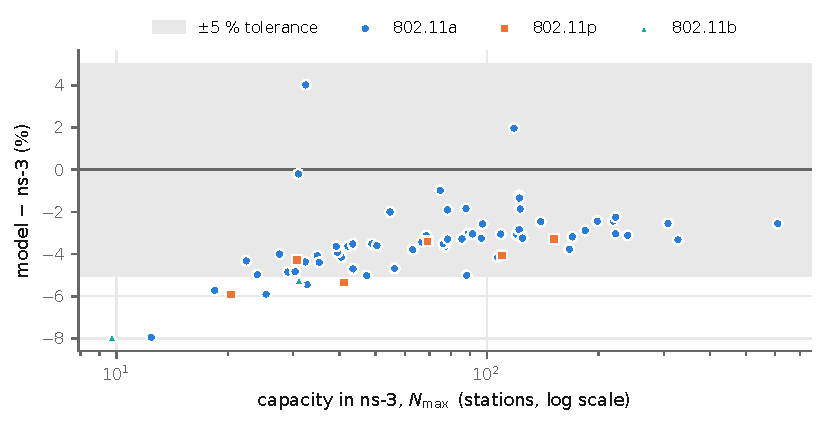
\includegraphics[width=\textwidth]{fig_scorecard}
\caption{The root of \eqref{eq:G5} against \scRows{} capacities stored from ns-3. Below zero, the
model under-predicts the capacity (the safe side).}
\label{fig:scorecard}
\end{figure}

\subsection{The safe side, by traffic source (UJ)}\label{sec:uj}

UJ tested on two new 802.11a cells whether the root of \eqref{eq:G5} stays on the safe side when the
stations' timers jitter or drift, and what frozen phases do (\cref{fig:uj}). It was registered with
two claims for the five non-frozen cells: S, the root at or below ns-3; A, the root and the law
within $\pm5\,\%$. \textbf{S held at all \ujSHeld{}}, the root's error \ujRootMax{} to \ujRootMin\,\%; A held at \ujAHeld, the two misses conservative. With frozen phases (strictly periodic senders,
identical clocks) ns-3's capacity fell by \ujFzDrop\,\% in both cells, to the root
(\ujFzRootMin{} and \ujFzRootMax\,\%) but not past it; the law, which lies slightly above the root,
was optimistic there (\ujFzLawMin{} to \ujFzLawMax\,\%). The registration's outcomes table sent that
case to Mohamed, who decided: \textbf{frozen phases are outside the safe-side claim}. The claim
the report makes is therefore: \emph{the root of \eqref{eq:G5} is on the safe side for timers with
jitter or clock drift} (all new cells, and all stored ones).

\begin{figure}[htbp]
\centering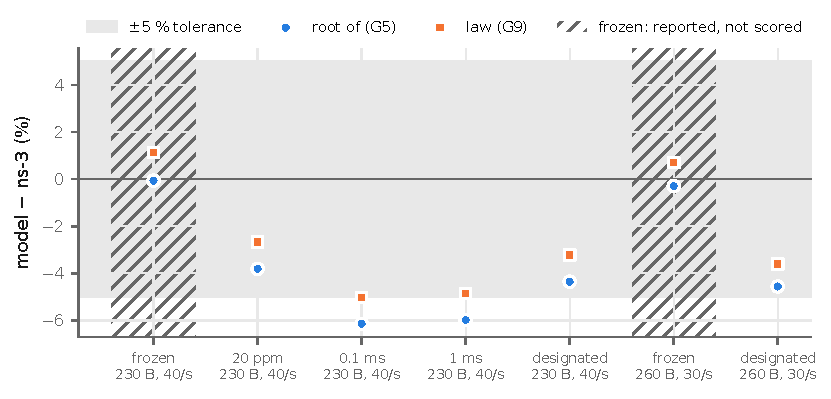
\includegraphics[width=\textwidth]{fig_uj}
\caption{UJ: the error of the root of \eqref{eq:G5} and of the law \eqref{eq:G9} against ns-3, by
traffic source, on two new 802.11a cells. Hatched: frozen phases, reported.}
\label{fig:uj}
\end{figure}

\iffull
\begin{table}[htbp]
\centering\footnotesize
% Generated by analysis/report_numbers.py from results/raw; do not edit by hand.
\begin{tabular}{lllrrllr}
\toprule
Cell & Source & ns-3 $\Nmax$ (95\,\% CI) & Root (\%) & Law (\%) & S & A & Seed $\sigma$ \\
\midrule
JA230F40 & frozen & 32.64 (30.85--33.77) & \textminus{}0.07 & +1.13 & reported & reported & 1.47 \\
JA230F40 & 20 ppm drift & 33.91 (31.64--34.43) & \textminus{}3.81 & \textminus{}2.66 & yes & yes & 1.61 \\
JA230F40 & jitter 0.1 ms & 34.75 (31.81--35.55) & \textminus{}6.14 & \textminus{}5.02 & yes & no & 1.46 \\
JA230F40 & jitter 1 ms & 34.69 (33.72--35.47) & \textminus{}5.98 & \textminus{}4.86 & yes & no & 1.19 \\
JA230F40 & designated & 34.10 (33.91--34.27) & \textminus{}4.36 & \textminus{}3.21 & yes & yes & 0.54 \\
JA260F30 & frozen & 40.09 (39.20--41.28) & \textminus{}0.30 & +0.70 & reported & reported & 1.47 \\
JA260F30 & designated & 41.88 (41.69--42.09) & \textminus{}4.56 & \textminus{}3.61 & yes & yes & 0.46 \\
\bottomrule
\end{tabular}

\caption{UJ in full (S: the root at or below ns-3; A: root and law within $\pm5\,\%$; seed $\sigma$:
the spread of each seed's own crossing).}
\end{table}
\fi

\subsection{The 802.11b arm, and why the sending pattern matters}

At the hardware's own PHY (802.11b, 1\,Mb/s), test UD found the Poisson model low at \udBelow{} of
its \udDOneAll{} small-swarm crossings. At 15--37 stations the root of \eqref{eq:G5} failed the
$\pm5\,\%$ band at \udDRootFailed{} of \udDCells{} cells, all on the safe side (\udDRootMax{} to
\udDRootMin\,\%); at 8--14 stations, with a band widened to $-9\ldots+5\,\%$ at registration, it held
at \udBHeld{} of \udBScored. Term by term, the loss itself was pessimistic by \udThreePMin{} to
\udThreePMax\,\% (D3); a capacity error is far smaller than a loss error because the loss rises
steeply with the load. The cause was the Poisson assumption: ns-3's telemetry source is periodic.
This failure is what \eqref{eq:G25} was written for.

\textbf{UD2 tested \eqref{eq:G25} where UD failed,} on new 802.11b cells at windows 8, 16 and 32 and
loss targets 2, 5 and 10\,\% (\cref{fig:ud2}). It held at all \udQHeld{} of \udQCrossings{}
crossings, with errors from \udQMin{} to \udQMax\,\%, including the \udQPast{} crossings past
occupancy 0.78. The Poisson root beside it erred by \udQPoiMin{} to \udQPoiMax\,\%, outside
$\pm5\,\%$ at \udQPoiOut: UD's failure, repeated on new cells and corrected by \eqref{eq:G25}. UD
itself stays failed as registered.

\begin{figure}[htbp]
\centering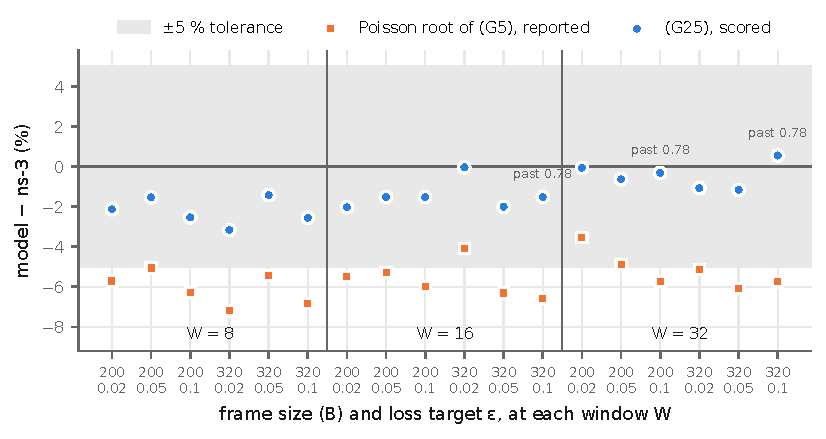
\includegraphics[width=\textwidth]{fig_ud2}
\caption{UD2: \eqref{eq:G25} (scored) and the Poisson root of \eqref{eq:G5} (reported) against
ns-3, 802.11b at 1\,Mb/s, two new frame sizes, three windows and three loss targets.}
\label{fig:ud2}
\end{figure}

\iffull
\begin{table}[htbp]
\centering\footnotesize
% Generated by analysis/report_numbers.py from results/raw; do not edit by hand.
\begin{tabular}{lrllrllr}
\toprule
Cell & $\Wnd$ & $\eps$ & ns-3 $\Nmax$ (95\,\% CI) & \eqref{eq:G25} & Error (\%) & Held & Poisson (\%) \\
\midrule
QB200F10W8 & 8 & 0.02 & 17.30 (17.11--17.44) & 16.93 & \textminus{}2.13 & yes & \textminus{}5.71 \\
QB200F10W8 & 8 & 0.05 & 24.82 (24.62--25.07) & 24.44 & \textminus{}1.54 & yes & \textminus{}5.06 \\
QB200F10W8 & 8 & 0.1 & 32.64 (32.46--32.81) & 31.81 & \textminus{}2.53 & yes & \textminus{}6.29 \\
QB320F8W8 & 8 & 0.02 & 15.47 (15.16--15.73) & 14.98 & \textminus{}3.16 & yes & \textminus{}7.20 \\
QB320F8W8 & 8 & 0.05 & 21.79 (21.60--22.06) & 21.48 & \textminus{}1.42 & yes & \textminus{}5.44 \\
QB320F8W8 & 8 & 0.1 & 28.60 (28.41--28.81) & 27.87 & \textminus{}2.55 & yes & \textminus{}6.82 \\
QB200F10W16 & 16 & 0.02 & 21.62 (21.33--22.08) & 21.18 & \textminus{}2.03 & yes & \textminus{}5.47 \\
QB200F10W16 & 16 & 0.05 & 30.10 (29.85--30.28) & 29.64 & \textminus{}1.51 & yes & \textminus{}5.28 \\
QB200F10W16 & 16 & 0.1 & 37.85 (37.69--38.05) & 37.27 & \textminus{}1.52 & yes & \textminus{}5.97 \\
QB320F8W16 & 16 & 0.02 & 18.82 (18.37--19.31) & 18.82 & \textminus{}0.03 & yes & \textminus{}4.07 \\
QB320F8W16 & 16 & 0.05 & 26.68 (26.50--26.88) & 26.15 & \textminus{}2.00 & yes & \textminus{}6.31 \\
QB320F8W16 & 16 & 0.1 & 33.26 (33.07--33.41) & 32.76 & \textminus{}1.51 (past 0.78) & yes & \textminus{}6.60 \\
QB200F10W32 & 32 & 0.02 & 25.66 (25.44--25.98) & 25.65 & \textminus{}0.06 & yes & \textminus{}3.55 \\
QB200F10W32 & 32 & 0.05 & 34.83 (34.64--35.06) & 34.61 & \textminus{}0.63 & yes & \textminus{}4.88 \\
QB200F10W32 & 32 & 0.1 & 42.16 (42.07--42.23) & 42.03 & \textminus{}0.30 (past 0.78) & yes & \textminus{}5.72 \\
QB320F8W32 & 32 & 0.02 & 23.21 (22.82--23.45) & 22.96 & \textminus{}1.07 & yes & \textminus{}5.13 \\
QB320F8W32 & 32 & 0.05 & 31.07 (30.82--31.26) & 30.71 & \textminus{}1.16 & yes & \textminus{}6.08 \\
QB320F8W32 & 32 & 0.1 & 36.92 (36.81--37.08) & 37.13 & +0.56 (past 0.78) & yes & \textminus{}5.75 \\
\bottomrule
\end{tabular}

\caption{UD2 in full, scored at $\pm5\,\%$.}
\end{table}
\fi

\subsection{The sending pattern}

With Poisson sources the model is \ugPoiMin{} to \ugPoiMax\,\% low on the new cells of UG25.
\eqref{eq:G25} was registered on those \ugCells{} cells and held at all \ugHeld{} (\ugMin{} to
\ugMax\,\%). Past occupancy 0.78 (\uhCells{} further cells at occupancy \uhOccMin--\uhOccMax) it is
optimistic by \uhMin{} to \uhMax\,\%, which is now a stated limit (\cref{fig:g25}).

\begin{figure}[htbp]
\centering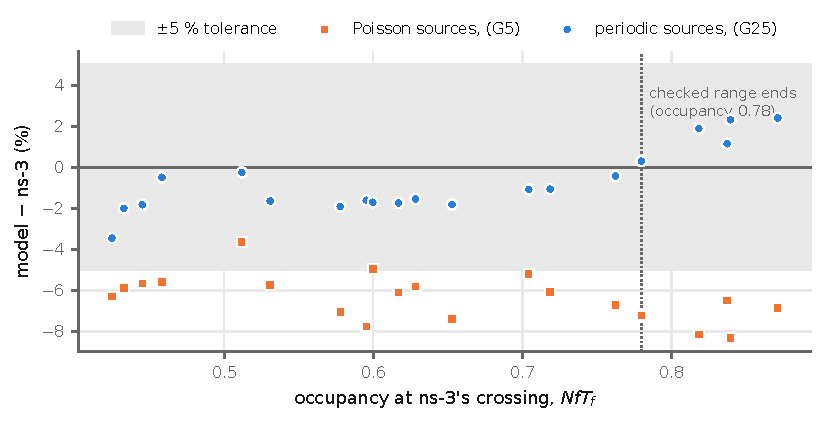
\includegraphics[width=\textwidth]{fig_g25}
\caption{The model's error against ns-3, with Poisson sources, \eqref{eq:G5}, and with periodic
sources, \eqref{eq:G25}, against the occupancy at which ns-3 reaches the loss target.}
\label{fig:g25}
\end{figure}

\subsection{Few stations}

For three to five stations the finite-station form \eqref{eq:FS} held at all \fsHeld{} of \fsCells{}
registered cells, with a tolerance of $\pm15\,\%$ on the loss (\cref{fig:fewstations}). The Poisson
loss \eqref{eq:G5} overstates the loss there by \fsGFiveMin--\fsGFiveMax\,\%.

\begin{figure}[htbp]
\centering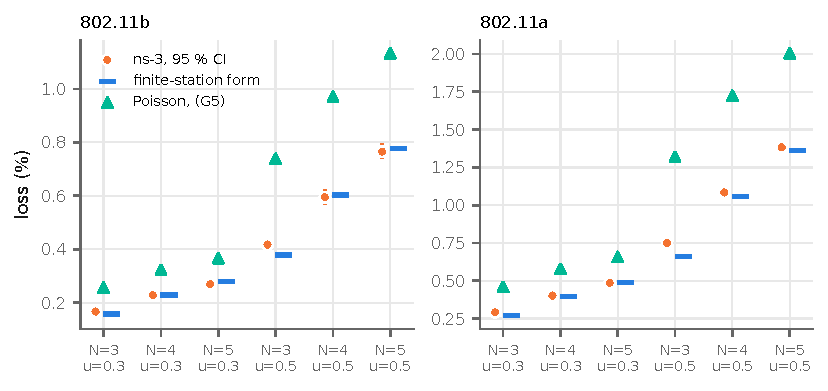
\includegraphics[width=\textwidth]{fig_fewstations}
\caption{UFS: the loss at three to five stations and occupancy 0.3 and 0.5, in ns-3 (30 seeds, 95\,\%
interval), by the finite-station form \eqref{eq:FS} and by the Poisson loss \eqref{eq:G5}.}
\label{fig:fewstations}
\end{figure}

\subsection{Batching}

The gain of batching \eqref{eq:G12} matched ns-3 within \gainMaxAbs\,\% at 802.11a up to 64 records
per frame, and within \gainBMaxAbs\,\% at 802.11b up to 32 (\cref{fig:batching}; reported beside
registered capacity tests UC2 and UD, whose capacities held \ucTwoHeld{} of \ucTwoClaims{} and
\udTwoHeld{} of \udTwoCells).

\begin{figure}[htbp]
\centering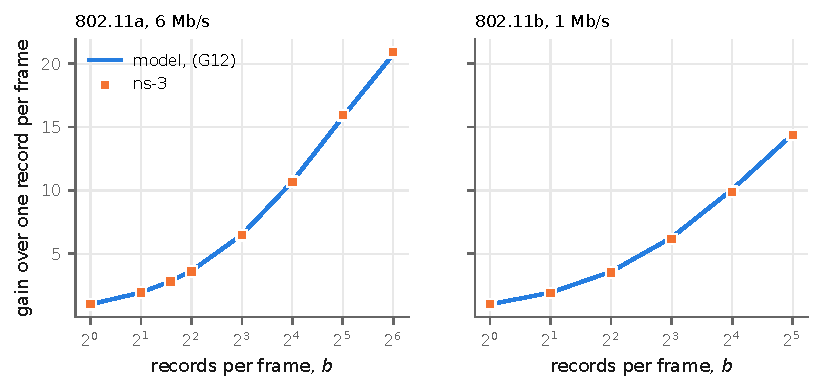
\includegraphics[width=\textwidth]{fig_batching}
\caption{The gain of batching: capacity at $b$ records per frame over capacity at one, less one
station each, \eqref{eq:G12} against ns-3.}
\label{fig:batching}
\end{figure}

\subsection{Capture}

ns-3's capture rule, read from its source and predicted per collision, held at \capHeld{} of
\capTrials{} offsets and power differences (UCAP2). A first capacity test with capture (UF) held
\ufAvgHeld{} of \ufConfigs{} average-delivery claims and only \ufWorstHeld{} of \ufConfigs{}
every-sender claims. Its three causes were found: the half-duplex factor \eqref{eq:G22a} was missing,
the every-sender claim had been scored on a sample minimum rather than on \eqref{eq:G24} or
\eqref{eq:G24a}, and one configuration had a station at the edge of carrier sense. The corrected
test UF2, on new placements and seeds, held all \ufTwoHeld{} of its \ufTwoClaims{} claims, every one
on the safe side: \eqref{eq:G23} within \ufTwoAMin{} to \ufTwoAMax\,\%, the pooled \eqref{eq:G24}
within \ufTwoPoolMin{} to \ufTwoPoolMax\,\%, the window statistic \eqref{eq:G24a} within
\ufTwoWinMin{} to \ufTwoWinMax\,\% (\cref{fig:uf2}).

\begin{figure}[htbp]
\centering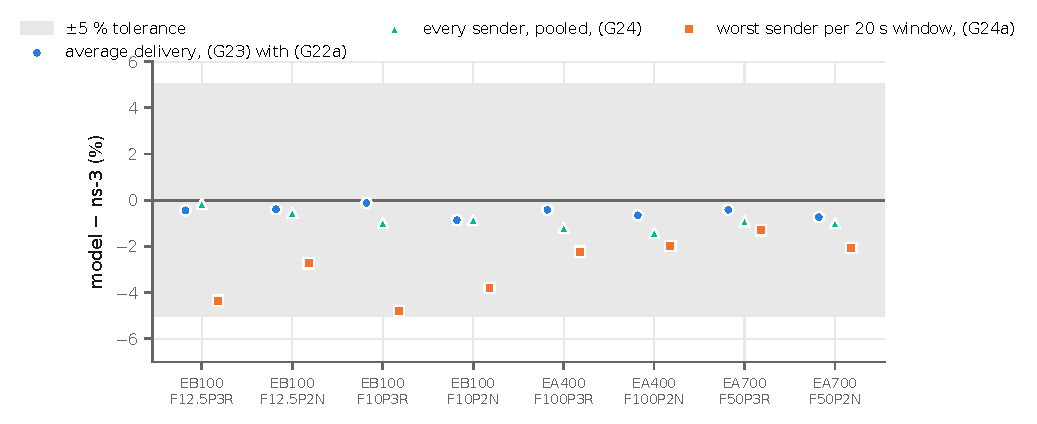
\includegraphics[width=\textwidth]{fig_uf2}
\caption{UF2: the capture laws against ns-3, per configuration (EB: 802.11b, EA: 802.11a; F: frames
per second; P3R: path-loss exponent 3 with Rayleigh fading; P2N: exponent 2, no fading).}
\label{fig:uf2}
\end{figure}

\subsection{Design rules and LoRa}

A key record once in $r=2$ or 4 frames held \ucThreeHeld{} of \ucThreeCells{} (UC3). Fragments spread
over the period held \ucFourSHeld{} of \ucFourSCells{} (UC4S); fragments sent back to back failed
(UC4), and a correction for them removed \burstFixMin--\burstFixMax\,\% of the excess but failed its
own test (UC4B), so the design forbids back-to-back fragments. The best batch under bit errors
\eqref{eq:G19} was predicted as \ucFivePred{} and ns-3's best was \ucFiveBest{} (UC5D1). The LoRa
duty-cycle law held at \lrHeld{} of \lrCells{} cells (UC7).

\subsection{What failed in simulation}

\begin{itemize}
\item \textbf{The split of \eqref{eq:G5} into its three causes} (UC1, D3): the totals hold, the
breakdown does not; ns-3 counts a near-simultaneous start as a detection-window loss.
\item \textbf{Poisson starts at 802.11b} (UD): the capacity \udDRootMax{} to \udDRootMin\,\% low at
15--37 stations; \eqref{eq:G25} then held at all \udQCrossings{} new crossings of UD2.
\item \textbf{The first capture test} (UF): failed for three identified reasons; the corrected test
held on new cells.
\item \textbf{Fragments sent back to back} (UC4, UC4B): outside the model; ruled out by design.
\item \textbf{\eqref{eq:G25} past occupancy 0.78 at 802.11b}: optimistic by \uhMin{} to \uhMax\,\%;
a stated limit.
\item \textbf{Frozen phases} (UJ and the stored cells): ns-3's capacity falls by about
\ujFzDrop\,\%, to the root or past it, and the law is optimistic there (stored: \scLawOptErr\,\%);
excluded from the safe-side claim.
\end{itemize}

% ==================================================================================================
\section{Validation on hardware}\label{sec:hw}
% ==================================================================================================

\textbf{What the hardware tests checked.} W1e, W1j and W1k were registered before the closed form
existed. Their predictions came from the project's event simulation of the DCF access rule
(registered at W1c), which had matched ns-3's capacities at 802.11b within \wOneBErr\,\% (W1b). They test
the access-rule model the closed form is built on, not the closed form's own numbers. W1r's
registration also recorded the closed form's values beside ns-3's; they are compared in
\cref{sec:side}. The first test of the closed form itself on the radios is V1a, below.

\subsection{The closed form on the radios (V1a)}\label{sec:v1a}

On three radios the part of the closed form that applies is the few-station form \eqref{eq:FS}
(three to five stations, occupancy up to 0.5). V1a scored it \emph{as stated}: the standard's window
$\Wnd=32$, rule set A, nothing measured on the radios. The three radios sent at occupancy 0.3, 0.4
and 0.5 in five interleaved rounds, with a control window after each; the session ran remotely and
every validity condition held (background \vaBg\,\%, each radio's link loss alone at most
\vaLinkMax\,\%). The registered tolerance was $\pm15\,\%$ on the loss.

\textbf{The closed form as stated failed at all \vaPoints{} points, on the optimistic side}
(\cref{fig:v1a,tab:v1a}). The radios lost \vaFacMin--\vaFacMax{} times what \eqref{eq:FS} predicts,
and the form lies below the 95\,\% interval of the measurement at every point. ns-3 and the event
simulation, both with the standard rule, sit near the form: the radios lose \vaSimMin--\vaSimMax{}
times what they predict. What misses is therefore the access rule the model assumes, not the
closed form's approximation of that rule. C1 measured the likely cause: the Pi~4s send about half
their frames at DIFS with no backoff, and the Pi~3 waits a fixed \cExtraC\,\us{} longer. A
hardware-matched form, with the radios' measured rule as its input, is the next registered test
(V1b, \cref{sec:next}). The failure was expected and disclosed in the registration; the stored trio
point of W1e and W1r had already pointed to it.

\begin{figure}[htbp]
\centering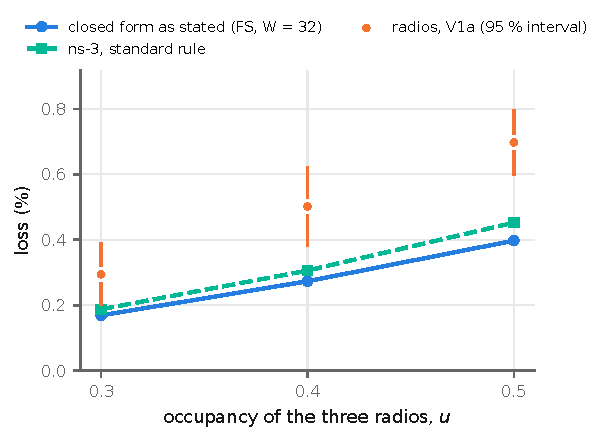
\includegraphics[width=0.66\textwidth]{fig_v1a}
\caption{V1a: the loss of the three radios against the closed form as stated, \eqref{eq:FS} at
$\Wnd=32$, and ns-3 with the standard rule.}
\label{fig:v1a}
\end{figure}

\begin{table}[htbp]
\centering\small
% Generated by analysis/report_numbers.py from results/raw; do not edit by hand.
\begin{tabular}{rrlrrlrrr}
\toprule
$\occ$ & $f$ & Radios, \% (95\,\% CI) & \eqref{eq:FS}, \% & Error (\%) & Held & ns-3, \% & Event sim., \% & \eqref{eq:G5}, \% \\
\midrule
0.3 & 52 & 0.294 (0.198--0.391) & \textbf{0.169} & \textminus{}42.7 & \textbf{no} & 0.188 & 0.193 & 0.263 \\
0.4 & 70 & 0.501 (0.378--0.625) & \textbf{0.273} & \textminus{}45.5 & \textbf{no} & 0.306 & 0.312 & 0.468 \\
0.5 & 87 & 0.697 (0.597--0.798) & \textbf{0.397} & \textminus{}43.0 & \textbf{no} & 0.452 & 0.446 & 0.743 \\
\bottomrule
\end{tabular}

\caption{V1a, scored at $\pm15\,\%$. The last three columns were reported, not scored;
\eqref{eq:G5} lies outside its stated range at three stations. Its closeness to the radios
(\vaGfiveMin{} to \vaGfiveMax\,\%) is not evidence for it: periodic sources make it pessimistic for
three stations, while the radios' rule adds collisions, so two departures act in opposite
directions; the matched form will separate them.}
\label{tab:v1a}
\end{table}

\subsection{Contention}

\Cref{fig:hw} shows the loss of two and three radios at occupancy 0.50, 0.70 and 0.85. In W1e (frame
burst on) \weHeld{} of \wePoints{} points lay inside the bands registered from the event
simulation; the miss was pi-A with pi-B at the lowest load, \weMissRatio{} times the prediction against a band
top of \weMissTop. In W1r (frame burst off) the hardware lies between two ns-3 settings of slot and
DIFS: inside the 95\,\% interval at \wrInTwenty{} of \wrPoints{} points for slot 20\,\us/DIFS
50\,\us, and \wrInNine{} for slot 9\,\us/DIFS 28\,\us. The pairs with the Pi 3 lose more than ns-3
predicts; ns-3 had been given windows inferred from each radio's sending rate, $\Wnd=\wrWinPi$ for
the Pi 4s and \wrWinPiThree{} for the Pi 3, and C1 later showed both to be wrong in kind
(\cref{sec:window}).

\begin{figure}[htbp]
\centering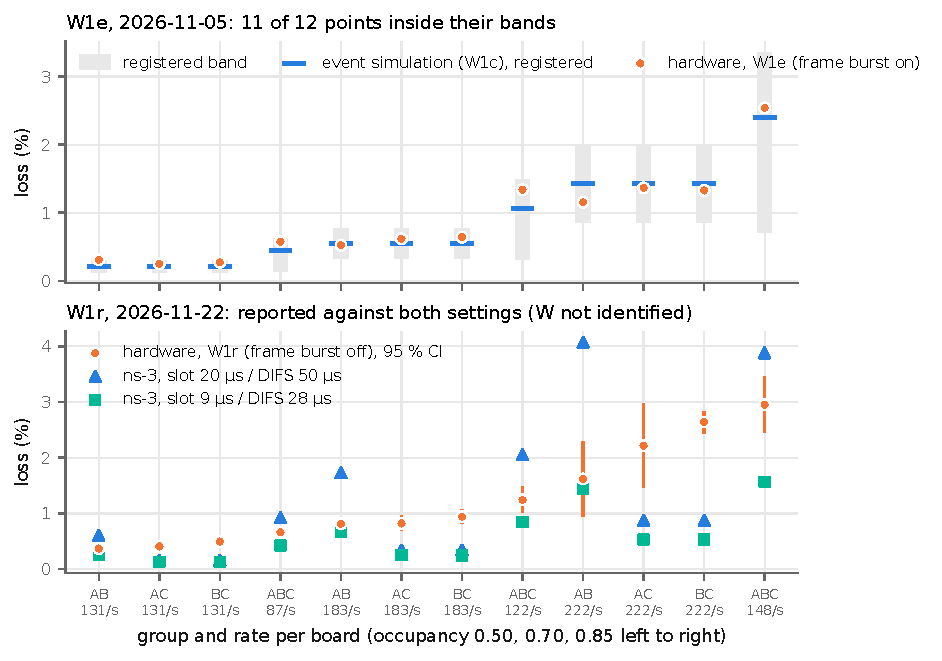
\includegraphics[width=\textwidth]{fig_hw_contention}
\caption{Hardware contention. Top: W1e against its registered prediction (the event simulation of
W1c). Bottom: W1r against ns-3 with two settings of slot and DIFS (the contention window was not
known; \cref{sec:window}).}
\label{fig:hw}
\end{figure}

\subsection{The capacity ratio}

On four radios (pi-A, pi-B, the Pi 3 and the TP-Link), the capacity of the design (one signature per
frame of four records) divided by that of per-record signing was \ratioJ{} in W1j and \ratioK{} in
W1k, against the registered \ratioModel{} (band \ratioLo--\ratioHi; \cref{fig:ratio}). The capacities
themselves were \crossAuthJ{} and \crossPerJ{} capacity-equivalent stations in W1j, against
\crossAuthModel{} and \crossPerModel{} (\crossAuthErr{} and \crossPerErr\,\%), attributed in W1j
to capture at the receivers, while the ratio moved by \ratioErr\,\%.

\begin{figure}[htbp]
\centering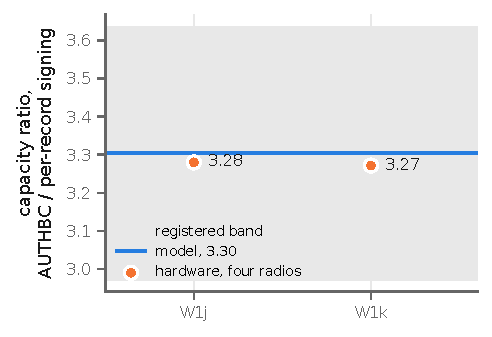
\includegraphics[width=0.5\textwidth]{fig_ratio}
\caption{The capacity ratio on four radios against the registered value.}
\label{fig:ratio}
\end{figure}

\subsection{Loss on air}

W3a traced every frame on air at 802.11b and replayed the traces through the project's real
decoder. All \wtHeld{} of \wtClaims{} registered claims held: real loss hurts the frames that depend
on a key record no more than independent loss would; the design loses only its own frames; and the
loss grows with frame length less steeply than a bit-error model predicts.

\subsection{Capture}

In W1q (the Pi 3 receiving, pi-A's power stepped) \wqHeld{} of \wqScored{} registered predictions
held. The one that failed is the finding: at a measured difference of only \wqThreeDelta\,dB the Pi
3 kept the stronger frame in \wqThreeQ{} of collisions, where ns-3's rule keeps none below 4\,dB.
Capture on this radio is gradual, not a step. Three of W1q's five power steps were void because the
received signal fell by less than the set power (\cref{sec:window}). W1s then tested the gradual
curve on new power steps: \wsCurveHeld{} of \wsCurveScored{} held, so the curve is not used; the
boards' radio geometry had changed between the sessions (\cref{fig:capture}).

\begin{figure}[htbp]
\centering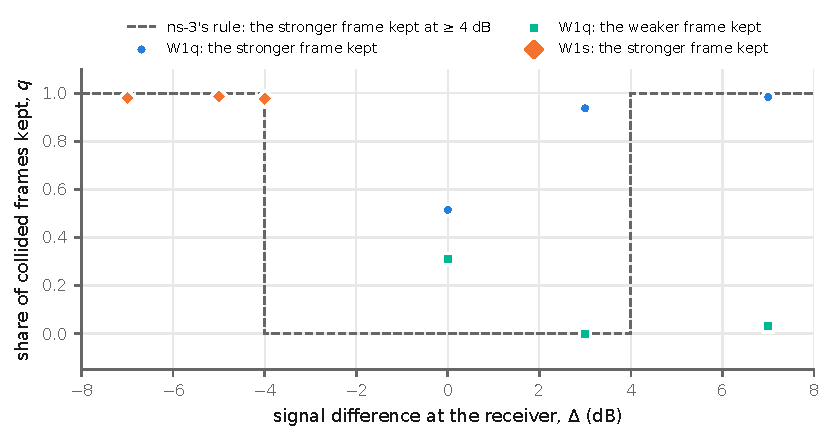
\includegraphics[width=\textwidth]{fig_capture_hw}
\caption{The share of collided frames the receiver kept, against the signal difference. Dashed:
ns-3's 4\,dB rule. W1q's points are from its valid steps; W1s's from its new steps.}
\label{fig:capture}
\end{figure}

\subsection{The contention window, and the radios' own timing}\label{sec:window}

The model needs each radio's contention window $\Wnd$, slot and DIFS; radios do not report them.
\textbf{W1p} tested two settings derived from each radio's sending rate: a saturated pair lost
\wpLoss{} at \wpFps{} frames/s, against ns-3's \wpTwentyLoss{} and \wpNineLoss: neither fits.
\textbf{W1s} re-derived both settings once and tested them at a new frame length: the pair lost
\wsPairLoss{} at \wsPairFps{} frames/s, against \wsTwentyLoss{} and \wsNineLoss: neither fits again,
so the window is recorded as not identifiable without a frame sniffer.

A sniffer was therefore added (the TP-Link in monitor mode, with a one-line driver change that
exports the chip's per-frame hardware timestamp). Its gate S0 \textbf{failed}: it recorded \sgA,
\sgB{} and \sgC{} of the three radios' frames, against the 0.99 required, though the radios
themselves received almost all of them; the misses follow neither the board nor its place, and a
probe at another placement (P1) did not reach 0.99 either; its planned placements 3\,m and 5\,m
away have not run. The same gate showed that the received signal
falls by \sgFalls\,dB when pi-A's set power falls by 3, 6 and 9\,dB; the Pi 3 registered a similar
compression, so the transmitter is the more likely cause, but this is not established. The sniffer
is used for timing only, under a stated rule, until a better adapter arrives.

\textbf{C1 (calibration, not validation)} measured each radio alone with the sniffer's microsecond
timestamps (\cref{fig:c1}). For both Pi 4s the gap after a frame has a floor of \cFloorA\,\us{} (the
standard's DIFS) and a 20\,\us{} lattice (the standard's slot); \cShareMinA--\cShareMaxB{} of their
frames are sent at DIFS with no backoff, and the rest spread over \cWminA{} slots. Under the
standard's rule a saturated sender draws its backoff from $0\ldots\Wnd-1$ after every frame, so only
about $1/\Wnd$ of frames (3\,\% at $\Wnd=32$) would go out at DIFS. Departures of commercial 802.11b cards from the standard's backoff have been
measured before \cite{bianchi2007cards}. The share did not change with a
back-to-back sender (\cShareKA), so it is the radio's own behaviour, not the sending pattern. The
Pi 3's floor is \cFloorC\,\us{} (\cExtraC\,\us{} more than DIFS) and \cShareMinC--\cShareMaxC{} of its
frames skip the backoff, close to the standard's $1/\Wnd$, with \cWminC--\cWmaxC{} slots. Across
frame sizes the airtime grows by \cSlope\,\us{} per byte (1\,Mb/s), with an intercept of
\cInterA\,\us{} (the long preamble, 192\,\us, plus DIFS). These are inputs for a hardware-matched
model; nothing has yet been validated with them.

\begin{figure}[htbp]
\centering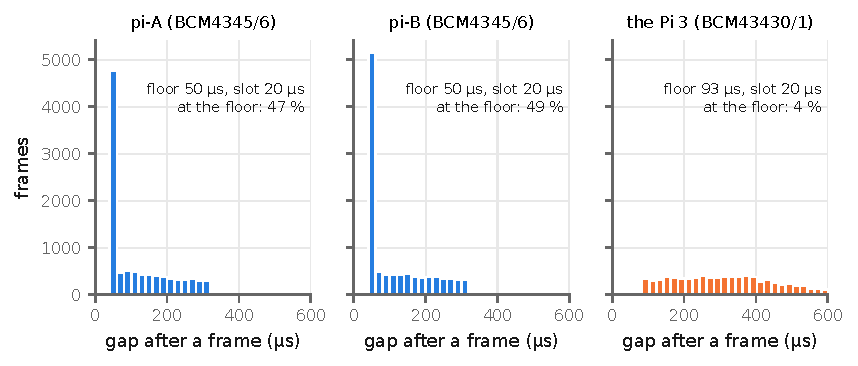
\includegraphics[width=\textwidth]{fig_c1_gaps}
\caption{C1: the gap after each frame, for each radio sending alone (145\,B frames). One bin per
backoff slot.}
\label{fig:c1}
\end{figure}

\iffull
\begin{figure}[htbp]
\centering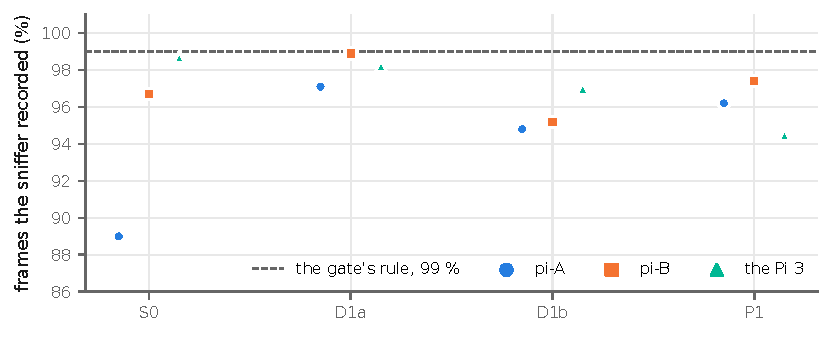
\includegraphics[width=\textwidth]{fig_sniffer}
\caption{The share of each radio's frames the sniffer recorded, session by session (S0: the gate;
D1a, D1b: diagnostics, pi-A and pi-B swapped in D1b; P1: the probe). The misses follow neither the
board nor its place.}
\label{fig:sniffer}
\end{figure}
\fi

\subsection{What failed on hardware}

\begin{itemize}
\item \textbf{The closed form as stated} (V1a): \eqref{eq:FS} at $\Wnd=32$ lies \vaErrB{} to
\vaErrA\,\% from the radios' loss at occupancy 0.3--0.5; the standard access rule is what differs.
\item \textbf{The window, from sending rates} (W1p, W1s): neither setting of slot and DIFS fits; the
window was not identifiable that way. C1 shows why: the Pi 4s skip the backoff for about half their
frames, which no single window describes.
\item \textbf{ns-3's 4\,dB capture step} (W1q): the radio captures at 1.5\,dB; the gradual curve
then failed its own check on new steps (W1s) after the geometry changed.
\item \textbf{The sniffer's gate} (S0, P1): the adapter misses \snifMissMin--\snifMissMax\,\% of frames, drifting between
sessions.
\item \textbf{Power steps}: the received signal falls by less than the set power, most likely at the
transmitter.
\end{itemize}

% ==================================================================================================
\section{Model, simulation and hardware side by side}\label{sec:side}
% ==================================================================================================

\Cref{tab:threeway} puts every source of a prediction beside the two hardware sessions, for the same
radios and rates: the closed forms (as recorded in W1r's registration, at the standard's
$\Wnd=32$), W1c's event simulation (W1e's registered prediction), ns-3 with two settings of slot and
DIFS, and the hardware with frame burst on (W1e) and off (W1r).

\begin{table}[htbp]
\centering\footnotesize
% Generated by analysis/report_numbers.py from results/raw; do not edit by hand.
\begin{tabular}{lrrrrrrrrrr}
\toprule
Radios & $\occ$ & $f$ & \eqref{eq:G5} & \eqref{eq:G25} & Finite & Event model & ns-3, $\slot=20$ & ns-3, $\slot=9$ & W1e & W1r \\
\midrule
AB & 0.50 & 131 & 0.41 & 0.30 & -- & 0.22 & 0.60 & 0.25 & 0.31 & 0.37 \\
AC & 0.50 & 131 & 0.41 & 0.30 & -- & 0.22 & 0.16 & 0.13 & 0.25 & 0.41 \\
BC & 0.50 & 131 & 0.41 & 0.30 & -- & 0.22 & 0.16 & 0.13 & 0.27 & 0.50 \\
ABC & 0.50 & 87 & 0.74 & 0.55 & 0.40 & 0.45 & 0.92 & 0.42 & 0.58 & 0.66 \\
AB & 0.70 & 183 & 0.83 & 0.54 & -- & 0.55 & 1.73 & 0.67 & 0.52 & 0.81 \\
AC & 0.70 & 183 & 0.83 & 0.54 & -- & 0.55 & 0.34 & 0.25 & 0.62 & 0.82 \\
BC & 0.70 & 183 & 0.83 & 0.54 & -- & 0.55 & 0.34 & 0.24 & 0.64 & 0.94 \\
ABC & 0.70 & 122 & 1.66 & 1.10 & -- & 1.06 & 2.05 & 0.84 & 1.34 & 1.24 \\
AB & 0.85 & 222 & 1.31 & 0.79 & -- & 1.43 & 4.07 & 1.44 & 1.15 & 1.62 \\
AC & 0.85 & 222 & 1.31 & 0.79 & -- & 1.43 & 0.87 & 0.53 & 1.37 & 2.21 \\
BC & 0.85 & 222 & 1.31 & 0.79 & -- & 1.43 & 0.87 & 0.53 & 1.33 & 2.64 \\
ABC & 0.85 & 148 & 2.82 & 1.69 & -- & 2.40 & 3.88 & 1.57 & 2.54 & 2.95 \\
\bottomrule
\end{tabular}

\caption{Loss (\%) of two and three radios, 802.11b at 1\,Mb/s, $f$ frames per second per radio.
For the pairs, \eqref{eq:G5} and \eqref{eq:G25} lie outside their stated range (two stations;
\eqref{eq:G25} needs 8 or more others); the finite-station form is shown only where it was accepted
(three stations, occupancy 0.5). The ns-3 values for the pairs with the Pi 3 use its inferred window
of \wrWinPiThree{} slots.}
\label{tab:threeway}
\end{table}

\textbf{What the comparison shows.}
\begin{itemize}
\item \textbf{The trio at occupancy 0.5}, the one point inside every model's range: \eqref{eq:FS},
the event simulation, ns-3 at slot 9\,\us{} and both hardware sessions lie between \twTrioLo{} and
\twTrioHi\,\%; \eqref{eq:G5} and ns-3 at slot 20\,\us{} lie above them.
\item \textbf{The pairs:} no closed form is claimed for two stations. ns-3's values for the pairs
with the Pi 3 are \twPiThreeLo--\twPiThreeHi{} times below the hardware, because ns-3 was given a window of
\wrWinPiThree{} slots for the Pi 3; C1 measured \cWminC--\cWmaxC{} plus a fixed \cExtraC\,\us.
\item \textbf{The same radios, two sessions} (W1e and W1r) differ by up to a factor of \twSessMax{} for the
pairs with the Pi 3: frame burst, placement and day all changed between them. A hardware number is a
property of a session, not only of the radios.
\end{itemize}

\begin{table}[htbp]
\centering\small
\begin{tabularx}{\textwidth}{>{\raggedright\arraybackslash}p{3.9cm}>{\raggedright\arraybackslash}p{2.4cm}>{\raggedright\arraybackslash}p{2.4cm}L}
\toprule
Quantity & Model & ns-3 & Hardware \\
\midrule
loss of three radios at $\occ=0.5$ (V1a) & \vaFinC\,\% \eqref{eq:FS} & \vaNsC\,\% (standard rule) & \vaLossC\,\% \\
capacity ratio, design over per-record signing (4 radios) & \ratioModel{} (event simulation) & -- & \ratioJ, \ratioK{} (W1j, W1k) \\
gain of batching, 802.11a, $b$ up to 64 & \eqref{eq:G12} & within \gainMaxAbs\,\% & not tested (V2) \\
capture at a signal difference of \wqThreeDelta\,dB & \eqref{eq:G22} with the input $q$ & $q=0$ (4\,dB rule) & $q=\wqThreeQ$ (W1q) \\
slot, DIFS & 20\,\us, 50\,\us{} (standard) & the same & 20\,\us, \cFloorA\,\us{} (Pi 4s); 20\,\us, \cFloorC\,\us{} floor (Pi 3) \\
frames sent at DIFS with no backoff, saturated & about $1/\Wnd$ (the standard's backoff after every frame) & not measured & \cShareMinA--\cShareMaxB{} (Pi 4s); \cShareMinC--\cShareMaxC{} (Pi 3) \\
airtime per byte at 1\,Mb/s & 8\,\us & 8\,\us & \cSlope\,\us{} (C1) \\
\bottomrule
\end{tabularx}
\caption{One quantity at a time: what the model assumes or predicts, what ns-3 does, what the radios
do.}
\label{tab:side}
\end{table}

% ==================================================================================================
\section{What remains to be tested}\label{sec:next}
% ==================================================================================================

\Cref{tab:coverage} maps each part of the model against where it has been tested.
\Cref{tab:next} lists the open tests, in the order they can run.

\begin{table}[htbp]
\centering\small
\begin{tabularx}{\textwidth}{>{\raggedright\arraybackslash}p{4.2cm}LL}
\toprule
Part of the model & ns-3 & Hardware \\
\midrule
accounting and batching, \eqref{eq:G1}--\eqref{eq:G3}, \eqref{eq:G10}--\eqref{eq:G13} & held (UC2, UD) & ratio held (W1j, W1k, event simulation); gain on air not tested (V2) \\
loss \eqref{eq:G4}--\eqref{eq:G5} & total held; split into causes failed (UC1) & as stated, \textbf{failed} (V1a, through \eqref{eq:FS}); the radios' access rule differs (C1) \\
two-constant law \eqref{eq:G6}--\eqref{eq:G9} & held where valid, \scLawIn{} of \scLawRows & not tested \\
design rules \eqref{eq:G16}--\eqref{eq:G21} & held (UC3, UC4S, UC5D1, UC7); back-to-back fragments failed & not tested \\
capture \eqref{eq:G22}--\eqref{eq:G24a} & held after correction (UCAP2, UF2) & the input $q$ measured, partly (W1q); in contention not tested (V3, V4) \\
sending pattern \eqref{eq:G25}, \eqref{eq:FS} & held to occupancy 0.78, and at 802.11b at every window and target (UD2); 3--5 stations held & \eqref{eq:FS} as stated \textbf{failed} (V1a); with the measured rule: V1b \\
hidden stations; two stations & not tested; no closed form & not tested \\
\bottomrule
\end{tabularx}
\caption{The coverage map: where each part of the model has been tested, and how it came out.}
\label{tab:coverage}
\end{table}

\begin{table}[htbp]
\centering\small
\begin{tabularx}{\textwidth}{>{\raggedright\arraybackslash}p{3.6cm}>{\raggedright\arraybackslash}p{1.9cm}L>{\raggedright\arraybackslash}p{2.9cm}}
\toprule
Test & Where & What it would show & Waits on \\
\midrule
S0b: the AR9271 sniffer's gate, beside the TP-Link & hardware & whether a second sniffer records $\ge99\,\%$ of frames; whether the power steps compress at the sender & the adapter (by 30 November 2026) \\
C1 in W1q's layout (L1); P1 at 3\,m and 5\,m & hardware & the timing of C1 where the capture sessions ran; whether distance lets the TP-Link reach 0.99 & Mohamed at the boards \\
C2: saturated pairs with the sniffer & hardware & the access rule two radios use under contention: who skips the backoff, and when & S0b \\
C3: the capture curve, both signs of the signal difference & hardware & $q$ against the signal difference for the real receiver & S0b \\
The parameter file & -- & the measured slot, DIFS, access rule, airtime and link losses, as one input set & C1--C3; Mohamed's review \\
The hardware-matched form: \eqref{eq:FS} with each radio's measured backoff and fixed delay, checked against the event simulation & model & the closed form with the radios' own rule, derived and checked before any test & Mohamed's acceptance of the derivation \\
V1b: the matched form on a new session of the three radios, as V1a & hardware & whether the closed form predicts the radios once it is given their rule & C2; the parameter file \\
V2: batching on air & hardware & the gain \eqref{eq:G12} on real radios & the parameter file \\
V3, V4: capture in contention; every-sender statistics & hardware & \eqref{eq:G22}--\eqref{eq:G24a} on real radios & C3 \\
Transmitter or receiver: does pi-A's output follow its set power? & hardware & where the power steps compress & an external receiver (HackRF) if S0b cannot separate them \\
Hidden stations & ns-3 & the term $2h\nu\Tf$ & outside the current scope \\
Two stations; fragments sent back to back & model & a closed form (none exists) & a derivation \\
\bottomrule
\end{tabularx}
\caption{The open tests. Calibration (C) sets the inputs; validation (V) tests predictions made from
them; no session does both.}
\label{tab:next}
\end{table}

If no suitable adapter is available by 30 November 2026, C2 and C3 use the receivers' logs, as W1p
and W1q did, with the sniffer for timing only, and the report of those sessions states the
limitation.

% ==================================================================================================
\section{Conclusions}
% ==================================================================================================

\begin{itemize}
\item \textbf{What can be claimed now.} The closed form predicts ns-3's capacity within $\pm5\,\%$ in
\scRootIn{} of \scRows{} stored cases, and its root lies on the safe side for every timer with jitter
or clock drift (UJ); frozen phases are excluded. Its extensions
for the sending pattern and for capture hold in registered ns-3 tests on new cells. On hardware, the
capacity ratio of the design over per-record signing matches the registered value (\ratioJ{}
against \ratioModel), and the access-rule model behind the closed form fell inside the registered
bands at \weHeld{} of \wePoints{} contention points.
\item \textbf{What cannot be claimed yet.} That the closed form predicts the radios' loss: as stated,
with the standard's access rule, it does not (V1a: the radios lose \vaFacMin--\vaFacMax{} times its
prediction, and ns-3 with the same rule misses alike); whether it does with the radios' measured
rule is the next test (V1b). That the model's access rule is the radios': the Pi 4s send about
half their frames with no backoff, which the standard's rule does not include. That ns-3's 4\,dB
capture step describes the real receiver: it captures gradually.
\item \textbf{Next.} The hardware-matched form (derived, then checked against the event simulation);
a sniffer that passes its gate and the calibration sessions C2 and C3; the parameter file for
review; then V1b and the validation sessions V2--V4 against the matched model and ns-3.
\end{itemize}

\iffull
\appendix
% ==================================================================================================
\section{Notation}
% ==================================================================================================
\begin{table}[htbp]
\centering\small
\begin{tabular}{ll}
\toprule
Symbol & Meaning \\
\midrule
$\Lam$ & records per second per station \\
$b$, $\bstar$, $\bM$ & batch (records per frame); the batch used; the largest that fits \\
$\Dmax$, $\Dnet$, $\Sq$ & deadline; deadline net of the delay $\Sq$ \\
$\Phi$, $\Psi$, $\Bud$ & cost per frame, cost per record, budget of a resource \\
$\Tf$ & a frame's airtime \\
$f$, $\nu$ & frames per second per station; start rate of the other stations, $(N-1)f$ \\
$\occ$ & occupancy, $N f\Tf$ \\
$\slot$, $\Difs$, $\Wnd$, $\delta$ & slot, DIFS, contention window, preamble-detection time \\
$\eps$, $\eps'$, $\epsw$ & loss target; with capture, average; with capture, every sender \\
$\rhostar$, $\tauzero$, $\tauhat$, $\kappa$ & the two constants of \eqref{eq:G9}; per-frame channel cost; $1-\eps/2$ \\
$\Kbar$, $a$, $\gamma$, $\eta$ & co-waiting frames; busy, gap and immediate-access loads \\
$\pcoll$, $q$, $\qeff$, $\ell$, $\ellbar$ & collision loss; capture probability; with the half-duplex factor; link loss; its average \\
$\Ninf$, $\beta$, $\Gain$ & capacity limit, half-gain batch, gain of batching \\
$\Rper$ & periodic-source ratio of \eqref{eq:G25} \\
$m$, $M$, $\pi$ & bystanders, co-waiting count and co-waiting probability of \eqref{eq:FS} \\
$z_N$ & expected maximum of $N$ standard normal draws \\
\bottomrule
\end{tabular}
\end{table}

% ==================================================================================================
\section{Failed attempts and corrections, kept visible}
% ==================================================================================================

\begin{itemize}
\item \textbf{UF (capture, first test).} \ufAvgHeld{} of \ufConfigs{} and \ufWorstHeld{} of
\ufConfigs{} held. Three causes, each found from logged state, not assumed: the half-duplex factor
\eqref{eq:G22a} had been omitted from both the law and its check script, so their agreement could not
reveal it; the every-sender claim had been scored on a sample minimum, an extreme that grows with
the number of senders, rather than on \eqref{eq:G24} or \eqref{eq:G24a}; one configuration placed a
station at the edge of carrier sense, outside one collision domain. UF stays failed; UF2 tested the
corrections on new placements and seeds.
\item \textbf{UC4B (a burst correction for back-to-back fragments).} Removed
\burstFixMin--\burstFixMax\,\% of the excess but failed on both scored cells, on the optimistic
side. Not used; the design rule forbids the case.
\item \textbf{UG25H: \eqref{eq:G25} at high occupancy.} An earlier estimate from capture runs put
the error at \fOneFortyMin--\fOneFortyMax\,\%; measured once without capture it is \uhMin{} to \uhMax\,\%. The band of
the earlier estimate held at none of the four cells.
\item \textbf{W1p and W1s (the window from sending rates).} Two re-derivations, two failures; by
Mohamed's rule no third attempt was made, and the window was recorded as not identifiable without a
sniffer.
\item \textbf{W1q's gradual capture curve.} Fitted after W1q's failure, then checked on new steps in
W1s: \wsCurveHeld{} of \wsCurveScored{}; not used.
\item \textbf{S0's timing criterion.} The registration compared the median of the sniffer's
start-to-start intervals with the receivers' mean cycle; with half the gaps at DIFS the median was
bound to fall below the mean. The means agree within \sZeroMeanMin--\sZeroMeanMax\,\%. A corrected gate (S0b) compares
mean with mean on new windows.
\item \textbf{C1's estimators.} Two estimators were revised after the gate's rate checks and before
C1 ran (the lattice had picked a harmonic; $\Wnd-1$ from a percentile read the long tail); both were
tested on synthetic gaps of known slot and window first, and the revision is disclosed in C1's
registration.
\end{itemize}

\FloatBarrier
% ==================================================================================================
\section{Every test, in full}
% ==================================================================================================

Each table is generated from the test's scored file in \texttt{results/raw/}.

\subsection{Simulation}

{\footnotesize\setlength{\tabcolsep}{3pt}
\renewcommand{\longcap}{Every stored ns-3 capacity against the law \eqref{eq:G9} and the root of
\eqref{eq:G5} (errors in \%; negative is the safe side; ``--'': the law is not valid for that
frame).\label{tab:scorecard}}
% Generated by analysis/report_numbers.py from results/raw; do not edit by hand.
\begin{longtable}{>{\raggedright}p{2.7cm}lclllr>{\raggedright}p{2.2cm}rrr}
\caption{\longcap}\\
\toprule
Source & Cell & Std & $\Wnd$ & $\eps$ & $f$ & $\Tf$ (\textmu s) & Jitter & ns-3 $\Nmax$ & Law (\%) & Root (\%) \\
\midrule\endfirsthead
\toprule
Source & Cell & Std & $\Wnd$ & $\eps$ & $f$ & $\Tf$ (\textmu s) & Jitter & ns-3 $\Nmax$ & Law (\%) & Root (\%) \\
\midrule\endhead
\bottomrule\endfoot
ns3\_\allowbreak{}nmax\_\allowbreak{}direct & A & a & 16 & 0.05 & 50 & 304 & 0/0ppm & 30.97 & +1.6 & \textminus{}0.2 \\
ns3\_\allowbreak{}nmax\_\allowbreak{}direct & A & a & 16 & 0.05 & 50 & 304 & 0.1/5000ppm & 32.69 & \textminus{}3.8 & \textminus{}5.5 \\
ns3\_\allowbreak{}nmax\_\allowbreak{}direct & A & a & 16 & 0.05 & 50 & 304 & 20/0ppm & 32.32 & \textminus{}2.6 & \textminus{}4.4 \\
ns3\_\allowbreak{}nmax\_\allowbreak{}direct & B & a & 16 & 0.05 & 12.5 & 472 & 0/0ppm & 87.76 & \textminus{}1.0 & \textminus{}1.8 \\
ns3\_\allowbreak{}nmax\_\allowbreak{}direct & B & a & 16 & 0.05 & 12.5 & 472 & 80/0ppm & 88.85 & \textminus{}2.2 & \textminus{}3.0 \\
ns3\_\allowbreak{}nmax\_\allowbreak{}direct & C & a & 16 & 0.05 & 50 & 268 & 0/0ppm & 32.41 & +6.4 & +4.0 \\
ns3\_\allowbreak{}nmax\_\allowbreak{}direct & C & a & 16 & 0.05 & 50 & 268 & 20/0ppm & 35.26 & \textminus{}2.2 & \textminus{}4.4 \\
ns3\_\allowbreak{}nmax\_\allowbreak{}direct & D & a & 16 & 0.05 & 12.5 & 304 & 0/0ppm & 118.3 & +3.9 & +2.0 \\
ns3\_\allowbreak{}nmax\_\allowbreak{}direct & D & a & 16 & 0.05 & 12.5 & 304 & 0.1/0ppm & 122.13 & +0.6 & \textminus{}1.2 \\
ns3\_\allowbreak{}nmax\_\allowbreak{}direct & D & a & 16 & 0.05 & 12.5 & 304 & 0.1/5000ppm & 122.92 & \textminus{}0.1 & \textminus{}1.9 \\
ns3\_\allowbreak{}nmax\_\allowbreak{}direct & D & a & 16 & 0.05 & 12.5 & 304 & 1/0ppm & 122.27 & +0.5 & \textminus{}1.3 \\
ns3\_\allowbreak{}nmax\_\allowbreak{}direct & D & a & 16 & 0.05 & 12.5 & 304 & 80/0ppm & 124.55 & \textminus{}1.4 & \textminus{}3.1 \\
ns3\_\allowbreak{}nmax\_\allowbreak{}direct & E & a & 16 & 0.05 & 12.5 & 828 & 0/0ppm & 54.74 & \textminus{}1.7 & \textminus{}2.0 \\
ns3\_\allowbreak{}nmax\_\allowbreak{}direct & E & a & 16 & 0.05 & 12.5 & 828 & 80/0ppm & 56.28 & \textminus{}4.4 & \textminus{}4.7 \\
ns3\_\allowbreak{}nmax\_\allowbreak{}direct & F & a & 16 & 0.05 & 12.5 & 568 & 0/0ppm & 74.75 & \textminus{}0.4 & \textminus{}1.0 \\
ns3\_\allowbreak{}nmax\_\allowbreak{}direct & F & a & 16 & 0.05 & 12.5 & 568 & 80/0ppm & 76.83 & \textminus{}3.1 & \textminus{}3.6 \\
ns3\_\allowbreak{}nmax\_\allowbreak{}direct & G & a & 16 & 0.05 & 12.5 & 572 & 80/0ppm & 76.26 & \textminus{}3.0 & \textminus{}3.5 \\
ns3\_\allowbreak{}nmax\_\allowbreak{}direct & H & a & 16 & 0.05 & 12.5 & 364 & 80/0ppm & 108.91 & \textminus{}1.8 & \textminus{}3.0 \\
ns3\_\allowbreak{}nmax\_\allowbreak{}direct & I & a & 16 & 0.05 & 12.5 & 456 & 80/0ppm & 91.34 & \textminus{}2.2 & \textminus{}3.0 \\
ns3\_\allowbreak{}nmax\_\allowbreak{}direct & RA & a & 16 & 0.05 & 20 & 304 & 50/0ppm & 78.35 & \textminus{}1.5 & \textminus{}3.3 \\
ns3\_\allowbreak{}nmax\_\allowbreak{}direct & RB & a & 16 & 0.05 & 5 & 472 & 200/0ppm & 219.19 & \textminus{}1.6 & \textminus{}2.4 \\
ns3\_\allowbreak{}nmax\_\allowbreak{}direct & RC & a & 16 & 0.05 & 20 & 268 & 50/0ppm & 85.58 & \textminus{}1.1 & \textminus{}3.3 \\
ns3\_\allowbreak{}nmax\_\allowbreak{}direct & RD & a & 16 & 0.05 & 5 & 304 & 200/0ppm & 307.95 & \textminus{}0.8 & \textminus{}2.5 \\
ns3\_\allowbreak{}nmax\_\allowbreak{}direct & SM & a & 16 & 0.05 & 50 & 200 & 20/0ppm & 42.15 & \textminus{}0.0 & \textminus{}3.6 \\
ns3\_\allowbreak{}nmax\_\allowbreak{}direct & ST & a & 16 & 0.05 & 50 & 216 & 20/0ppm & 40.44 & \textminus{}1.0 & \textminus{}4.1 \\
ns3\_\allowbreak{}nmax\_\allowbreak{}direct & SG & a & 16 & 0.05 & 50 & 224 & 20/0ppm & 39.44 & \textminus{}0.9 & \textminus{}3.9 \\
ns3\_\allowbreak{}nmax\_\allowbreak{}direct & SE & a & 16 & 0.05 & 50.5 & 268 & 19.802/0ppm & 34.81 & \textminus{}1.9 & \textminus{}4.1 \\
ns3\_\allowbreak{}nmax\_\allowbreak{}direct & SW & a & 16 & 0.05 & 50 & 356 & 20/0ppm & 29.0 & \textminus{}3.6 & \textminus{}4.8 \\
batch\_\allowbreak{}capacity & B2 & a & 16 & 0.05 & 25 & 280 & 40 & 66.73 & \textminus{}1.4 & \textminus{}3.4 \\
batch\_\allowbreak{}capacity & B3 & a & 16 & 0.05 & 16.6667 & 292 & 60 & 96.51 & \textminus{}1.3 & \textminus{}3.2 \\
batch\_\allowbreak{}capacity & B8 & a & 16 & 0.05 & 6.25 & 352 & 160 & 222.33 & \textminus{}1.7 & \textminus{}3.0 \\
design\_\allowbreak{}map\_\allowbreak{}validation & MB10 & a & 16 & 0.05 & 10 & 268 & 100 & 169.96 & \textminus{}0.9 & \textminus{}3.2 \\
design\_\allowbreak{}map\_\allowbreak{}validation & MD10-500 & a & 16 & 0.05 & 2.5 & 308 & 400 & 609.03 & \textminus{}0.8 & \textminus{}2.5 \\
design\_\allowbreak{}map\_\allowbreak{}validation & MB100 & a & 16 & 0.05 & 100 & 268 & 10 & 18.41 & \textminus{}3.7 & \textminus{}5.7 \\
design\_\allowbreak{}map\_\allowbreak{}validation & MD100-40 & a & 16 & 0.05 & 33.3333 & 292 & 30 & 48.9 & \textminus{}1.6 & \textminus{}3.5 \\
design\_\allowbreak{}map\_\allowbreak{}validation & MD100-500 & a & 16 & 0.05 & 2.0408 & 848 & 490 & 327.53 & \textminus{}3.1 & \textminus{}3.3 \\
design\_\allowbreak{}map\_\allowbreak{}validation & MB20 & a & 16 & 0.05 & 20 & 268 & 50 & 85.59 & \textminus{}1.1 & \textminus{}3.3 \\
design\_\allowbreak{}map\_\allowbreak{}validation & MB25 & a & 16 & 0.05 & 25 & 268 & 40 & 68.56 & \textminus{}0.9 & \textminus{}3.1 \\
design\_\allowbreak{}map\_\allowbreak{}validation & MB40 & a & 16 & 0.05 & 40 & 268 & 25 & 43.42 & \textminus{}1.3 & \textminus{}3.5 \\
design\_\allowbreak{}map\_\allowbreak{}validation & MD40-100 & a & 16 & 0.05 & 13.3333 & 292 & 75 & 120.15 & \textminus{}1.1 & \textminus{}3.1 \\
design\_\allowbreak{}map\_\allowbreak{}validation & C & a & 16 & 0.05 & 50 & 268 & 20 & 35.26 & \textminus{}2.2 & \textminus{}4.4 \\
design\_\allowbreak{}map\_\allowbreak{}validation & MD50-150 & a & 16 & 0.05 & 7.1429 & 340 & 140 & 198.59 & \textminus{}1.0 & \textminus{}2.4 \\
design\_\allowbreak{}map\_\allowbreak{}validation & MB75 & a & 16 & 0.05 & 75 & 268 & 13.3333 & 24.0 & \textminus{}2.9 & \textminus{}5.0 \\
design\_\allowbreak{}map\_\allowbreak{}validation & MD75-200 & a & 16 & 0.05 & 5.3571 & 424 & 186.667 & 222.61 & \textminus{}1.3 & \textminus{}2.2 \\
design\_\allowbreak{}map\_\allowbreak{}validation & D & a & 16 & 0.05 & 12.5 & 304 & 80 & 124.68 & \textminus{}1.5 & \textminus{}3.2 \\
design\_\allowbreak{}map\_\allowbreak{}validation & MD100-100 & a & 16 & 0.05 & 11.1111 & 364 & 90 & 122.12 & \textminus{}1.6 & \textminus{}2.8 \\
phy\_\allowbreak{}links & Pa6B & a & 16 & 0.05 & 50 & 268 & 1 period (run\_\allowbreak{}links.py) & 35.26 & \textminus{}2.2 & \textminus{}4.4 \\
phy\_\allowbreak{}links & Pa6D & a & 16 & 0.05 & 12.5 & 304 & 1 period (run\_\allowbreak{}links.py) & 124.68 & \textminus{}1.5 & \textminus{}3.2 \\
phy\_\allowbreak{}links & Pa12B & a & 16 & 0.05 & 50 & 144 & 1 period (run\_\allowbreak{}links.py) & 50.46 & -- & \textminus{}3.6 \\
phy\_\allowbreak{}links & Pa12D & a & 16 & 0.05 & 12.5 & 164 & 1 period (run\_\allowbreak{}links.py) & 184.22 & -- & \textminus{}2.9 \\
phy\_\allowbreak{}links & Pa24B & a & 16 & 0.05 & 50 & 84 & 1 period (run\_\allowbreak{}links.py) & 63.01 & -- & \textminus{}3.8 \\
phy\_\allowbreak{}links & Pa24D & a & 16 & 0.05 & 12.5 & 92 & 1 period (run\_\allowbreak{}links.py) & 239.65 & -- & \textminus{}3.1 \\
phy\_\allowbreak{}links & Pp3B & p & 16 & 0.05 & 50 & 536 & 1 period (run\_\allowbreak{}links.py) & 20.39 & \textminus{}4.9 & \textminus{}5.9 \\
phy\_\allowbreak{}links & Pp3D & p & 16 & 0.05 & 12.5 & 608 & 1 period (run\_\allowbreak{}links.py) & 69.13 & \textminus{}2.6 & \textminus{}3.4 \\
phy\_\allowbreak{}links & Pp6B & p & 16 & 0.05 & 50 & 288 & 1 period (run\_\allowbreak{}links.py) & 30.66 & \textminus{}1.0 & \textminus{}4.3 \\
phy\_\allowbreak{}links & Pp6D & p & 16 & 0.05 & 12.5 & 328 & 1 period (run\_\allowbreak{}links.py) & 109.64 & \textminus{}1.4 & \textminus{}4.1 \\
phy\_\allowbreak{}links & Pp12B & p & 16 & 0.05 & 50 & 168 & 1 period (run\_\allowbreak{}links.py) & 41.18 & -- & \textminus{}5.3 \\
phy\_\allowbreak{}links & Pp12D & p & 16 & 0.05 & 12.5 & 184 & 1 period (run\_\allowbreak{}links.py) & 151.62 & -- & \textminus{}3.3 \\
pq\_\allowbreak{}capacity & PQ1 & a & 16 & 0.05 & 50 & 1072 & 20 & 12.41 & \textminus{}7.8 & \textminus{}7.9 \\
pq\_\allowbreak{}capacity & PQ4 & a & 16 & 0.05 & 12.5 & 1108 & 80 & 43.5 & \textminus{}4.5 & \textminus{}4.7 \\
capacity\_\allowbreak{}97 & C & a & 16 & 0.03 & 50 & 268 & 20 & 27.56 & \textminus{}0.5 & \textminus{}4.0 \\
capacity\_\allowbreak{}97 & D & a & 16 & 0.03 & 12.5 & 304 & 80 & 97.3 & +0.4 & \textminus{}2.6 \\
w1a & C & a & 4 & 0.05 & 50 & 268 & 20 & 25.33 & \textminus{}5.1 & \textminus{}5.9 \\
w1a & D & a & 4 & 0.05 & 12.5 & 304 & 80 & 88.09 & \textminus{}4.3 & \textminus{}5.0 \\
w1a & C & a & 8 & 0.05 & 50 & 268 & 20 & 30.35 & \textminus{}3.3 & \textminus{}4.8 \\
w1a & D & a & 8 & 0.05 & 12.5 & 304 & 80 & 106.85 & \textminus{}2.8 & \textminus{}4.2 \\
w1b & Pb1B & b & 32 & 0.05 & 50 & 1648 & 1 period (run\_\allowbreak{}links.py) & 9.72 & \textminus{}8.2 & \textminus{}7.9 \\
w1b & Pb1D & b & 32 & 0.05 & 12.5 & 1864 & 1 period (run\_\allowbreak{}links.py) & 31.05 & \textminus{}5.5 & \textminus{}5.2 \\
ns3\_\allowbreak{}rule\_\allowbreak{}cw31 & C & a & 32 & 0.05 & 50 & 268 & 20 & 39.18 & \textminus{}1.3 & \textminus{}3.6 \\
ns3\_\allowbreak{}rule\_\allowbreak{}cw31 & D & a & 32 & 0.05 & 12.5 & 304 & 80 & 139.61 & \textminus{}0.6 & \textminus{}2.5 \\
ns3\_\allowbreak{}rule\_\allowbreak{}levels & C & a & 16 & 0.1 & 50 & 268 & 20 & 47.36 & \textminus{}4.2 & \textminus{}5.0 \\
ns3\_\allowbreak{}rule\_\allowbreak{}levels & D & a & 16 & 0.1 & 12.5 & 304 & 80 & 166.79 & \textminus{}3.1 & \textminus{}3.8 \\
ns3\_\allowbreak{}rule\_\allowbreak{}levels & C & a & 16 & 0.02 & 50 & 268 & 20 & 22.4 & -- & \textminus{}4.3 \\
ns3\_\allowbreak{}rule\_\allowbreak{}levels & D & a & 16 & 0.02 & 12.5 & 304 & 80 & 78.27 & +2.3 & \textminus{}1.9 \\
\end{longtable}

}

\begin{table}[htbp]
\centering\footnotesize
% Generated by analysis/report_numbers.py from results/raw; do not edit by hand.
\begin{tabular}{lllllrlrl}
\toprule
Item & Cell & $\Wnd$ & $\eps$ & ns-3 $\Nmax$ (95\,\% CI) & Law (\%) & & Root (\%) & \\
\midrule
D1 & Pb1B & 32 & 0.02 & 7.558 (7.486--7.647) & \textminus{}9.7 & not scored & \textminus{}9.6 & not scored \\
D1 & Pb1B & 32 & 0.05 & 9.718 (9.678--9.76) & \textminus{}8.2 & held & \textminus{}7.9 & held \\
D1 & Pb1B & 32 & 0.1 & 11.158 (11.141--11.174) & \textminus{}5.0 & held & \textminus{}4.8 & held \\
D1 & Pb1BW16 & 16 & 0.02 & 6.414 (6.352--6.476) & \textminus{}9.4 & not scored & \textminus{}9.5 & not scored \\
D1 & Pb1BW16 & 16 & 0.05 & 8.567 (8.527--8.609) & \textminus{}8.6 & held & \textminus{}8.6 & held \\
D1 & Pb1BW16 & 16 & 0.1 & 10.429 (10.406--10.452) & \textminus{}7.9 & held & \textminus{}7.8 & held \\
D1 & Pb1BW8 & 8 & 0.02 & 5.382 (5.321--5.444) & \textminus{}10.7 & not scored & \textminus{}10.8 & not scored \\
D1 & Pb1BW8 & 8 & 0.05 & 7.313 (7.269--7.353) & \textminus{}9.4 & not scored & \textminus{}9.4 & not scored \\
D1 & Pb1BW8 & 8 & 0.1 & 9.204 (9.159--9.246) & \textminus{}8.9 & held & \textminus{}8.9 & held \\
D1 & Pb1D & 32 & 0.02 & 23.089 (22.86--23.336) & \textminus{}5.1 & failed & \textminus{}5.0 & held \\
D1 & Pb1D & 32 & 0.05 & 31.031 (30.896--31.177) & \textminus{}5.4 & failed & \textminus{}5.2 & failed \\
D1 & Pb1D & 32 & 0.1 & 37.32 (37.224--37.408) & \textminus{}5.5 & failed & \textminus{}5.3 & failed \\
D1 & Pb1DW16 & 16 & 0.02 & 19.26 (18.985--19.567) & \textminus{}5.5 & failed & \textminus{}5.6 & failed \\
D1 & Pb1DW16 & 16 & 0.05 & 26.728 (26.476--27.003) & \textminus{}5.1 & failed & \textminus{}5.0 & failed \\
D1 & Pb1DW16 & 16 & 0.1 & 33.667 (33.558--33.779) & \textminus{}5.9 & failed & \textminus{}5.9 & failed \\
D1 & Pb1DW8 & 8 & 0.02 & 15.553 (15.29--15.802) & \textminus{}6.2 & failed & \textminus{}6.3 & failed \\
D1 & Pb1DW8 & 8 & 0.05 & 22.278 (22.066--22.515) & \textminus{}5.6 & failed & \textminus{}5.6 & failed \\
D1 & Pb1DW8 & 8 & 0.1 & 29.099 (28.971--29.213) & \textminus{}6.3 & failed & \textminus{}6.2 & failed \\
D2 & DB1 & 32 & 0.05 & 42.629 (42.453--42.812) & \textminus{}4.8 & held & \textminus{}4.4 & held \\
D2 & DB2 & 32 & 0.05 & 79.79 (79.396--80.307) & \textminus{}3.2 & held & \textminus{}2.9 & held \\
D2 & DB4 & 32 & 0.05 & 147.657 (146.607--148.428) & \textminus{}3.3 & held & \textminus{}3.1 & held \\
D2 & DB8 & 32 & 0.05 & 257.261 (255.266--258.363) & \textminus{}3.0 & held & \textminus{}2.8 & held \\
D2 & DB16 & 32 & 0.05 & 412.462 (409.324--415.933) & \textminus{}3.1 & held & \textminus{}2.9 & held \\
D2 & DB32 & 32 & 0.05 & 599.31 (586.78--604.118) & \textminus{}4.4 & held & \textminus{}4.4 & held \\
\bottomrule
\end{tabular}

\caption{UD, the 802.11b arm: D1, small swarms at three windows and loss targets (Pb1B: 8--14
stations, band $-9\ldots+5\,\%$, not scored below 8 stations; Pb1D: 15--37 stations, band
$\pm5\,\%$); D2, batches of 1--32 records.}
\end{table}

\begin{table}[htbp]
\centering\footnotesize
% Generated by analysis/report_numbers.py from results/raw; do not edit by hand.
\begin{tabular}{llllrrrl}
\toprule
Cell & Std & $\eps$ & ns-3 $\Nmax$ (95\,\% CI) & \eqref{eq:G25} & Error (\%) & Poisson (\%) & Held \\
\midrule
GB120F15 & b & 0.05 & 32.60 (32.467--32.762) & 32.25 & \textminus{}1.1 & \textminus{}5.2 & yes \\
GB120F15 & b & 0.02 & 23.69 (23.509--23.914) & 23.63 & \textminus{}0.2 & \textminus{}3.6 & yes \\
GB120F20 & b & 0.05 & 24.95 (24.808--25.079) & 24.69 & \textminus{}1.1 & \textminus{}6.1 & yes \\
GB120F20 & b & 0.02 & 18.43 (18.223--18.664) & 18.13 & \textminus{}1.6 & \textminus{}5.7 & yes \\
GB240F15 & b & 0.05 & 21.18 (21.046--21.291) & 21.09 & \textminus{}0.4 & \textminus{}6.7 & yes \\
GB240F15 & b & 0.02 & 16.05 (15.743--16.245) & 15.74 & \textminus{}1.9 & \textminus{}7.0 & yes \\
GB240F20 & b & 0.05 & 16.25 (16.166--16.319) & 16.30 & +0.3 & \textminus{}7.2 & yes \\
GB240F20 & b & 0.02 & 12.40 (12.239--12.558) & 12.20 & \textminus{}1.6 & \textminus{}7.8 & yes \\
GA640F20 & a & 0.05 & 32.31 (32.112--32.444) & 31.76 & \textminus{}1.7 & \textminus{}4.9 & yes \\
GA640F20 & a & 0.02 & 22.88 (22.399--23.157) & 22.09 & \textminus{}3.4 & \textminus{}6.3 & yes \\
GA640F30 & a & 0.05 & 22.16 (22.044--22.245) & 21.77 & \textminus{}1.7 & \textminus{}6.1 & yes \\
GA640F30 & a & 0.02 & 15.54 (15.349--15.706) & 15.23 & \textminus{}2.0 & \textminus{}5.9 & yes \\
GA900F20 & a & 0.05 & 24.70 (24.581--24.838) & 24.32 & \textminus{}1.5 & \textminus{}5.8 & yes \\
GA900F20 & a & 0.02 & 17.50 (17.318--17.718) & 17.18 & \textminus{}1.8 & \textminus{}5.7 & yes \\
GA900F30 & a & 0.05 & 17.11 (17.023--17.186) & 16.80 & \textminus{}1.8 & \textminus{}7.4 & yes \\
GA900F30 & a & 0.02 & 12.01 (11.855--12.201) & 11.95 & \textminus{}0.5 & \textminus{}5.6 & yes \\
LB200F40 & b & 0.05 & 9.84 (9.783--9.891) & 10.02 & +1.9 & \textminus{}8.2 & occ.\ 0.82 \\
LB300F30 & b & 0.05 & 9.72 (9.672--9.765) & 9.94 & +2.3 & \textminus{}8.3 & occ.\ 0.84 \\
LB120F30 & b & 0.08 & 19.38 (19.34--19.423) & 19.61 & +1.2 & \textminus{}6.5 & occ.\ 0.84 \\
LB173F30 & b & 0.08 & 15.58 (15.537--15.627) & 15.96 & +2.4 & \textminus{}6.9 & occ.\ 0.87 \\
\bottomrule
\end{tabular}

\caption{UG25: \eqref{eq:G25} on new cells, $\pm5\,\%$; last four rows, UG25H: 802.11b past
occupancy 0.78, measured, not scored.}
\end{table}

\begin{table}[htbp]
\centering\footnotesize
% Generated by analysis/report_numbers.py from results/raw; do not edit by hand.
\begin{tabular}{llrrrl}
\toprule
Configuration & Claim & ns-3 & Model & Error (\%) & Held \\
\midrule
EB100F12.5P3R & (a) (G23) with (G22a) & 48.52 & 48.31 & \textminus{}0.44 & yes \\
EB100F12.5P3R & statistic 2, (G24a) & 40.92 & 39.14 & \textminus{}4.35 & yes \\
EB100F12.5P3R & statistic 1, (G24) pooled & 46.41 & 46.34 & \textminus{}0.15 & yes \\
EB100F12.5P2N & (a) (G23) with (G22a) & 46.23 & 46.05 & \textminus{}0.39 & yes \\
EB100F12.5P2N & statistic 2, (G24a) & 38.28 & 37.24 & \textminus{}2.73 & yes \\
EB100F12.5P2N & statistic 1, (G24) pooled & 44.46 & 44.21 & \textminus{}0.55 & yes \\
EB100F10P3R & (a) (G23) with (G22a) & 59.87 & 59.79 & \textminus{}0.12 & yes \\
EB100F10P3R & statistic 2, (G24a) & 49.10 & 46.75 & \textminus{}4.79 & yes \\
EB100F10P3R & statistic 1, (G24) pooled & 57.53 & 56.97 & \textminus{}0.98 & yes \\
EB100F10P2N & (a) (G23) with (G22a) & 57.48 & 56.98 & \textminus{}0.86 & yes \\
EB100F10P2N & statistic 2, (G24a) & 46.18 & 44.42 & \textminus{}3.81 & yes \\
EB100F10P2N & statistic 1, (G24) pooled & 55.30 & 54.83 & \textminus{}0.86 & yes \\
EA400F100P3R & (a) (G23) with (G22a) & 11.98 & 11.93 & \textminus{}0.42 & yes \\
EA400F100P3R & statistic 2, (G24a) & 11.09 & 10.84 & \textminus{}2.22 & yes \\
EA400F100P3R & statistic 1, (G24) pooled & 11.27 & 11.13 & \textminus{}1.20 & yes \\
EA400F100P2N & (a) (G23) with (G22a) & 11.40 & 11.32 & \textminus{}0.66 & yes \\
EA400F100P2N & statistic 2, (G24a) & 10.54 & 10.33 & \textminus{}1.97 & yes \\
EA400F100P2N & statistic 1, (G24) pooled & 10.69 & 10.54 & \textminus{}1.41 & yes \\
EA700F50P3R & (a) (G23) with (G22a) & 14.93 & 14.86 & \textminus{}0.41 & yes \\
EA700F50P3R & statistic 2, (G24a) & 13.49 & 13.32 & \textminus{}1.30 & yes \\
EA700F50P3R & statistic 1, (G24) pooled & 14.05 & 13.92 & \textminus{}0.91 & yes \\
EA700F50P2N & (a) (G23) with (G22a) & 14.21 & 14.11 & \textminus{}0.74 & yes \\
EA700F50P2N & statistic 2, (G24a) & 12.96 & 12.69 & \textminus{}2.06 & yes \\
EA700F50P2N & statistic 1, (G24) pooled & 13.29 & 13.16 & \textminus{}0.98 & yes \\
\bottomrule
\end{tabular}

\caption{UF2: capacities (stations) with capture; (a) the average criterion \eqref{eq:G23} with
\eqref{eq:G22a}; statistic 1, the pooled every-sender loss \eqref{eq:G24}; statistic 2, the window
statistic \eqref{eq:G24a}. Tolerance $\pm5\,\%$.}
\end{table}

\begin{table}[htbp]
\centering\footnotesize
% Generated by analysis/report_numbers.py from results/raw; do not edit by hand.
\begin{tabular}{lllllrrrl}
\toprule
Cell & $N$ & $\occ$ & ns-3 loss, \% (95\,\% CI) & Finite (\%) & Error (\%) & \eqref{eq:G5} (\%) & \eqref{eq:G25} (\%) & Held \\
\midrule
FSB223N3U30 & 3 & 0.3 & 0.166 (0.151--0.183) & 0.158 & \textminus{}5.2 & +54.0 & +23.9 & yes \\
FSB223N3U50 & 3 & 0.5 & 0.417 (0.399--0.434) & 0.378 & \textminus{}9.3 & +77.1 & +28.7 & yes \\
FSB223N4U30 & 4 & 0.3 & 0.228 (0.208--0.246) & 0.229 & +0.4 & +41.4 & +17.2 & yes \\
FSB223N4U50 & 4 & 0.5 & 0.594 (0.567--0.624) & 0.603 & +1.4 & +63.2 & +22.7 & yes \\
FSB223N5U30 & 5 & 0.3 & 0.269 (0.248--0.289) & 0.280 & +4.1 & +36.2 & +15.5 & yes \\
FSB223N5U50 & 5 & 0.5 & 0.765 (0.739--0.795) & 0.778 & +1.7 & +48.1 & +14.4 & yes \\
FSA1031N3U30 & 3 & 0.3 & 0.292 (0.269--0.316) & 0.271 & \textminus{}7.1 & +57.5 & +24.9 & yes \\
FSA1031N3U50 & 3 & 0.5 & 0.750 (0.730--0.772) & 0.661 & \textminus{}11.9 & +75.9 & +26.9 & yes \\
FSA1031N4U30 & 4 & 0.3 & 0.402 (0.382--0.421) & 0.399 & \textminus{}0.8 & +43.9 & +18.1 & yes \\
FSA1031N4U50 & 4 & 0.5 & 1.085 (1.058--1.110) & 1.058 & \textminus{}2.5 & +58.9 & +19.1 & yes \\
FSA1031N5U30 & 5 & 0.3 & 0.486 (0.456--0.512) & 0.491 & +1.0 & +35.4 & +14.0 & yes \\
FSA1031N5U50 & 5 & 0.5 & 1.383 (1.345--1.424) & 1.363 & \textminus{}1.4 & +45.0 & +11.9 & yes \\
\bottomrule
\end{tabular}

\caption{UFS: the finite-station form \eqref{eq:FS} against ns-3's loss, tolerance $\pm15\,\%$; the
last two columns are the errors of \eqref{eq:G5} and \eqref{eq:G25}, reported.}
\end{table}

\begin{table}[htbp]
\centering\footnotesize
% Generated by analysis/report_numbers.py from results/raw; do not edit by hand.
\begin{tabular}{lrrrl}
\toprule
Cell & Model $\Nmax$ & ns-3 $\Nmax$ & ns-3 crossing & Held \\
\midrule
D0.1C1L20 & 26 & 25 & 25.76 & yes \\
D0.1C1L200 & 26 & 25 & 25.76 & yes \\
D0.1C3L20 & 78 & 75 & 75.77 & yes \\
D0.1C3L200 & 78 & 75 & 75.77 & yes \\
D0.1C8L20 & 206 & 206 & 201.37 & yes \\
D0.1C8L200 & 206 & 206 & 201.37 & yes \\
D1C1L20 & 3 & 2 & 2.91 & no \\
D1C1L200 & 3 & 2 & 2.91 & no \\
D1C3L20 & 8 & 8 & 8.05 & no \\
D1C3L200 & 8 & 8 & 8.05 & no \\
D1C8L20 & 21 & 22 & 20.78 & yes \\
D1C8L200 & 21 & 22 & 20.78 & yes \\
D10C1L20 & 1 & 1 & -- & yes \\
D10C1L200 & 1 & 1 & -- & yes \\
D10C3L20 & 1 & 2 & 2.70 & no \\
D10C3L200 & 1 & 1 & -- & yes \\
D10C8L20 & 3 & 5 & 5.44 & no \\
D10C8L200 & 3 & 3 & 3.36 & yes \\
\bottomrule
\end{tabular}

\caption{UC7: the LoRa duty-cycle law against ns-3's LoRaWAN module (D: duty cycle in \%; C:
channels; L: payload in bytes).}
\end{table}

\FloatBarrier
\subsection{Hardware}

\begin{table}[htbp]
\centering\footnotesize
% Generated by analysis/report_numbers.py from results/raw; do not edit by hand.
\begin{tabular}{lrrcl}
\toprule
Radios and rate & Measured loss (\%) & Model (\%) & Band (\%) & Held \\
\midrule
AB at 131/s & 0.311 & 0.217 & 0.130--0.304 & \textbf{no} \\
AB at 183/s & 0.524 & 0.552 & 0.331--0.773 & yes \\
AB at 222/s & 1.154 & 1.426 & 0.856--1.996 & yes \\
ABC at 87/s & 0.577 & 0.446 & 0.134--0.624 & yes \\
ABC at 122/s & 1.339 & 1.059 & 0.318--1.483 & yes \\
ABC at 148/s & 2.540 & 2.395 & 0.718--3.353 & yes \\
AC at 131/s & 0.251 & 0.217 & 0.130--0.304 & yes \\
AC at 183/s & 0.617 & 0.552 & 0.331--0.773 & yes \\
AC at 222/s & 1.367 & 1.426 & 0.856--1.996 & yes \\
BC at 131/s & 0.273 & 0.217 & 0.130--0.304 & yes \\
BC at 183/s & 0.642 & 0.552 & 0.331--0.773 & yes \\
BC at 222/s & 1.328 & 1.426 & 0.856--1.996 & yes \\
\bottomrule
\end{tabular}

\caption{W1e: contention, frame burst on; measured loss less the background, against the event
simulation registered at W1c.}
\end{table}

\begin{table}[htbp]
\centering\footnotesize
% Generated by analysis/report_numbers.py from results/raw; do not edit by hand.
\begin{tabular}{llll}
\toprule
Radios, rate (occupancy) & Hardware loss, \% (95\,\% CI) & ns-3, $\slot=20$ (\%) & ns-3, $\slot=9$ (\%) \\
\midrule
AB at 131/s (u = 0.5) & 0.369 (0.328--0.410) & 0.605 & 0.254 \\
AC at 131/s (u = 0.5) & 0.408 (0.349--0.467) & 0.156 & 0.129 \\
BC at 131/s (u = 0.5) & 0.495 (0.456--0.534) & 0.156 & 0.131 \\
ABC at 87/s (u = 0.5) & 0.662 (0.562--0.761) & 0.923--0.753 & 0.421--0.349 \\
AB at 183/s (u = 0.7) & 0.813 (0.728--0.897) & 1.730 & 0.668 \\
AC at 183/s (u = 0.7) & 0.821 (0.687--0.955) & 0.341 & 0.250 \\
BC at 183/s (u = 0.7) & 0.941 (0.817--1.064) & 0.341 & 0.244 \\
ABC at 122/s (u = 0.7) & 1.242 (1.010--1.474) & 2.053--1.742 & 0.845--0.728 \\
AB at 222/s (u = 0.85) & 1.619 (0.951--2.286) & 4.071 & 1.436 \\
AC at 222/s (u = 0.85) & 2.215 (1.465--2.965) & 0.874 & 0.530 \\
BC at 222/s (u = 0.85) & 2.640 (2.443--2.837) & 0.874 & 0.532 \\
ABC at 148/s (u = 0.85) & 2.951 (2.448--3.453) & 3.882--3.344 & 1.566--1.326 \\
\bottomrule
\end{tabular}

\caption{W1r: contention, frame burst off, against ns-3 with the windows inferred from sending
rates (for the trio, equal power to Rayleigh with capture).}
\end{table}

\begin{table}[htbp]
\centering\footnotesize
% Generated by analysis/report_numbers.py from results/raw; do not edit by hand.
\begin{tabular}{>{\raggedright}p{2.6cm}>{\raggedright}p{9.2cm}>{\raggedright\arraybackslash}p{2.6cm}}
\toprule
Step & Measured & Held \\
\midrule
0 dB (pi-A 15 dBm) & $\Delta$RSSI +5.0 dB; q\_A 0.985 (0.980-0.988), q\_B 0.030 (0.024-0.043); p\_A 0.1070, p\_B 0.0904; q\_A + q\_B 1.015 & weak True, strong True \\
3 dB (pi-A 12 dBm) & $\Delta$RSSI +1.5 dB; q\_A 0.937 (0.929-0.948), q\_B -0.001 (-0.019-0.009); p\_A 0.0995, p\_B 0.0834; q\_A + q\_B 0.936 & weak True, strong False \\
6 dB (pi-A 9 dBm) & $\Delta$RSSI +1.5 dB; q\_A 0.311 (0.273-0.352), q\_B 0.515 (0.487-0.539); p\_A 0.1095, p\_B 0.0836; q\_A + q\_B 0.826 & void (pi-A fell 3.5 dB, not 6 $\pm$ 1.5) \\
10 dB (pi-A 5 dBm) & $\Delta$RSSI +0.0 dB; q\_A -0.123 (-0.143--0.096), q\_B 0.856 (0.813-0.882); p\_A 0.0961, p\_B 0.0840; q\_A + q\_B 0.732 & void (pi-A fell 5.5 dB, not 10 $\pm$ 1.5) \\
15 dB (pi-A 0 dBm) & $\Delta$RSSI -4.5 dB; q\_A 0.277 (0.255-0.290), q\_B 0.896 (0.888-0.906); p\_A 0.1475, p\_B 0.0914; q\_A + q\_B 1.172 & void (pi-A fell 9.0 dB, not 15 $\pm$ 1.5) \\
\bottomrule
\end{tabular}

\caption{W1q: the capture steps as recorded (the Pi 3 receives; $q_A$, $q_B$: the share of
collided frames kept from pi-A and pi-B).}
\end{table}

\begin{table}[htbp]
\centering\footnotesize
% Generated by analysis/report_numbers.py from results/raw; do not edit by hand.
\begin{tabular}{>{\raggedright}p{2.6cm}>{\raggedright}p{9.2cm}>{\raggedright\arraybackslash}p{2.6cm}}
\toprule
Step & Measured & Held \\
\midrule
pi-A 15 dBm & $\Delta$ -5.0 dB; q\_A 0.055, q\_B 0.966; worst single-sender loss 0.27 \% & reported (drift) \\
pi-A 13 dBm & $\Delta$ -4.0 dB; q\_A 0.008, q\_B 0.978; worst single-sender loss 0.64 \% & True \\
pi-A 11 dBm & $\Delta$ -5.0 dB; q\_A 0.040, q\_B 0.986; worst single-sender loss 0.27 \% & True \\
pi-A 10 dBm & $\Delta$ -7.0 dB; q\_A -0.106, q\_B 0.980; worst single-sender loss 0.27 \% & False \\
pi-B 18 dBm, pi-A 15 dBm & $\Delta$ -4.0 dB; q\_A 0.018, q\_B 0.978; worst single-sender loss 1.09 \% & not scored (link) \\
\bottomrule
\end{tabular}

\caption{W1s, part A: the capture curve's new steps, as recorded.}
\end{table}

\begin{table}[htbp]
\centering\footnotesize
% Generated by analysis/report_numbers.py from results/raw; do not edit by hand.
\begin{tabular}{>{\raggedright}p{2.6cm}>{\raggedright}p{9.2cm}>{\raggedright\arraybackslash}p{2.6cm}}
\toprule
Step & Measured & Held \\
\midrule
pi-A, 1000 sent & 0.89 & False \\
pi-B, 1000 sent & 0.967 & reported \\
the Pi 3, 1000 sent & 0.987 & reported \\
00\_R1\_600fps & 9905 pairs; below 1864 us 0.00 \%; median 1934.0 us against the receivers' cycle 2049.8 us (5.65 \%) & False \\
01\_R2\_600fps & 10354 pairs; below 1864 us 0.00 \%; median 1934.0 us against the receivers' cycle 2117.7 us (8.67 \%) & False \\
02\_R3\_600fps & 8837 pairs; below 1864 us 0.00 \%; median 2203.0 us against the receivers' cycle 2483.0 us (11.28 \%) & False \\
12\_R1\_600fps & 10022 pairs; below 1864 us 0.00 \%; median 1954.0 us against the receivers' cycle 2037.4 us (4.09 \%) & False \\
13\_R2\_600fps & 10336 pairs; below 1864 us 0.00 \%; median 1934.0 us against the receivers' cycle 2093.7 us (7.63 \%) & False \\
14\_R3\_600fps & 8883 pairs; below 1864 us 0.00 \%; median 2213.0 us against the receivers' cycle 2455.1 us (9.86 \%) & False \\
3 dB down & 2.07 & True \\
6 dB down & 4.01 & False \\
9 dB down & 6.5 & False \\
\bottomrule
\end{tabular}

\caption{S0: the sniffer's gate, as recorded.}
\end{table}

\begin{table}[htbp]
\centering\footnotesize\setlength{\tabcolsep}{3.5pt}
% Generated by analysis/report_numbers.py from results/raw; do not edit by hand.
\begin{tabular}{llrrrrlrr}
\toprule
Window & Sender & Payload (B) & Recorded & Floor (\textmu s) & Lattice (\textmu s) & No backoff (strict) & $\Wnd-1$ & $>128$ slots (\%) \\
\midrule
00\_R1 & pi-A & 145 & 0.961 & 50 & 20 & 0.472 (0.469) & 13 & 0.03 \\
01\_R2 & pi-B & 145 & 0.978 & 50 & 20 & 0.483 (0.480) & 13 & 0.10 \\
02\_R3 & Pi 3 & 145 & 0.987 & 93 & 20 & 0.036 (0.036) & 20 & 0.64 \\
03\_Q1 & pi-A & 145 & 0.956 & 50 & 20 & 0.467 (0.465) & 13 & 0.05 \\
04\_Q1 & pi-A & 300 & 0.962 & 50 & 20 & 0.460 (0.468) & 13 & 0.00 \\
05\_Q1 & pi-A & 600 & 0.968 & 50 & 20 & 0.455 (0.453) & 13 & 0.03 \\
06\_Q1 & pi-A & 1000 & 0.959 & 50 & 20 & 0.447 (0.444) & 13 & 0.00 \\
11\_K1 & pi-A & 145 & 0.965 & 50 & 20 & 0.475 (0.479) & 13 & 0.00 \\
12\_Q2 & pi-B & 145 & 0.983 & 50 & 20 & 0.486 (0.486) & 13 & 0.02 \\
13\_Q2 & pi-B & 300 & 0.976 & 50 & 20 & 0.472 (0.474) & 13 & 0.15 \\
14\_Q2 & pi-B & 600 & 0.978 & 50 & 20 & 0.471 (0.469) & 13 & 0.34 \\
15\_Q2 & pi-B & 1000 & 0.963 & 50 & 20 & 0.451 (0.450) & 13 & 0.55 \\
20\_K2 & pi-B & 145 & 0.982 & 50 & 20 & 0.479 (0.480) & 13 & 0.16 \\
21\_Q3 & Pi 3 & 145 & 0.993 & 93 & 20 & 0.036 (0.036) & 22 & 1.73 \\
22\_Q3 & Pi 3 & 300 & 0.981 & 93 & 20 & 0.031 (0.031) & 25 & 3.93 \\
23\_Q3 & Pi 3 & 600 & 0.986 & 93 & 20 & 0.031 (0.030) & 24 & 4.36 \\
24\_Q3 & Pi 3 & 1000 & 0.955 & 93 & 20 & 0.039 (0.038) & 23 & 4.84 \\
29\_K3 & Pi 3 & 145 & 0.991 & 93 & 20 & 0.031 (0.030) & 24 & 2.48 \\
30\_R1 & pi-A & 145 & 0.966 & 50 & 20 & 0.467 (0.463) & 13 & 0.01 \\
31\_R2 & pi-B & 145 & 0.974 & 50 & 20 & 0.484 (0.484) & 13 & 0.69 \\
32\_R3 & Pi 3 & 145 & 0.990 & 93 & 20 & 0.033 (0.034) & 24 & 2.97 \\
\multicolumn{9}{l}{airtime fit, pi-A: slope 8.00\,\textmu s/B, intercept 242.0\,\textmu s} \\
\multicolumn{9}{l}{airtime fit, pi-B: slope 8.00\,\textmu s/B, intercept 242.0\,\textmu s} \\
\multicolumn{9}{l}{airtime fit, Pi 3: slope 8.00\,\textmu s/B, intercept 285.0\,\textmu s} \\
\bottomrule
\end{tabular}

\caption{C1 (calibration): each radio alone, saturated (R: rate checks; Q: redrawn sender at 600
frames/s; K: back-to-back). ``Recorded'': the sniffer's share of the frames sent; ``strict'': pairs
whose neighbours were also recorded. The 50 frames/s windows give link losses, not timing, and are
left out.}
\end{table}

\FloatBarrier
% ==================================================================================================
\section{Where every number comes from}
% ==================================================================================================
Every result in this report is a macro written by \texttt{analysis/report\_numbers.py} from the
project's stored results, or a cell of a table it generates. \Cref{tab:provenance} names each
macro's file and registration; \texttt{provenance.csv} beside this report holds the same list. The
figures are drawn by \texttt{analysis/report\_figures.py} from the same files. To rebuild:
\begin{verbatim}
python analysis/report_numbers.py
python analysis/report_figures.py
cd docs/reports/2026-11-27_model_report && ./build.sh
\end{verbatim}

{\footnotesize\setlength{\tabcolsep}{3pt}
\renewcommand{\longcap}{Every macro, its value, its file and its registration or meaning.\label{tab:provenance}}
% Generated by analysis/report_numbers.py from results/raw; do not edit by hand.
\begin{longtable}{>{\raggedright}p{3.0cm}>{\raggedright}p{2.0cm}>{\raggedright}p{4.6cm}>{\raggedright\arraybackslash}p{4.6cm}}
\caption{\longcap}\\
\toprule
Macro & Value & File & Registration or meaning \\
\midrule\endfirsthead
\toprule
Macro & Value & File & Registration or meaning \\
\midrule\endhead
\bottomrule\endfoot
\texttt{\textbackslash scRows} & 74 & \texttt{unified\_\allowbreak{}model\_\allowbreak{}vs\_\allowbreak{}ns3.csv} & analysis/\allowbreak{}score\_\allowbreak{}unified\_\allowbreak{}model.py \\
\texttt{\textbackslash scLawRows} & 67 & \texttt{unified\_\allowbreak{}model\_\allowbreak{}vs\_\allowbreak{}ns3.csv} & law\_\allowbreak{}valid rows \\
\texttt{\textbackslash scLawIn} & 62 & \texttt{unified\_\allowbreak{}model\_\allowbreak{}vs\_\allowbreak{}ns3.csv} & |err| $\le$ 5 \% \\
\texttt{\textbackslash scRootIn} & 64 & \texttt{unified\_\allowbreak{}model\_\allowbreak{}vs\_\allowbreak{}ns3.csv} & |err| $\le$ 5 \% \\
\texttt{\textbackslash scLawMeanAbs} & 2.3 & \texttt{unified\_\allowbreak{}model\_\allowbreak{}vs\_\allowbreak{}ns3.csv} & mean |err| \\
\texttt{\textbackslash scRootMeanAbs} & 3.6 & \texttt{unified\_\allowbreak{}model\_\allowbreak{}vs\_\allowbreak{}ns3.csv} & mean |err| \\
\texttt{\textbackslash scLawSafe} & 60 & \texttt{unified\_\allowbreak{}model\_\allowbreak{}vs\_\allowbreak{}ns3.csv} & err $\le$ 0 (model below ns-3) \\
\texttt{\textbackslash scRootSafe} & 72 & \texttt{unified\_\allowbreak{}model\_\allowbreak{}vs\_\allowbreak{}ns3.csv} & err $\le$ 0 \\
\texttt{\textbackslash scRootOut} & 10 & \texttt{unified\_\allowbreak{}model\_\allowbreak{}vs\_\allowbreak{}ns3.csv} & |err| > 5 \% \\
\texttt{\textbackslash scRootOutSafe} & 10 & \texttt{unified\_\allowbreak{}model\_\allowbreak{}vs\_\allowbreak{}ns3.csv} & err < -5 \% (conservative) \\
\texttt{\textbackslash scLawOut} & 5 & \texttt{unified\_\allowbreak{}model\_\allowbreak{}vs\_\allowbreak{}ns3.csv} & law: |err| > 5 \% \\
\texttt{\textbackslash scLawOutSafe} & 4 & \texttt{unified\_\allowbreak{}model\_\allowbreak{}vs\_\allowbreak{}ns3.csv} & law: err < -5 \% \\
\texttt{\textbackslash scLawOptN} & 1 & \texttt{unified\_\allowbreak{}model\_\allowbreak{}vs\_\allowbreak{}ns3.csv} & law: err > +5 \% (optimistic) \\
\texttt{\textbackslash scLawOptErr} & +6.4 & \texttt{unified\_\allowbreak{}model\_\allowbreak{}vs\_\allowbreak{}ns3.csv} & law: worst optimistic miss, cell C jitter 0/\allowbreak{}0ppm \\
\texttt{\textbackslash scARows} & 66 & \texttt{unified\_\allowbreak{}model\_\allowbreak{}vs\_\allowbreak{}ns3.csv} & 80211a \\
\texttt{\textbackslash scARootIn} & 60 & \texttt{unified\_\allowbreak{}model\_\allowbreak{}vs\_\allowbreak{}ns3.csv} & 80211a \\
\texttt{\textbackslash scARootMin} & \textminus{}7.9 & \texttt{unified\_\allowbreak{}model\_\allowbreak{}vs\_\allowbreak{}ns3.csv} & 80211a \\
\texttt{\textbackslash scARootMax} & +4.0 & \texttt{unified\_\allowbreak{}model\_\allowbreak{}vs\_\allowbreak{}ns3.csv} & 80211a \\
\texttt{\textbackslash scPRows} & 6 & \texttt{unified\_\allowbreak{}model\_\allowbreak{}vs\_\allowbreak{}ns3.csv} & 80211p \\
\texttt{\textbackslash scPRootIn} & 4 & \texttt{unified\_\allowbreak{}model\_\allowbreak{}vs\_\allowbreak{}ns3.csv} & 80211p \\
\texttt{\textbackslash scPRootMin} & \textminus{}5.9 & \texttt{unified\_\allowbreak{}model\_\allowbreak{}vs\_\allowbreak{}ns3.csv} & 80211p \\
\texttt{\textbackslash scPRootMax} & \textminus{}3.3 & \texttt{unified\_\allowbreak{}model\_\allowbreak{}vs\_\allowbreak{}ns3.csv} & 80211p \\
\texttt{\textbackslash scBRows} & 2 & \texttt{unified\_\allowbreak{}model\_\allowbreak{}vs\_\allowbreak{}ns3.csv} & 80211b \\
\texttt{\textbackslash scBRootIn} & 0 & \texttt{unified\_\allowbreak{}model\_\allowbreak{}vs\_\allowbreak{}ns3.csv} & 80211b \\
\texttt{\textbackslash scBRootMin} & \textminus{}7.9 & \texttt{unified\_\allowbreak{}model\_\allowbreak{}vs\_\allowbreak{}ns3.csv} & 80211b \\
\texttt{\textbackslash scBRootMax} & \textminus{}5.2 & \texttt{unified\_\allowbreak{}model\_\allowbreak{}vs\_\allowbreak{}ns3.csv} & 80211b \\
\texttt{\textbackslash ugCells} & 16 & \texttt{ug25\_\allowbreak{}scored.csv} & prereg-UG25 \\
\texttt{\textbackslash ugHeld} & 16 & \texttt{ug25\_\allowbreak{}scored.csv} & prereg-UG25 \\
\texttt{\textbackslash ugMin} & \textminus{}3.4 & \texttt{ug25\_\allowbreak{}scored.csv} & (G25) error \\
\texttt{\textbackslash ugMax} & +0.3 & \texttt{ug25\_\allowbreak{}scored.csv} & (G25) error \\
\texttt{\textbackslash ugPoiMin} & \textminus{}7.8 & \texttt{ug25\_\allowbreak{}scored.csv} & Poisson error \\
\texttt{\textbackslash ugPoiMax} & \textminus{}3.6 & \texttt{ug25\_\allowbreak{}scored.csv} & Poisson error \\
\texttt{\textbackslash uhCells} & 4 & \texttt{ug25h\_\allowbreak{}scored.csv} & prereg-UG25H \\
\texttt{\textbackslash uhMin} & +1.16 & \texttt{ug25h\_\allowbreak{}scored.csv} & (G25) error \\
\texttt{\textbackslash uhMax} & +2.41 & \texttt{ug25h\_\allowbreak{}scored.csv} & (G25) error \\
\texttt{\textbackslash uhOccMin} & 0.82 & \texttt{ug25h\_\allowbreak{}scored.csv} & occupancy at ns-3's crossing \\
\texttt{\textbackslash uhOccMax} & 0.87 & \texttt{ug25h\_\allowbreak{}scored.csv} & occupancy at ns-3's crossing \\
\texttt{\textbackslash capTrials} & 552 & \texttt{ucap2\_\allowbreak{}scored.csv} & prereg-UCAP2 \\
\texttt{\textbackslash capHeld} & 552 & \texttt{ucap2\_\allowbreak{}scored.csv} & prereg-UCAP2 \\
\texttt{\textbackslash ufConfigs} & 16 & \texttt{uf\_\allowbreak{}scored.csv} & prereg-UF \\
\texttt{\textbackslash ufAvgHeld} & 12 & \texttt{uf\_\allowbreak{}scored.csv} & (G23) \\
\texttt{\textbackslash ufWorstHeld} & 2 & \texttt{uf\_\allowbreak{}scored.csv} & (G24) \\
\texttt{\textbackslash ufTwoClaims} & 24 & \texttt{uf2\_\allowbreak{}scored.csv} & prereg-UF2 \\
\texttt{\textbackslash ufTwoHeld} & 24 & \texttt{uf2\_\allowbreak{}scored.csv} & prereg-UF2 \\
\texttt{\textbackslash ufTwoAMin} & \textminus{}0.86 & \texttt{uf2\_\allowbreak{}scored.csv} & (a) \\
\texttt{\textbackslash ufTwoAMax} & \textminus{}0.12 & \texttt{uf2\_\allowbreak{}scored.csv} & (a) \\
\texttt{\textbackslash ufTwoWinMin} & \textminus{}4.79 & \texttt{uf2\_\allowbreak{}scored.csv} & statistic 2 \\
\texttt{\textbackslash ufTwoWinMax} & \textminus{}1.30 & \texttt{uf2\_\allowbreak{}scored.csv} & statistic 2 \\
\texttt{\textbackslash ufTwoPoolMin} & \textminus{}1.41 & \texttt{uf2\_\allowbreak{}scored.csv} & statistic 1 \\
\texttt{\textbackslash ufTwoPoolMax} & \textminus{}0.15 & \texttt{uf2\_\allowbreak{}scored.csv} & statistic 1 \\
\texttt{\textbackslash fsCells} & 12 & \texttt{ufs\_\allowbreak{}scored.csv} & prereg-UFS \\
\texttt{\textbackslash fsHeld} & 12 & \texttt{ufs\_\allowbreak{}scored.csv} & prereg-UFS \\
\texttt{\textbackslash lrCells} & 18 & \texttt{uc7\_\allowbreak{}scored.csv} & prereg-UC7 \\
\texttt{\textbackslash lrHeld} & 12 & \texttt{uc7\_\allowbreak{}scored.csv} & prereg-UC7 \\
\texttt{\textbackslash gainMaxAbs} & 0.9 & \texttt{unified\_\allowbreak{}c2\_\allowbreak{}scored.csv} & batching gain (G12), reported, not scored \\
\texttt{\textbackslash ucTwoClaims} & 6 & \texttt{unified\_\allowbreak{}c2\_\allowbreak{}scored.csv} & prereg-UC2, law and root \\
\texttt{\textbackslash ucTwoHeld} & 6 & \texttt{unified\_\allowbreak{}c2\_\allowbreak{}scored.csv} & prereg-UC2, law and root \\
\texttt{\textbackslash udBScored} & 5 & \texttt{unified\_\allowbreak{}d\_\allowbreak{}scored.csv} & prereg-UD, Pb1B root \\
\texttt{\textbackslash udBHeld} & 5 & \texttt{unified\_\allowbreak{}d\_\allowbreak{}scored.csv} & prereg-UD, Pb1B root \\
\texttt{\textbackslash udDCells} & 9 & \texttt{unified\_\allowbreak{}d\_\allowbreak{}scored.csv} & prereg-UD, Pb1D \\
\texttt{\textbackslash udDRootFailed} & 8 & \texttt{unified\_\allowbreak{}d\_\allowbreak{}scored.csv} & prereg-UD, Pb1D root \\
\texttt{\textbackslash udDLawFailed} & 9 & \texttt{unified\_\allowbreak{}d\_\allowbreak{}scored.csv} & prereg-UD, Pb1D law \\
\texttt{\textbackslash udDRootMin} & \textminus{}6.3 & \texttt{unified\_\allowbreak{}d\_\allowbreak{}scored.csv} & Pb1D root error \\
\texttt{\textbackslash udDRootMax} & \textminus{}5.0 & \texttt{unified\_\allowbreak{}d\_\allowbreak{}scored.csv} & Pb1D root error \\
\texttt{\textbackslash udBelow} & 18 & \texttt{unified\_\allowbreak{}d\_\allowbreak{}scored.csv} & D1 crossings with the model below ns-3 \\
\texttt{\textbackslash udDOneAll} & 18 & \texttt{unified\_\allowbreak{}d\_\allowbreak{}scored.csv} & D1 crossings \\
\texttt{\textbackslash udTwoCells} & 6 & \texttt{unified\_\allowbreak{}d\_\allowbreak{}scored.csv} & prereg-UD, D2 \\
\texttt{\textbackslash udTwoHeld} & 6 & \texttt{unified\_\allowbreak{}d\_\allowbreak{}scored.csv} & prereg-UD, D2 law and root \\
\texttt{\textbackslash gainBMaxAbs} & 1.9 & \texttt{unified\_\allowbreak{}d\_\allowbreak{}scored.csv} & 802.11b gain (G12), reported \\
\texttt{\textbackslash ucOneHeld} & 17 & \texttt{unified\_\allowbreak{}c1\_\allowbreak{}scored.csv} & terms, a, K, p \\
\texttt{\textbackslash ucOneCases} & 48 & \texttt{unified\_\allowbreak{}c1\_\allowbreak{}scored.csv} & terms, a, K, p \\
\texttt{\textbackslash ucOnePHeld} & 7 & \texttt{unified\_\allowbreak{}c1\_\allowbreak{}scored.csv} & the total p \\
\texttt{\textbackslash ucOnePCases} & 8 & \texttt{unified\_\allowbreak{}c1\_\allowbreak{}scored.csv} & the total p \\
\texttt{\textbackslash ucOnePMin} & +2.5 & \texttt{unified\_\allowbreak{}c1\_\allowbreak{}scored.csv} & the total p: model against ns-3 (\%) \\
\texttt{\textbackslash ucOnePMax} & +13.2 & \texttt{unified\_\allowbreak{}c1\_\allowbreak{}scored.csv} & the total p: model against ns-3 (\%) \\
\texttt{\textbackslash udThreeHeld} & 18 & \texttt{unified\_\allowbreak{}d3\_\allowbreak{}scored.csv} & terms, a, K, p \\
\texttt{\textbackslash udThreeCases} & 48 & \texttt{unified\_\allowbreak{}d3\_\allowbreak{}scored.csv} & terms, a, K, p \\
\texttt{\textbackslash udThreePHeld} & 0 & \texttt{unified\_\allowbreak{}d3\_\allowbreak{}scored.csv} & the total p \\
\texttt{\textbackslash udThreePCases} & 8 & \texttt{unified\_\allowbreak{}d3\_\allowbreak{}scored.csv} & the total p \\
\texttt{\textbackslash udThreePMin} & +13.9 & \texttt{unified\_\allowbreak{}d3\_\allowbreak{}scored.csv} & the total p: model against ns-3 (\%) \\
\texttt{\textbackslash udThreePMax} & +44.3 & \texttt{unified\_\allowbreak{}d3\_\allowbreak{}scored.csv} & the total p: model against ns-3 (\%) \\
\texttt{\textbackslash ucThreeHeld} & 2 & \texttt{unified\_\allowbreak{}c34\_\allowbreak{}scored.csv} & prereg-UC3 \\
\texttt{\textbackslash ucThreeCells} & 2 & \texttt{unified\_\allowbreak{}c34\_\allowbreak{}scored.csv} & prereg-UC3 \\
\texttt{\textbackslash ucFourRootFailed} & 2 & \texttt{unified\_\allowbreak{}c34\_\allowbreak{}scored.csv} & prereg-UC4, back-to-back fragments \\
\texttt{\textbackslash ucFourCells} & 2 & \texttt{unified\_\allowbreak{}c34\_\allowbreak{}scored.csv} & prereg-UC4 \\
\texttt{\textbackslash ucFourSHeld} & 2 & \texttt{unified\_\allowbreak{}c4sb\_\allowbreak{}scored.csv} & prereg-UC4S, spread fragments \\
\texttt{\textbackslash ucFourSCells} & 2 & \texttt{unified\_\allowbreak{}c4sb\_\allowbreak{}scored.csv} & prereg-UC4S \\
\texttt{\textbackslash ucFiveBest} & 8 & \texttt{c5\_\allowbreak{}d1\_\allowbreak{}scored.csv} & prereg-UC5D1: ns-3's best batch \\
\texttt{\textbackslash ucFivePred} & 8 & \texttt{c5\_\allowbreak{}d1\_\allowbreak{}scored.csv} & prereg-UC5D1: the model's best batch \\
\texttt{\textbackslash wtHeld} & 3 & \texttt{w3a\_\allowbreak{}w3a\_\allowbreak{}2026-11-06.csv} & prereg-W3a \\
\texttt{\textbackslash wtClaims} & 3 & \texttt{w3a\_\allowbreak{}w3a\_\allowbreak{}2026-11-06.csv} & prereg-W3a \\
\texttt{\textbackslash weHeld} & 11 & \texttt{w1e\_\allowbreak{}w1e\_\allowbreak{}2026-11-05.csv} & prereg-W1e \\
\texttt{\textbackslash wePoints} & 12 & \texttt{w1e\_\allowbreak{}w1e\_\allowbreak{}2026-11-05.csv} & prereg-W1e \\
\texttt{\textbackslash ratioJ} & 3.28 & \texttt{w1i\_\allowbreak{}w1j\_\allowbreak{}2026-11-06\_\allowbreak{}run.csv} & AUTHBC /\allowbreak{} per-record, hardware \\
\texttt{\textbackslash ratioModel} & 3.30 & \texttt{w1i\_\allowbreak{}w1j\_\allowbreak{}2026-11-06\_\allowbreak{}run.csv} & AUTHBC /\allowbreak{} per-record, model \\
\texttt{\textbackslash ratioLo} & 2.97 & \texttt{w1i\_\allowbreak{}w1j\_\allowbreak{}2026-11-06\_\allowbreak{}run.csv} & registered band \\
\texttt{\textbackslash ratioHi} & 3.63 & \texttt{w1i\_\allowbreak{}w1j\_\allowbreak{}2026-11-06\_\allowbreak{}run.csv} & registered band \\
\texttt{\textbackslash crossAuthJ} & 30.5 & \texttt{w1i\_\allowbreak{}w1j\_\allowbreak{}2026-11-06\_\allowbreak{}run.csv} & AUTHBC crossing, hardware \\
\texttt{\textbackslash crossAuthModel} & 29.5 & \texttt{w1i\_\allowbreak{}w1j\_\allowbreak{}2026-11-06\_\allowbreak{}run.csv} & AUTHBC crossing, model \\
\texttt{\textbackslash crossPerJ} & 9.3 & \texttt{w1i\_\allowbreak{}w1j\_\allowbreak{}2026-11-06\_\allowbreak{}run.csv} & per-record crossing, hardware \\
\texttt{\textbackslash crossPerModel} & 8.9 & \texttt{w1i\_\allowbreak{}w1j\_\allowbreak{}2026-11-06\_\allowbreak{}run.csv} & per-record crossing, model \\
\texttt{\textbackslash ratioK} & 3.27 & \texttt{w1i\_\allowbreak{}w1k\_\allowbreak{}2026-11-06\_\allowbreak{}run.csv} & AUTHBC /\allowbreak{} per-record, hardware \\
\texttt{\textbackslash crossAuthK} & 30.7 & \texttt{w1i\_\allowbreak{}w1k\_\allowbreak{}2026-11-06\_\allowbreak{}run.csv} & AUTHBC crossing, hardware \\
\texttt{\textbackslash crossPerK} & 9.4 & \texttt{w1i\_\allowbreak{}w1k\_\allowbreak{}2026-11-06\_\allowbreak{}run.csv} & per-record crossing, hardware \\
\texttt{\textbackslash wpLoss} & 0.1029 & \texttt{w1p\_\allowbreak{}w1p\_\allowbreak{}2026-11-22.csv} & prereg-W1p \\
\texttt{\textbackslash wpFps} & 262.7 & \texttt{w1p\_\allowbreak{}w1p\_\allowbreak{}2026-11-22.csv} & prereg-W1p \\
\texttt{\textbackslash wpTwentyLoss} & 0.413 & \texttt{w1p\_\allowbreak{}w1p\_\allowbreak{}2026-11-22.csv} & ns-3 prediction \\
\texttt{\textbackslash wpTwentyFps} & 331 & \texttt{w1p\_\allowbreak{}w1p\_\allowbreak{}2026-11-22.csv} & ns-3 prediction \\
\texttt{\textbackslash wpNineLoss} & 0.169 & \texttt{w1p\_\allowbreak{}w1p\_\allowbreak{}2026-11-22.csv} & ns-3 prediction \\
\texttt{\textbackslash wpNineFps} & 288 & \texttt{w1p\_\allowbreak{}w1p\_\allowbreak{}2026-11-22.csv} & ns-3 prediction \\
\texttt{\textbackslash wqHeld} & 5 & \texttt{w1q\_\allowbreak{}w1q\_\allowbreak{}2026-11-22.csv + w1q\_\allowbreak{}w1q\_\allowbreak{}view.csv} & prereg-W1q \\
\texttt{\textbackslash wqScored} & 6 & \texttt{w1q\_\allowbreak{}w1q\_\allowbreak{}2026-11-22.csv + w1q\_\allowbreak{}w1q\_\allowbreak{}view.csv} & prereg-W1q \\
\texttt{\textbackslash wqThreeDelta} & 1.5 & \texttt{w1q\_\allowbreak{}w1q\_\allowbreak{}2026-11-22.csv} & the 3 dB step \\
\texttt{\textbackslash wqThreeQ} & 0.937 & \texttt{w1q\_\allowbreak{}w1q\_\allowbreak{}2026-11-22.csv} & the 3 dB step \\
\texttt{\textbackslash wrPoints} & 12 & \texttt{w1r\_\allowbreak{}w1r\_\allowbreak{}2026-11-22.csv} & prereg-W1r \\
\texttt{\textbackslash wrInTwenty} & 2 & \texttt{w1r\_\allowbreak{}w1r\_\allowbreak{}2026-11-22.csv} & slot 20 /\allowbreak{} DIFS 50 \\
\texttt{\textbackslash wrInNine} & 1 & \texttt{w1r\_\allowbreak{}w1r\_\allowbreak{}2026-11-22.csv} & slot 9 /\allowbreak{} DIFS 28 \\
\texttt{\textbackslash wsCurveHeld} & 2 & \texttt{w1s\_\allowbreak{}w1s\_\allowbreak{}2026-11-23.csv} & prereg-W1s, part A \\
\texttt{\textbackslash wsCurveScored} & 3 & \texttt{w1s\_\allowbreak{}w1s\_\allowbreak{}2026-11-23.csv} & prereg-W1s, part A \\
\texttt{\textbackslash wsPairLoss} & 0.1019 & \texttt{w1s\_\allowbreak{}w1s\_\allowbreak{}2026-11-23.csv} & prereg-W1s, part B \\
\texttt{\textbackslash wsPairFps} & 145.6 & \texttt{w1s\_\allowbreak{}w1s\_\allowbreak{}2026-11-23.csv} & prereg-W1s, part B \\
\texttt{\textbackslash wsTwentyLoss} & 0.1227 & \texttt{w1s\_\allowbreak{}w1s\_\allowbreak{}2026-11-23.csv} & ns-3, re-derived windows \\
\texttt{\textbackslash wsTwentyFps} & 149.5 & \texttt{w1s\_\allowbreak{}w1s\_\allowbreak{}2026-11-23.csv} & ns-3, re-derived windows \\
\texttt{\textbackslash wsNineLoss} & 0.0686 & \texttt{w1s\_\allowbreak{}w1s\_\allowbreak{}2026-11-23.csv} & ns-3, re-derived windows \\
\texttt{\textbackslash wsNineFps} & 145.9 & \texttt{w1s\_\allowbreak{}w1s\_\allowbreak{}2026-11-23.csv} & ns-3, re-derived windows \\
\texttt{\textbackslash wsD} & 158 & \texttt{w1s\_\allowbreak{}w1s\_\allowbreak{}2026-11-23.csv} & prereg-W1s, part C \\
\texttt{\textbackslash wsC} & 265 & \texttt{w1s\_\allowbreak{}w1s\_\allowbreak{}2026-11-23.csv} & prereg-W1s, part C \\
\texttt{\textbackslash sgA} & 0.890 & \texttt{s0\_\allowbreak{}s0\_\allowbreak{}2026-11-23.csv} & prereg-S0 \\
\texttt{\textbackslash sgB} & 0.967 & \texttt{s0\_\allowbreak{}s0\_\allowbreak{}2026-11-23.csv} & prereg-S0 \\
\texttt{\textbackslash sgC} & 0.987 & \texttt{s0\_\allowbreak{}s0\_\allowbreak{}2026-11-23.csv} & prereg-S0 \\
\texttt{\textbackslash sgFalls} & 2.1, 4.0, 6.5 & \texttt{s0\_\allowbreak{}s0\_\allowbreak{}2026-11-23.csv} & prereg-S0 \\
\texttt{\textbackslash cFloorA} & 50 & \texttt{c1\_\allowbreak{}c1\_\allowbreak{}2026-11-27.csv} & prereg-C1 (calibration) \\
\texttt{\textbackslash cShareMinA} & 0.45 & \texttt{c1\_\allowbreak{}c1\_\allowbreak{}2026-11-27.csv} & prereg-C1 \\
\texttt{\textbackslash cShareMaxA} & 0.47 & \texttt{c1\_\allowbreak{}c1\_\allowbreak{}2026-11-27.csv} & prereg-C1 \\
\texttt{\textbackslash cShareKA} & 0.47 & \texttt{c1\_\allowbreak{}c1\_\allowbreak{}2026-11-27.csv} & prereg-C1, back-to-back \\
\texttt{\textbackslash cWminA} & 13 & \texttt{c1\_\allowbreak{}c1\_\allowbreak{}2026-11-27.csv} & prereg-C1 \\
\texttt{\textbackslash cWmaxA} & 13 & \texttt{c1\_\allowbreak{}c1\_\allowbreak{}2026-11-27.csv} & prereg-C1 \\
\texttt{\textbackslash cFloorB} & 50 & \texttt{c1\_\allowbreak{}c1\_\allowbreak{}2026-11-27.csv} & prereg-C1 (calibration) \\
\texttt{\textbackslash cShareMinB} & 0.45 & \texttt{c1\_\allowbreak{}c1\_\allowbreak{}2026-11-27.csv} & prereg-C1 \\
\texttt{\textbackslash cShareMaxB} & 0.49 & \texttt{c1\_\allowbreak{}c1\_\allowbreak{}2026-11-27.csv} & prereg-C1 \\
\texttt{\textbackslash cShareKB} & 0.48 & \texttt{c1\_\allowbreak{}c1\_\allowbreak{}2026-11-27.csv} & prereg-C1, back-to-back \\
\texttt{\textbackslash cWminB} & 13 & \texttt{c1\_\allowbreak{}c1\_\allowbreak{}2026-11-27.csv} & prereg-C1 \\
\texttt{\textbackslash cWmaxB} & 13 & \texttt{c1\_\allowbreak{}c1\_\allowbreak{}2026-11-27.csv} & prereg-C1 \\
\texttt{\textbackslash cFloorC} & 93 & \texttt{c1\_\allowbreak{}c1\_\allowbreak{}2026-11-27.csv} & prereg-C1 (calibration) \\
\texttt{\textbackslash cShareMinC} & 0.03 & \texttt{c1\_\allowbreak{}c1\_\allowbreak{}2026-11-27.csv} & prereg-C1 \\
\texttt{\textbackslash cShareMaxC} & 0.04 & \texttt{c1\_\allowbreak{}c1\_\allowbreak{}2026-11-27.csv} & prereg-C1 \\
\texttt{\textbackslash cShareKC} & 0.03 & \texttt{c1\_\allowbreak{}c1\_\allowbreak{}2026-11-27.csv} & prereg-C1, back-to-back \\
\texttt{\textbackslash cWminC} & 22 & \texttt{c1\_\allowbreak{}c1\_\allowbreak{}2026-11-27.csv} & prereg-C1 \\
\texttt{\textbackslash cWmaxC} & 25 & \texttt{c1\_\allowbreak{}c1\_\allowbreak{}2026-11-27.csv} & prereg-C1 \\
\texttt{\textbackslash cSlope} & 8.00 & \texttt{c1\_\allowbreak{}c1\_\allowbreak{}2026-11-27.csv} & airtime fit \\
\texttt{\textbackslash cInterA} & 242 & \texttt{c1\_\allowbreak{}c1\_\allowbreak{}2026-11-27.csv} & airtime fit \\
\texttt{\textbackslash cInterC} & 285 & \texttt{c1\_\allowbreak{}c1\_\allowbreak{}2026-11-27.csv} & airtime fit \\
\texttt{\textbackslash fsGFiveMin} & 35 & \texttt{ufs\_\allowbreak{}scored.csv} & (G5) over ns-3's loss, 3-5 stations (\%) \\
\texttt{\textbackslash fsGFiveMax} & 77 & \texttt{ufs\_\allowbreak{}scored.csv} & (G5) over ns-3's loss, 3-5 stations (\%) \\
\texttt{\textbackslash weMissRatio} & 1.44 & \texttt{w1e\_\allowbreak{}w1e\_\allowbreak{}2026-11-05.csv} & the miss, AB at 131/\allowbreak{}s: measured over predicted \\
\texttt{\textbackslash weMissTop} & 1.40 & \texttt{w1e\_\allowbreak{}w1e\_\allowbreak{}2026-11-05.csv} & the band's top over predicted \\
\texttt{\textbackslash crossAuthErr} & +3.3 & \texttt{w1i\_\allowbreak{}w1j\_\allowbreak{}2026-11-06\_\allowbreak{}run.csv} & AUTHBC: hardware over the model (\%) \\
\texttt{\textbackslash crossPerErr} & +4.1 & \texttt{w1i\_\allowbreak{}w1j\_\allowbreak{}2026-11-06\_\allowbreak{}run.csv} & per-record: hardware over the model (\%) \\
\texttt{\textbackslash ratioErr} & \textminus{}0.7 & \texttt{w1i\_\allowbreak{}w1j\_\allowbreak{}2026-11-06\_\allowbreak{}run.csv} & ratio: hardware over the model (\%) \\
\texttt{\textbackslash twPiThreeLo} & 2.4 & \texttt{w1r\_\allowbreak{}w1r\_\allowbreak{}2026-11-22.csv} & AC, BC: hardware /\allowbreak{} ns-3, min \\
\texttt{\textbackslash twPiThreeHi} & 5.0 & \texttt{w1r\_\allowbreak{}w1r\_\allowbreak{}2026-11-22.csv} & AC, BC: hardware /\allowbreak{} ns-3, max \\
\texttt{\textbackslash twSessMax} & 2.0 & \texttt{w1r + w1e scored files} & AC, BC: W1r over W1e, max \\
\texttt{\textbackslash twTrioLo} & 0.40 & \texttt{w1r\_\allowbreak{}predictions + w1e/\allowbreak{}w1r} & trio, u 0.5: min (\%) \\
\texttt{\textbackslash twTrioHi} & 0.66 & \texttt{w1r\_\allowbreak{}predictions + w1e/\allowbreak{}w1r} & trio, u 0.5: max (\%) \\
\texttt{\textbackslash wkRatioLaw} & 3.6 & \texttt{unified\_\allowbreak{}model\_\allowbreak{}vs\_\allowbreak{}ns3.csv} & capacity of D over C, law \\
\texttt{\textbackslash wkRatioNs} & 3.5 & \texttt{unified\_\allowbreak{}model\_\allowbreak{}vs\_\allowbreak{}ns3.csv} & capacity of D over C, ns3 \\
\texttt{\textbackslash snifMissMin} & 0.7 & \texttt{session folders + c1\_\allowbreak{}c1\_\allowbreak{}2026-11-27.csv} & the sniffer's smallest miss, any window (\%) \\
\texttt{\textbackslash snifMissMax} & 11.0 & \texttt{session folders + c1\_\allowbreak{}c1\_\allowbreak{}2026-11-27.csv} & the sniffer's largest miss, any window (\%) \\
\texttt{\textbackslash kRhoA} & 0.595 & \texttt{authbc.models.unified\_\allowbreak{}capacity} & rho* at 802.11a, eps 0.05 \\
\texttt{\textbackslash kTauA} & 98 & \texttt{authbc.models.unified\_\allowbreak{}capacity} & tau0 at 802.11a (us) \\
\texttt{\textbackslash cExtraC} & 43 & \texttt{c1\_\allowbreak{}c1\_\allowbreak{}2026-11-27.csv} & the Pi 3's floor less the Pi 4s' \\
\texttt{\textbackslash evRootWorst} & 6.5 & \texttt{docs/\allowbreak{}revision/\allowbreak{}unified\_\allowbreak{}closed\_\allowbreak{}form\_\allowbreak{}model.md} & §6: the root of (G5), N $\ge$ 19, worst error (\%) \\
\texttt{\textbackslash evRootSmall} & 9 & \texttt{docs/\allowbreak{}revision/\allowbreak{}unified\_\allowbreak{}closed\_\allowbreak{}form\_\allowbreak{}model.md} & §6: the root of (G5), N $\approx$ 8--14, worst error (\%) \\
\texttt{\textbackslash evSafe} & 44 & \texttt{docs/\allowbreak{}revision/\allowbreak{}unified\_\allowbreak{}closed\_\allowbreak{}form\_\allowbreak{}model.md} & §6: cases on the conservative side \\
\texttt{\textbackslash evCases} & 45 & \texttt{docs/\allowbreak{}revision/\allowbreak{}unified\_\allowbreak{}closed\_\allowbreak{}form\_\allowbreak{}model.md} & §6: cases \\
\texttt{\textbackslash evSatErr} & 3 & \texttt{docs/\allowbreak{}revision/\allowbreak{}unified\_\allowbreak{}closed\_\allowbreak{}form\_\allowbreak{}model.md} & §6: the saturation law (G11) against the event simulation, worst (\%) \\
\texttt{\textbackslash evGainErr} & 2 & \texttt{docs/\allowbreak{}revision/\allowbreak{}unified\_\allowbreak{}closed\_\allowbreak{}form\_\allowbreak{}model.md} & §6: the gain (G12) against the event simulation, worst (\%) \\
\texttt{\textbackslash evCapErr} & 3.1 & \texttt{docs/\allowbreak{}revision/\allowbreak{}unified\_\allowbreak{}closed\_\allowbreak{}form\_\allowbreak{}model.md} & §8.4: the law with the capture target against the event simulation (\%) \\
\texttt{\textbackslash evRuleVar} & 5 & \texttt{docs/\allowbreak{}revision/\allowbreak{}unified\_\allowbreak{}closed\_\allowbreak{}form\_\allowbreak{}model.md} & §6: capacity moves by up to this with the reading of the access rule (\%) \\
\texttt{\textbackslash evRatioVar} & 2 & \texttt{docs/\allowbreak{}revision/\allowbreak{}unified\_\allowbreak{}closed\_\allowbreak{}form\_\allowbreak{}model.md} & §6: the design ratio moves by up to this with the rule (\%) \\
\texttt{\textbackslash evVarS} & 1 & \texttt{docs/\allowbreak{}revision/\allowbreak{}unified\_\allowbreak{}closed\_\allowbreak{}form\_\allowbreak{}model.md} & §7: ns-3's rule (variant S) against rule A, capacity (\%) \\
\texttt{\textbackslash fragBurstMin} & 1.7 & \texttt{docs/\allowbreak{}revision/\allowbreak{}unified\_\allowbreak{}closed\_\allowbreak{}form\_\allowbreak{}model.md} & §5 R4: back-to-back fragments' loss over (G5), ns-3 (times) \\
\texttt{\textbackslash fragBurstMax} & 2.3 & \texttt{docs/\allowbreak{}revision/\allowbreak{}unified\_\allowbreak{}closed\_\allowbreak{}form\_\allowbreak{}model.md} & §5 R4: back-to-back fragments' loss over (G5), ns-3 (times) \\
\texttt{\textbackslash fragCapMin} & 35 & \texttt{docs/\allowbreak{}revision/\allowbreak{}unified\_\allowbreak{}closed\_\allowbreak{}form\_\allowbreak{}model.md} & §5 R4: capacity below (G18), back to back (\%) \\
\texttt{\textbackslash fragCapMax} & 62 & \texttt{docs/\allowbreak{}revision/\allowbreak{}unified\_\allowbreak{}closed\_\allowbreak{}form\_\allowbreak{}model.md} & §5 R4: capacity below (G18), back to back (\%) \\
\texttt{\textbackslash fragSpread} & 3 & \texttt{docs/\allowbreak{}revision/\allowbreak{}unified\_\allowbreak{}closed\_\allowbreak{}form\_\allowbreak{}model.md} & §5 R4: spread fragments against (G18), ns-3 (\%) \\
\texttt{\textbackslash burstFixMin} & 63 & \texttt{docs/\allowbreak{}revision/\allowbreak{}unified\_\allowbreak{}closed\_\allowbreak{}form\_\allowbreak{}model.md} & §5 R4 /\allowbreak{} §10.2: share of the excess removed by the burst correction (\%) \\
\texttt{\textbackslash burstFixMax} & 75 & \texttt{docs/\allowbreak{}revision/\allowbreak{}unified\_\allowbreak{}closed\_\allowbreak{}form\_\allowbreak{}model.md} & §5 R4 /\allowbreak{} §10.2: share of the excess removed by the burst correction (\%) \\
\texttt{\textbackslash keyRatio} & 0.88 & \texttt{docs/\allowbreak{}revision/\allowbreak{}unified\_\allowbreak{}closed\_\allowbreak{}form\_\allowbreak{}model.md} & §5 R3: B(eps\_\allowbreak{}r)/\allowbreak{}B(eps) for DCF at eps 0.05, r = 2 \\
\texttt{\textbackslash keyShare} & 12 & \texttt{docs/\allowbreak{}revision/\allowbreak{}unified\_\allowbreak{}closed\_\allowbreak{}form\_\allowbreak{}model.md} & §5 R3: the share of channel cost a key record must exceed (\%) \\
\texttt{\textbackslash capGain} & 15 & \texttt{docs/\allowbreak{}revision/\allowbreak{}unified\_\allowbreak{}closed\_\allowbreak{}form\_\allowbreak{}model.md} & §8.4: capacity gain from capture at 4 dB, event simulation (\%) \\
\texttt{\textbackslash smallMin} & 5 & \texttt{docs/\allowbreak{}revision/\allowbreak{}unified\_\allowbreak{}closed\_\allowbreak{}form\_\allowbreak{}model.md} & §7: the Poisson model's deficit, periodic, 5-11 stations (\%) \\
\texttt{\textbackslash smallMax} & 11 & \texttt{docs/\allowbreak{}revision/\allowbreak{}unified\_\allowbreak{}closed\_\allowbreak{}form\_\allowbreak{}model.md} & §7: the same, upper end (\%) \\
\texttt{\textbackslash fOneFortyMin} & 3.6 & \texttt{docs/\allowbreak{}revision/\allowbreak{}unified\_\allowbreak{}closed\_\allowbreak{}form\_\allowbreak{}model.md} & §10.3 (F140): (G25)'s error with capture, occupancy 0.84-0.87 (\%) \\
\texttt{\textbackslash fOneFortyMax} & 5.5 & \texttt{docs/\allowbreak{}revision/\allowbreak{}unified\_\allowbreak{}closed\_\allowbreak{}form\_\allowbreak{}model.md} & §10.3 (F140): the same, upper end (\%) \\
\texttt{\textbackslash evTwoFrame} & 95 & \texttt{docs/\allowbreak{}revision/\allowbreak{}unified\_\allowbreak{}closed\_\allowbreak{}form\_\allowbreak{}model.md} & §8.1: collided frames in two-frame collisions at capacity (\%) \\
\texttt{\textbackslash rQueueErr} & 0.07 & \texttt{docs/\allowbreak{}revision/\allowbreak{}unified\_\allowbreak{}closed\_\allowbreak{}form\_\allowbreak{}model.md} & §10.1: R against a queue simulation, 8 or more others \\
\texttt{\textbackslash wrWinPi} & 4 & \texttt{predictions/\allowbreak{}W1r.md} & predictions/\allowbreak{}W1r.md: W of pi-A and pi-B inferred at slot 20 us \\
\texttt{\textbackslash wrWinPiThree} & 51 & \texttt{predictions/\allowbreak{}W1r.md} & predictions/\allowbreak{}W1r.md: W of the Pi 3 inferred at slot 20 us \\
\texttt{\textbackslash sZeroMeanMin} & 0.03 & \texttt{predictions/\allowbreak{}S0.md} & sniffer's mean interval against the cycle (\%) \\
\texttt{\textbackslash sZeroMeanMax} & 0.25 & \texttt{predictions/\allowbreak{}S0.md} & sniffer's mean interval against the cycle (\%) \\
\texttt{\textbackslash wOneBErr} & 1 & \texttt{analysis/\allowbreak{}dsss\_\allowbreak{}hardware.py} & W1b: the event model against ns-3 (\%) \\
\end{longtable}

}
\fi

\bibliographystyle{unsrt}
\bibliography{refs}

\end{document}
